

\clearpage

\section{Characterization \& Performance Stability}\label{characterization-camera-stability}



\subsection{Final characterization}\label{sec:finalCharacterization}
\subsubsection{Background}\label{final_background}

For a description of each quantity within this section and how it is derived from the EO test data, refer to Section~\ref{sec:reverification}. To compare initial and final camera metrics on Cerro Pachón, we used standard B protocol and dense red PTC data sets (Tab.~\ref{tab:runTable}.

\begin{table}[ht]
\centering
\caption{Reference runs for initial and final Run 7 comparisons}
\label{tab:runTable}
\begin{tabular}{|l|l|l|}
\hline
\textbf{Run Type} & \textbf{Cerro Pachón Initial Run} & \textbf{Cerro Pachón Final Run} \\ \hline
B Protocol & E1071 & E1880 \\ \hline
PTC        & E749  & E1881 \\ \hline
\end{tabular}
\end{table}


The final operating parameters of LSSTCam for Run 7 are presented in Section \ref{run-7-final-operating-parameters}.

\subsubsection{Stability flat metrics}\label{sec:finalstability-flat-metrics}

\paragraph{Serial CTI}\label{sec:finalChar-serial-cti}

Serial CTI is extracted from the B protocol runs, and shows high consistency between initial and final operating parameters (Fig.~\ref{fig:finalChar-SCTI-5x5}).

\begin{figure}[ht]
    \centering
    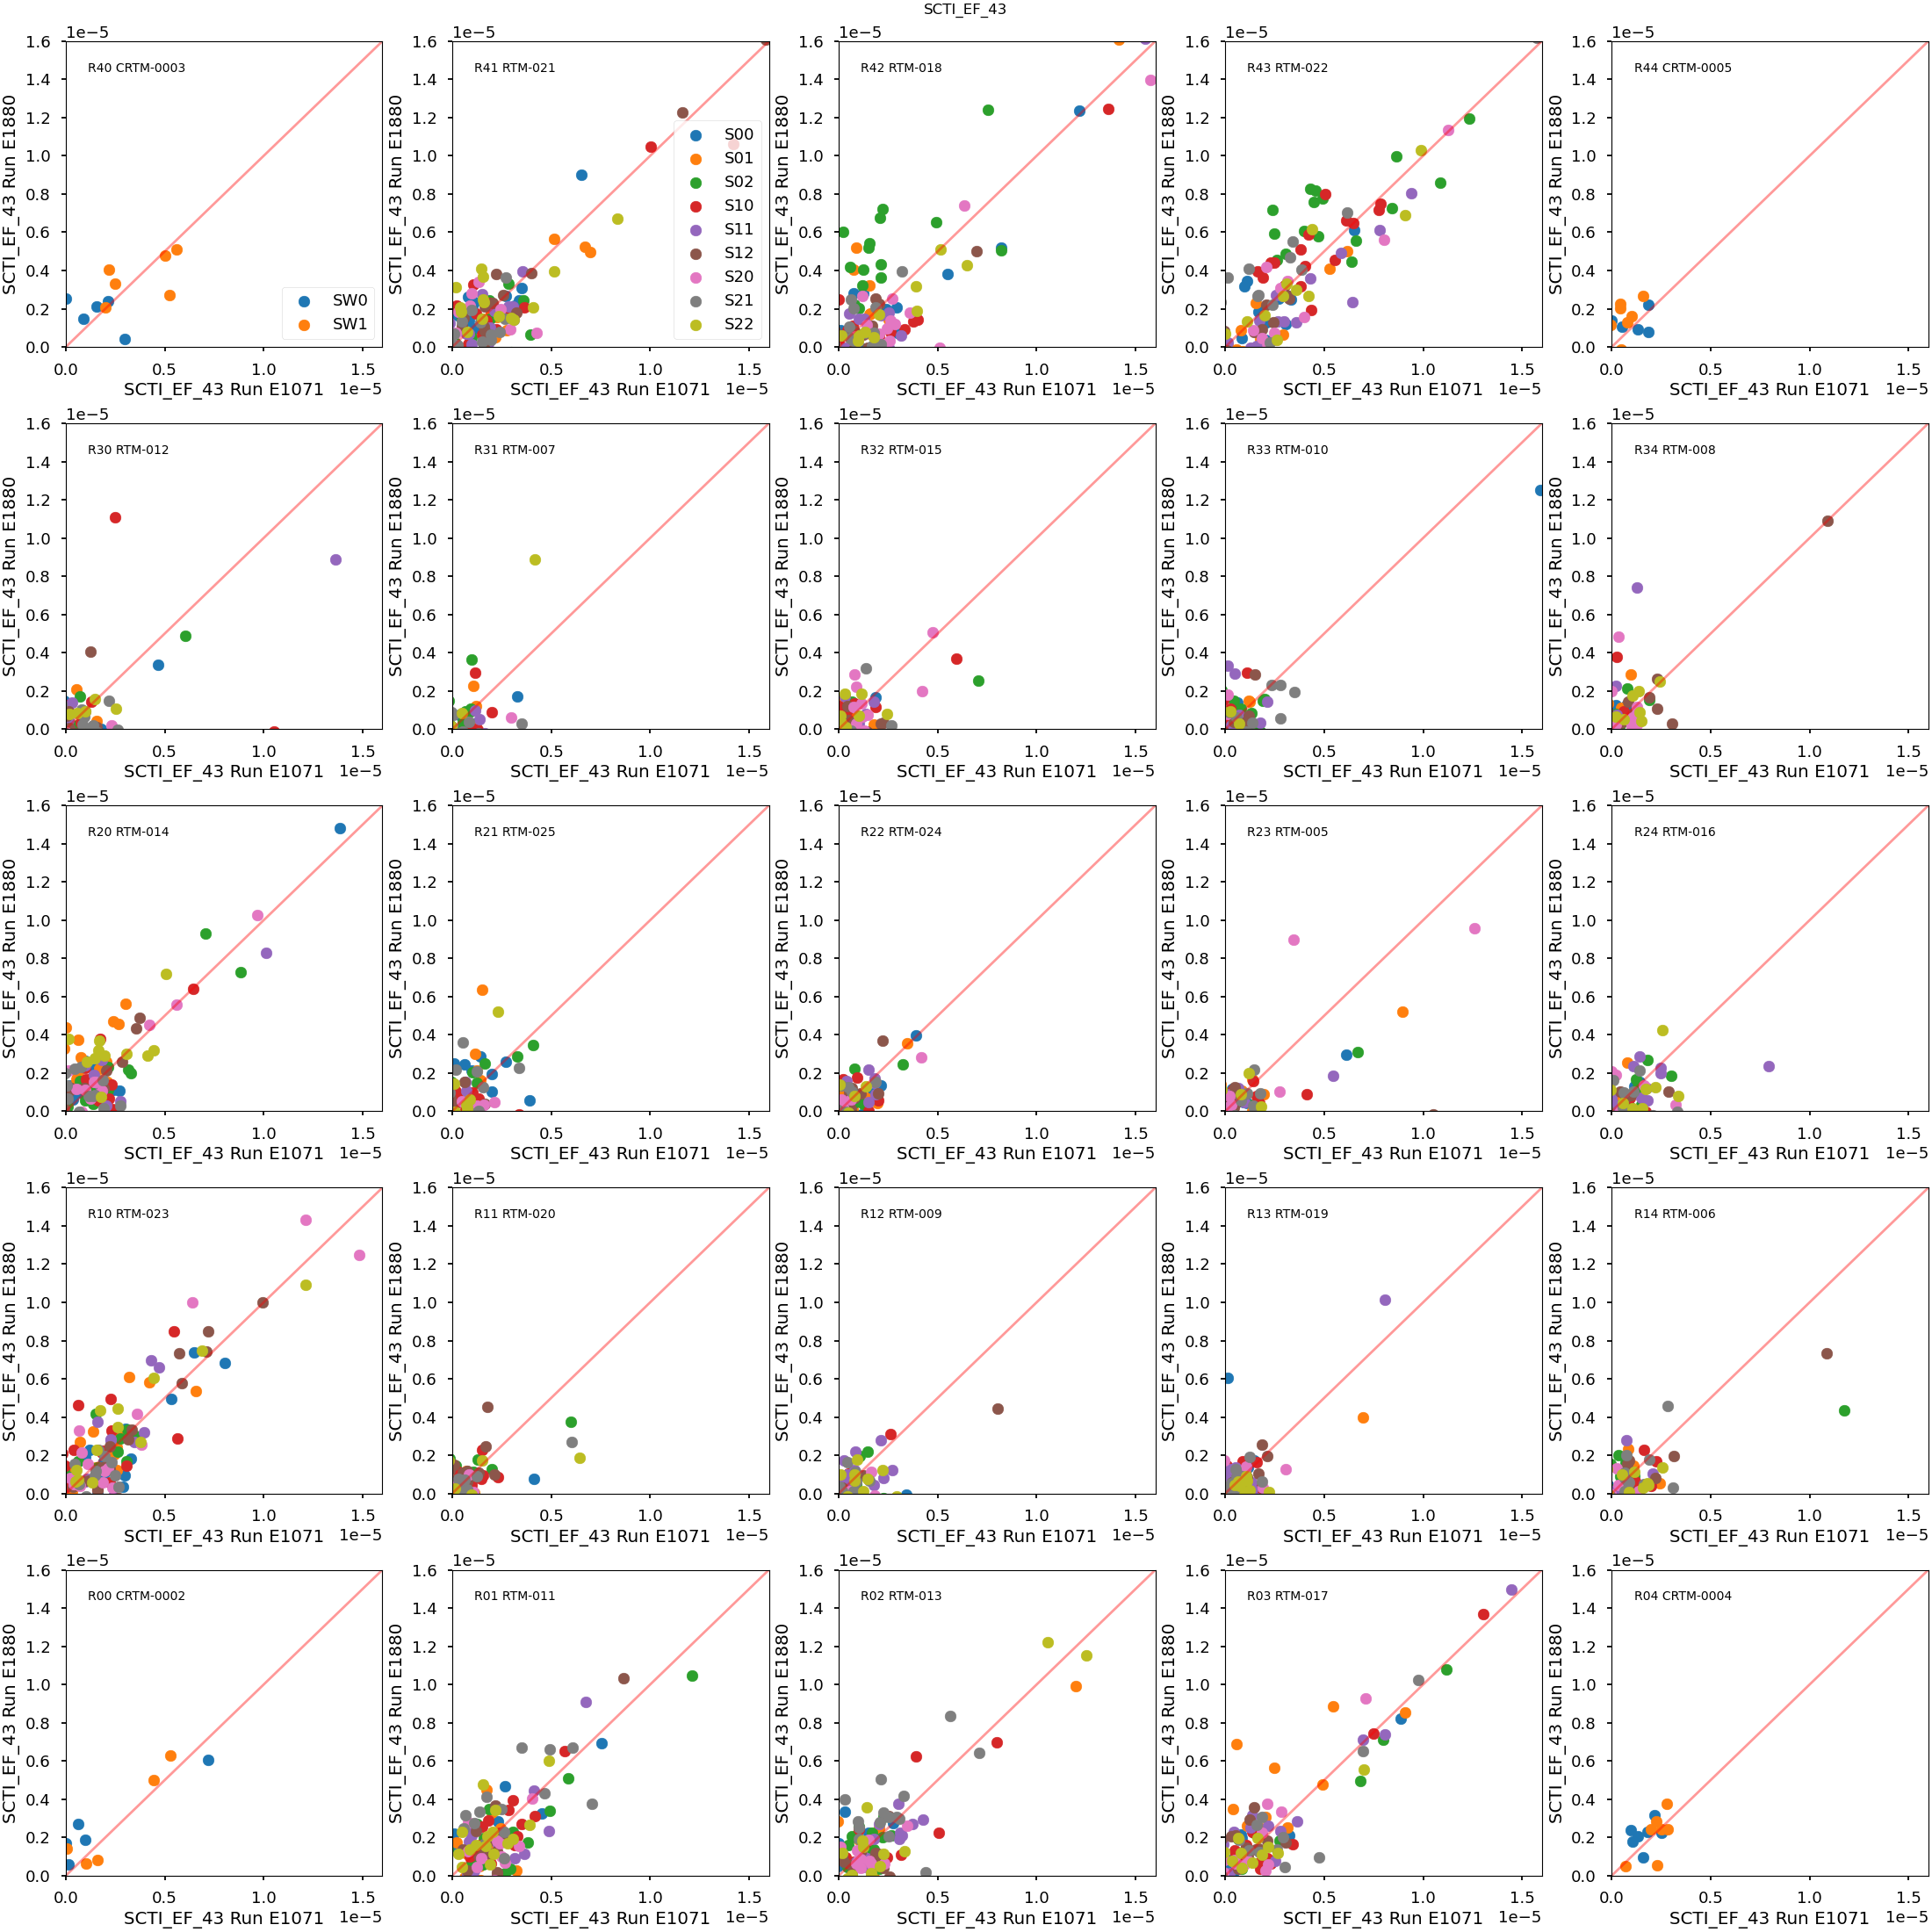
\includegraphics[width=0.7\linewidth]{figures/finalCharacterization/E1071_E1880_SCTI_EF_43_inset.png}
    \caption{Comparison of serial CTI measurements for initial and final Run 7 configurations.}
    \label{fig:finalChar-SCTI-5x5}
\end{figure}

The serial CTI for both sensor types is a noisy measurement, but serial CTI is not impacted by the changes to the LSSTCam operating configuration.

\begin{figure}[ht]
    \centering
    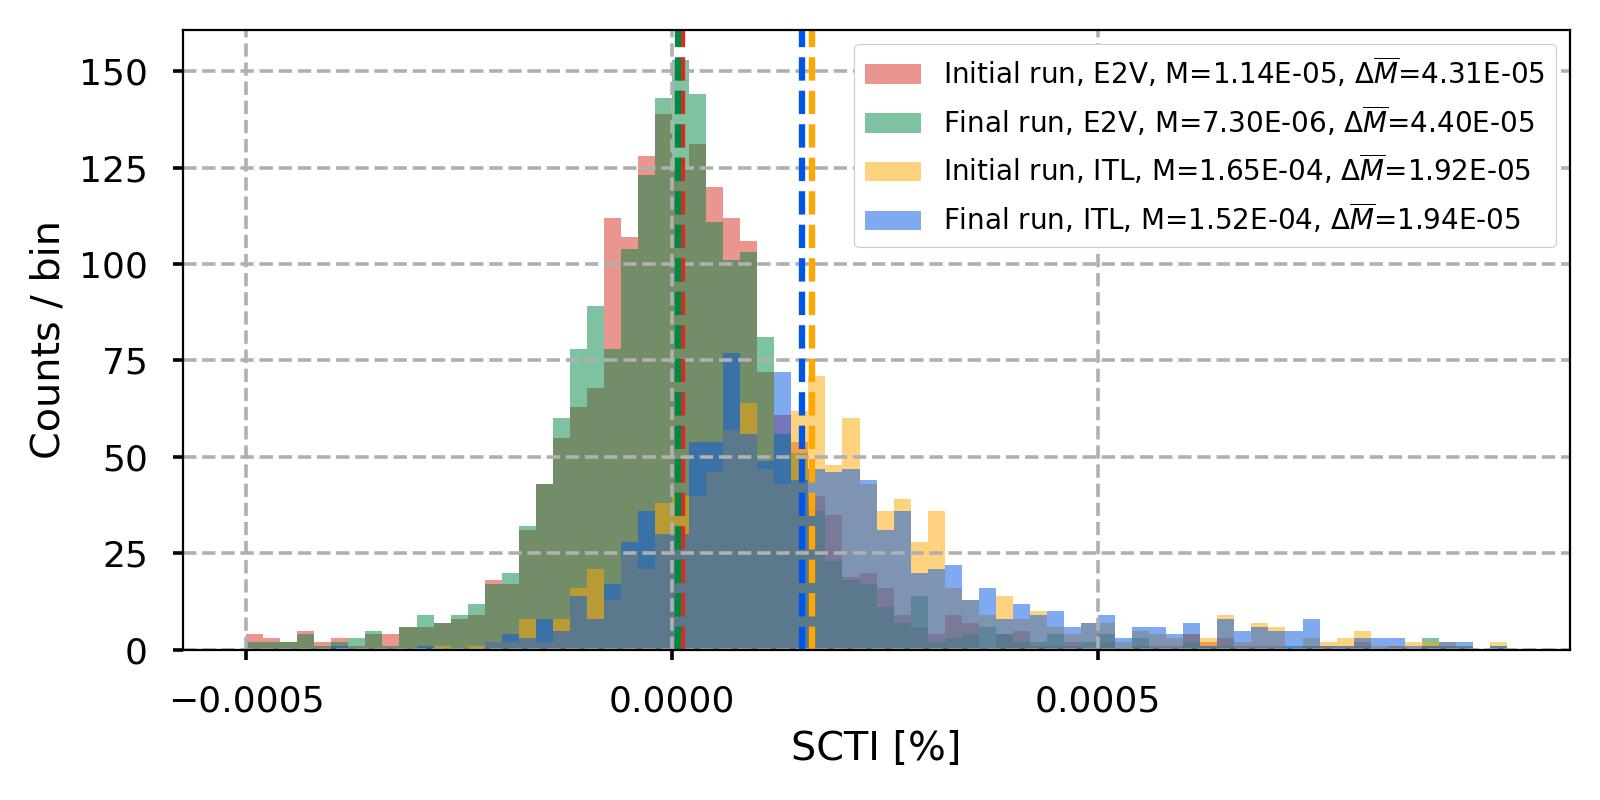
\includegraphics[width=0.7\linewidth]{figures/finalCharacterization/SCTIComp(6).jpg}
    \caption{Histogram of serial CTI measurements for initial and final Run 7 configurations, by detector type. The black lines denote median measurements for the different subgroups of measurements (e2v, ITL, initial Run 7, final Run 7).}
    \label{fig:finalChar-SCTI-hist}
\end{figure}

\clearpage


\paragraph{Parallel CTI}\label{sec:finalChar-parallel-cti}

Parallel CTI is extracted from the B protocol runs, and the values are consistent between initial and final Run 7 configurations.

\begin{figure}[ht]
    \centering
    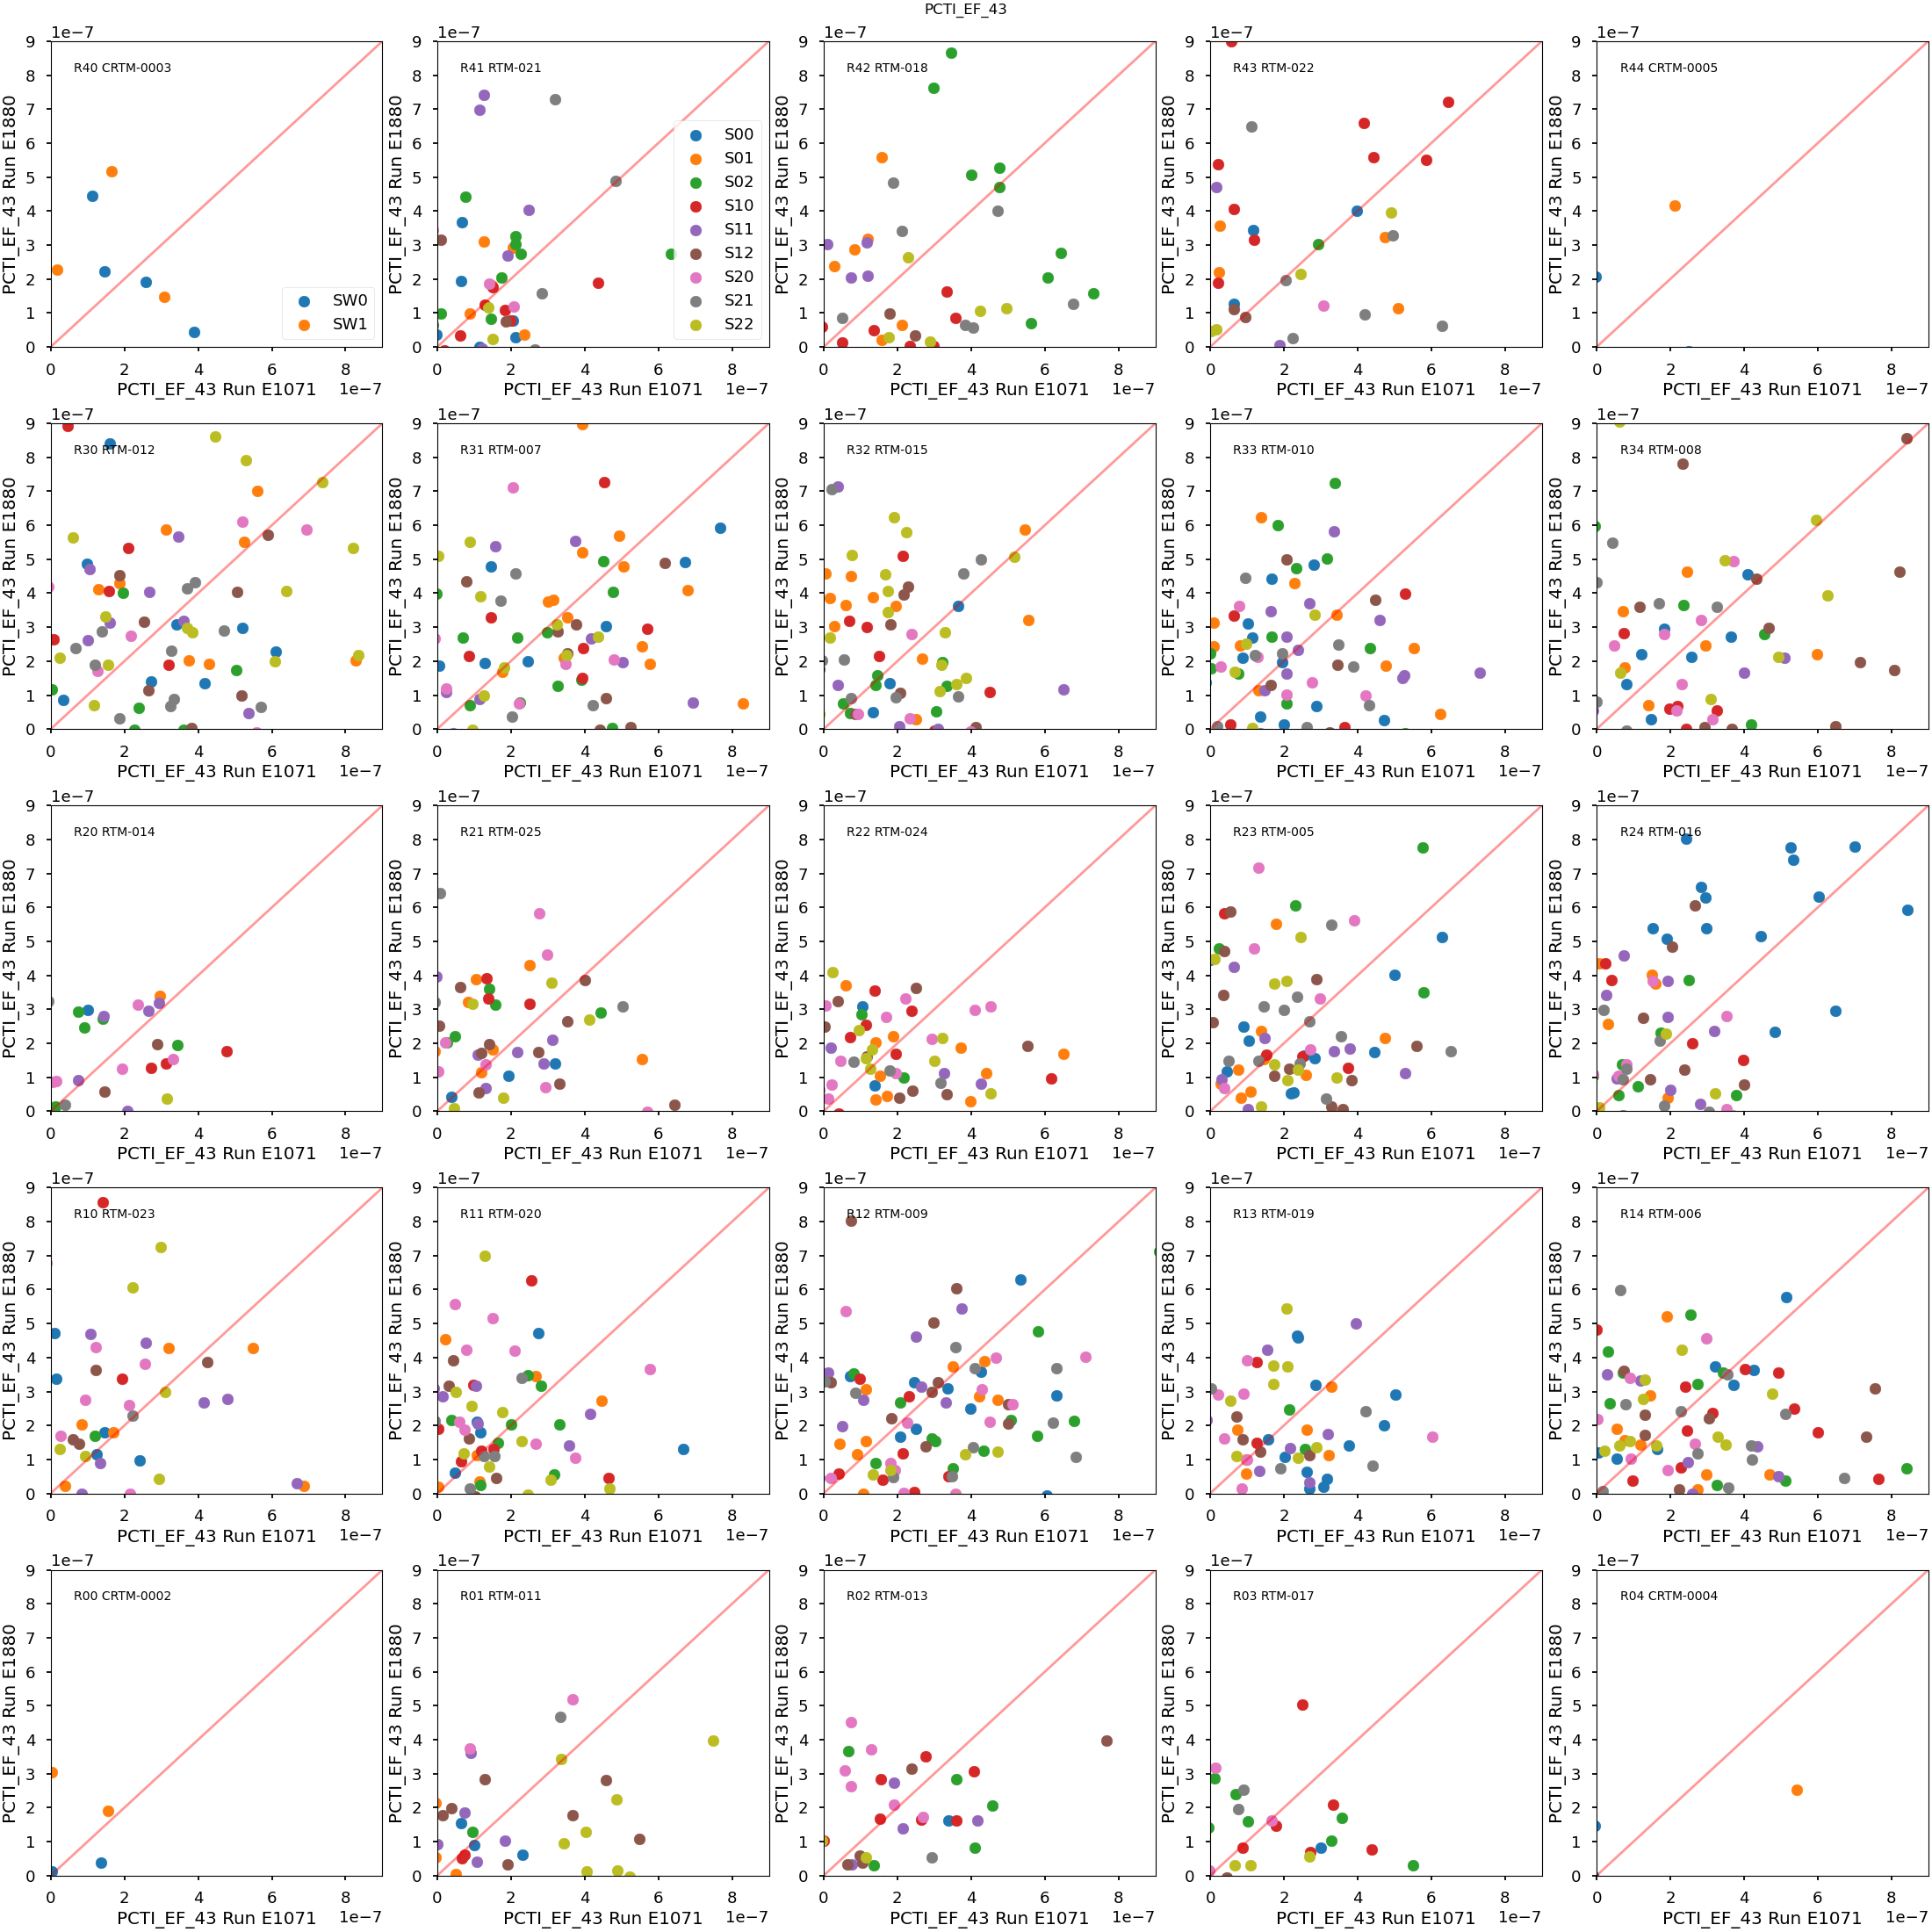
\includegraphics[width=0.7\linewidth]{figures/finalCharacterization/E1071_E1880_PCTI_EF_43_inset.png}
    \caption{Comparison of parallel CTI measurements for initial and final Run 7 configurations.}
    \label{fig:finalChar-PCTI-5x5}
\end{figure}

Similar to serial CTI, the parallel CTI for both sensor types is a noisy measurement, but is not impacted by the changes to the LSSTCam operating configuration (Fig.~\ref{fig:finalChar-PCTI-hist}).

\begin{figure}[ht]
    \centering
    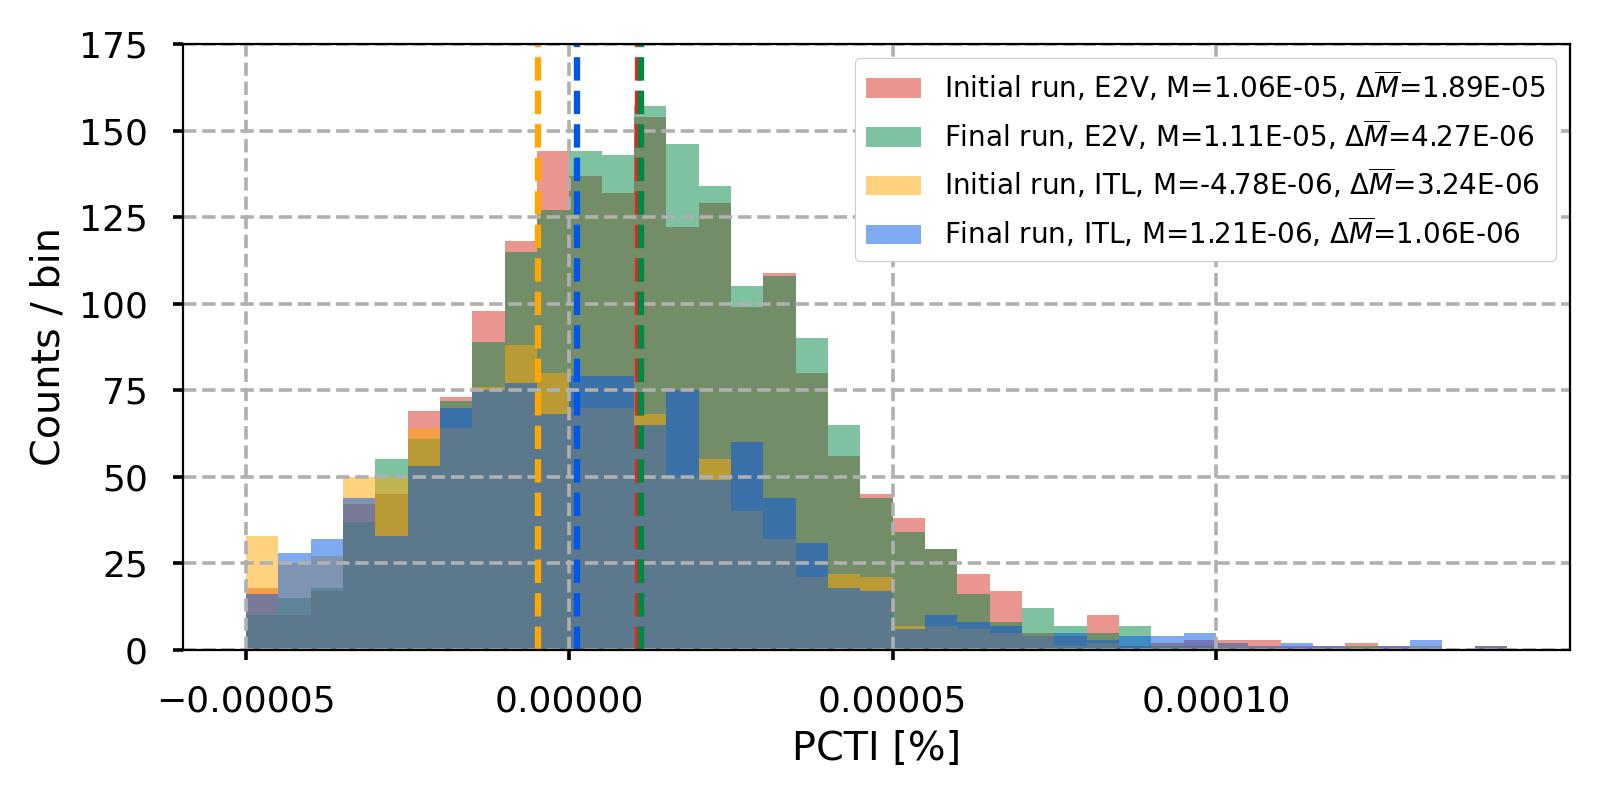
\includegraphics[width=0.7\linewidth]{figures/finalCharacterization/PCTIComp(3).jpg}
    \caption{Histogram of parallel CTI measurements for initial and final Run 7 configurations, separated by detector type. The vertical black lines denote the median values of the different histogram populations, and are displayed in the legend.}
    \label{fig:finalChar-PCTI-hist}
\end{figure}

\clearpage

\subsubsection{Dark metrics}\label{final-dark-metrics}

\paragraph{Dark current}\label{sec:finaldark-current}

Dark current measurements were extracted from the B protocol runs. Across the focal plane, dark current measurements are consistent between the initial and final Run 7 runs (Fig.~\ref{fig:finalChar-DarkCurrent-5x5}. In a subset of rafts (R13, R14, R24), a notable decrease in dark current is observed. These rafts are illuminated by the autochanger light leak, which was not mitigated until after E1880 (see Sec.~\ref{successful-autochanger-light-leaks-masking}). The physical source of the improvement in these rafts is not clear.

\begin{figure}[ht]
    \centering
    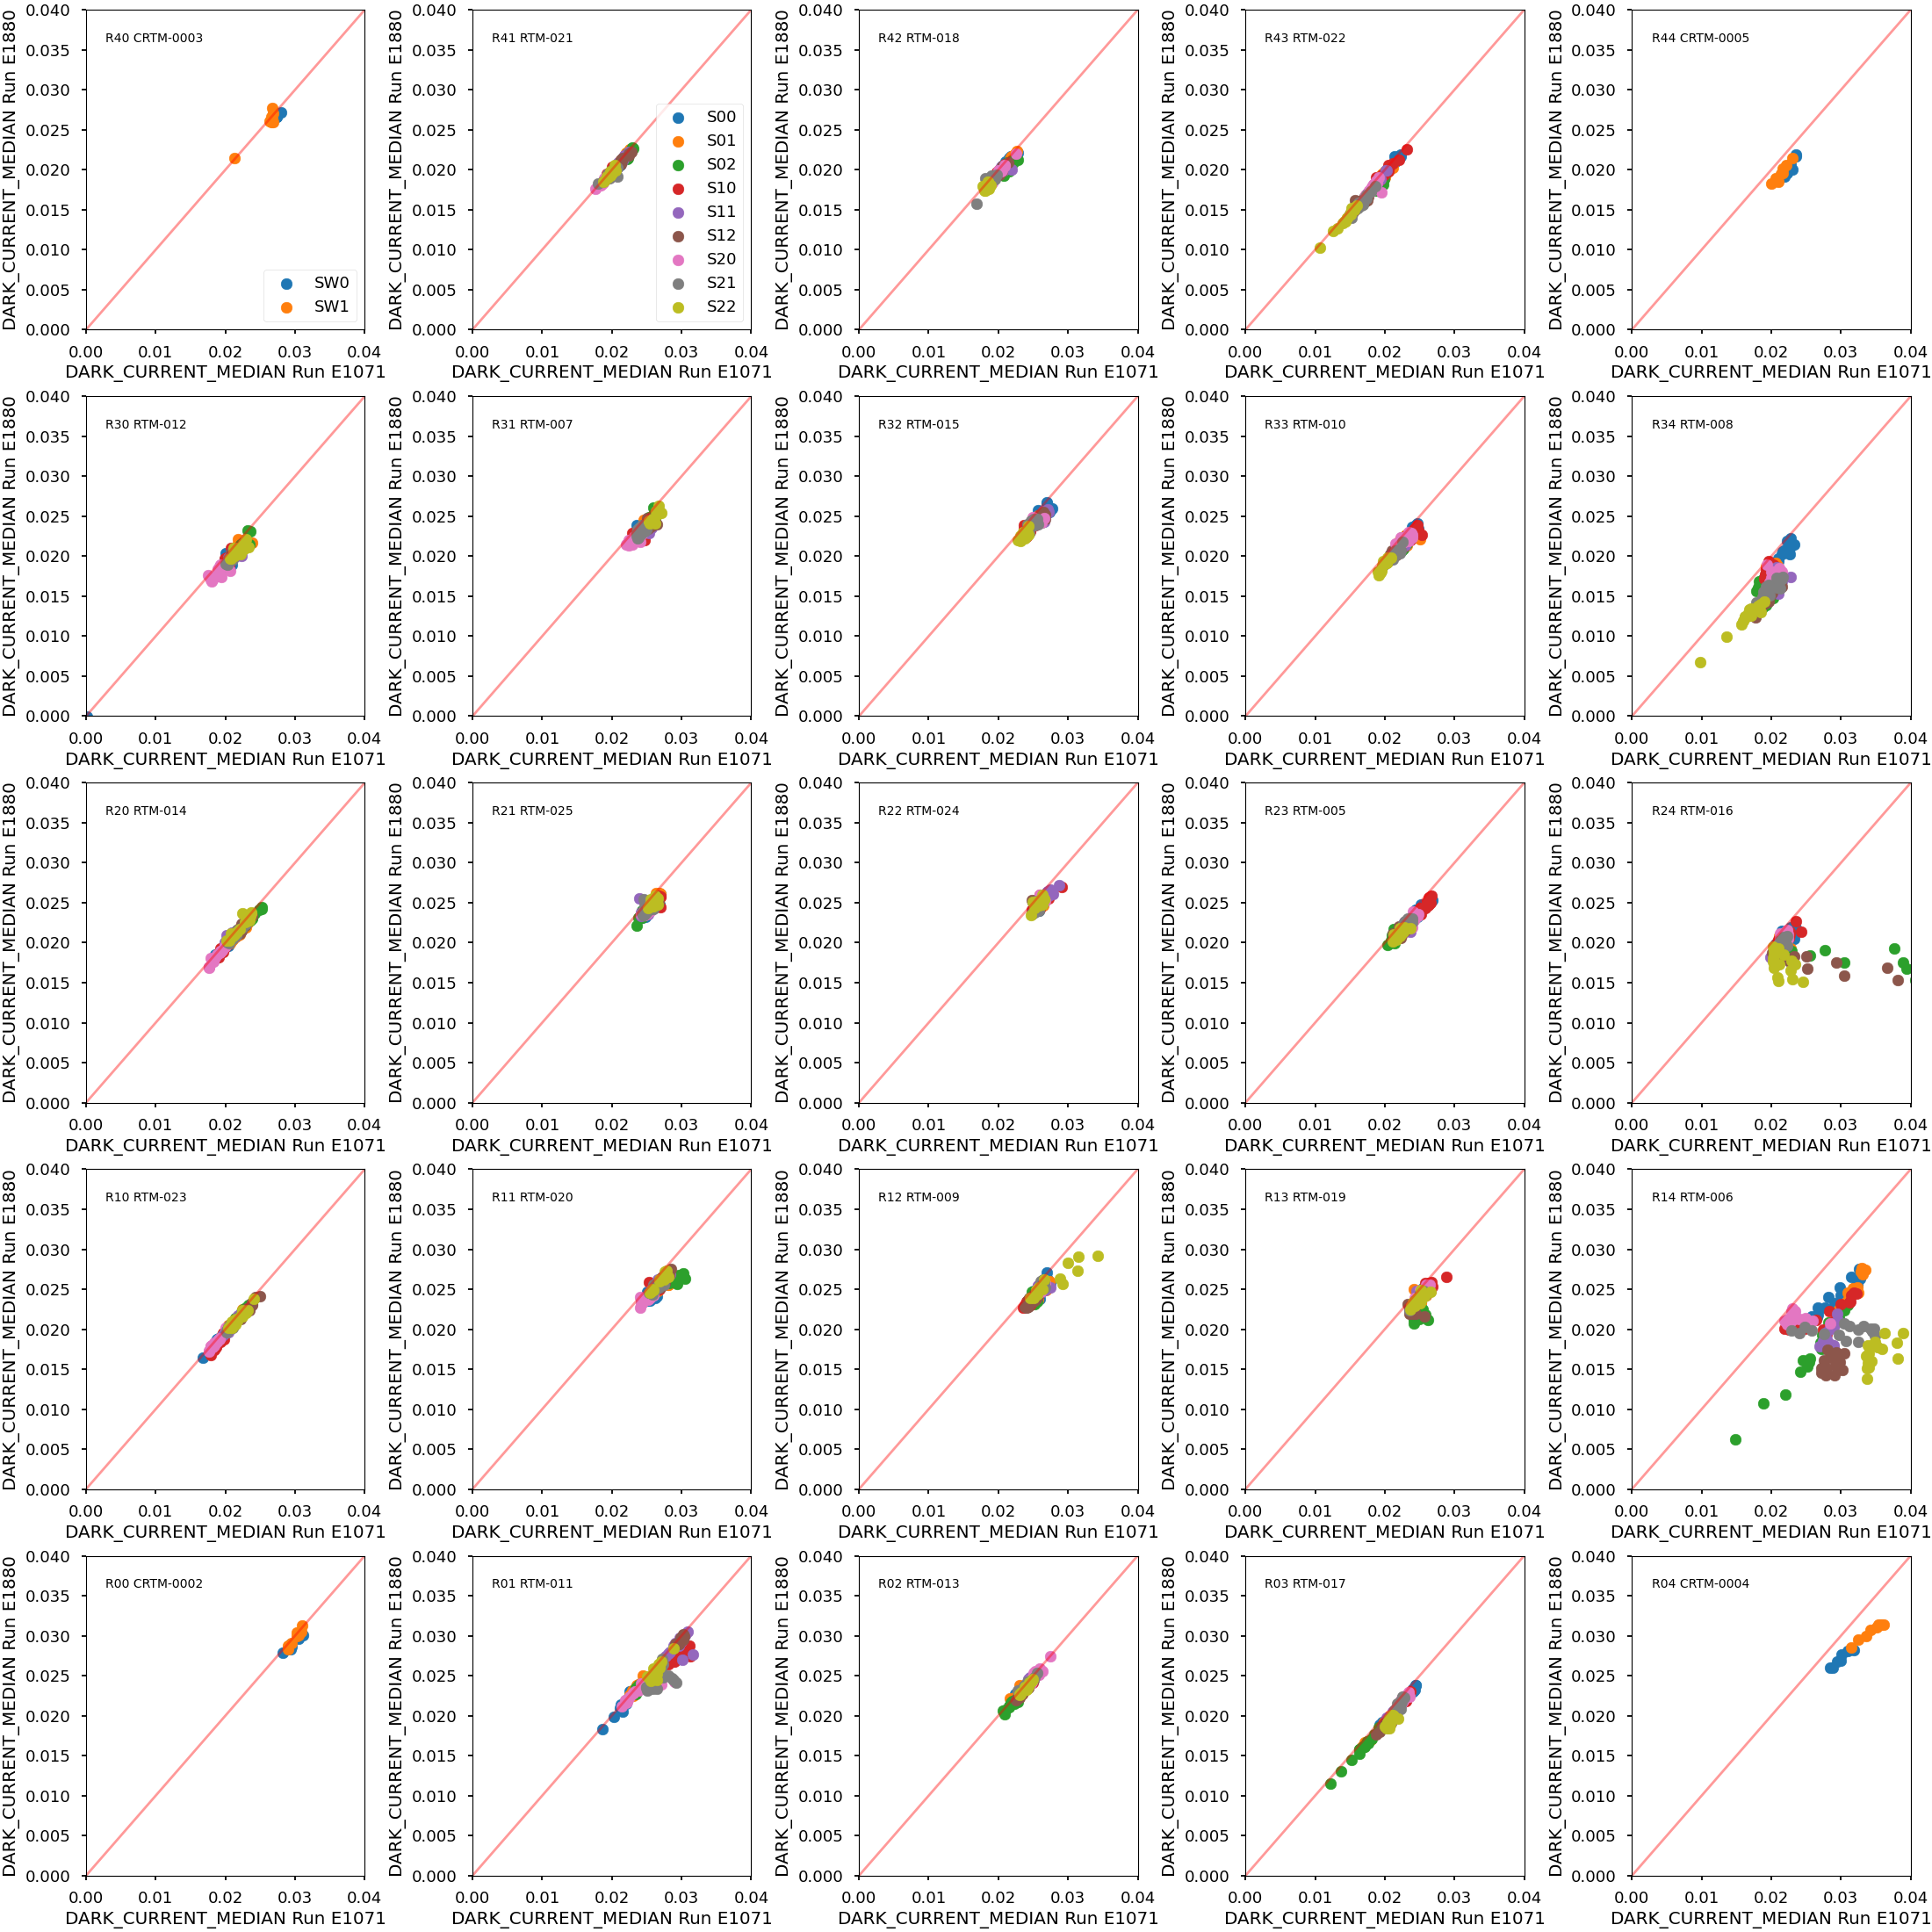
\includegraphics[width=0.7\linewidth]{figures/finalCharacterization/E1071_E1880_DARK_CURRENT_MEDIAN.png}
    \caption{Comparison of dark currents for initial and final Run 7 measurements. A marked decrease in dark current is found for the rafts that were affected by the autochanger light leak during the initial run (see Sec.~\ref{successful-autochanger-light-leaks-masking}). R14 and R24 show significant changes in dark currents. The source of the improvement is not yet clear.}
    \label{fig:finalChar-DarkCurrent-5x5}
\end{figure}

The reduction in dark current in the subset of rafts is indicative of light leak mitigation, and the final dark currents of those rafts are similar to the rest of the focal plane. One possible source of this improvement is improved shrouding in the region of these rafts.

\clearpage

\paragraph{Bright defects}\label{final-bright-defects}

Bright defects are extracted using the B protocol runs, and the agreement between runs is extremely close (Fig.~\ref{fig:finalChar-BrightPixels-5x5}). No significant bright defects developed as a result of the voltage, sequencer, or idle flush condition changes.

\begin{figure}[ht]
    \centering
    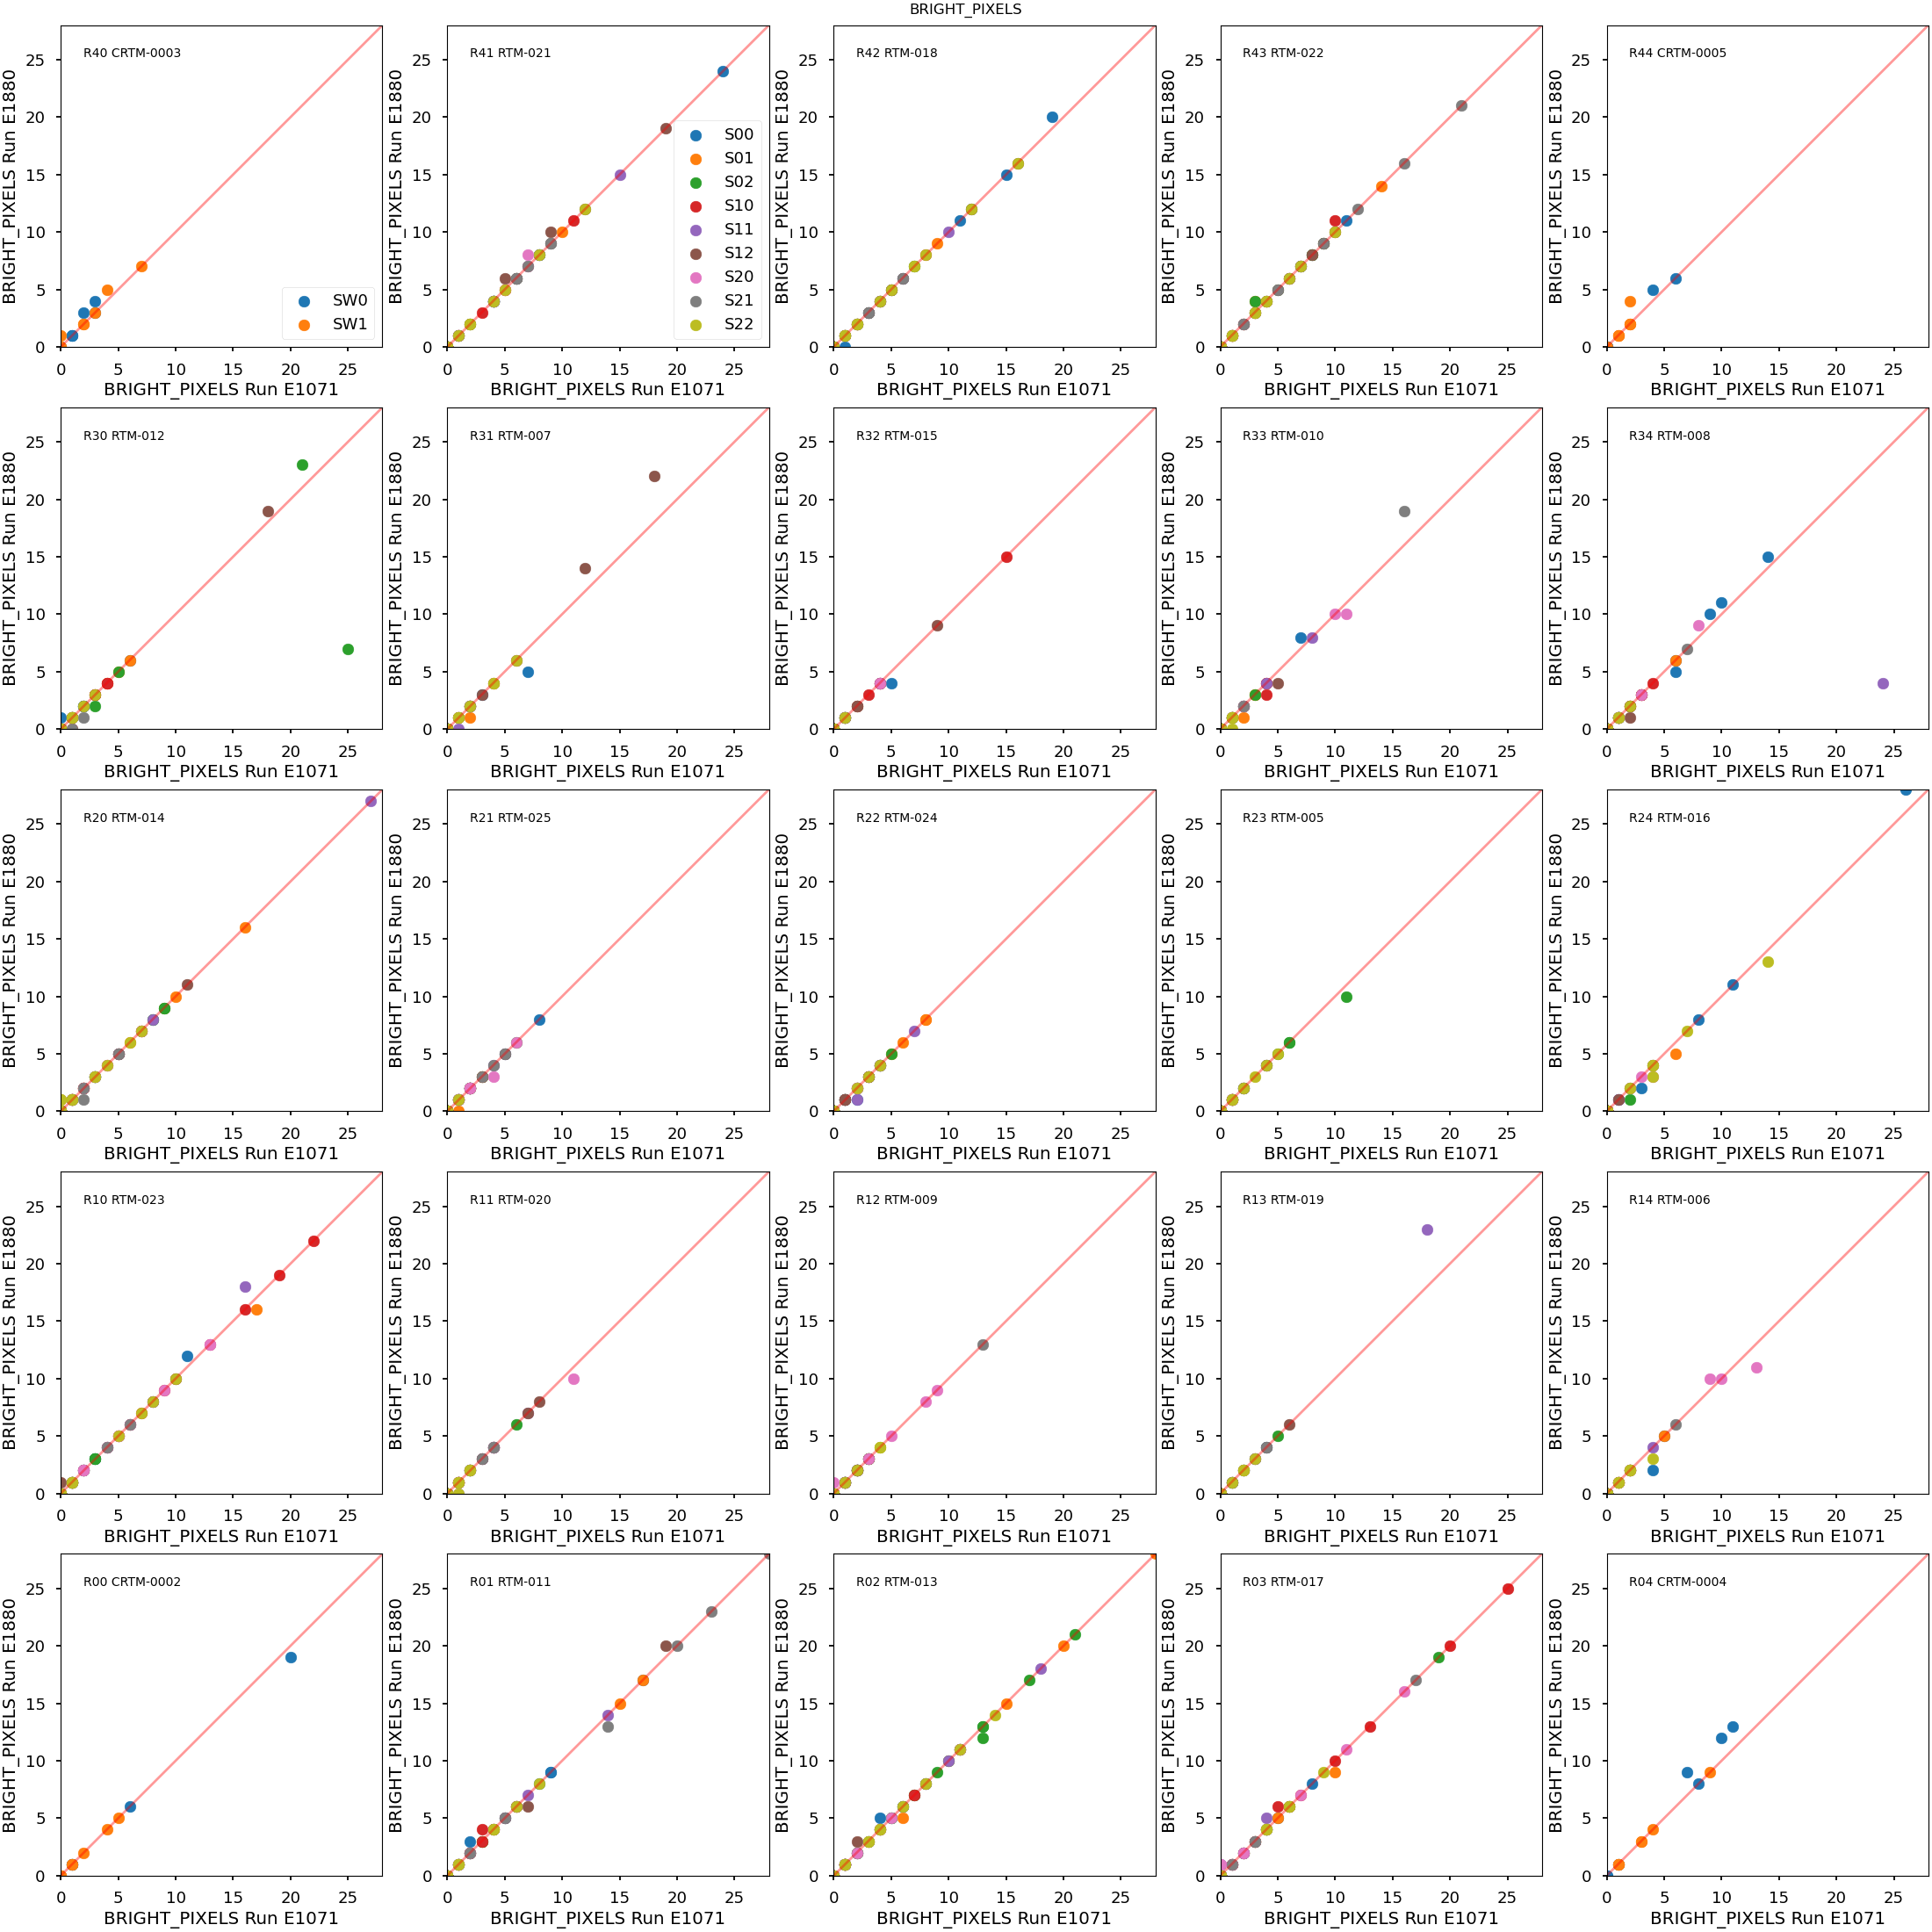
\includegraphics[width=0.7\linewidth]{figures/finalCharacterization/E1071_E1880_BRIGHT_PIXELS.png}
    \caption{Comparison of bright pixels for initial and final Run 7 measurements. Each point is organized into subplots by raft. Each sensor is plotted in different colors. Measurements are made for each segment, resulting in multiple points with the same color on the same subplot.}
    \label{fig:finalChar-BrightPixels-5x5}
\end{figure}

Two segments that improved significantly were R30\_S02\_C17 and R34\_S11\_C12 shown in Figure \ref{fig:finalChar-BrightPixels-5x5}. Both of these segments exhibited columns with higher response. In the final operating configuration, the spatial area of this response decreased, resulting in the improvement in the bright defect measurement.

For additional discussion about defect stability, see Section~\ref{defect-stability}.

\clearpage
\subsubsection{Flat pair metrics}

\begin{figure}[ht]
    \centering
    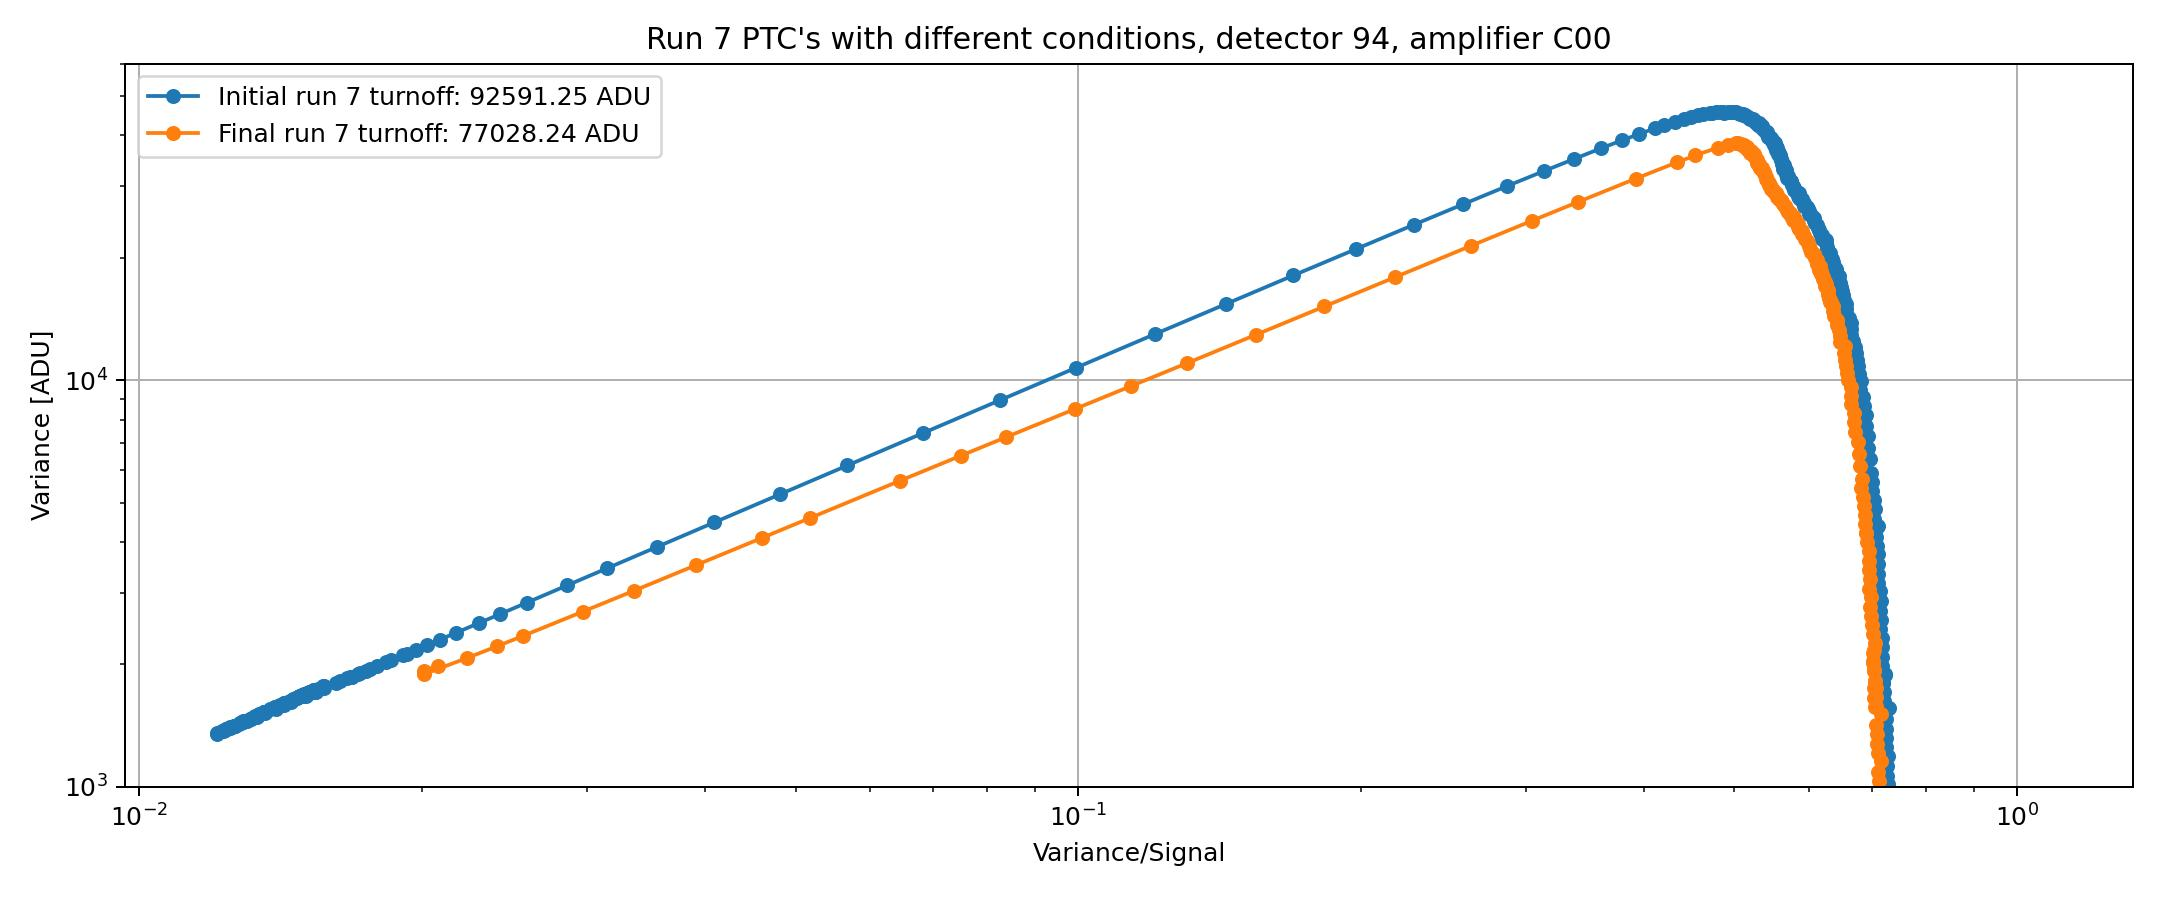
\includegraphics[width=0.7\linewidth]{figures/finalCharacterization/run7PTCsToDate(3).jpg}
    \caption{Comparison of PTCs from initial and final Run 7 conditions, for R22\_S11\_C00.}
    \label{fig:finalChar-PTCComparison}
\end{figure}
\clearpage

\paragraph{Linearity and PTC turnoff}\label{final-linearity-and-ptc-turnoff}

Both linearity and PTC turnoff were evaluated from the PTC runs (Fig.~\ref{fig:finalChar-Linearity-5x5} and Fig.~\ref{fig:finalChar-PTCTurnoff-5x5}). Due to a decrease in parallel swing voltage for e2v sensors between initial and final Run 7 runs, we anticipate a lower full-well capacity by either linearity or PTC turnoff measure (see \cite{2001sccd.book.....J}). As described in Section~\ref{persistence-optimization-1}, we observe a decrease in full-well capacity for e2v sensors. ITL sensors exhibit stable full-well capacities, despite the changes to the v30 sequencer and disablement of the idle flush (see Secs.~\ref{section:disablingIDLEFLUSH} and \ref{sequencer-optimization}).

\begin{figure}[ht]
    \centering
    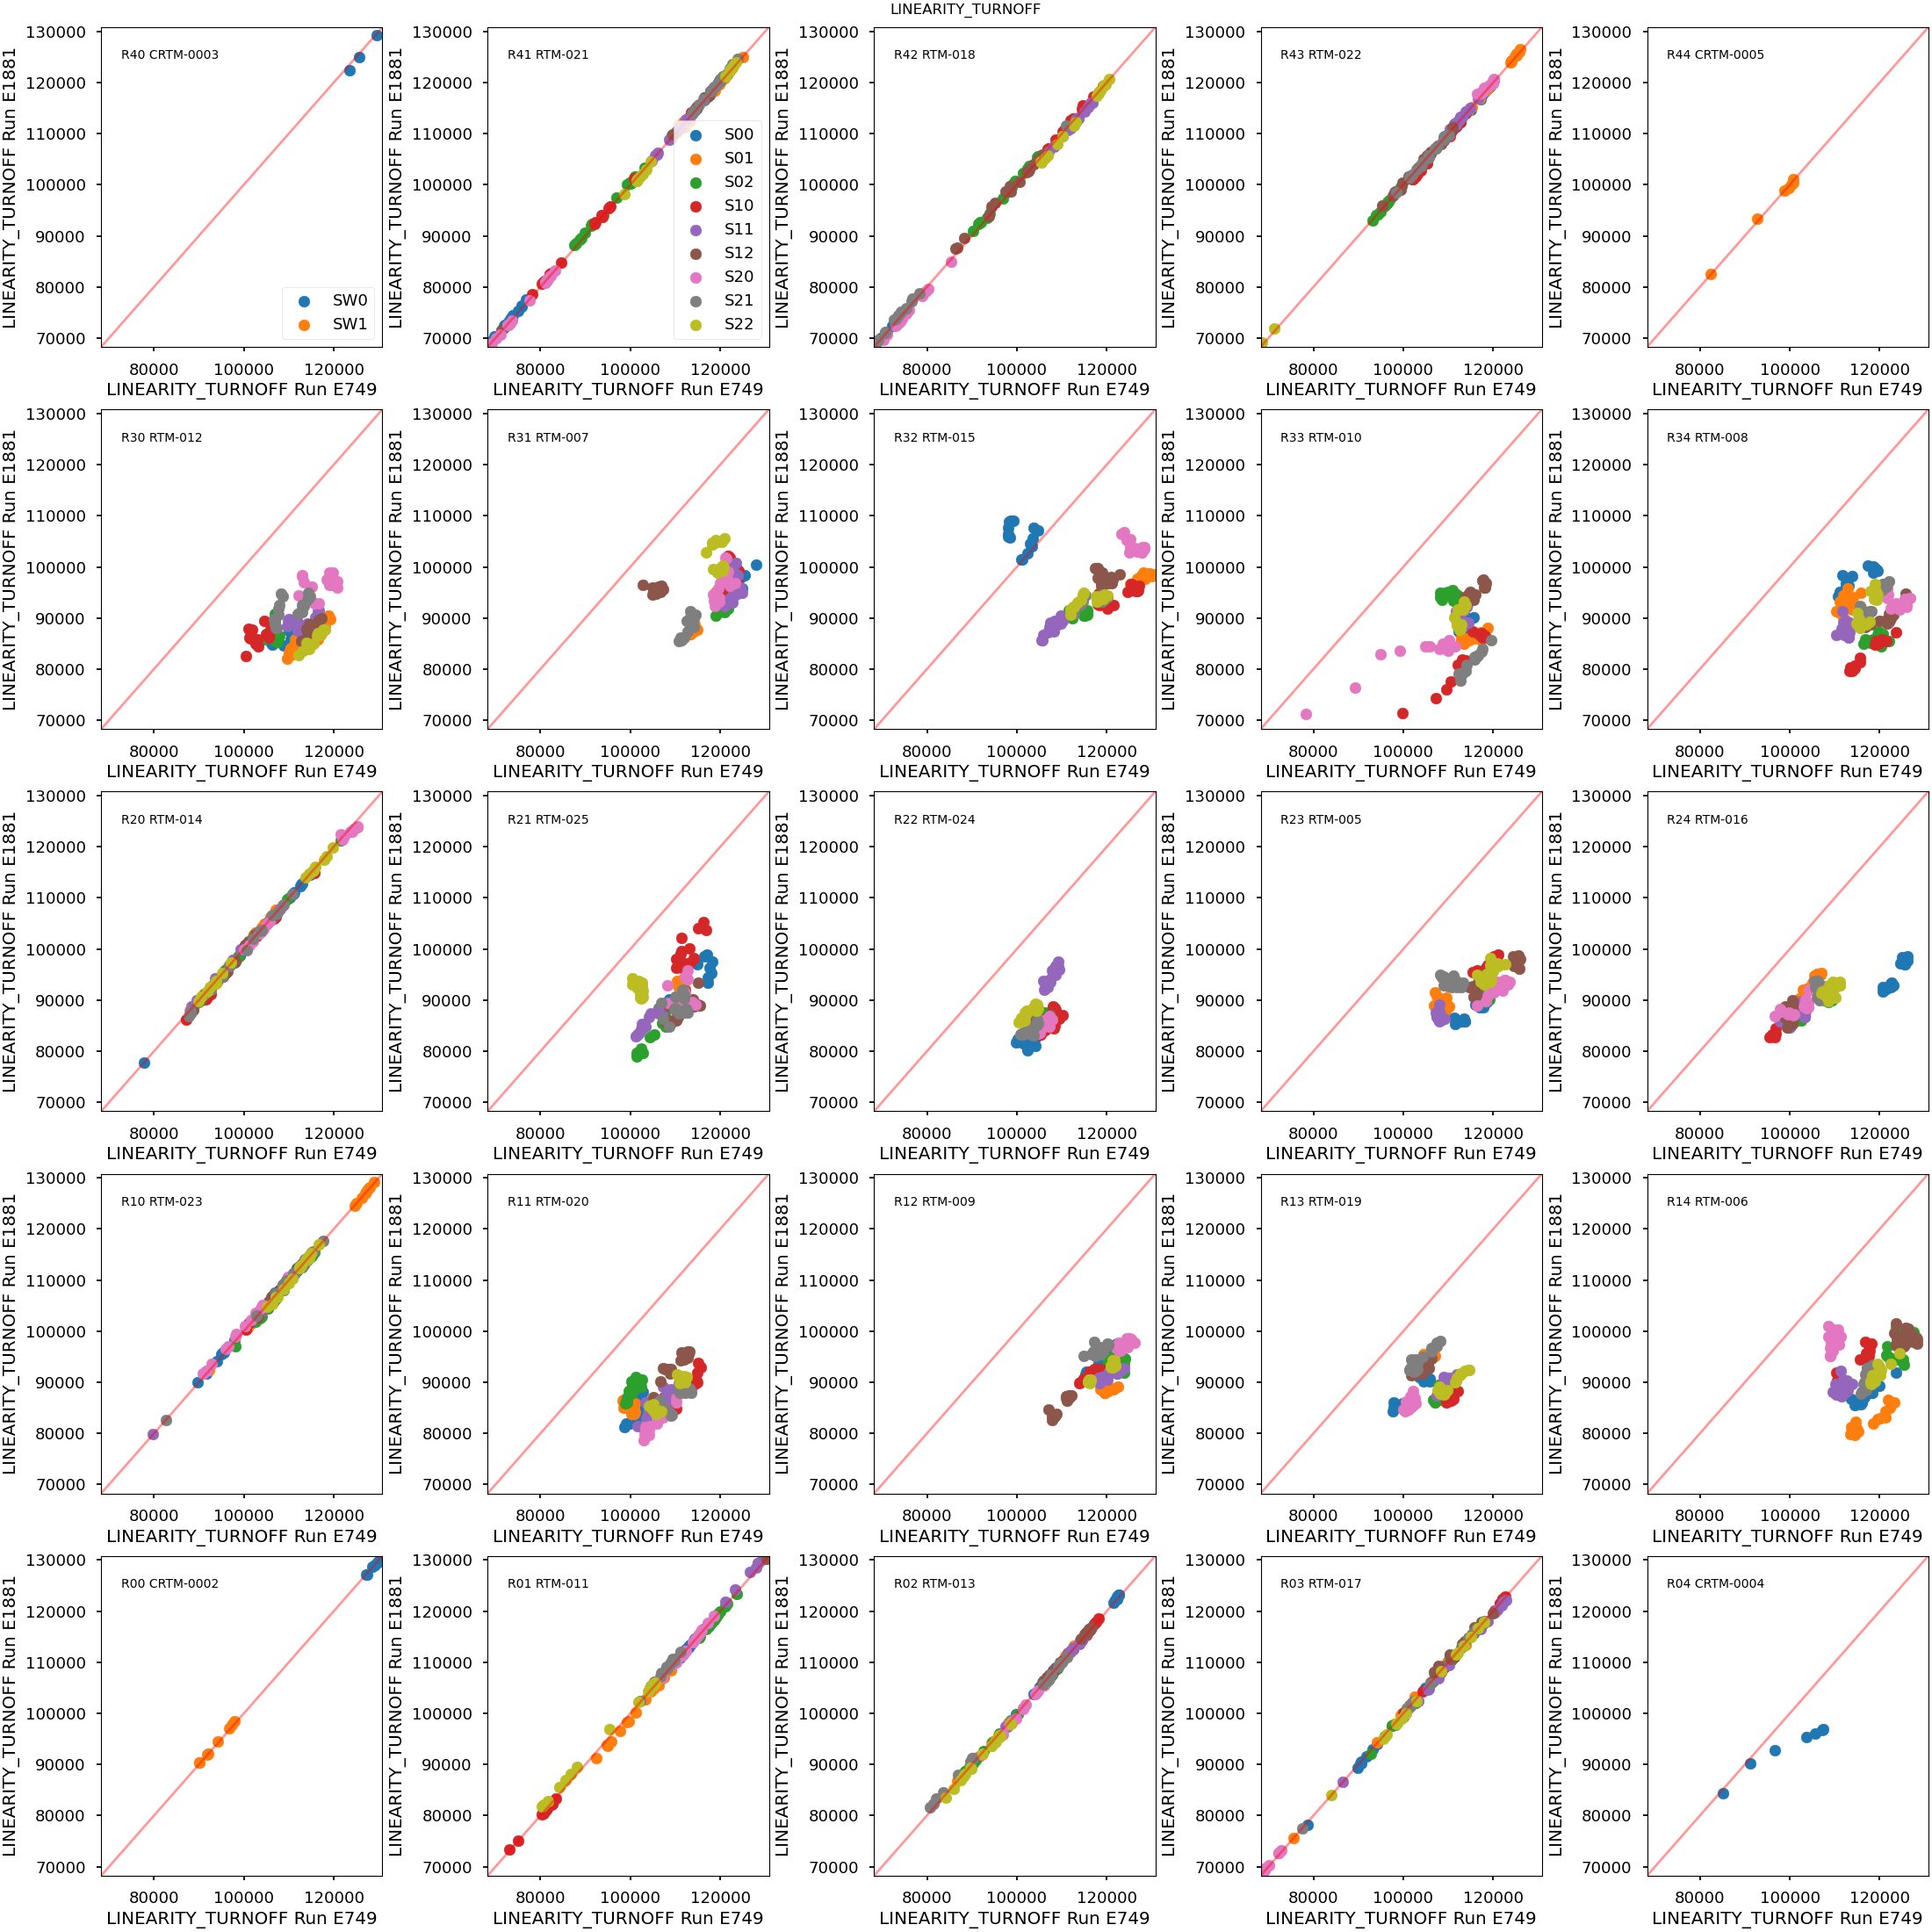
\includegraphics[width=0.7\linewidth]{figures/finalCharacterization/E749_E1881_LINEARITY_TURNOFF.png}
    \caption{Comparison of linearity turnoffs between the initial and final Run 7 measurements. The e2v sensors show a notable decrease in linearity turnoff, while ITL sensors stay the same. The values reported here are in ADU, i.e., not gain corrected.}
    \label{fig:finalChar-Linearity-5x5}
\end{figure}

For e2v sensors we find the reduction in full-well to be significant, \textasciitilde20--25\% depending on the full-well metric used (see Fig.~\ref{fig:finalChar-fullWell}).

\begin{figure}[ht]
    \centering
    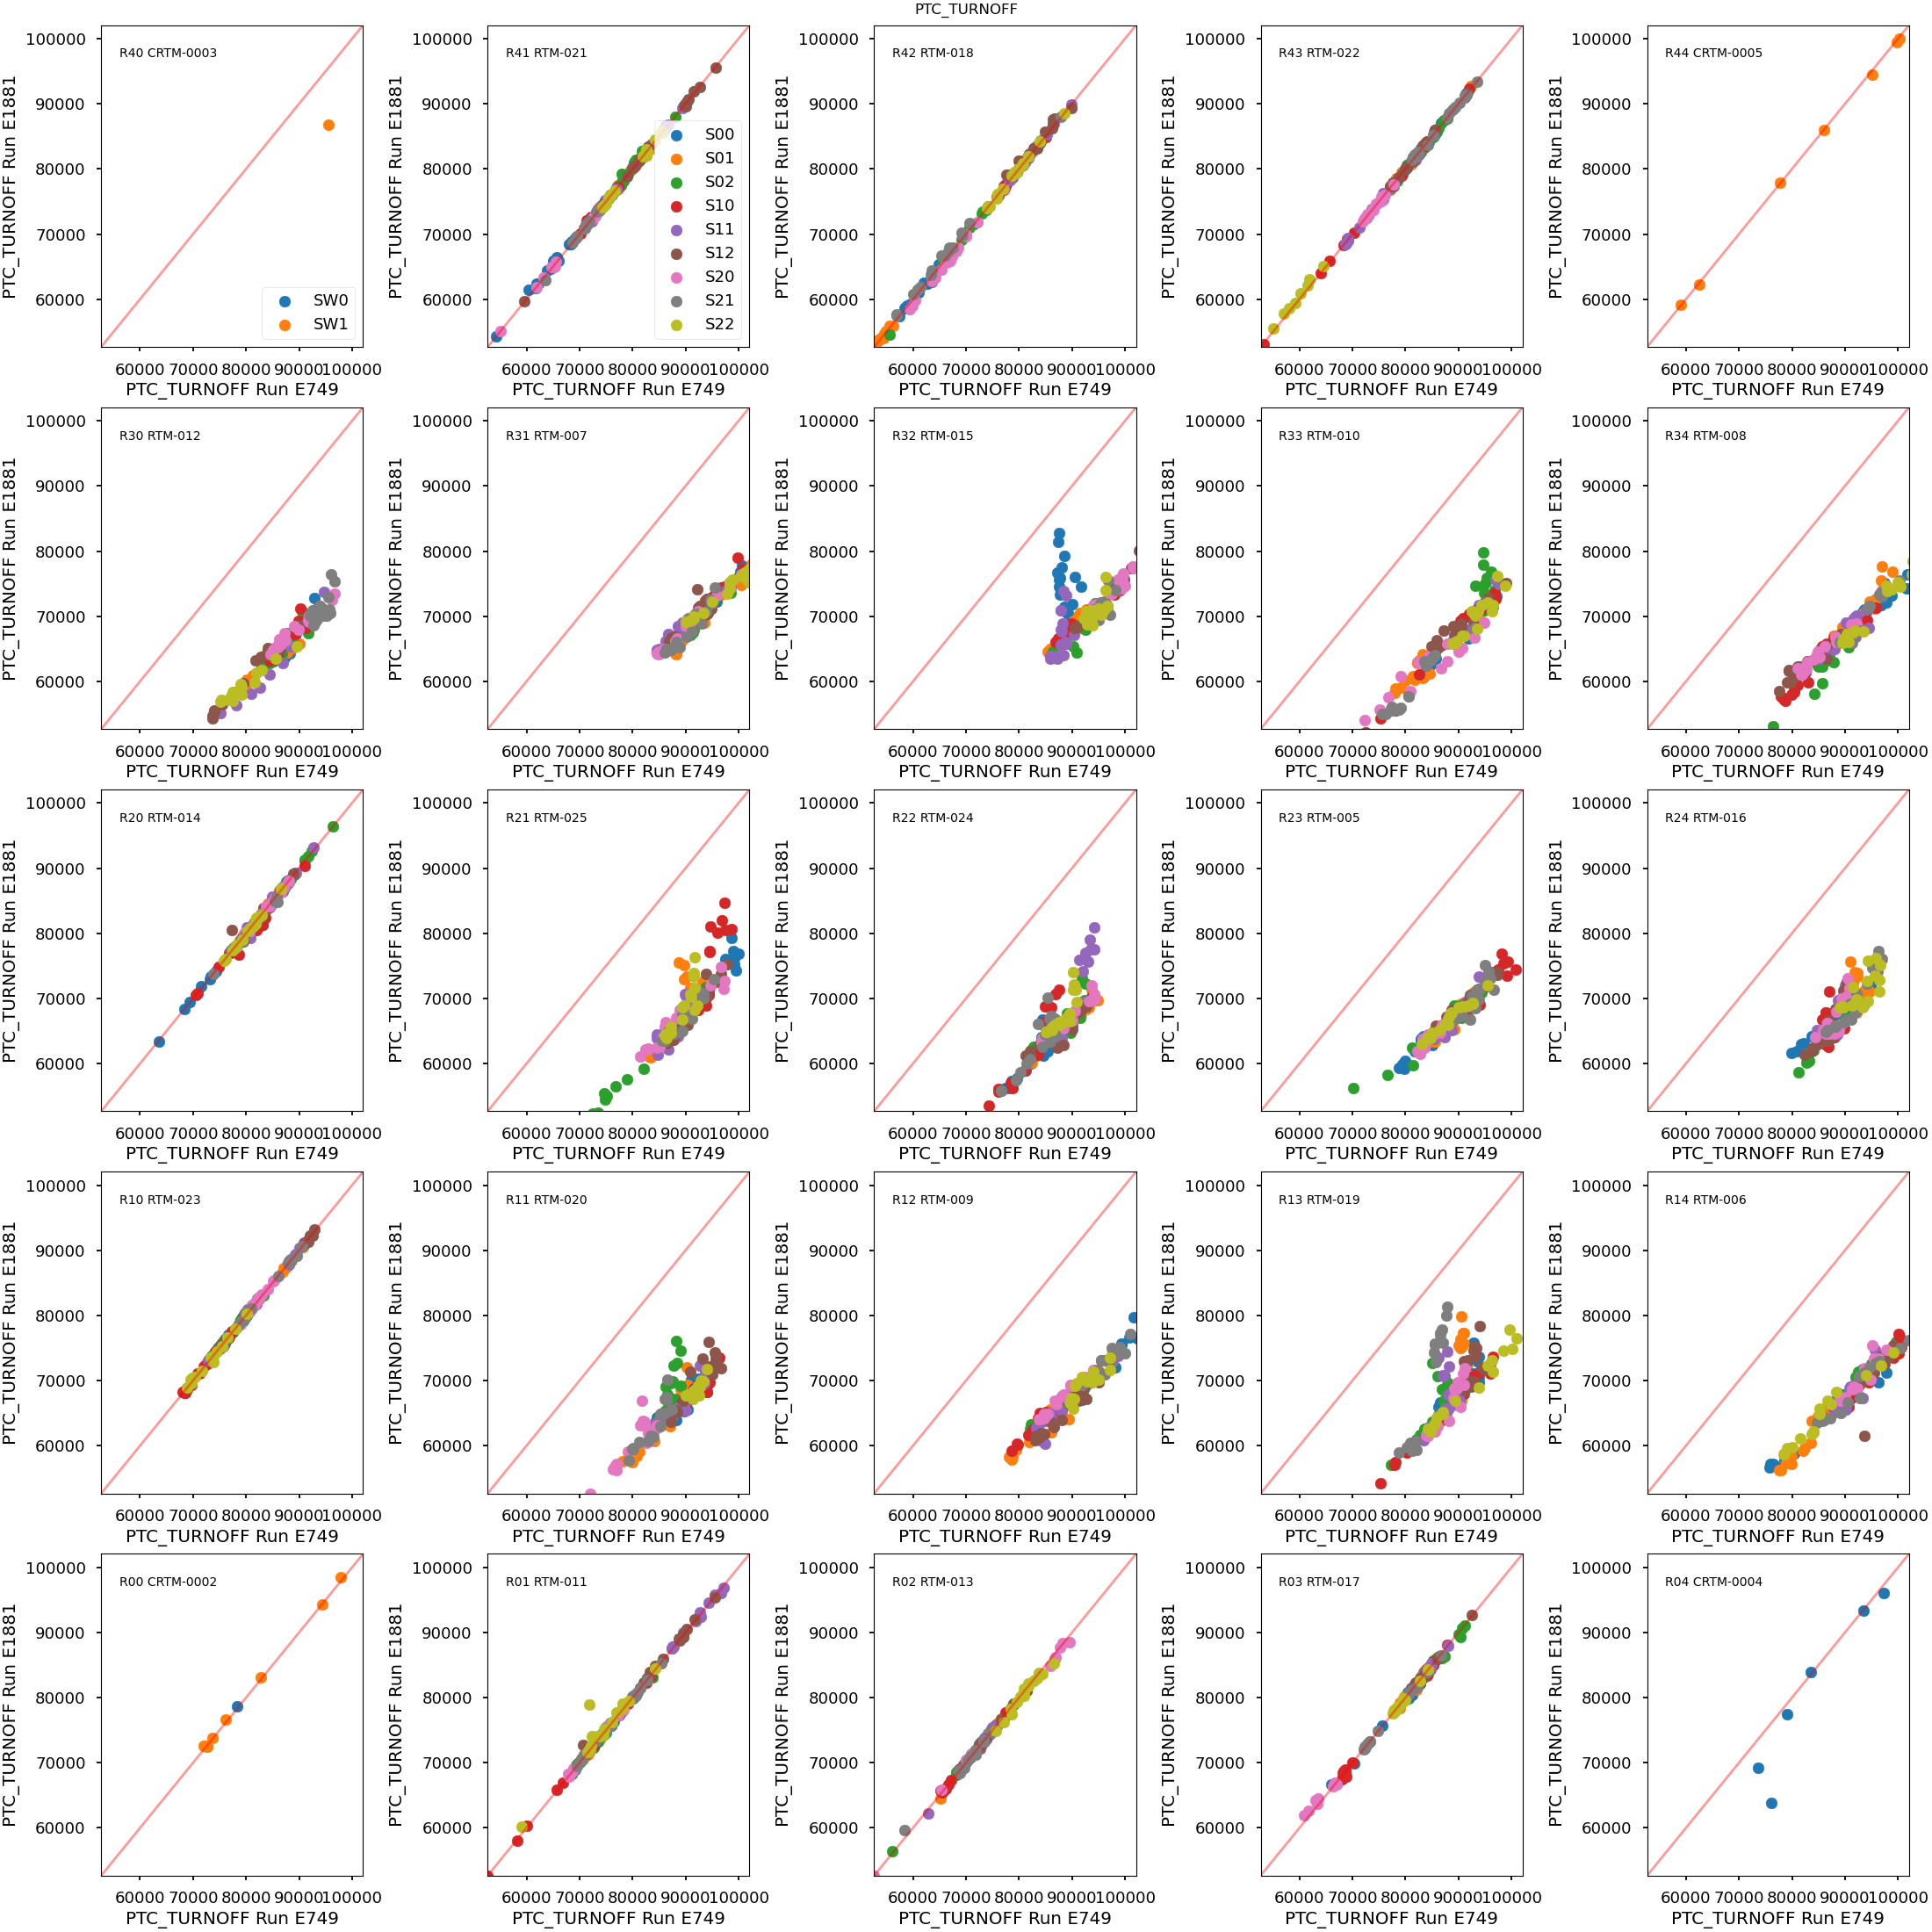
\includegraphics[width=0.7\linewidth]{figures/finalCharacterization/E749_E1881_PTC_TURNOFF.png}
    \caption{Comparison of PTC turnoff measurements from the initial and final Run 7 measurements. The e2v sensors show a notable decrease in PTC turnoff, while ITL sensors stay the same. The values reported here are in ADU, i.e., not gain corrected.}
    \label{fig:finalChar-PTCTurnoff-5x5}
\end{figure}


Since early in the planning for LSST, a 90,000 e- full-well capacity was established as a requirement for an 8 magnitude dynamic range across all bands \citep{AndyFullWell}. If linearity turnoff is the metric used to quantify full-well, all e2v amplifiers pass this system requirement. If PTC turnoff is the metric used to quantify full-well, 6.4\% of e2v amplifiers do not pass this system requirement (120/1872 total amplifiers). Photometry is possible up to the linearity turnoff without a nonlinearity correction, whereas shape measurements can be made accurately up to the PTC turnoff. Shapes are not measured at high flux, near turnoff. For these reasons, we consider this requirement passed.

In PTC turnoff (see Fig.~\ref{fig:finalChar-PTCTurnoff-5x5}), several sensors (R13\_S21 and R32\_S00) show a feature indicative of a range of values for the final Run 7 data, but a closer distribution of values in the initial Run 7 data. The reason for this difference in distributions is not clear. Both of these sensors pass the PTC turnoff requirement.

\begin{figure}[ht]
    \centering
    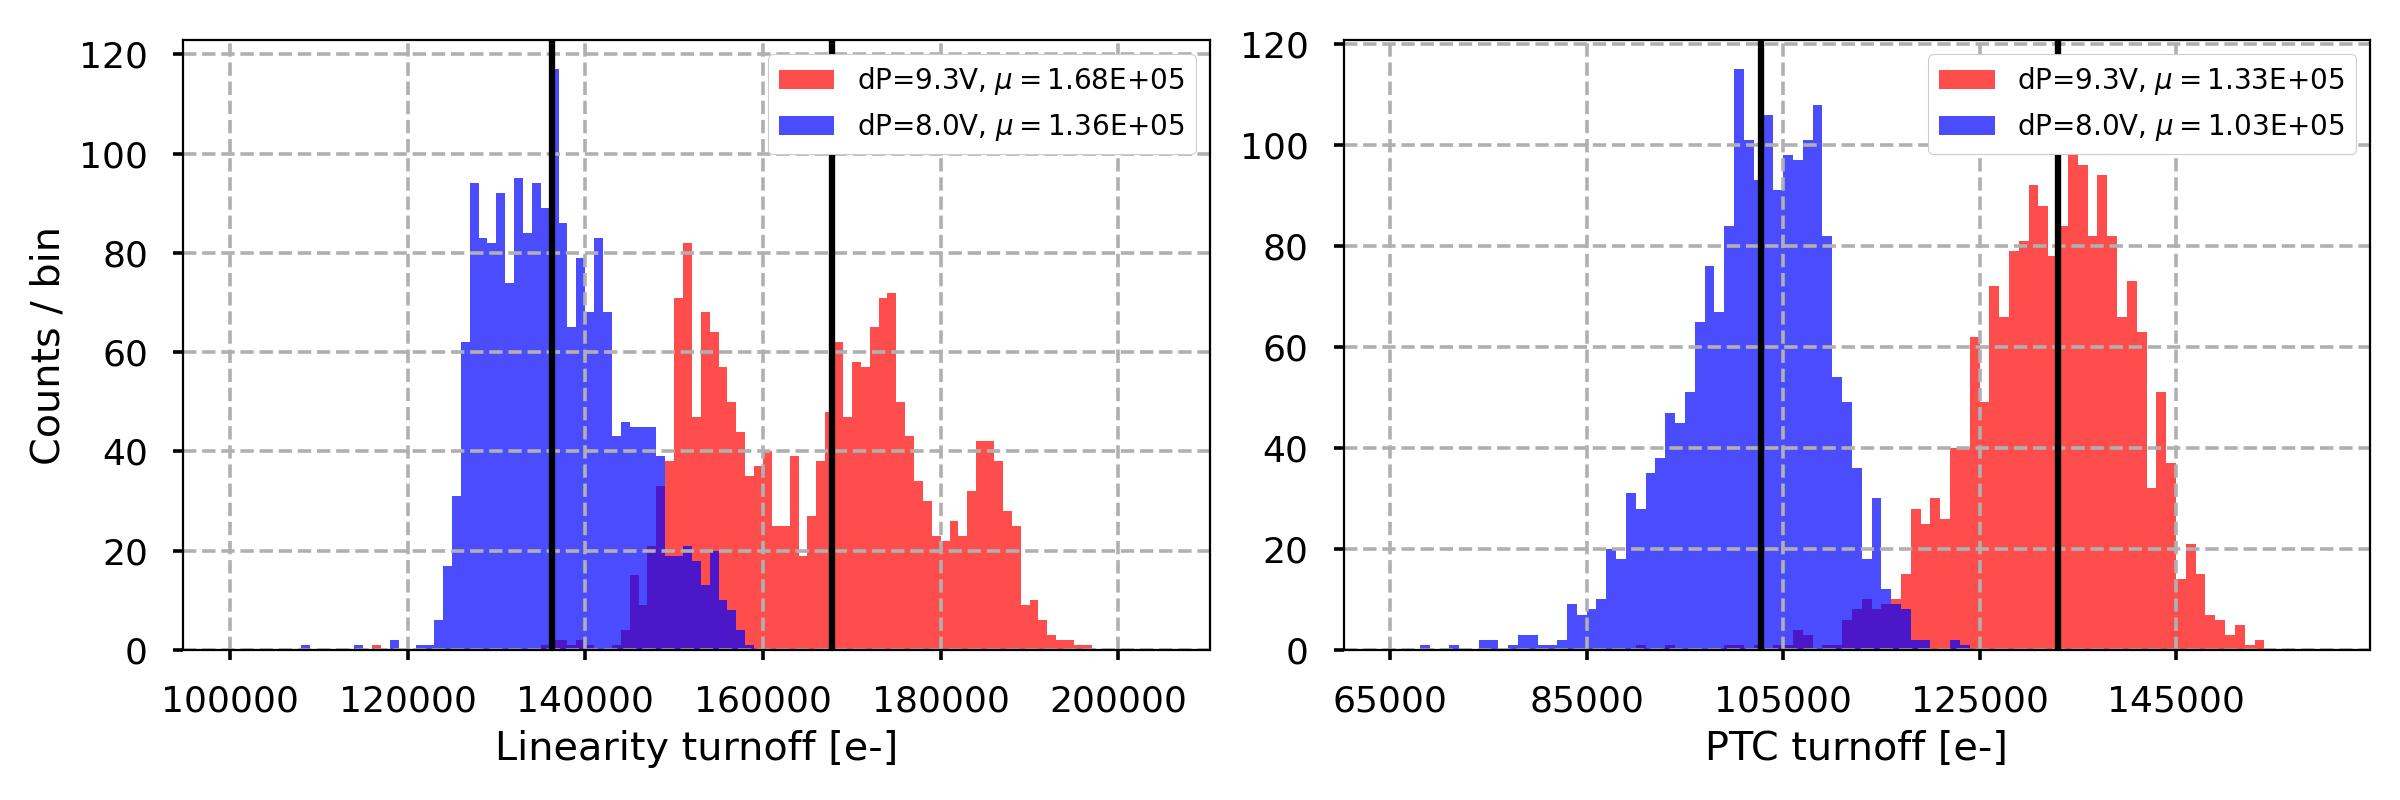
\includegraphics[width=0.7\linewidth]{figures/finalCharacterization/fullWellComparisons.jpg}
    \caption{Comparisons of (left) linearity turnoff and (right) PTC turnoff for e2v science sensors. The runs analyzed here are the PTC runs noted in Table~\ref{tab:runTable}. Note that both metrics have been gain corrected. Three peaks are observed for linearity turnoff for dP = 9.3\,V, and these resolve to one peak with a greater width for dP = 8.0\,V. A minor spatial correlation of linearity turnoff across the focal plane for the dP = 9.3\,V configuration is the primary source of this three-peak population.}
    \label{fig:finalChar-fullWell}
\end{figure}


\clearpage
\paragraph{PTC Gain}\label{final-ptc-gain}

PTC gain was evaluated from the PTC runs (Fig.~\ref{fig:finalChar-PTCGain-5x5}. PTC gain values are quite similar for the initial and final Run 7 runs, with a minor increase in gain observed in e2v sensors (Fig.~\ref{fig:finalChar-PTCGain_HistComp}).

\begin{figure}[ht]
    \centering
    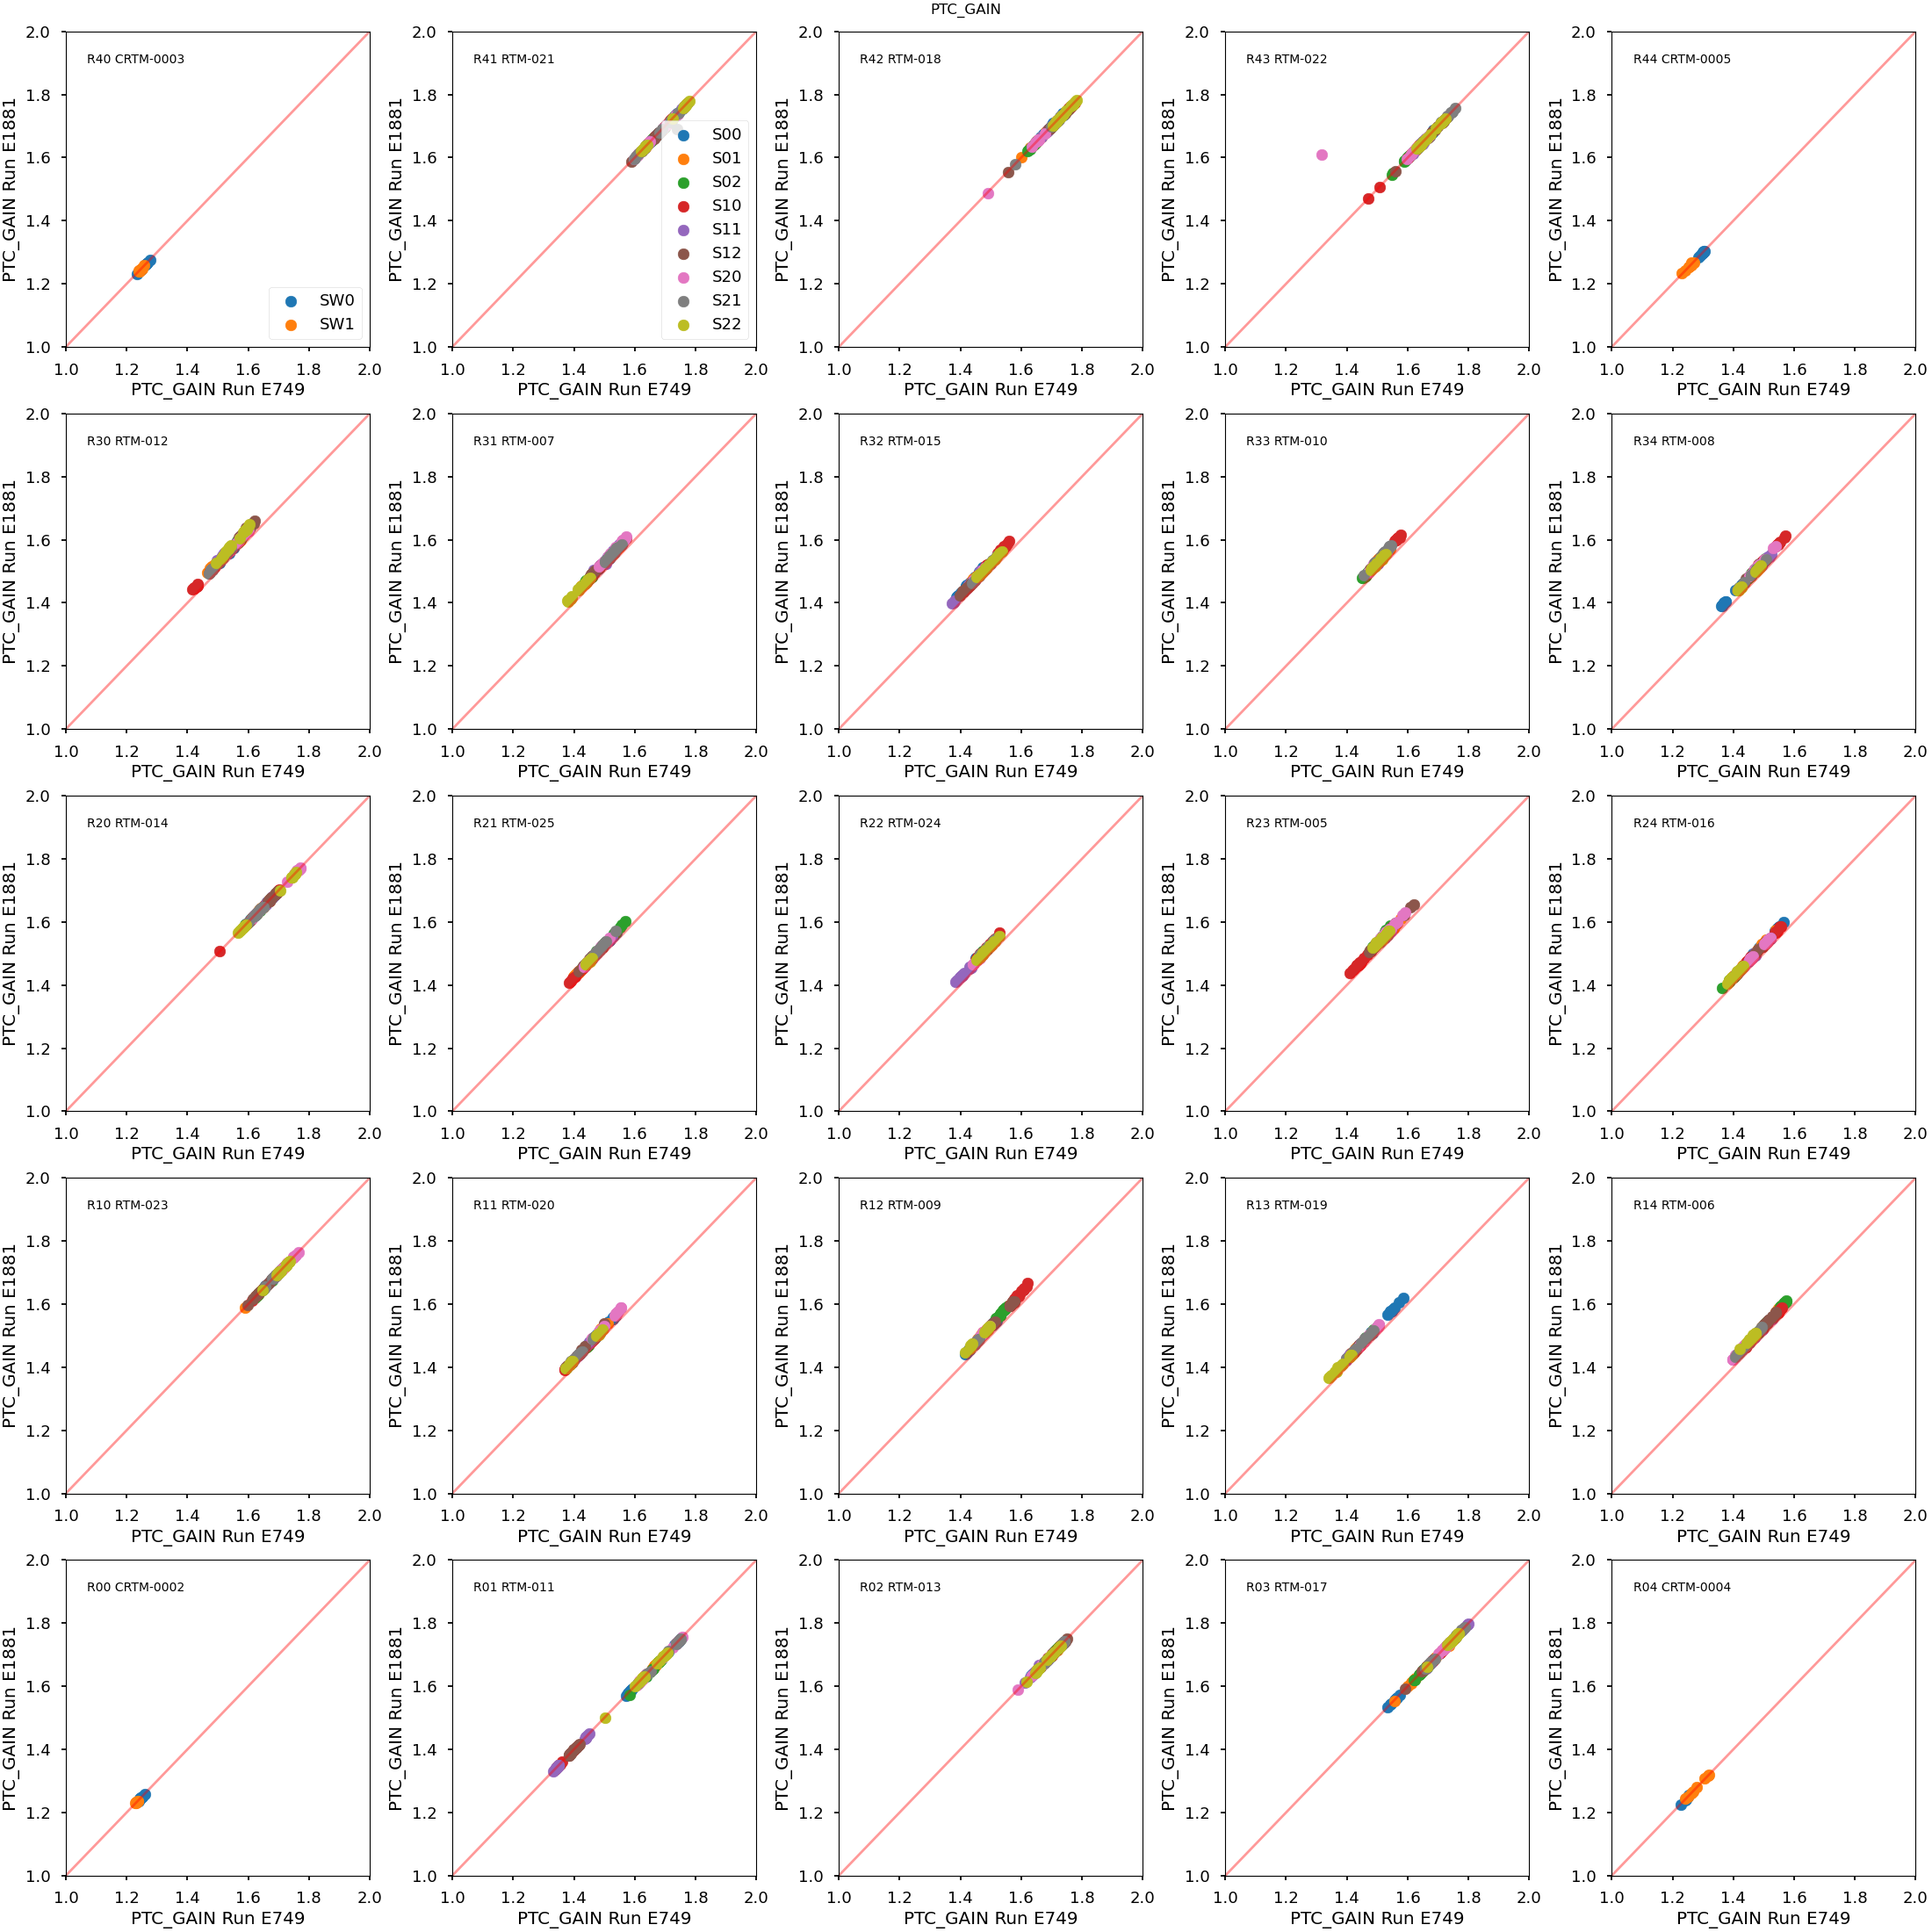
\includegraphics[width=0.7\linewidth]{figures/finalCharacterization/E749_E1881_PTC_GAIN.png}
    \caption{Comparison of PTC gain amplifier measurements.  The consistence between initial and final Run 7 values is quite good.}
    \label{fig:finalChar-PTCGain-5x5}
\end{figure}

The magnitude of the gain increase for e2v sensors in the final Run 7 configuration is \textasciitilde0.03 e-/ADU on average.

\begin{figure}[ht]
    \centering
    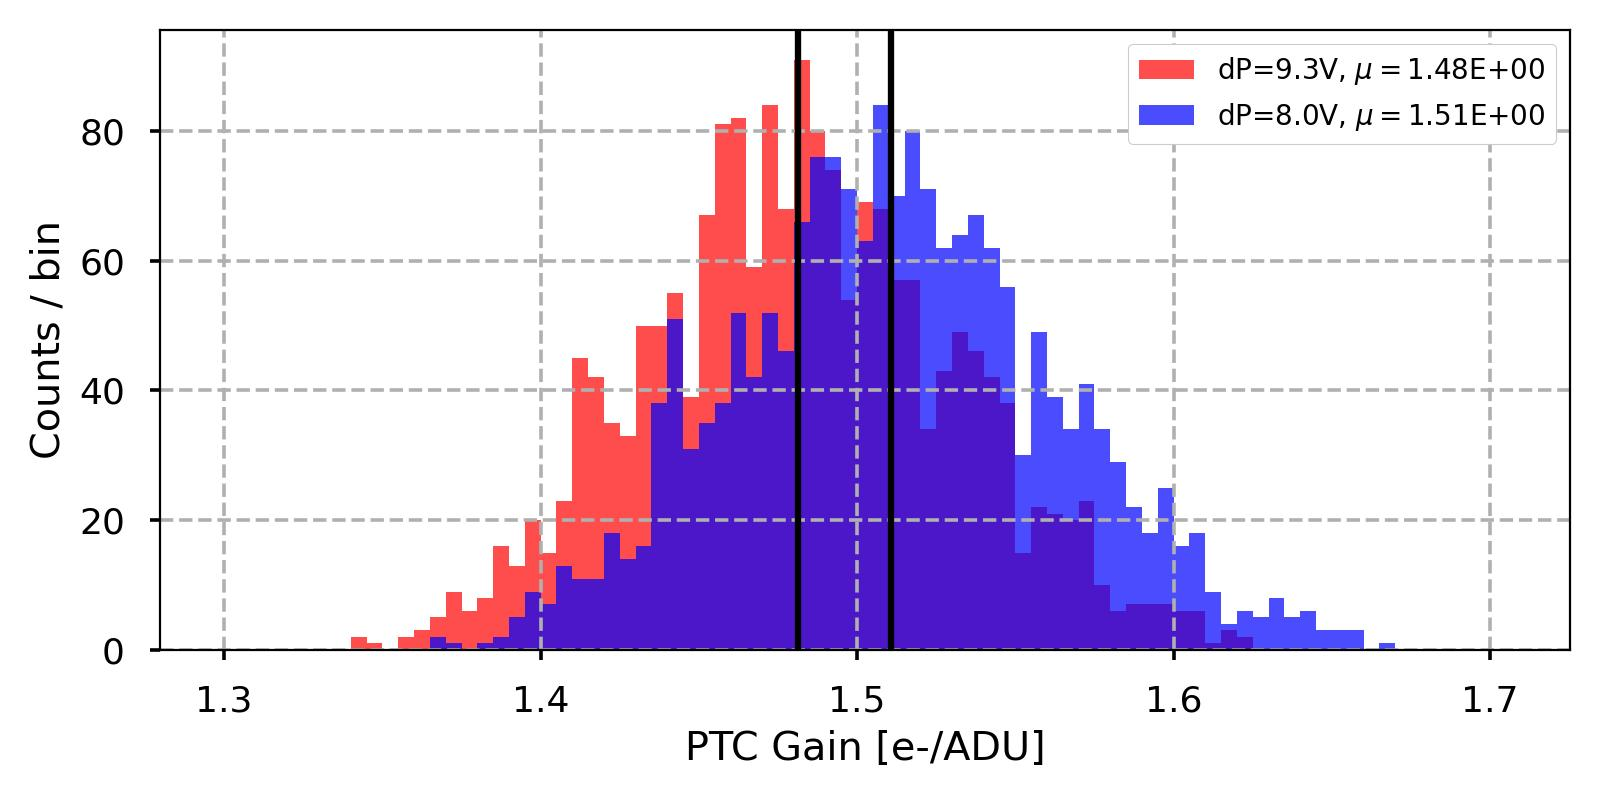
\includegraphics[width=0.7\linewidth]{figures/finalCharacterization/PTCGainComp.jpg}
    \caption{Comparison of PTC gains for e2v science sensors, with a moderate increase in the final run condition. The black lines denote the median value for each population of measurements, shown in the legend.}
    \label{fig:finalChar-PTCGain_HistComp}
\end{figure}

\clearpage

\paragraph{Read Noise}\label{sec:finalChar:ReadNoise}

The read noise is found to be consistent for both e2v and ITL sensors between the initial and final Run 7 conditions (Fig.~\ref{fig:finalChar-READNoise}). R01\_S02 shows lower read noise in the final Run 7 configuration. R01\_S02 is a known problem sensor with high read noise (see Section~\ref{deadamplifiers}), so improvement in this regime is a welcome sign.

\begin{figure}[ht]
    \centering
    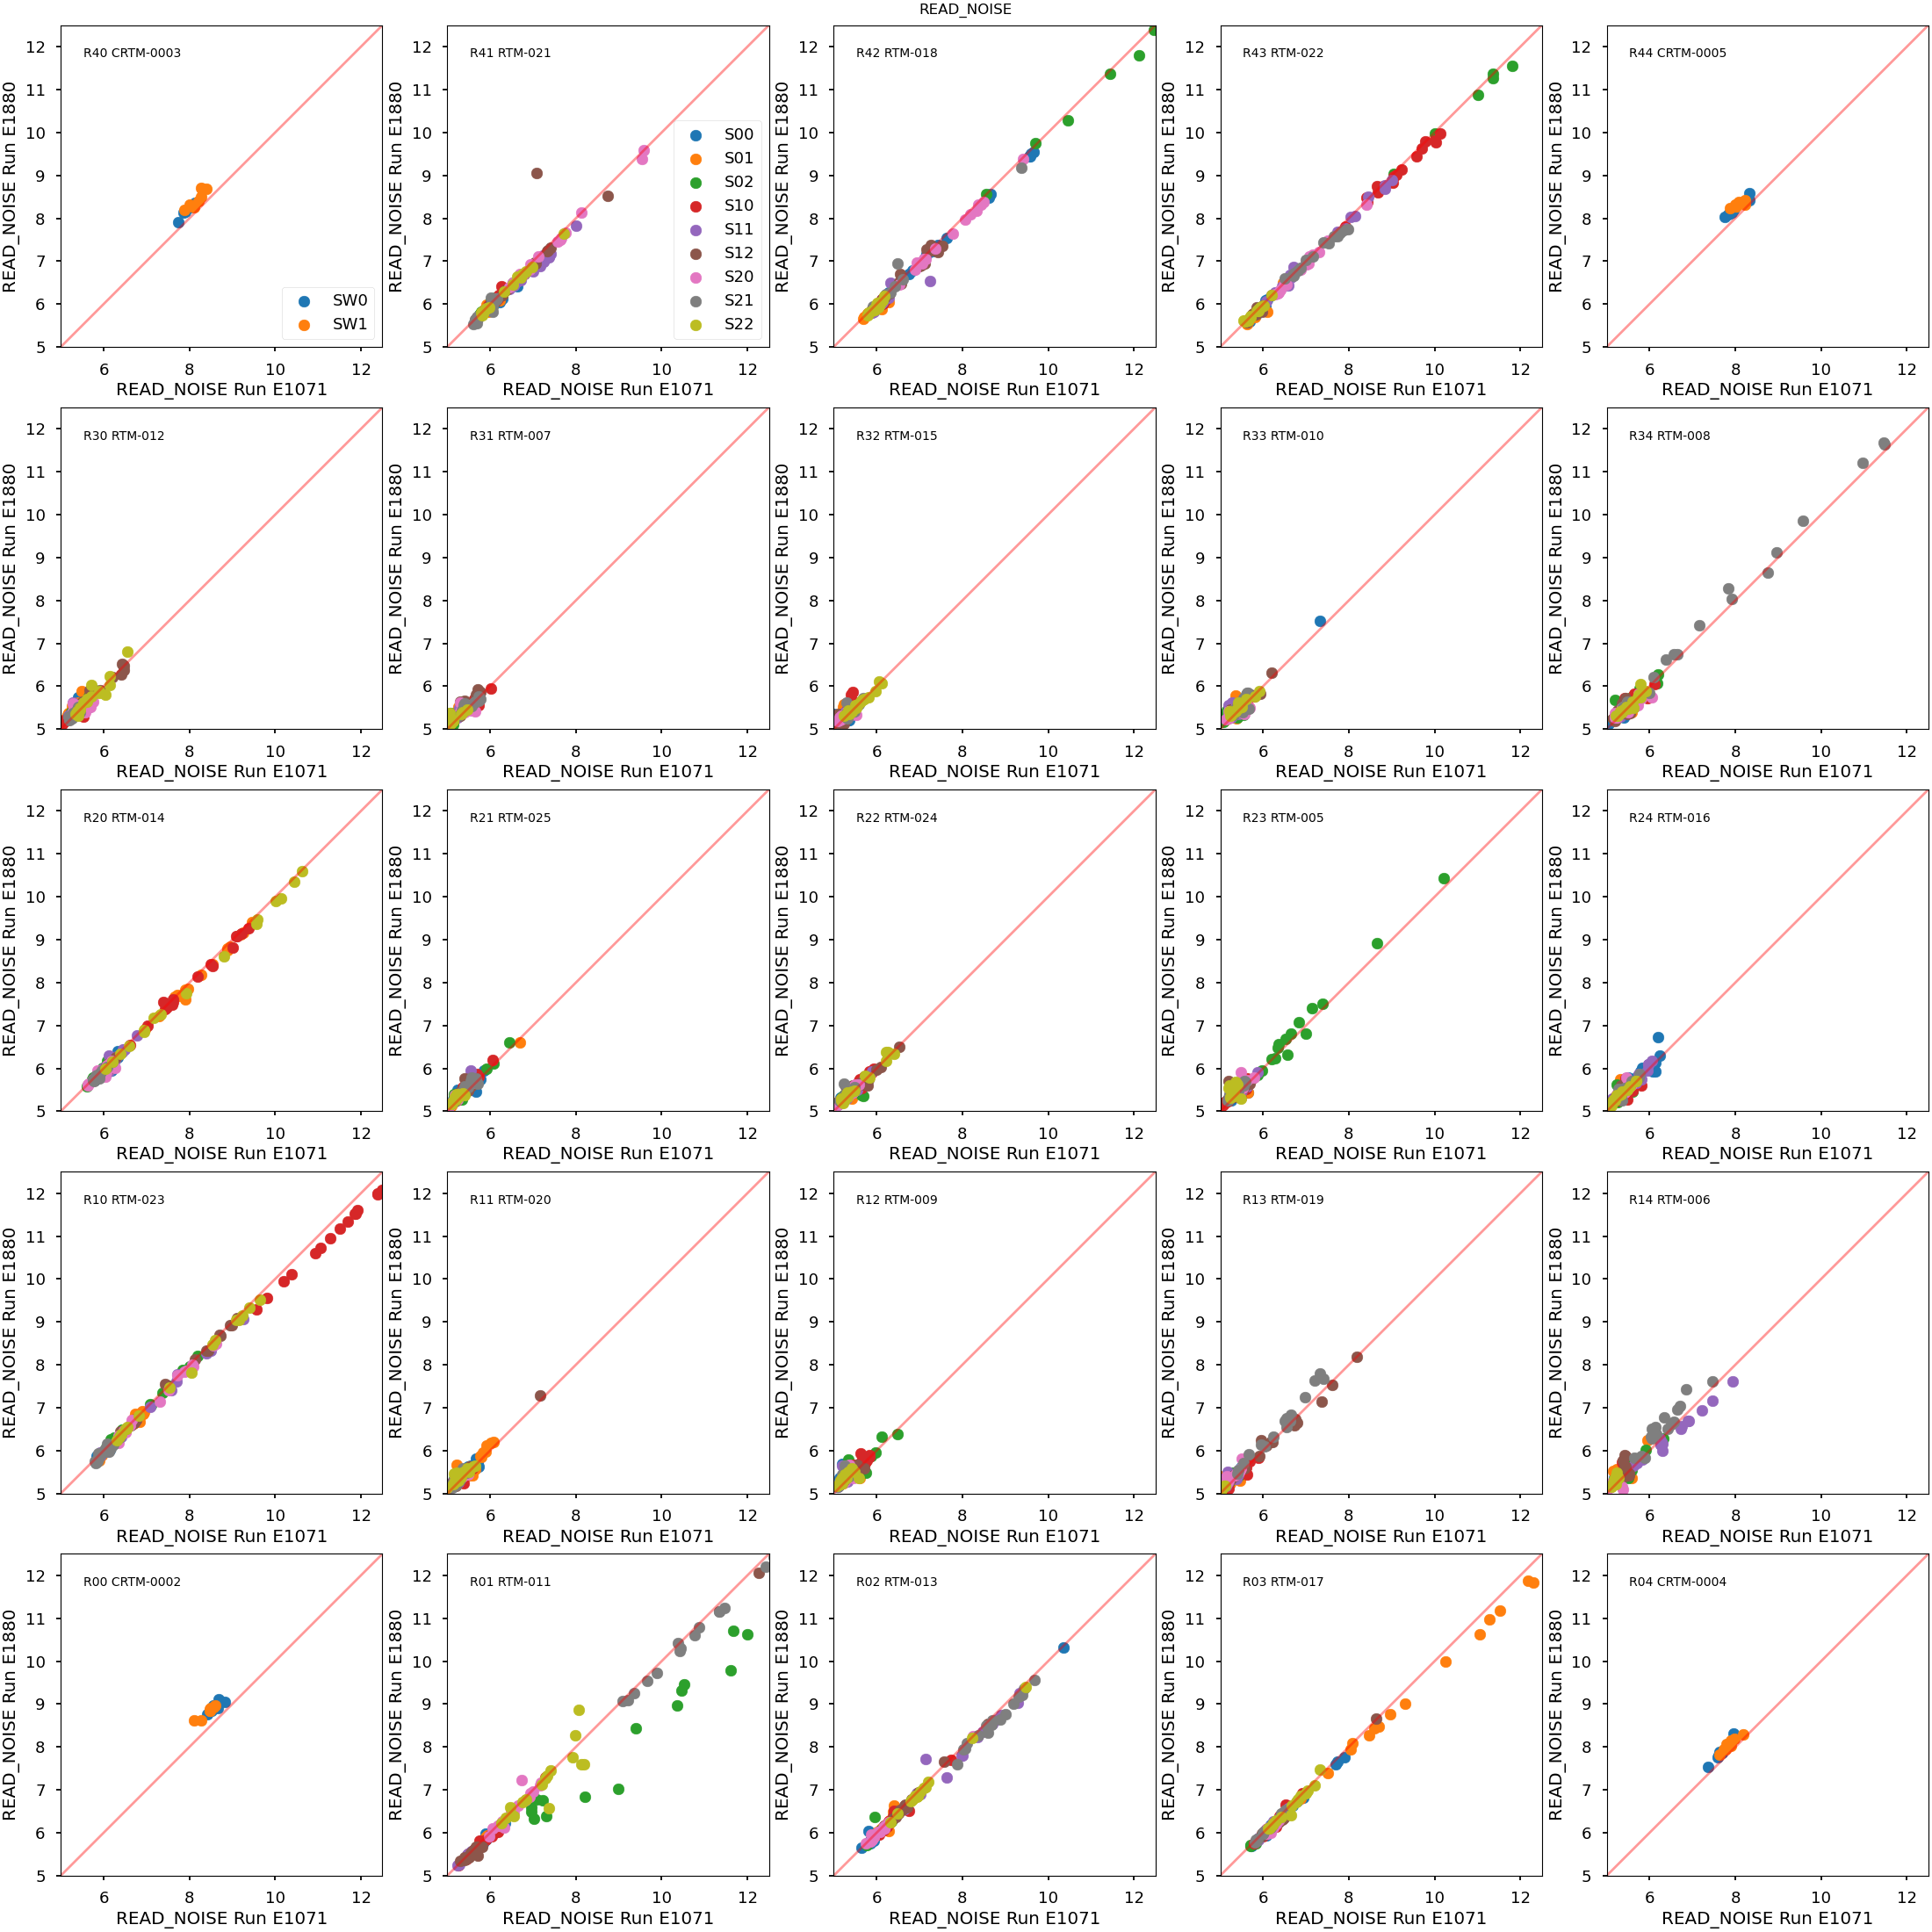
\includegraphics[width=0.7\linewidth]{figures/finalCharacterization/E1071_E1880_READ_NOISE_inset.png}
    \caption{Comparison of read noise measurements for initial and final Run 7 conditions.}
    \label{fig:finalChar-READNoise}
\end{figure}

The read noise measured for both sensor types differs by $\lesssim 0.1$ e- on average between the runs (Fig.~\ref{fig:finalChar:ReadNoiseByManu}).

\begin{figure}[ht]
    \centering
    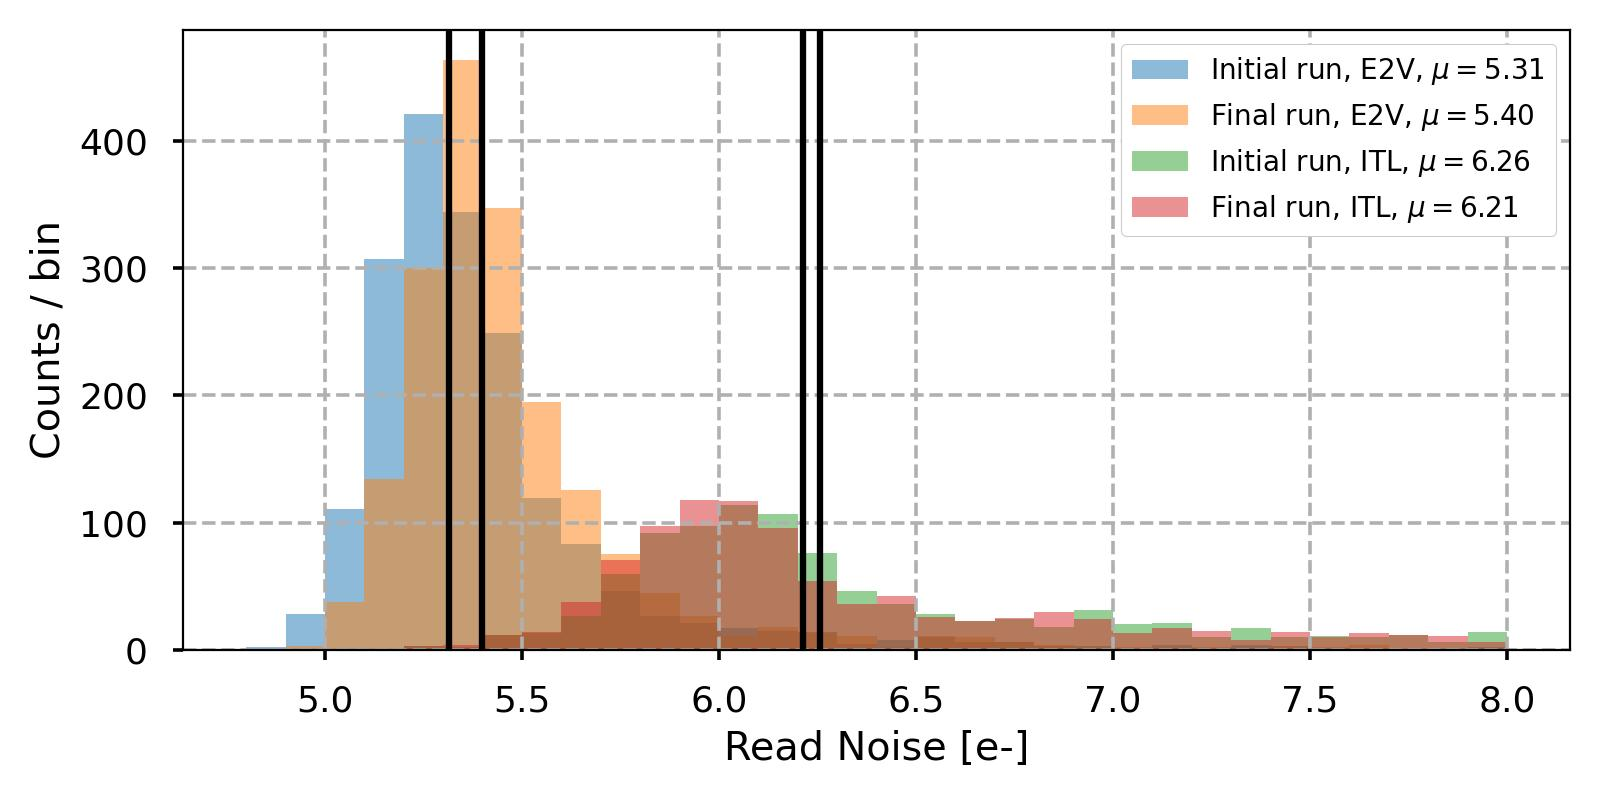
\includegraphics[width=0.7\linewidth]{figures/finalCharacterization/ReadNoiseComp.jpg}
    \caption{Comparison of the read noise measurements in e2v and ITL sensors for the initial and final Run 7 runs.}
    \label{fig:finalChar:ReadNoiseByManu}
\end{figure}

\paragraph{PTC Noise}\label{sec:finalChar:PTCNoise}

PTC noise is consistent between the initial and final Run 7 configurations (Fig.~\ref{fig:finalChar-PTC_noise_5x5}). No significant deviation in measurements is observed.

\begin{figure}[ht]
    \centering
    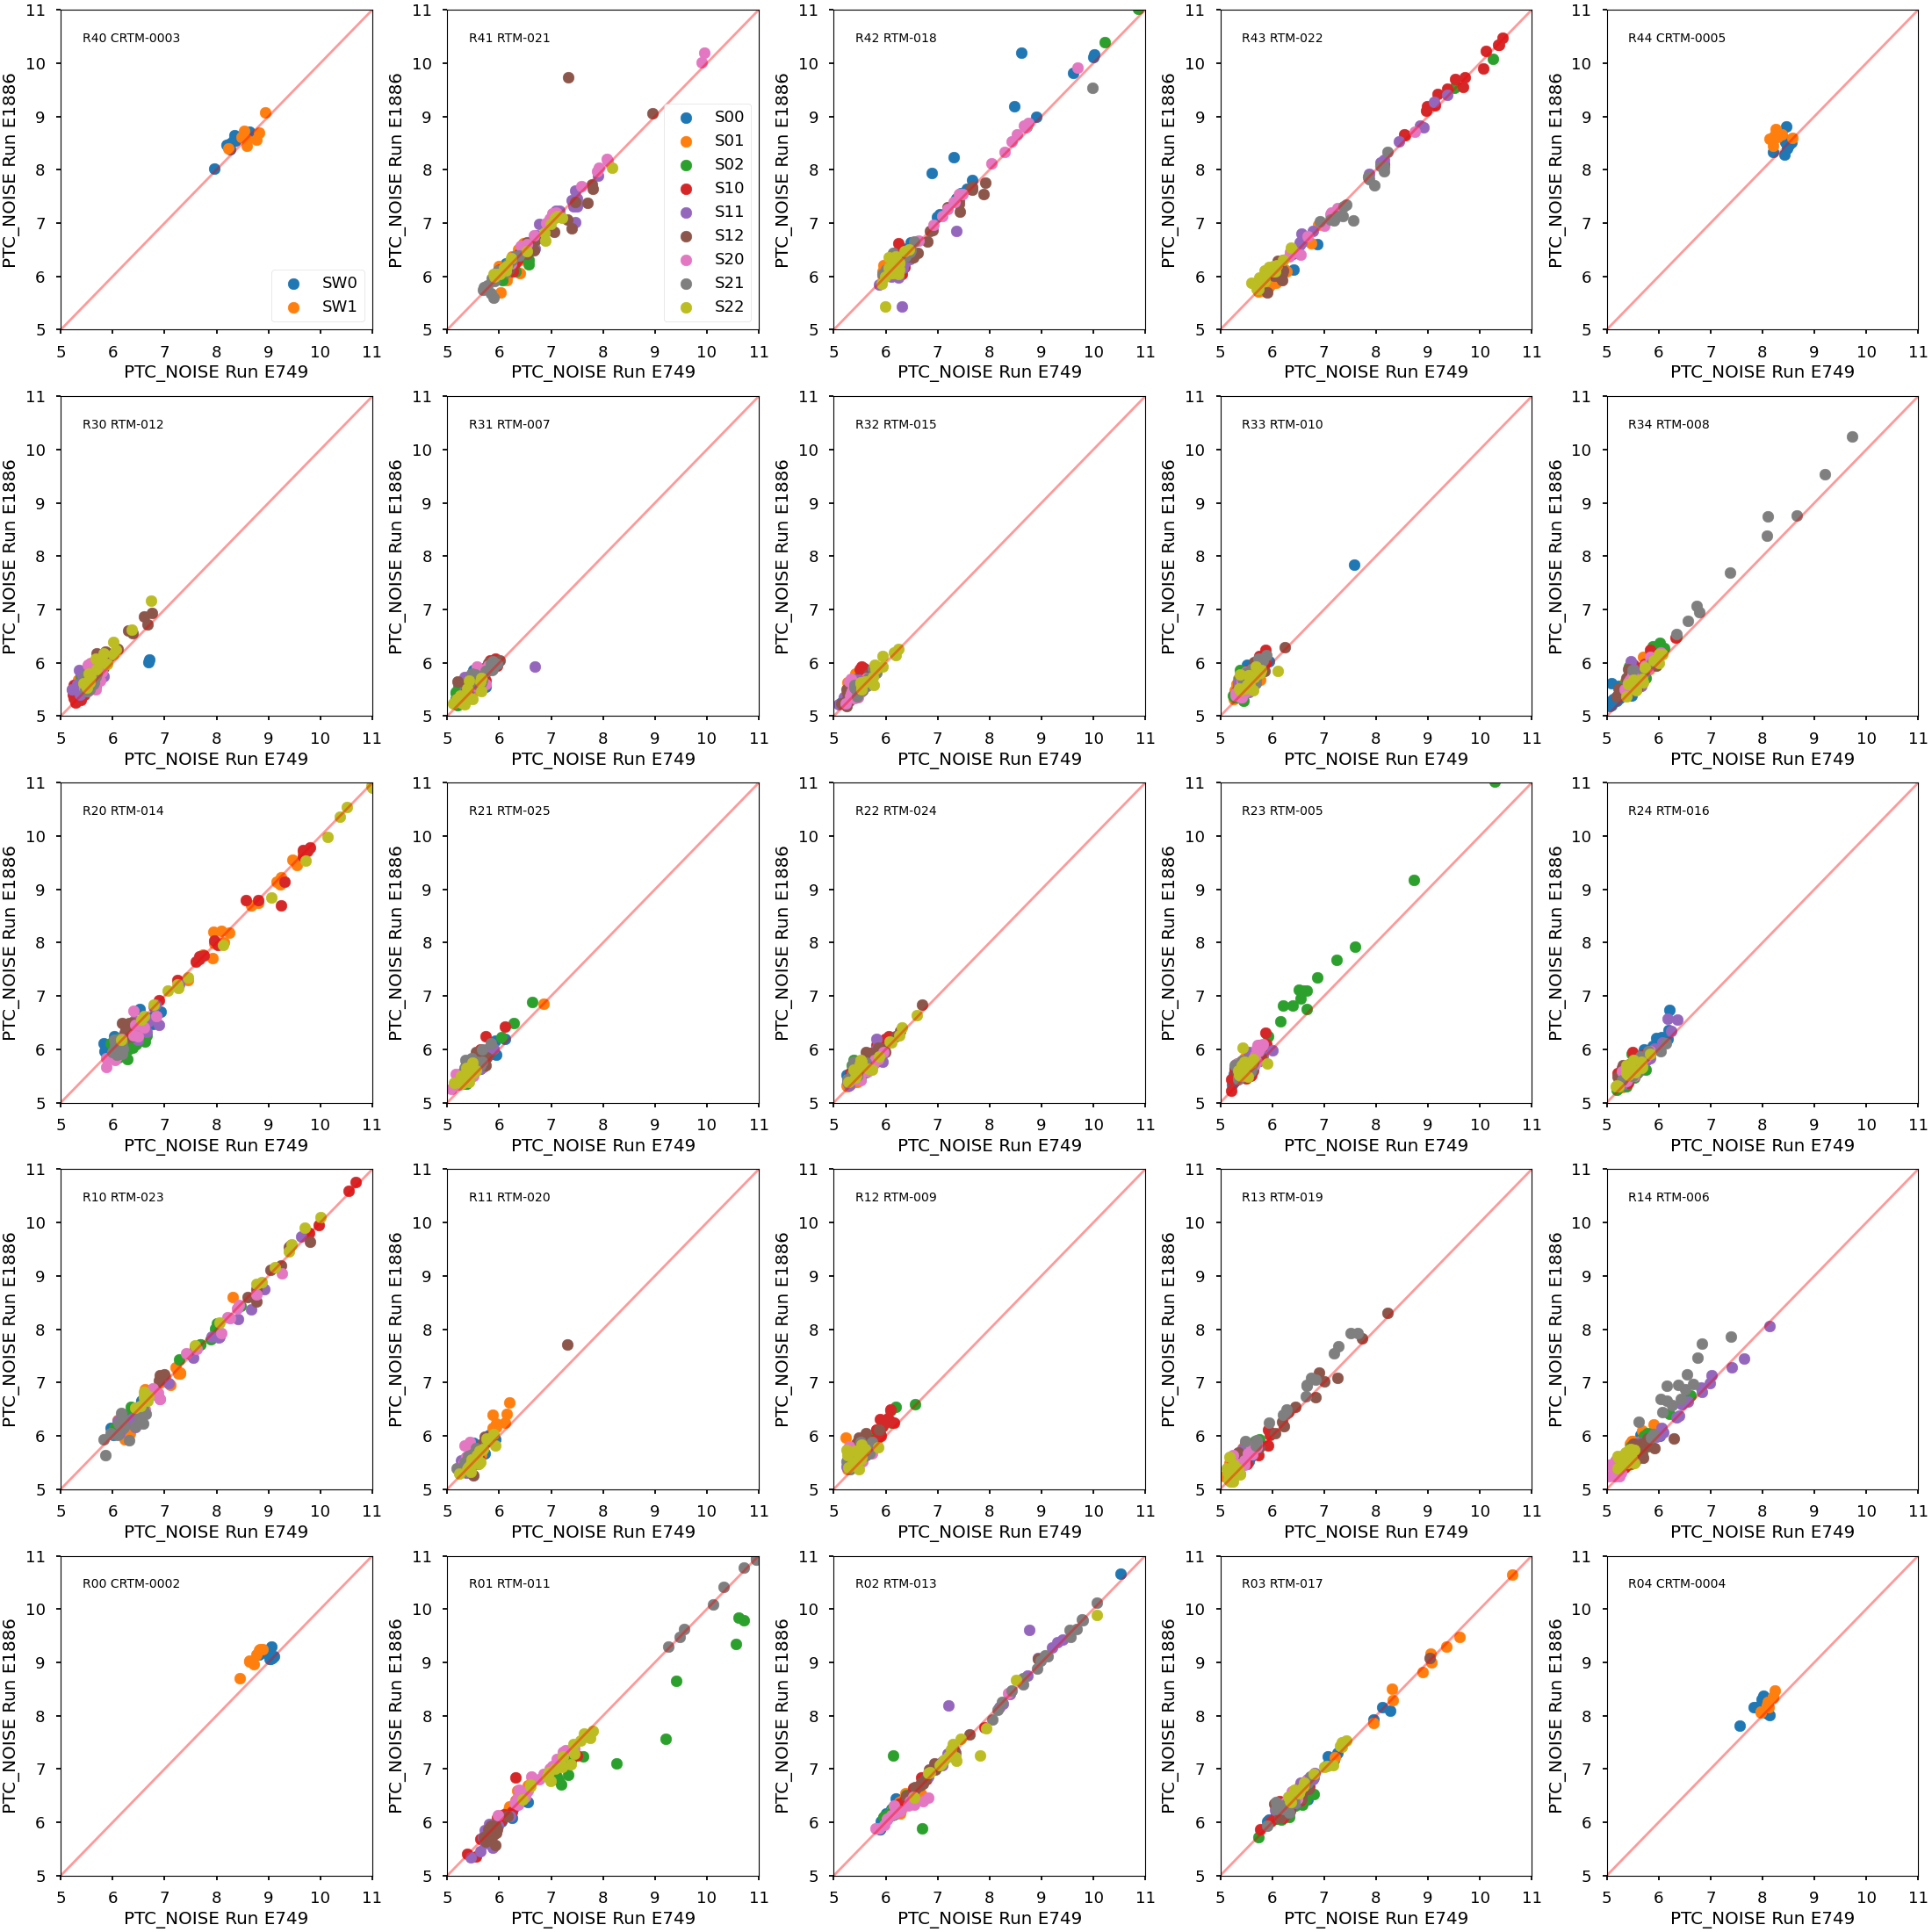
\includegraphics[width=0.7\linewidth]{figures/finalCharacterization/E749_E1886_PTC_NOISE.png}
    \caption{Comparison of PTC noise measurements for initial and final Run 7 conditions.}
    \label{fig:finalChar-PTC_noise_5x5}
\end{figure}

The average deviation of PTC noise measurements between initial and final runs is $\lesssim$ 0.1 e- for both e2v and ITL detector types, with no significant biases emerging (Fig.~\ref{fig:finalChar:PTCNoise_diff_hist}).

\begin{figure}[ht]
    \centering
    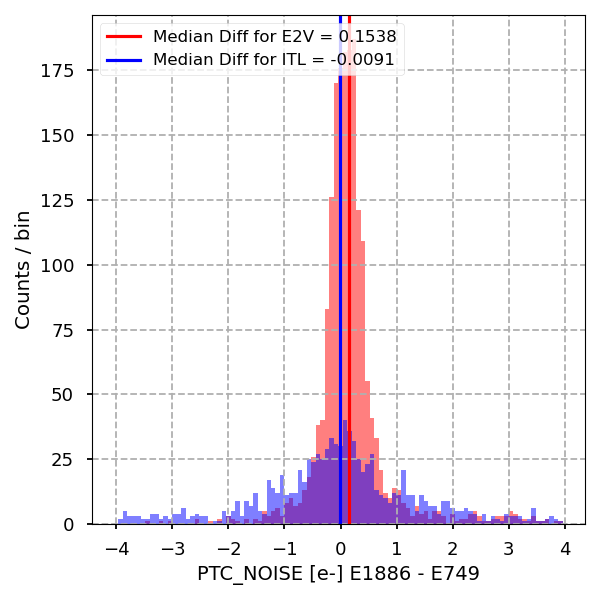
\includegraphics[width=0.7\linewidth]{figures/finalCharacterization/PTC_NOISE_E749_E1886_diff.png}
    \caption{Comparison of the PTC noise measurements in e2v and ITL sensors for the initial and final Run 7 runs.}
    \label{fig:finalChar:PTCNoise_diff_hist}
\end{figure}

\paragraph{Brighter-fatter $a_{00}$ coefficient}\label{final-brighter-fatter-a00-coefficient}

The principle area change component closely related to the brighter-fatter effect, quantified by $a_{00}$ following the model of \cite{2019A&A...629A..36A}, is modified in the final Run 7 operating conditions by the lower parallel swing for e2v sensors. We observe an extremely high consistency for ITL sensors (Fig.~\ref{fig:finalChar-PTC_A00_5x5}).

\begin{figure}[ht]
    \centering
    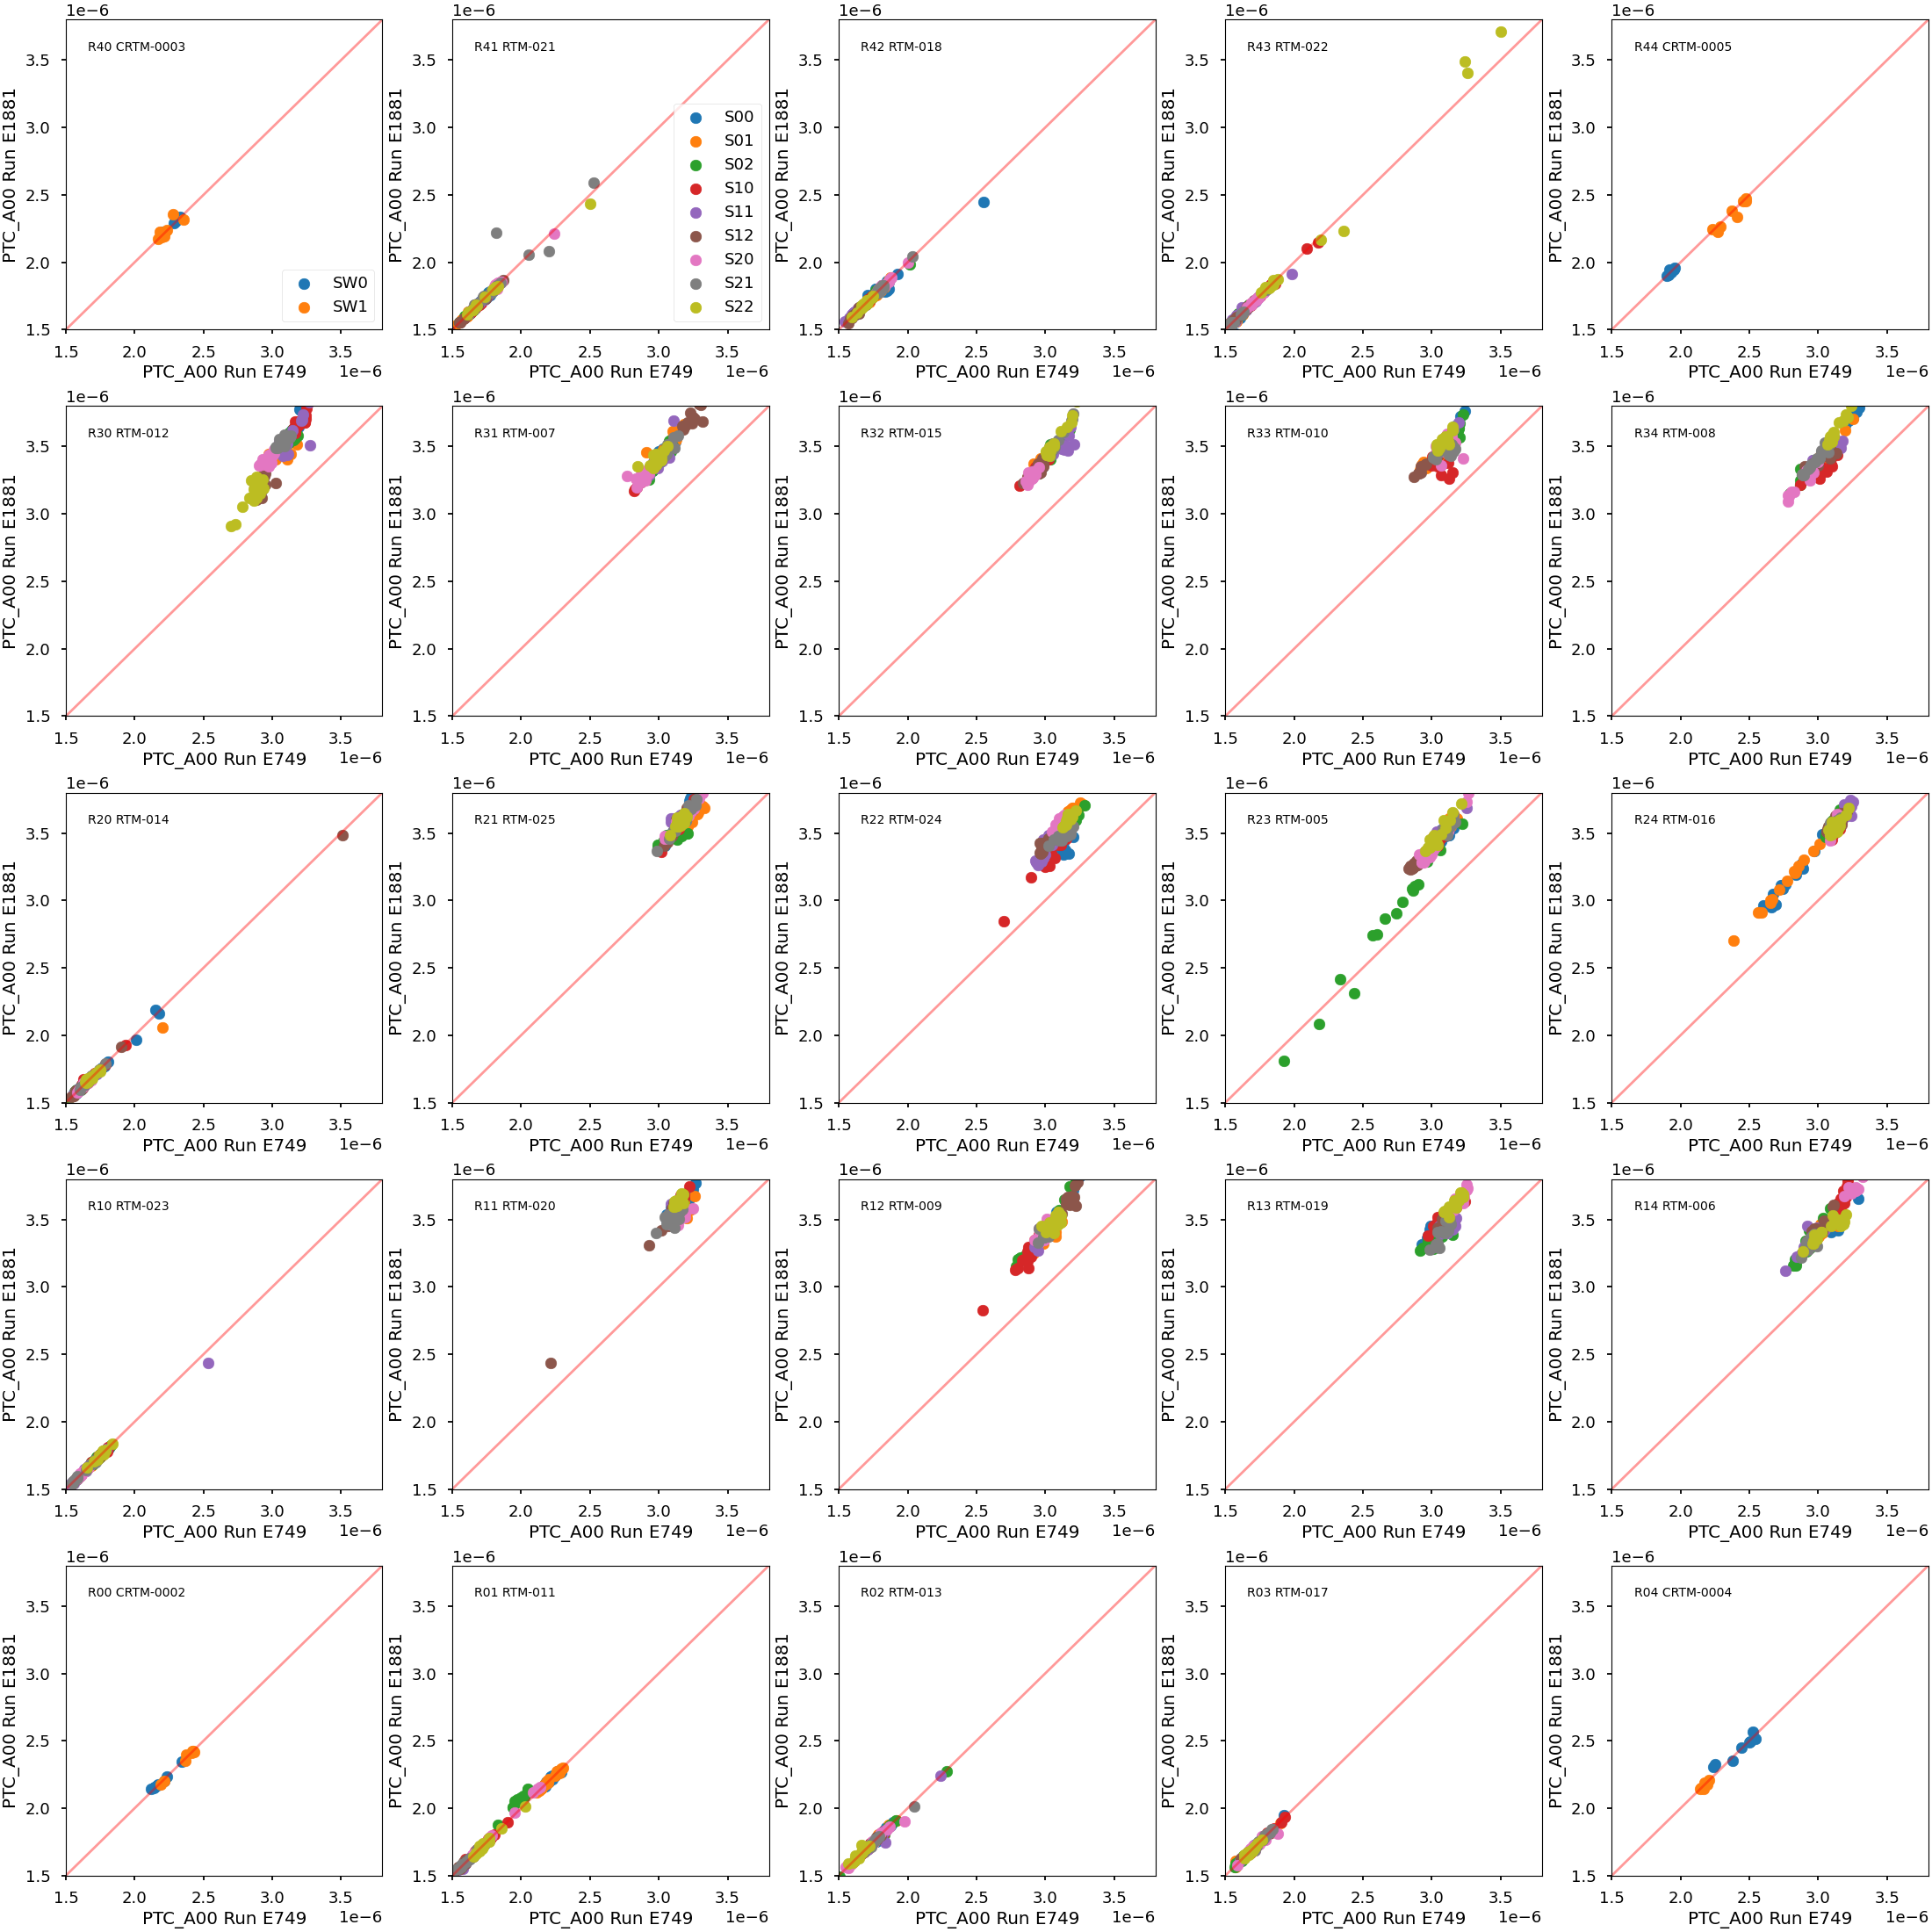
\includegraphics[width=0.7\linewidth]{figures/finalCharacterization/E749_E1881_PTC_A00.png}
    \caption{Comparison of per-amplifier measurements of the $a_{00}$ parameter for initial and final Run 7 conditions.}
    \label{fig:finalChar-PTC_A00_5x5}
\end{figure}

The change in the $a_{00}$ value for e2v sensors is illustrated in Figure~\ref{fig:finalChar-PTC_A00_E2VComp}, showing a \textasciitilde12\% increase in the strength of the brighter-fatter effect for e2v sensors due to the lower parallel swing. For additional discussion of the brighter-fatter coefficient, see Section~\ref{impact-on-brighter-fatter-effect}.

\begin{figure}[ht]
    \centering
    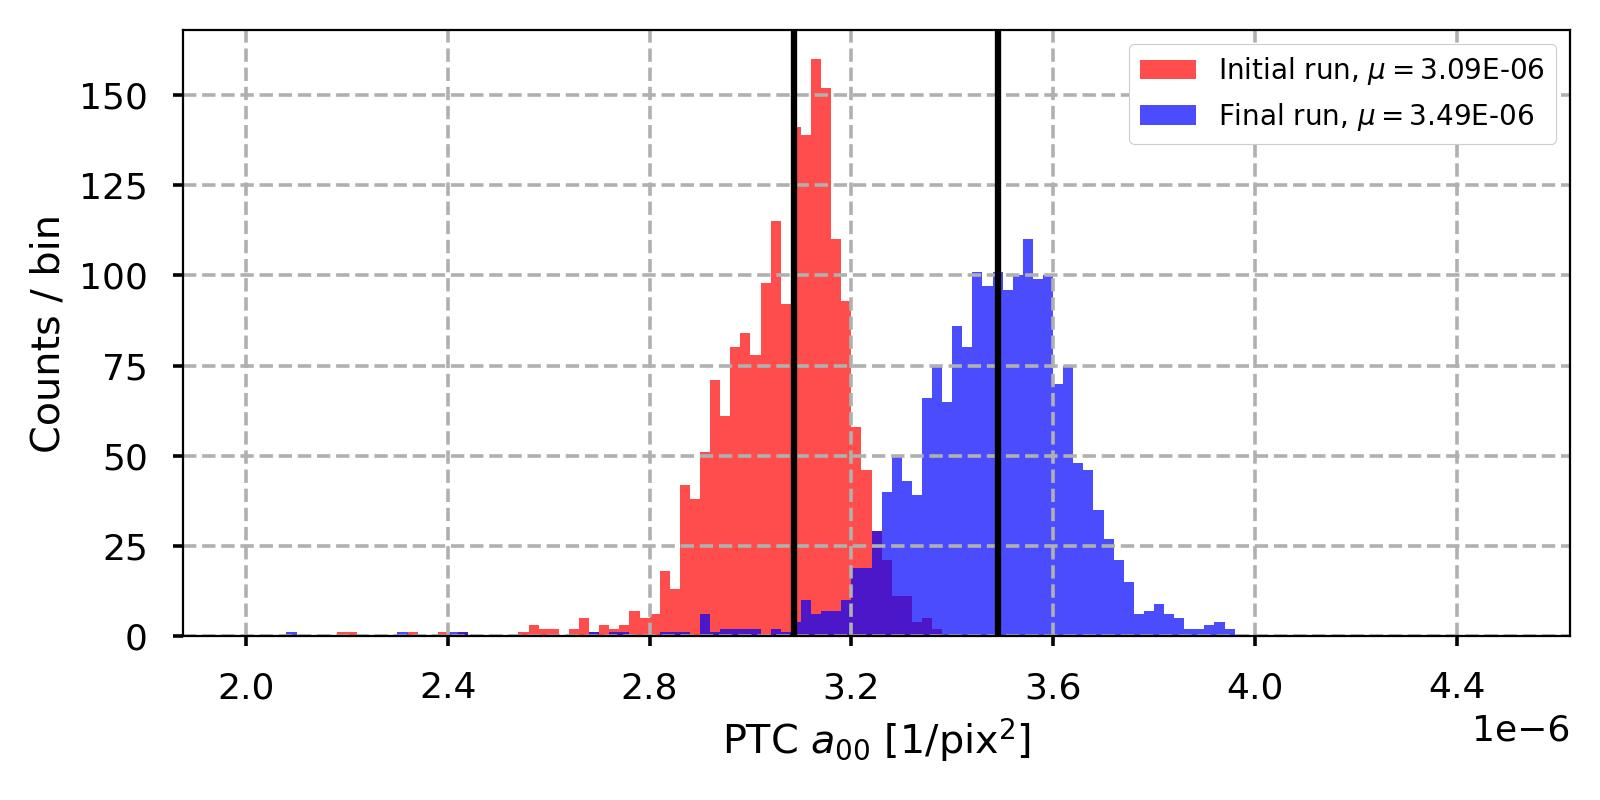
\includegraphics[width=0.7\linewidth]{figures/finalCharacterization/PTCA00Comp.jpg}
    \caption{Comparison of the $a_{00}$ values in e2v sensors, showing a notable increase in the final operating conditions.  As noted in the legend, the vertical black lines indicate the median values of the respective distributions.}
    \label{fig:finalChar-PTC_A00_E2VComp}
\end{figure}

\clearpage
\paragraph{Brighter-Fatter Correlation}\label{final-brighter-fatter-correlation}

The strength of the brighter-fatter correlations  were extracted from the PTC runs. For both x and y correlations, the results are quite consistent across initial and final Run 7 operating conditions (Figs.~\ref{fig:finalChar-BFXCorr-5x5} and \ref{fig:finalChar-BFYCorr-5x5}).

\begin{figure}[ht]
    \centering
    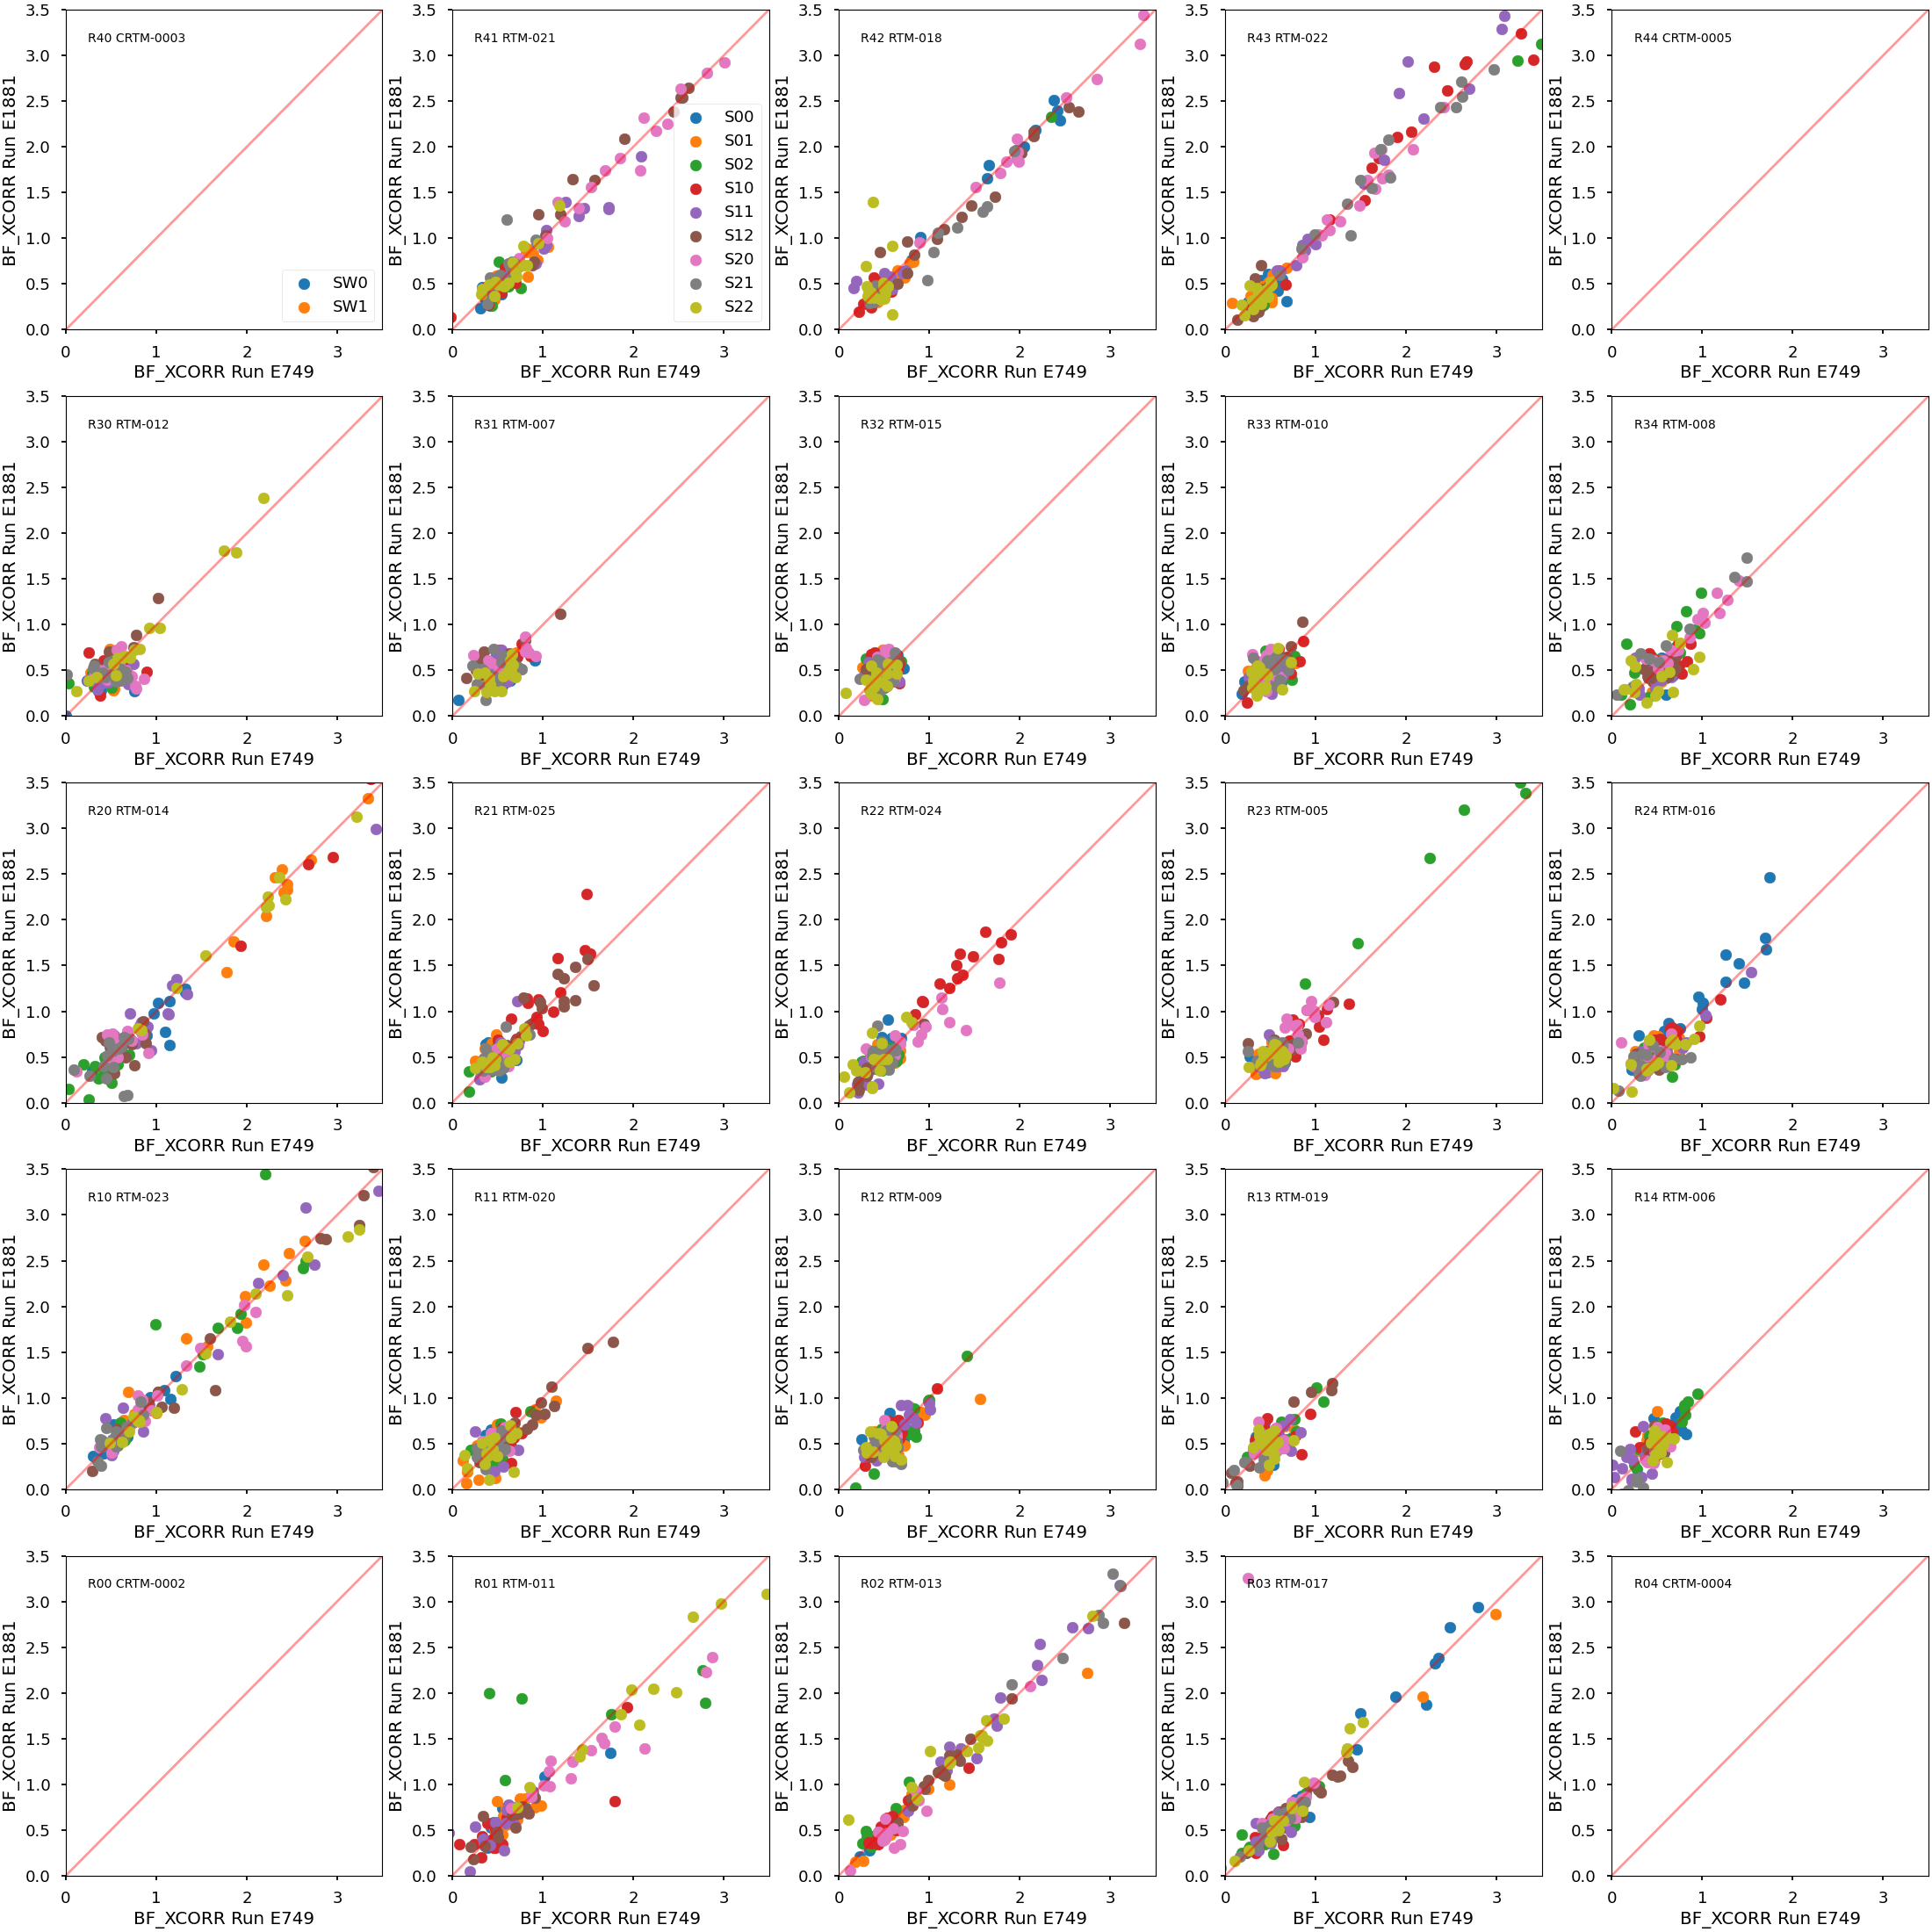
\includegraphics[width=0.7\linewidth]{figures/finalCharacterization/E749_E1881_BF_XCORR.png}
    \caption{Comparison of per-amplifier measurements of the brighter-fatter x-correlation for initial and final Run 7 conditions. For the corner rafts, the correlations are outside of the ranges shown here.}
    \label{fig:finalChar-BFXCorr-5x5}
\end{figure}

Both correlations vary by \lesssim 2.2\% on average, decreasing in both instances for the final Run 7 configuration (Table~\ref{table:FinalChar-paramTable}). The measurement is noisy, with all rafts showing unbiased scatter around the correlation measurement on the raft level. %, as evident in Figures~\ref{fig:finalChar-BFXCorr-5x5} and \ref{fig:finalChar-BFYCorr-5x5}.

\begin{figure}[ht]
    \centering
    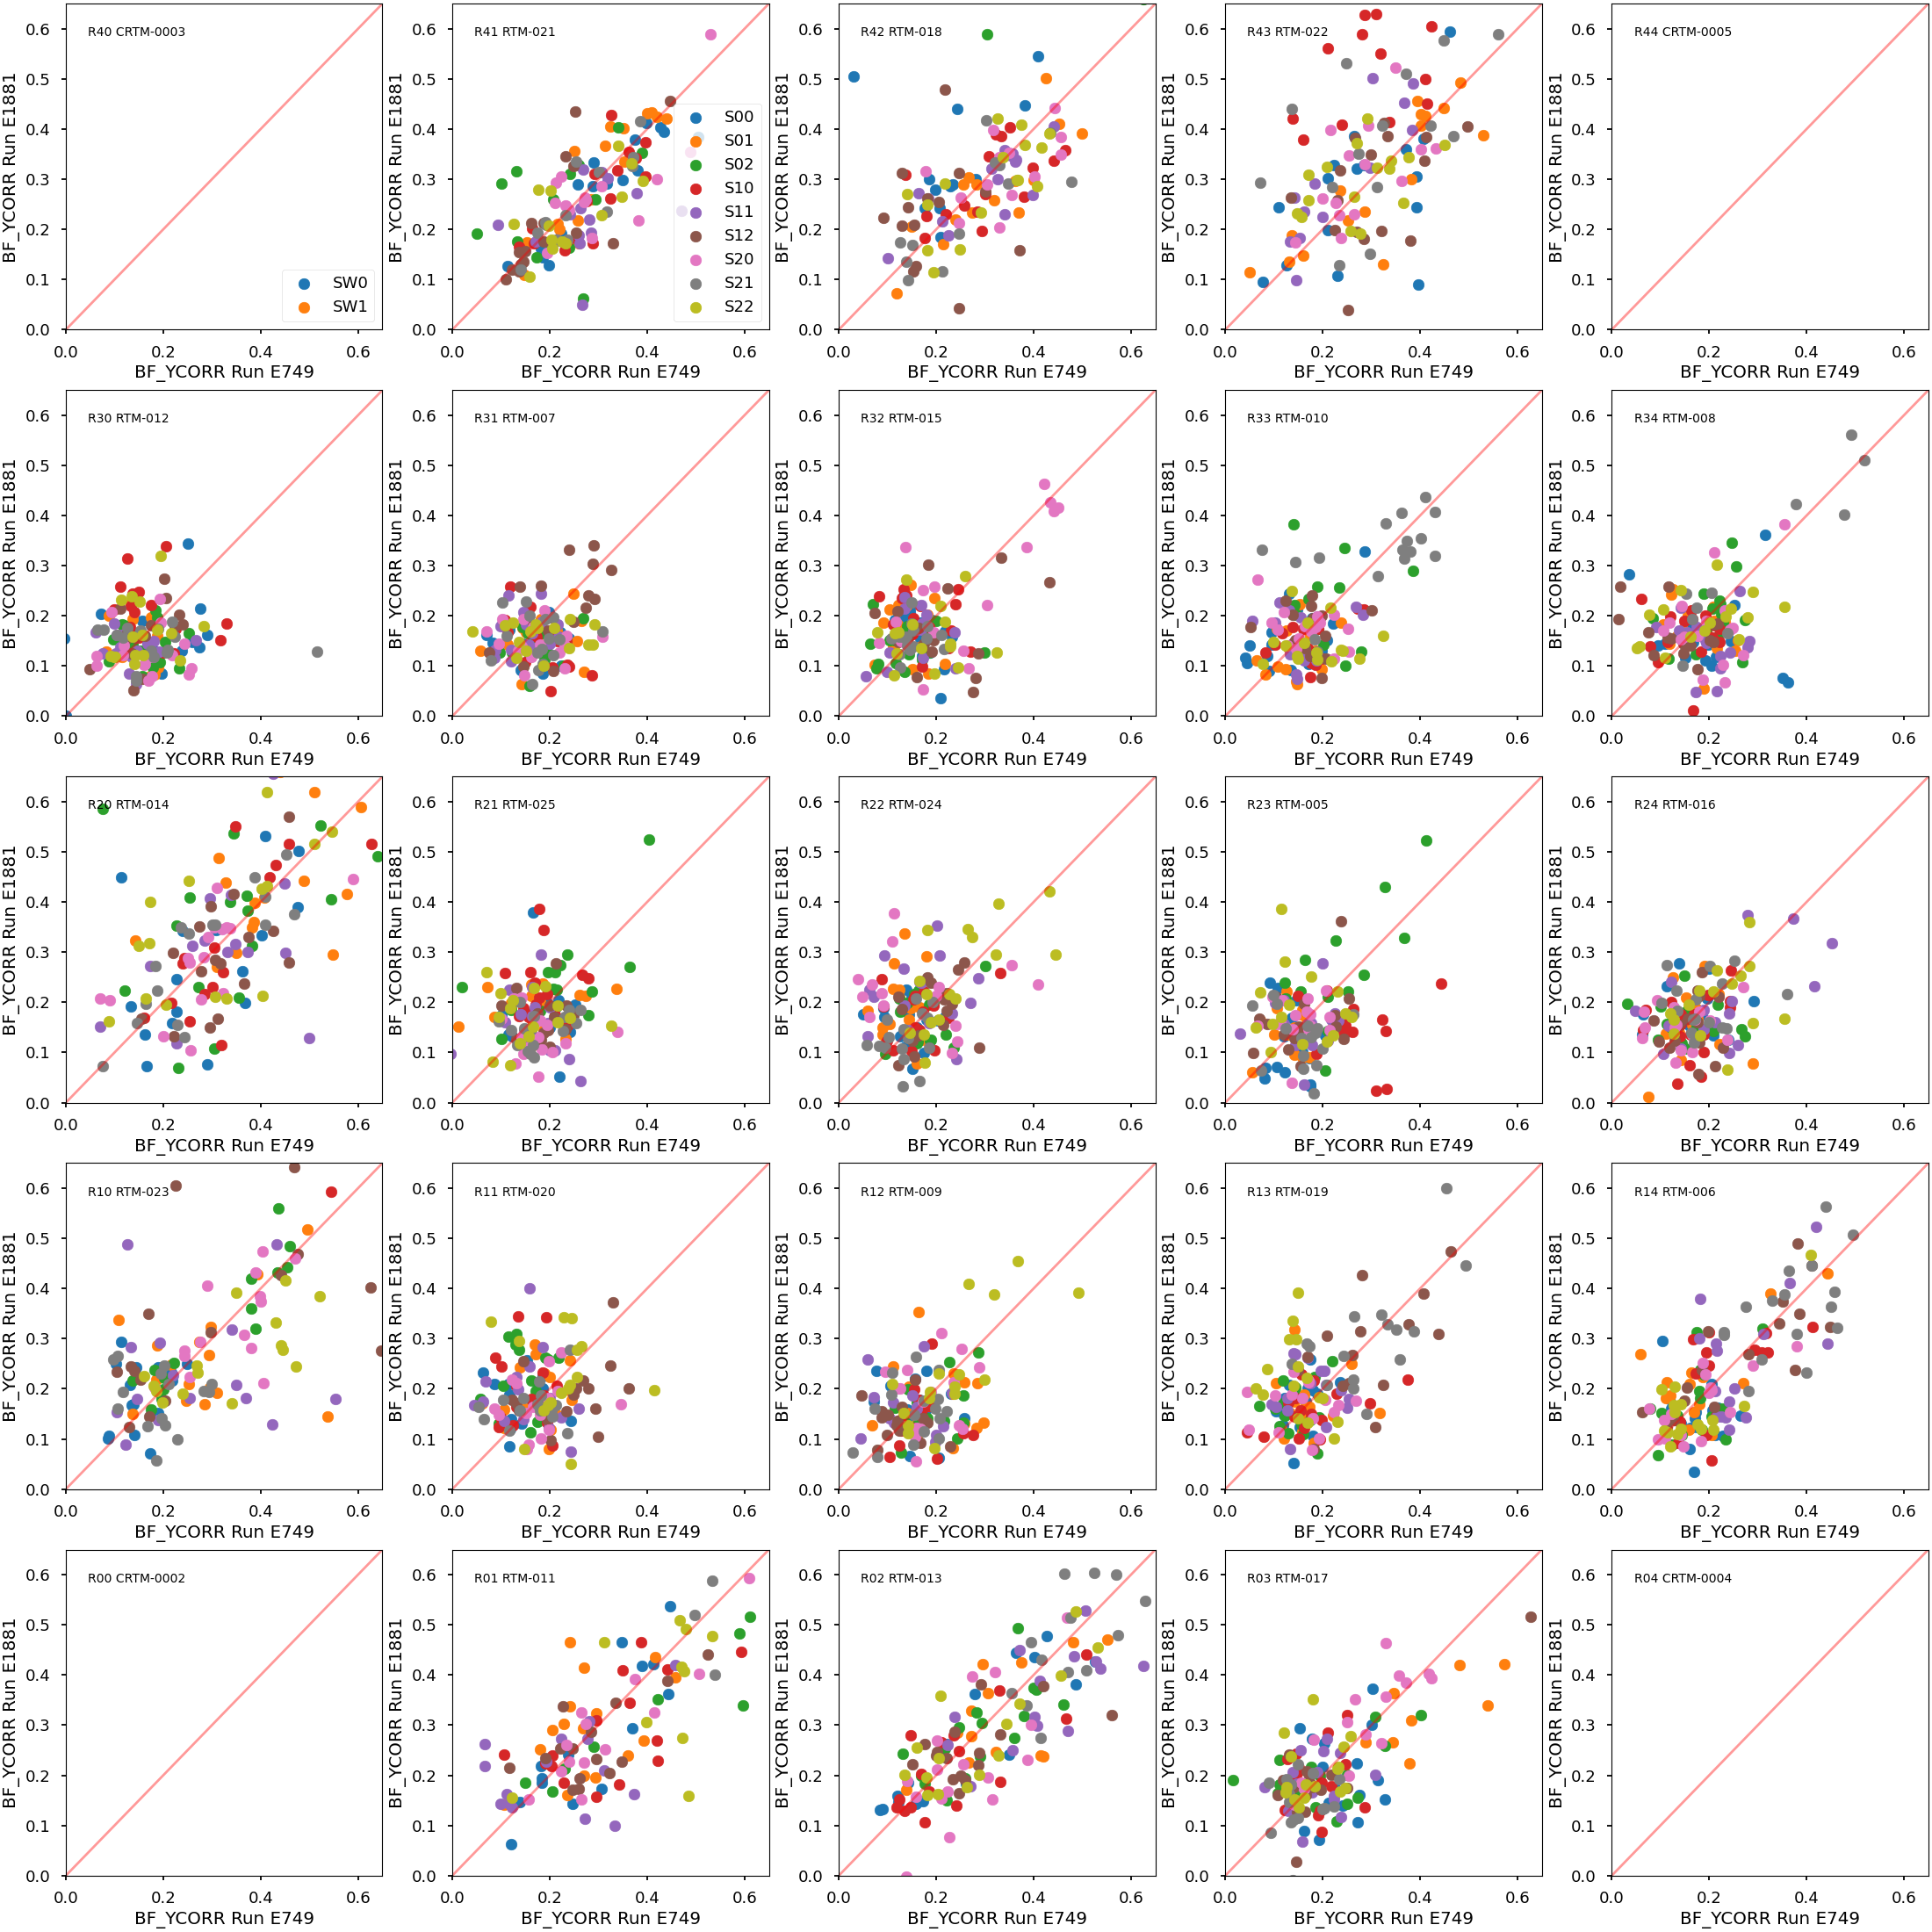
\includegraphics[width=0.7\linewidth]{figures/finalCharacterization/E749_E1881_BF_YCORR.png}
    \caption{Comparison of per-amplifier measurements of the brighter-fatter y-correlation for initial and final Run 7 conditions. For the corner rafts, the correlations are outside of the ranges shown here.}
    \label{fig:finalChar-BFYCorr-5x5}
\end{figure}


\clearpage
\paragraph{Row-means variance}\label{final-row-means-var}

The row means variance is extracted from the PTC runs, and the correlation between the initial and final operating conditions of Run 7 is very tight. The agreement is close for ITL sensors and for e2v sensors row-means variance decreases by \textasciitilde1.8\% in the final operating conditions (Fig.~\ref{fig:finalChar-RowMeanVarSlope-5x5}). Several sensors show a significant change in their final Run 7 row means variance, especially on R42 and R43 (see Fig.~\ref{fig:finalChar-RowMeanVarSlope-5x5}). These sensors record erroneous measurements for other PTC metrics, and warrants further study before making a determination about overall sensor performance.

\begin{figure}[ht]
    \centering
    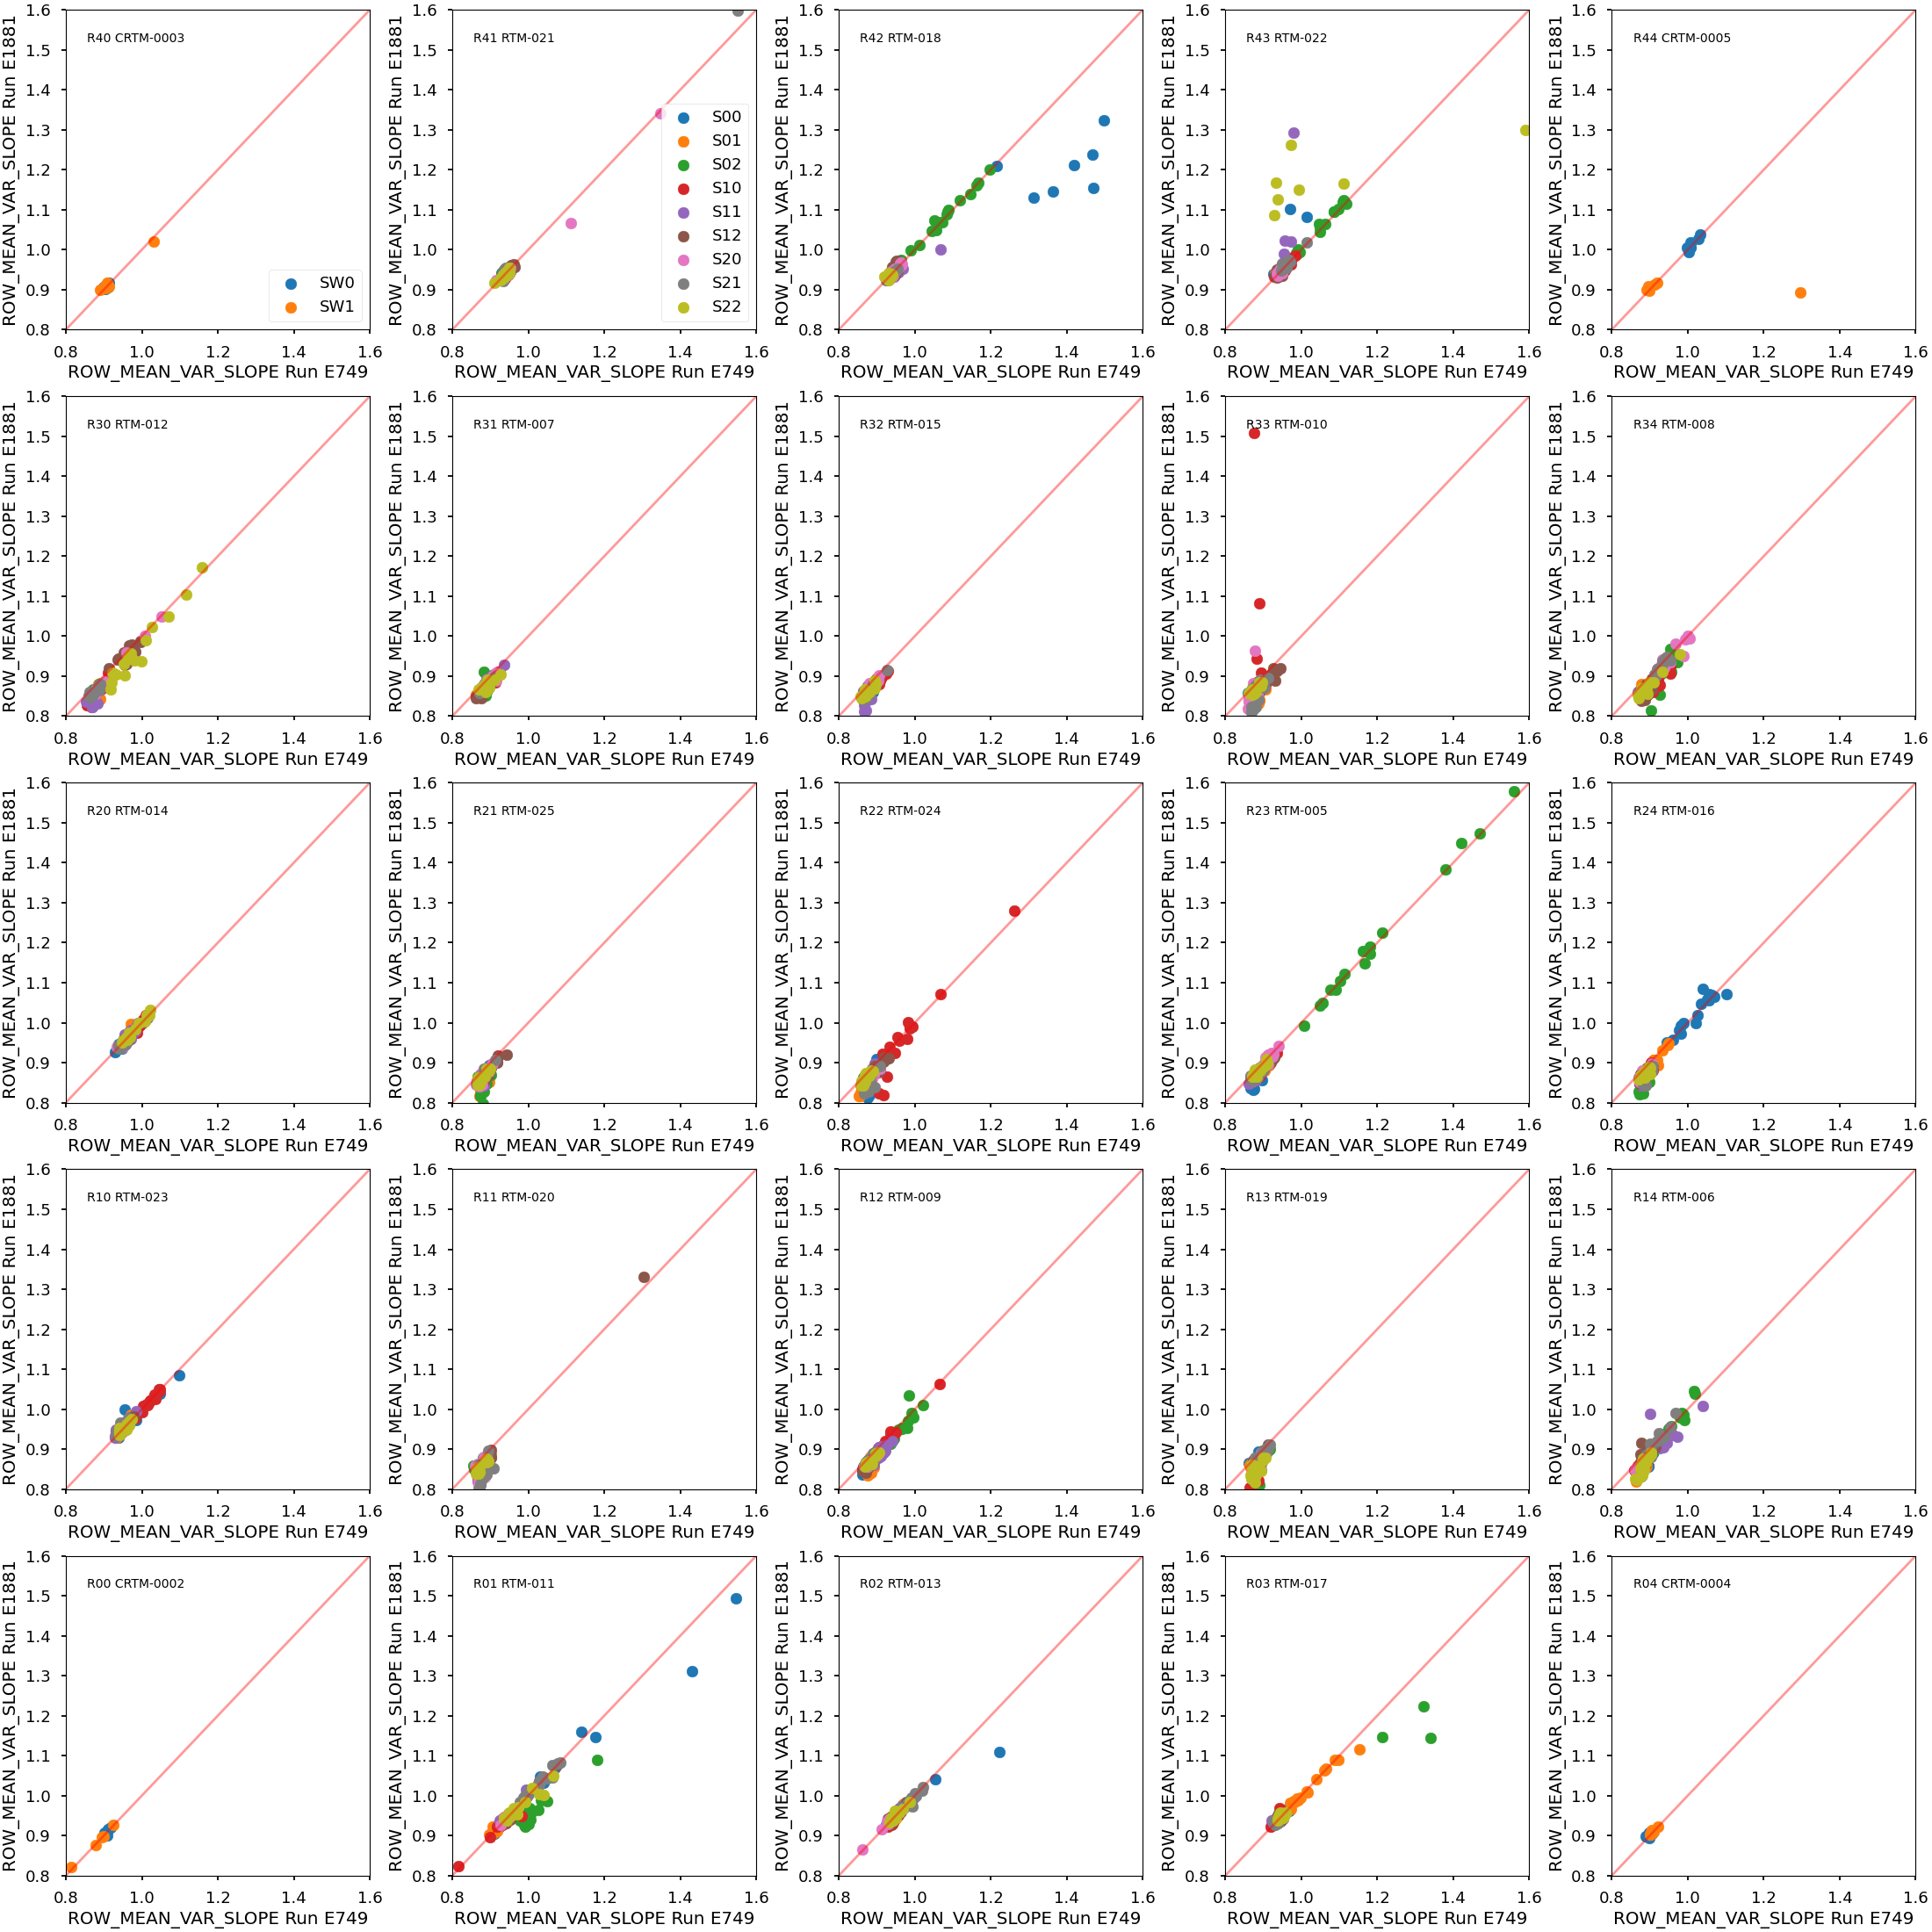
\includegraphics[width=0.7\linewidth]{figures/finalCharacterization/E749_E1881_ROW_MEAN_VAR_SLOPE.png}
    \caption{Comparison of per-amplifier measurements of the row-means variance slope  for initial and final Run 7 conditions.}
    \label{fig:finalChar-RowMeanVarSlope-5x5}
\end{figure}

\clearpage
\paragraph{Divisadero Tearing}\label{final-divisadero-tearing}

Divisadero tearing measurements were extracted from the B protocol runs, and the results are significantly different for e2v sensors in the final operating condition (Fig.~\ref{fig:finalChar-Divisadero-5x5}). The change in divisadero strength is driven by whether idle flush is enabled.  Idle flush is described in detail in Section~\ref{section:disablingIDLEFLUSH}. The e2v sensors show a 61\% decrease in the original divisadero signal under the final operating conditions. ITL sensors show virtually no change (a 0.2\% increase) in the original divisadero signal under the final operating conditions.

\begin{figure}[ht]
    \centering
    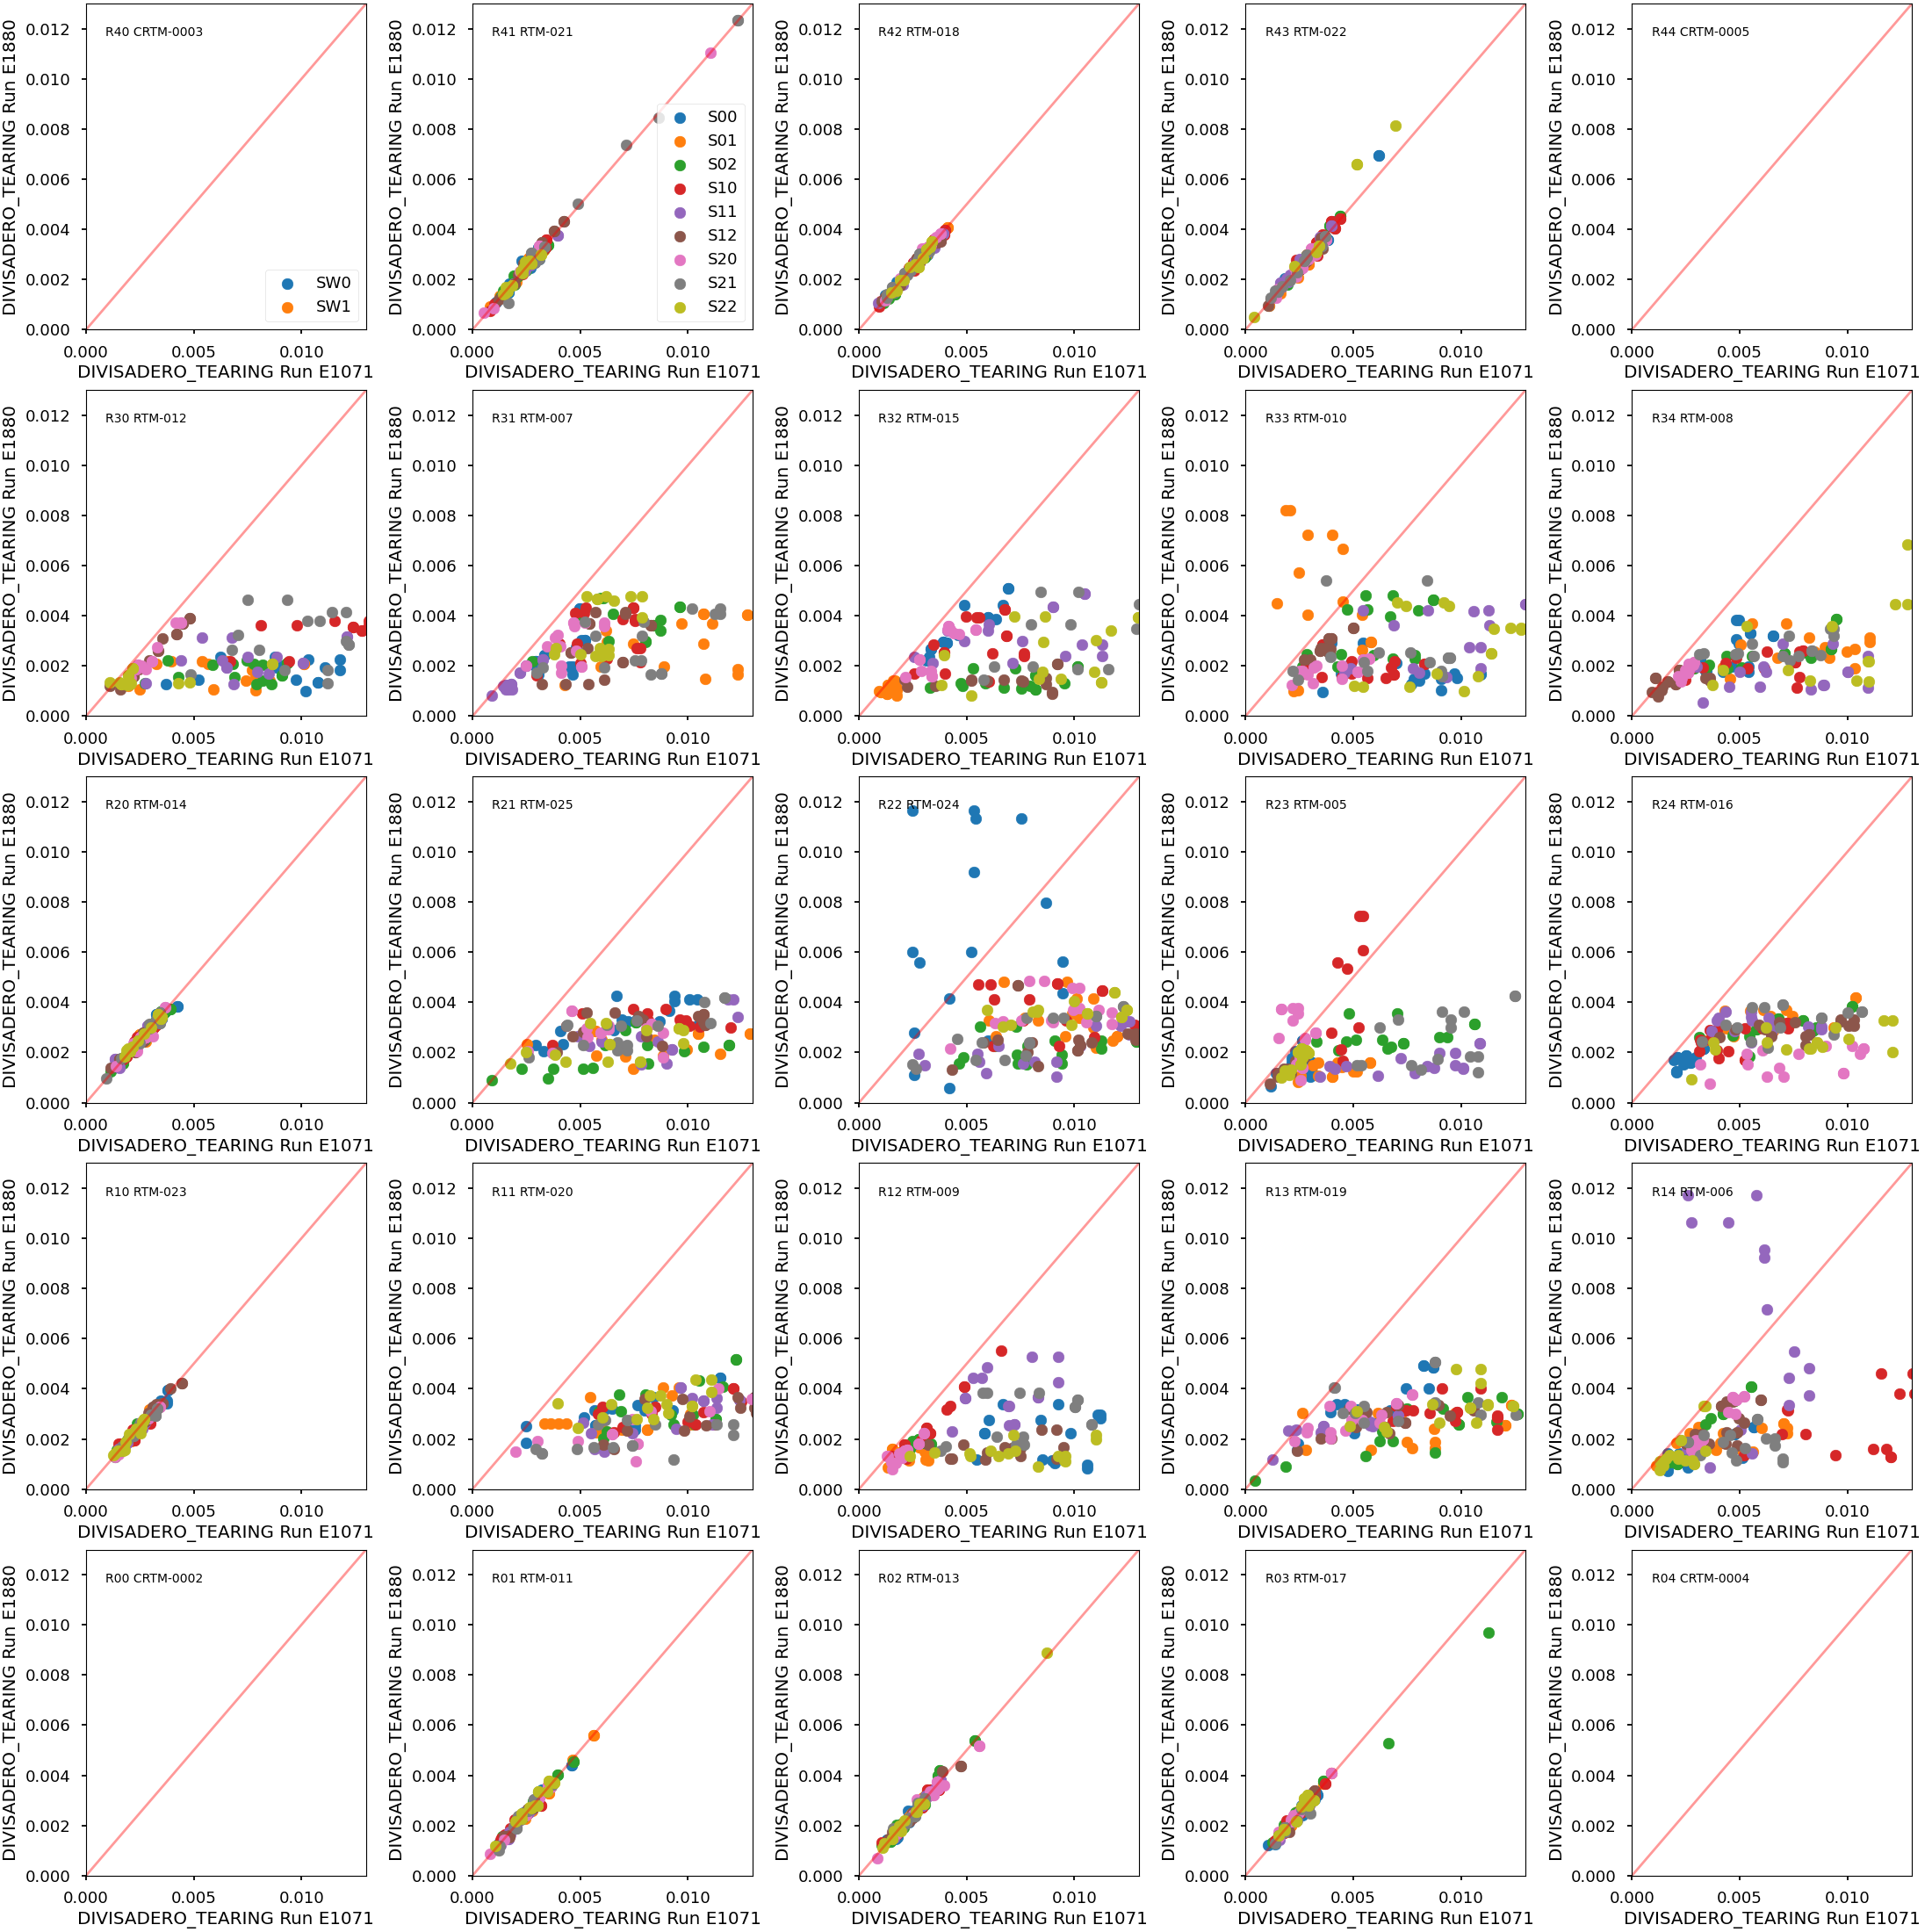
\includegraphics[width=0.7\linewidth]{figures/finalCharacterization/E1071_E1880_DIVISADERO_TEARING.png}
    \caption{Comparison of per-amplifier measurements of divisadero tearing for initial and final Run 7 conditions.}
    \label{fig:finalChar-Divisadero-5x5}
\end{figure}


\clearpage
\paragraph{Dark defects}\label{final-dark-defects}

Dark defects in the LSSTCam sensors were identified using the B protocol runs.  The measurement is contaminated by the picture frame effect regardless of operating conditions (see Sec.~\ref{dark-defects} for additional discussion). When applying a 9 pixel wide mask to the edges of each sensor, the picture frame signal is removed, leaving true dark defects as identified by the analysis pipeline.

\begin{figure}[ht]
    \centering
    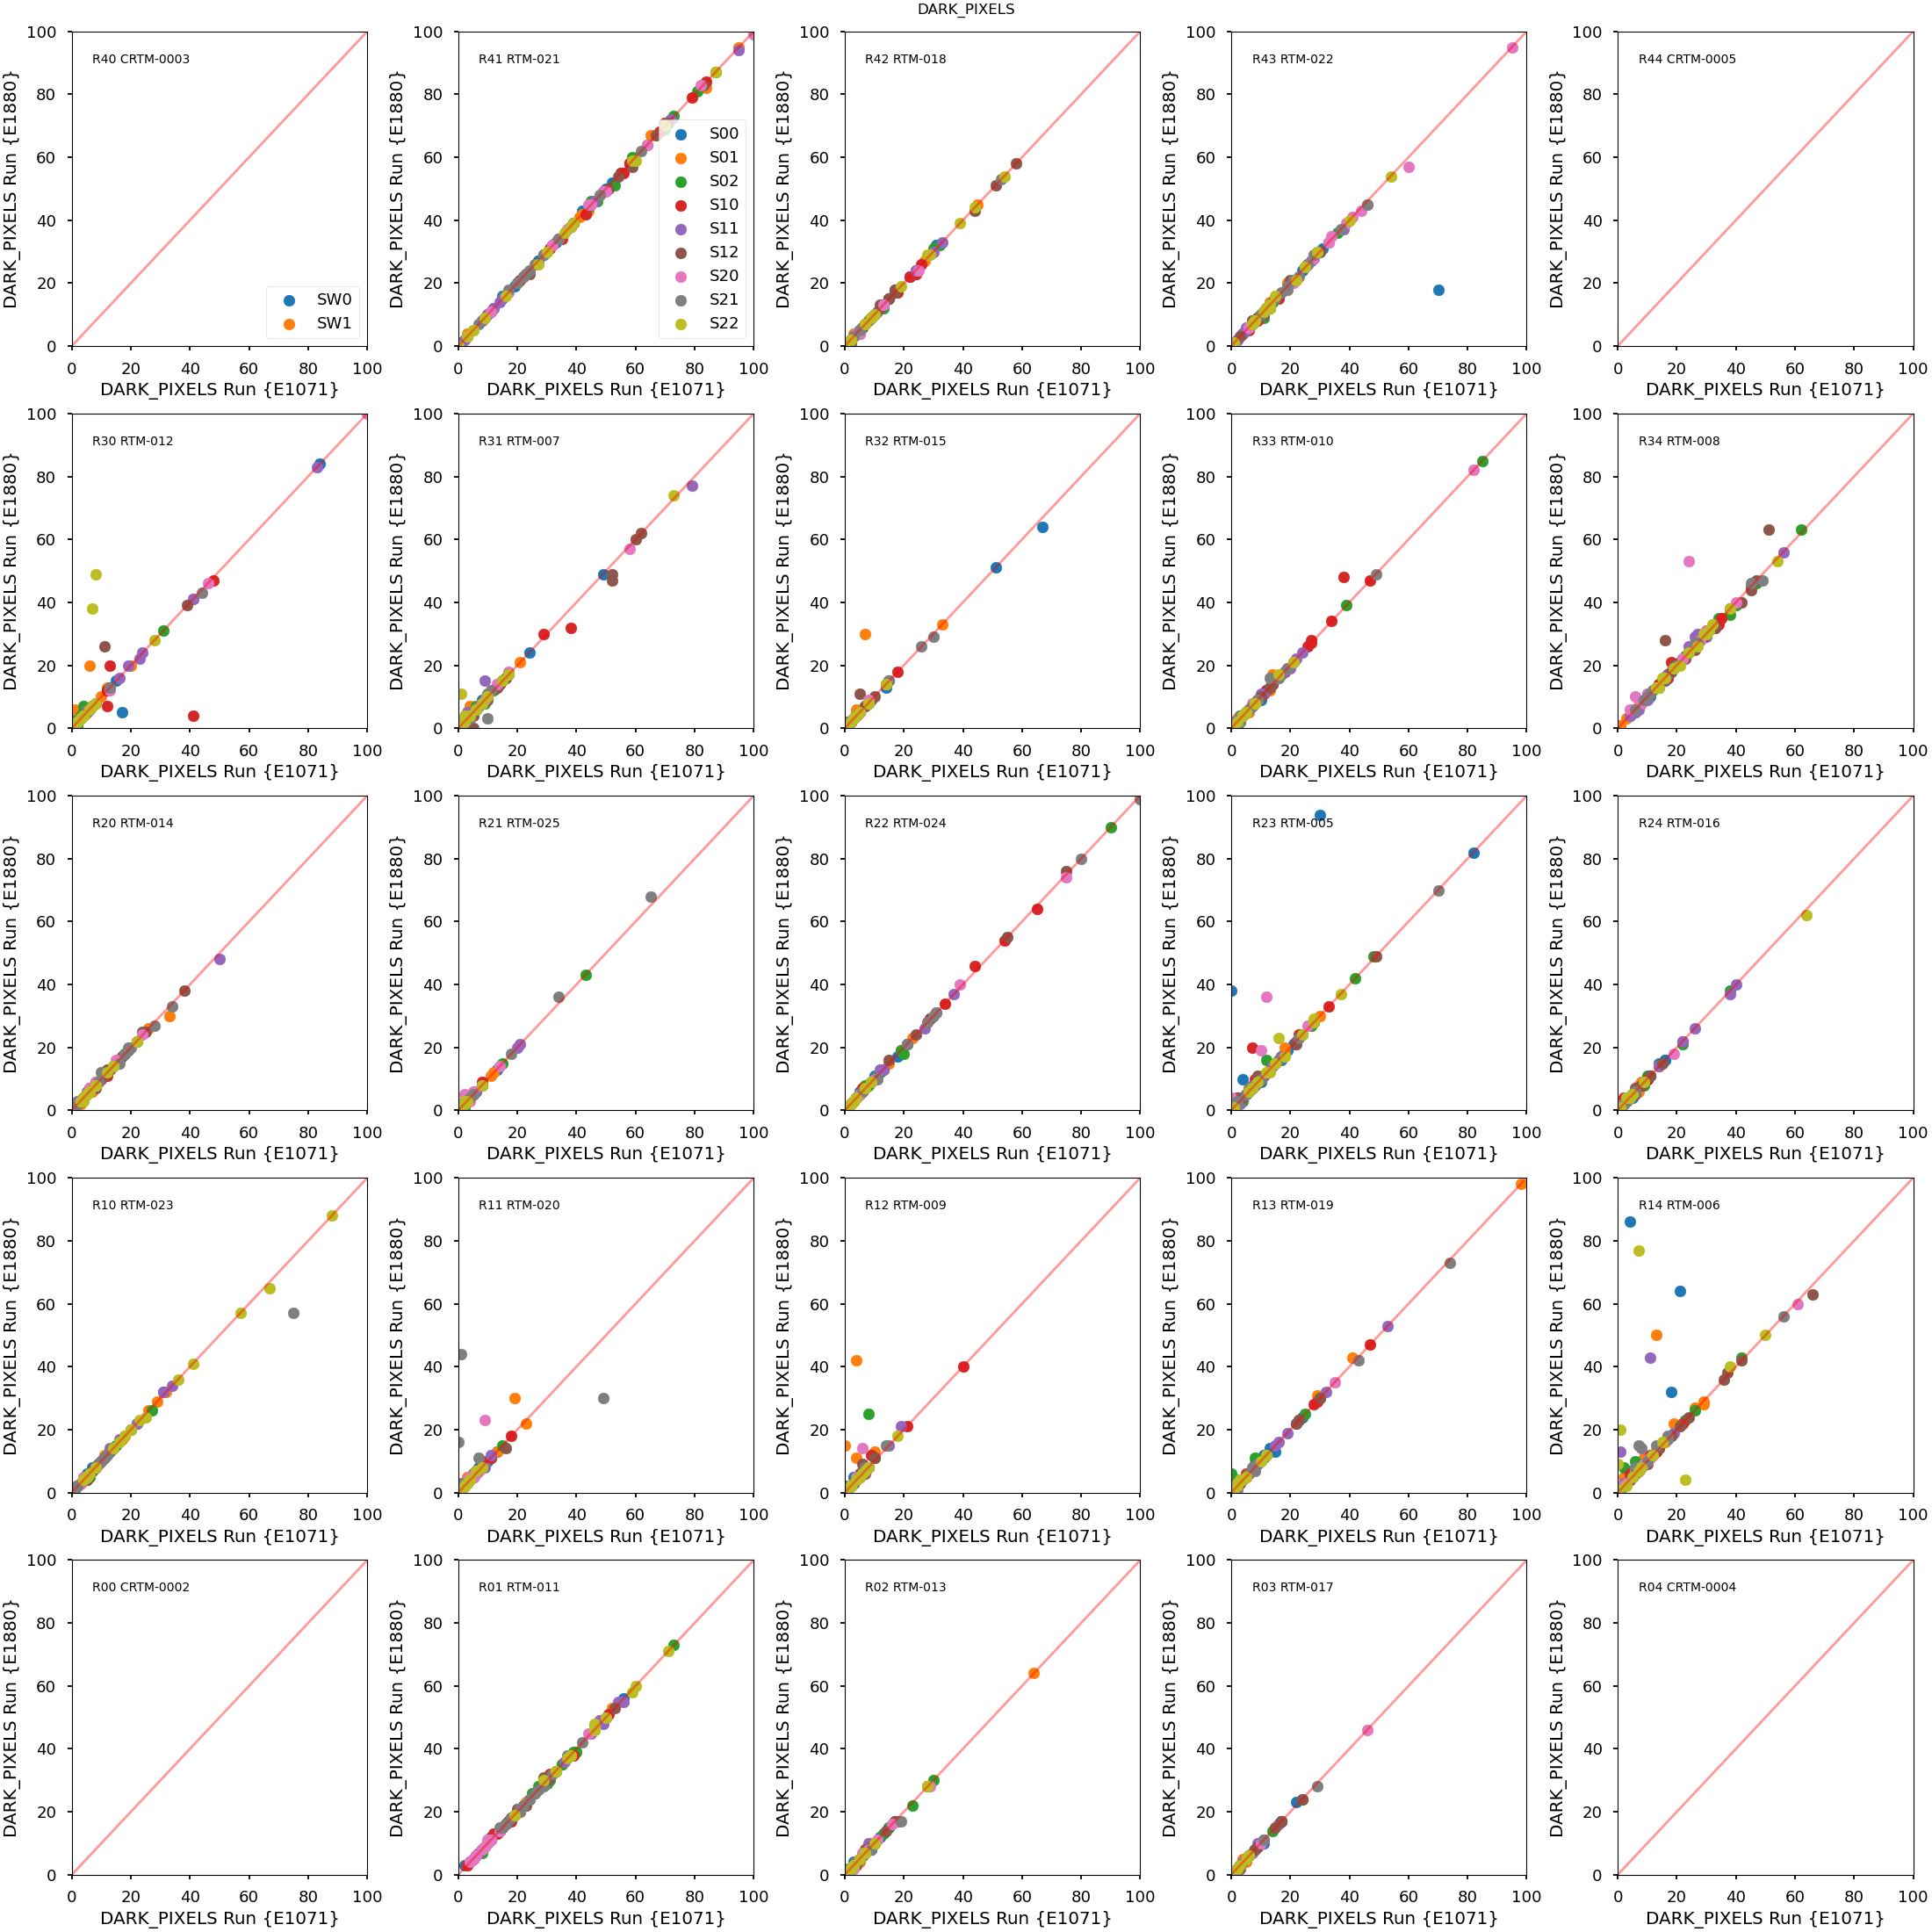
\includegraphics[width=0.7\linewidth]{figures/finalCharacterization/E1880_E1071_DARK_PIXELS_inset.png}
    \caption{Comparison of per-amplifier measurements of the dark pixel for initial and final Run 7 conditions.}
    \label{fig:finalChar-DarkPix-5x5}
\end{figure}

Dark defects are consistent between initial and final Run 7 runs (Fig.~\ref{fig:finalChar-DarkPix-5x5}). Dark defects constitute a very small fraction of the pixels in the focal plane, with an average contribution of 3 pixels per e2v image segment and 8 pixels per ITL image segment. There is no global change in dark defect counts per segment, with the change of
dark pixel counts per detector centered on zero for both detector types (see Fig.~\ref{fig:finalChar:darkDefectsComparison}).

\begin{figure}[ht]
    \centering
    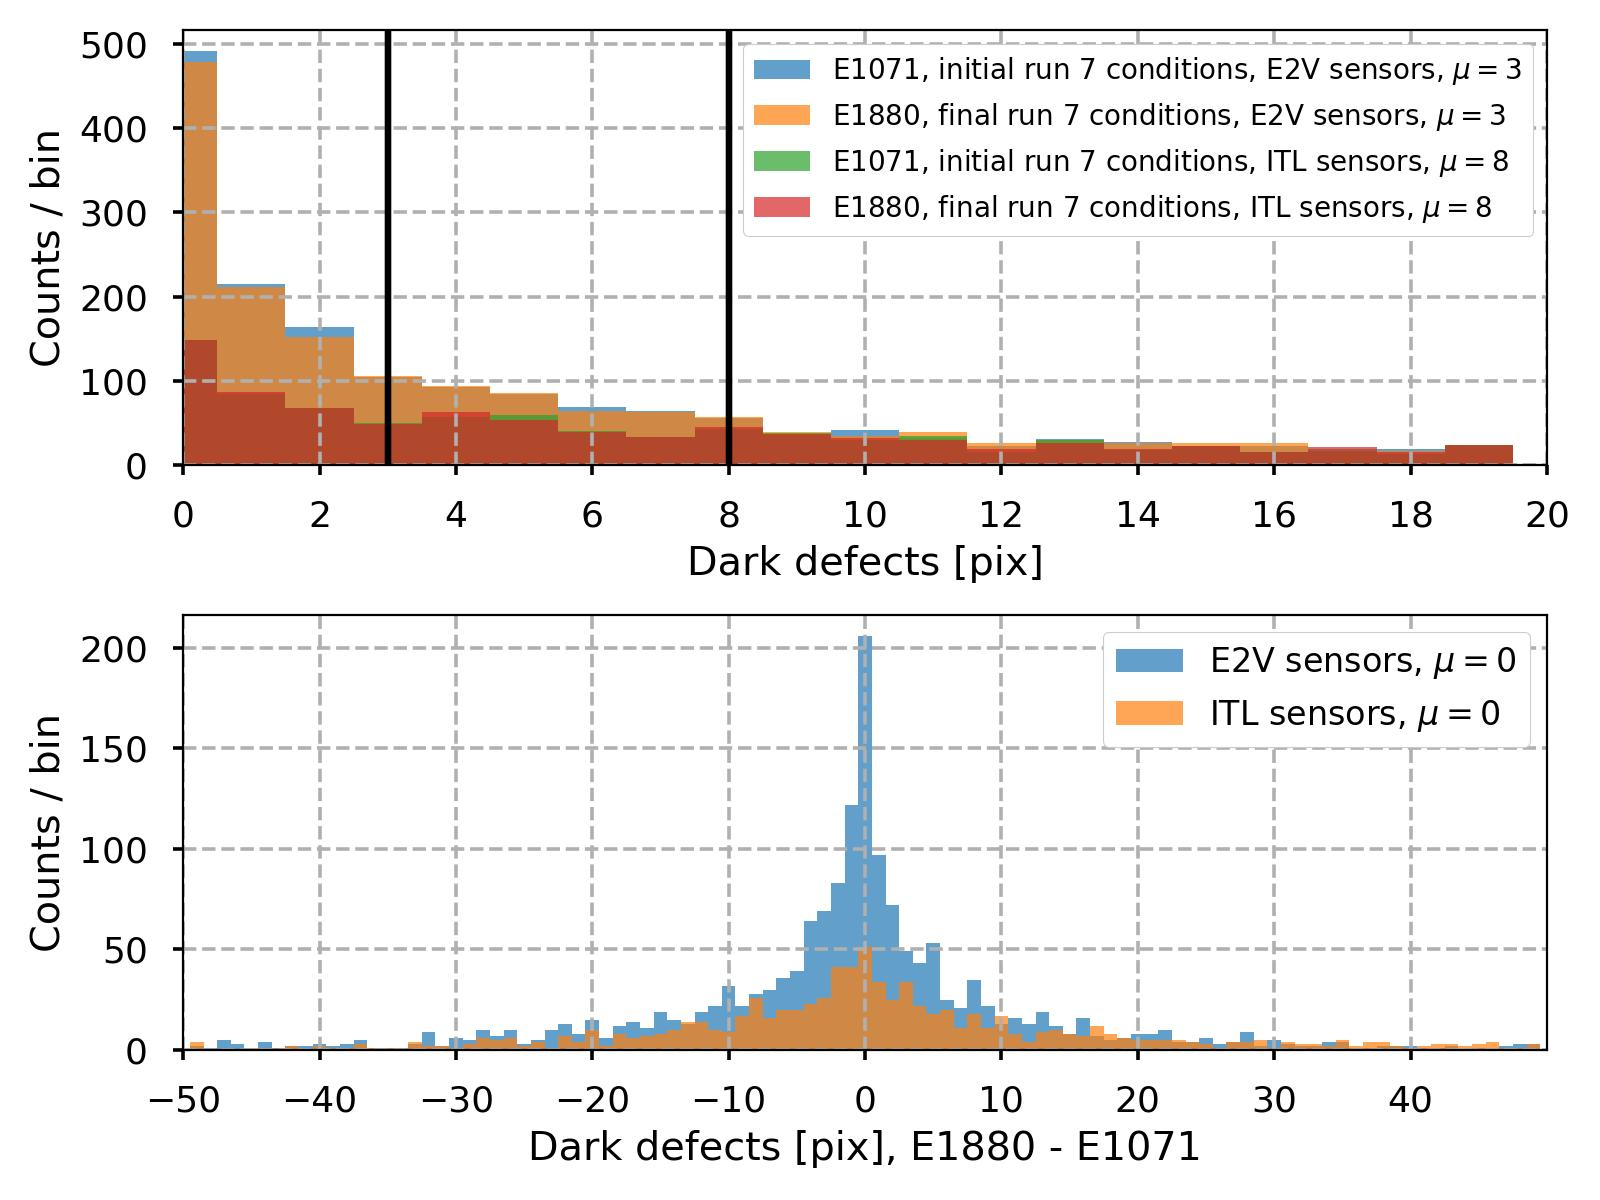
\includegraphics[width=0.9\linewidth]{figures/finalCharacterization/darkDefects_comparison_final.jpg}
    \caption{The per-amplifier distributions of measurements of dark defect pixel counts, with a 9 pixel mask applied to each sensor. Top: A histogram of the dark pixel measurements, with each count representing one amplifier. Histogram groups are separated by sensor type, and also by initial (E1071) and final (E1880) runs. Bottom: The difference in amplifier dark pixel measurements, by detector type. For both types, no significant evolution in the defect counts is evident.}
    \label{fig:finalChar:darkDefectsComparison}
\end{figure}

\clearpage
\subsubsection{Persistence}\label{final-persistence}

The primary optimization goal of Run 7 was to mitigate the persistence effect, described in Section~\ref{persistence-optimization-1}. The major change in the final LSSTCam operating conditions to combat persistence is decreased parallel swing. This change is applied to the e2v sensors only, as they are the sensors that exhibit \geq 1 ADU persistence in 15s exposure intervals with the Run 7 initial operating parameters.

\begin{figure}[ht]
    \centering
    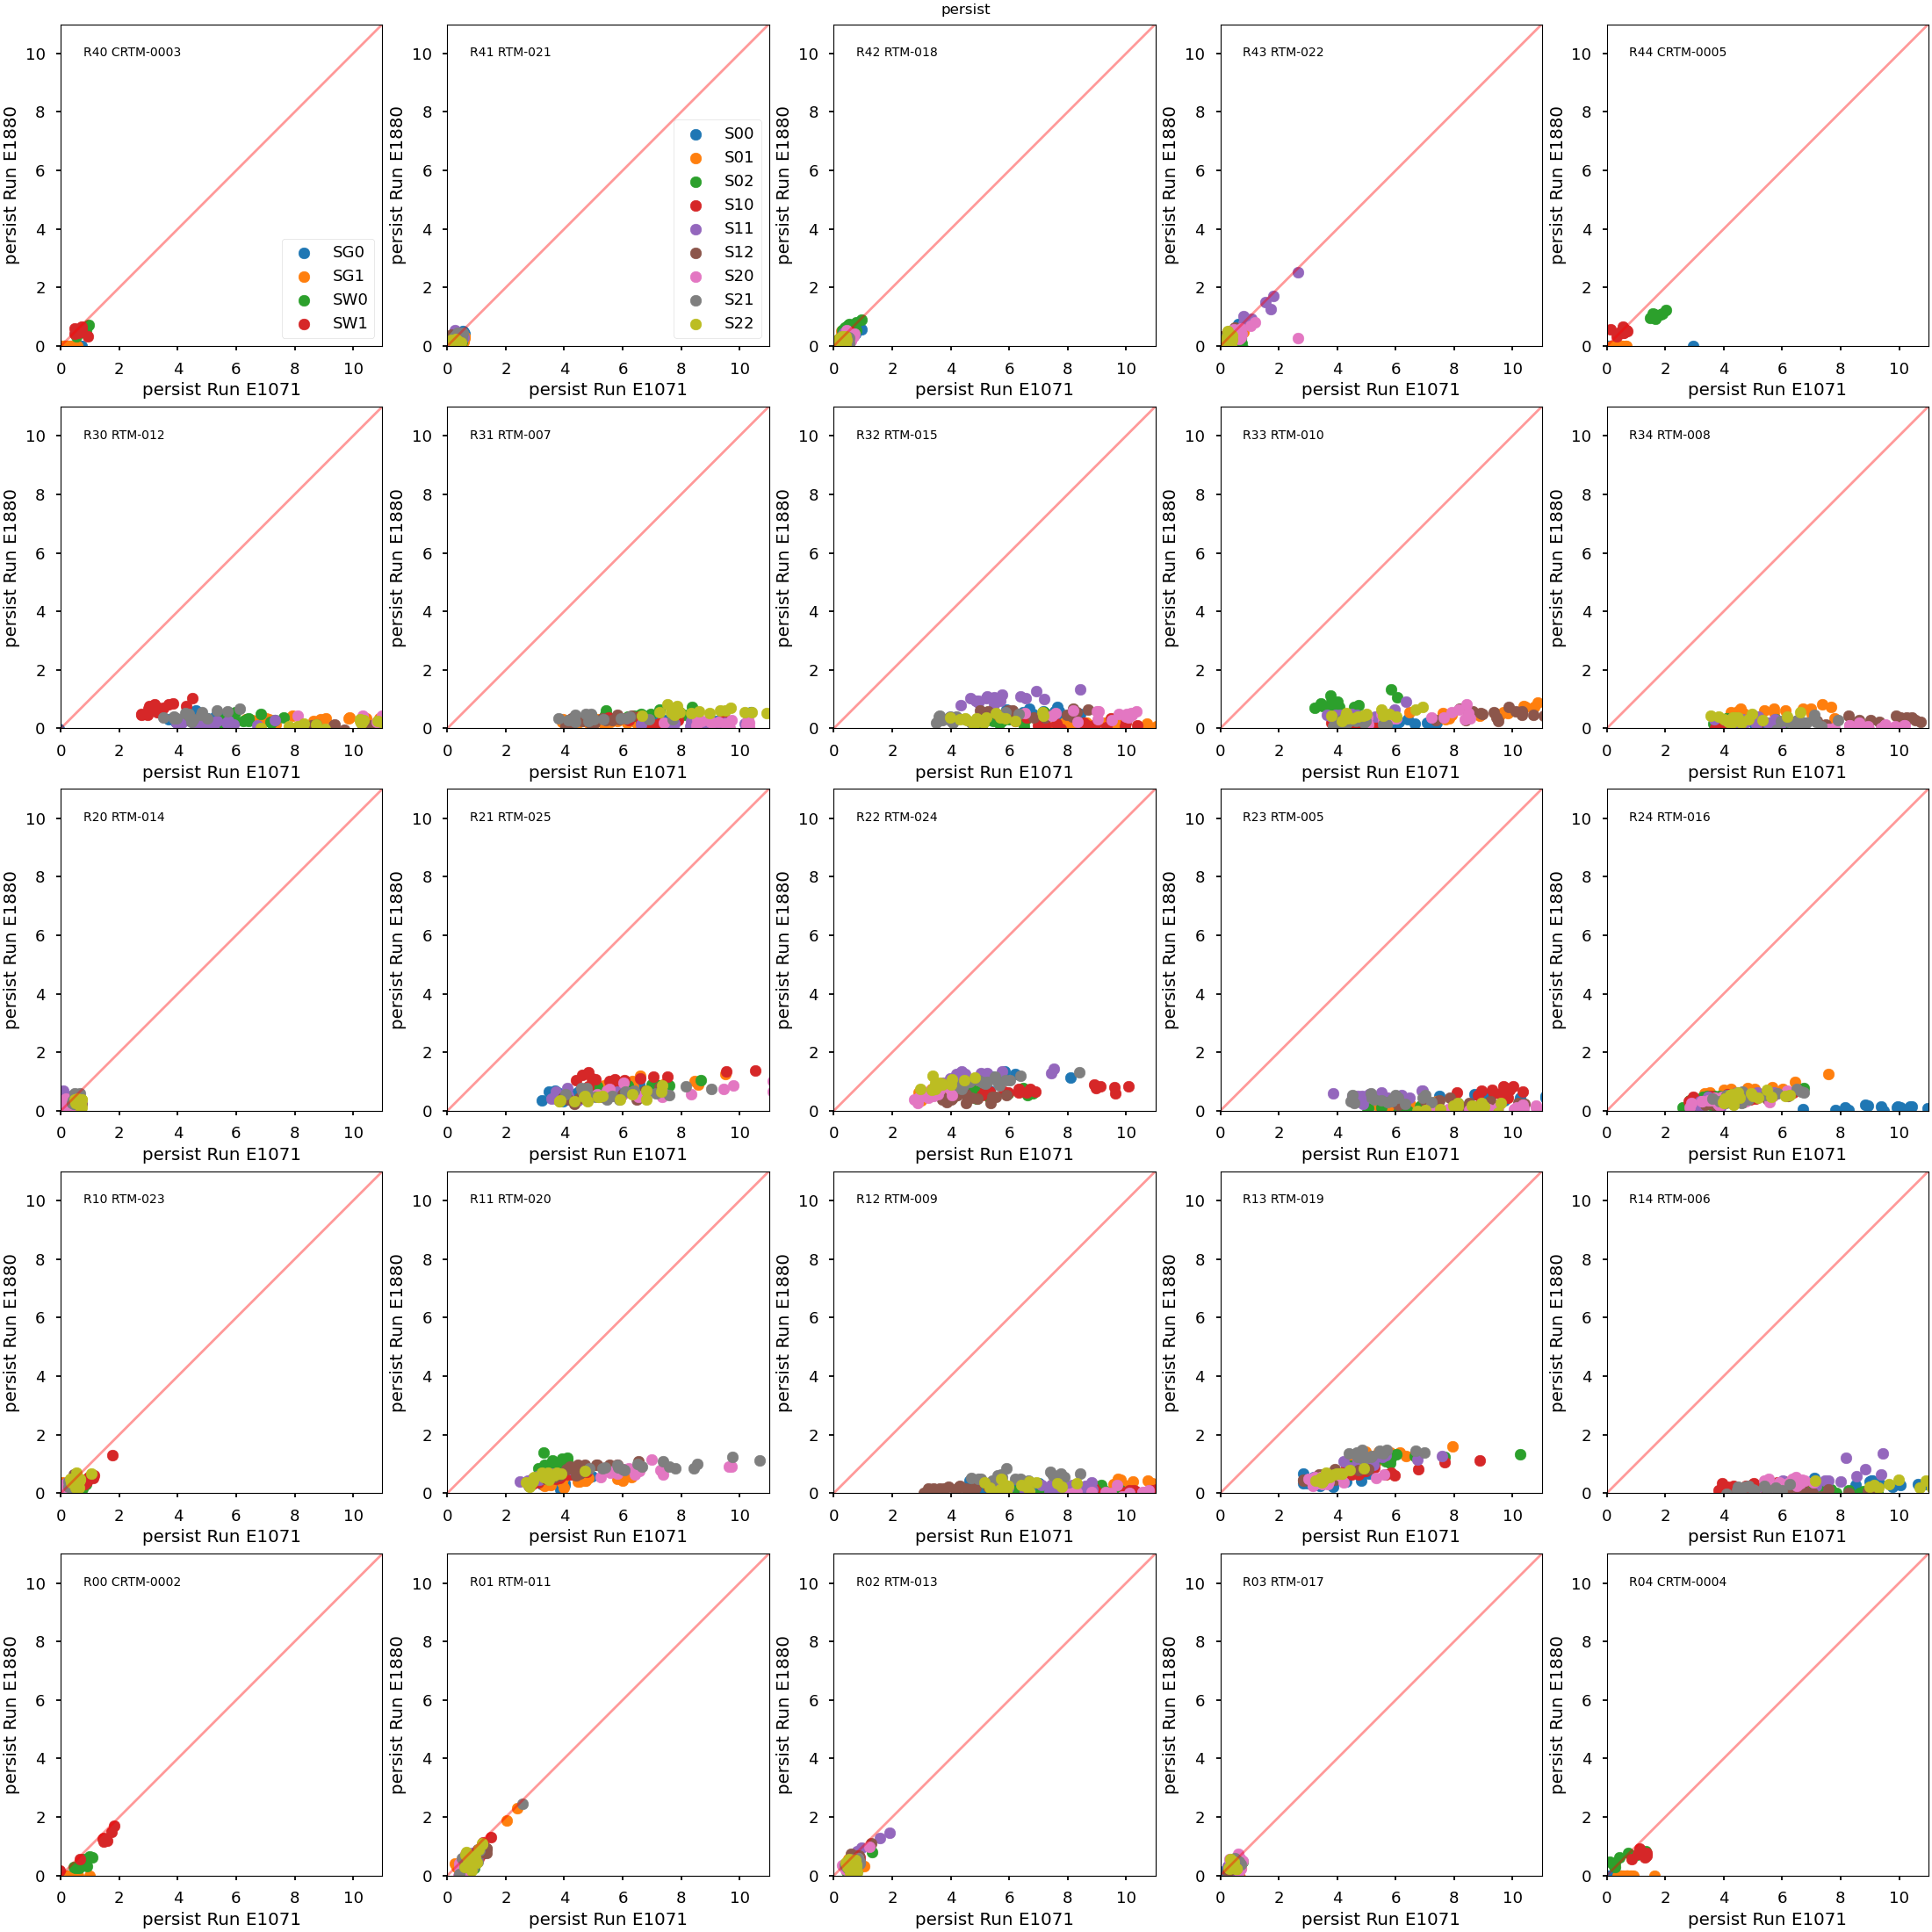
\includegraphics[width=0.7\linewidth]{figures/finalCharacterization/E1071_E1880_persist_inset.png}
    \caption{Comparison of per-amplifier measurements of persistence for initial and final Run 7 conditions.}
    \label{fig:finalChar-Persist-5x5}
\end{figure}

The per-amplifier measurements of persistence using the metric described in Section~\ref{sec:initPersistenceChar} show a significant decrease in persistence signal in e2v sensors due to the lower parallel swing (Fig.~\ref{fig:finalChar-Persist-5x5}), from 5.7\,ADU \rightarrow 0.4\,ADU on average when measured using the red LED (corresponding to the LSST r band filter).

\begin{figure}[ht]
    \centering
    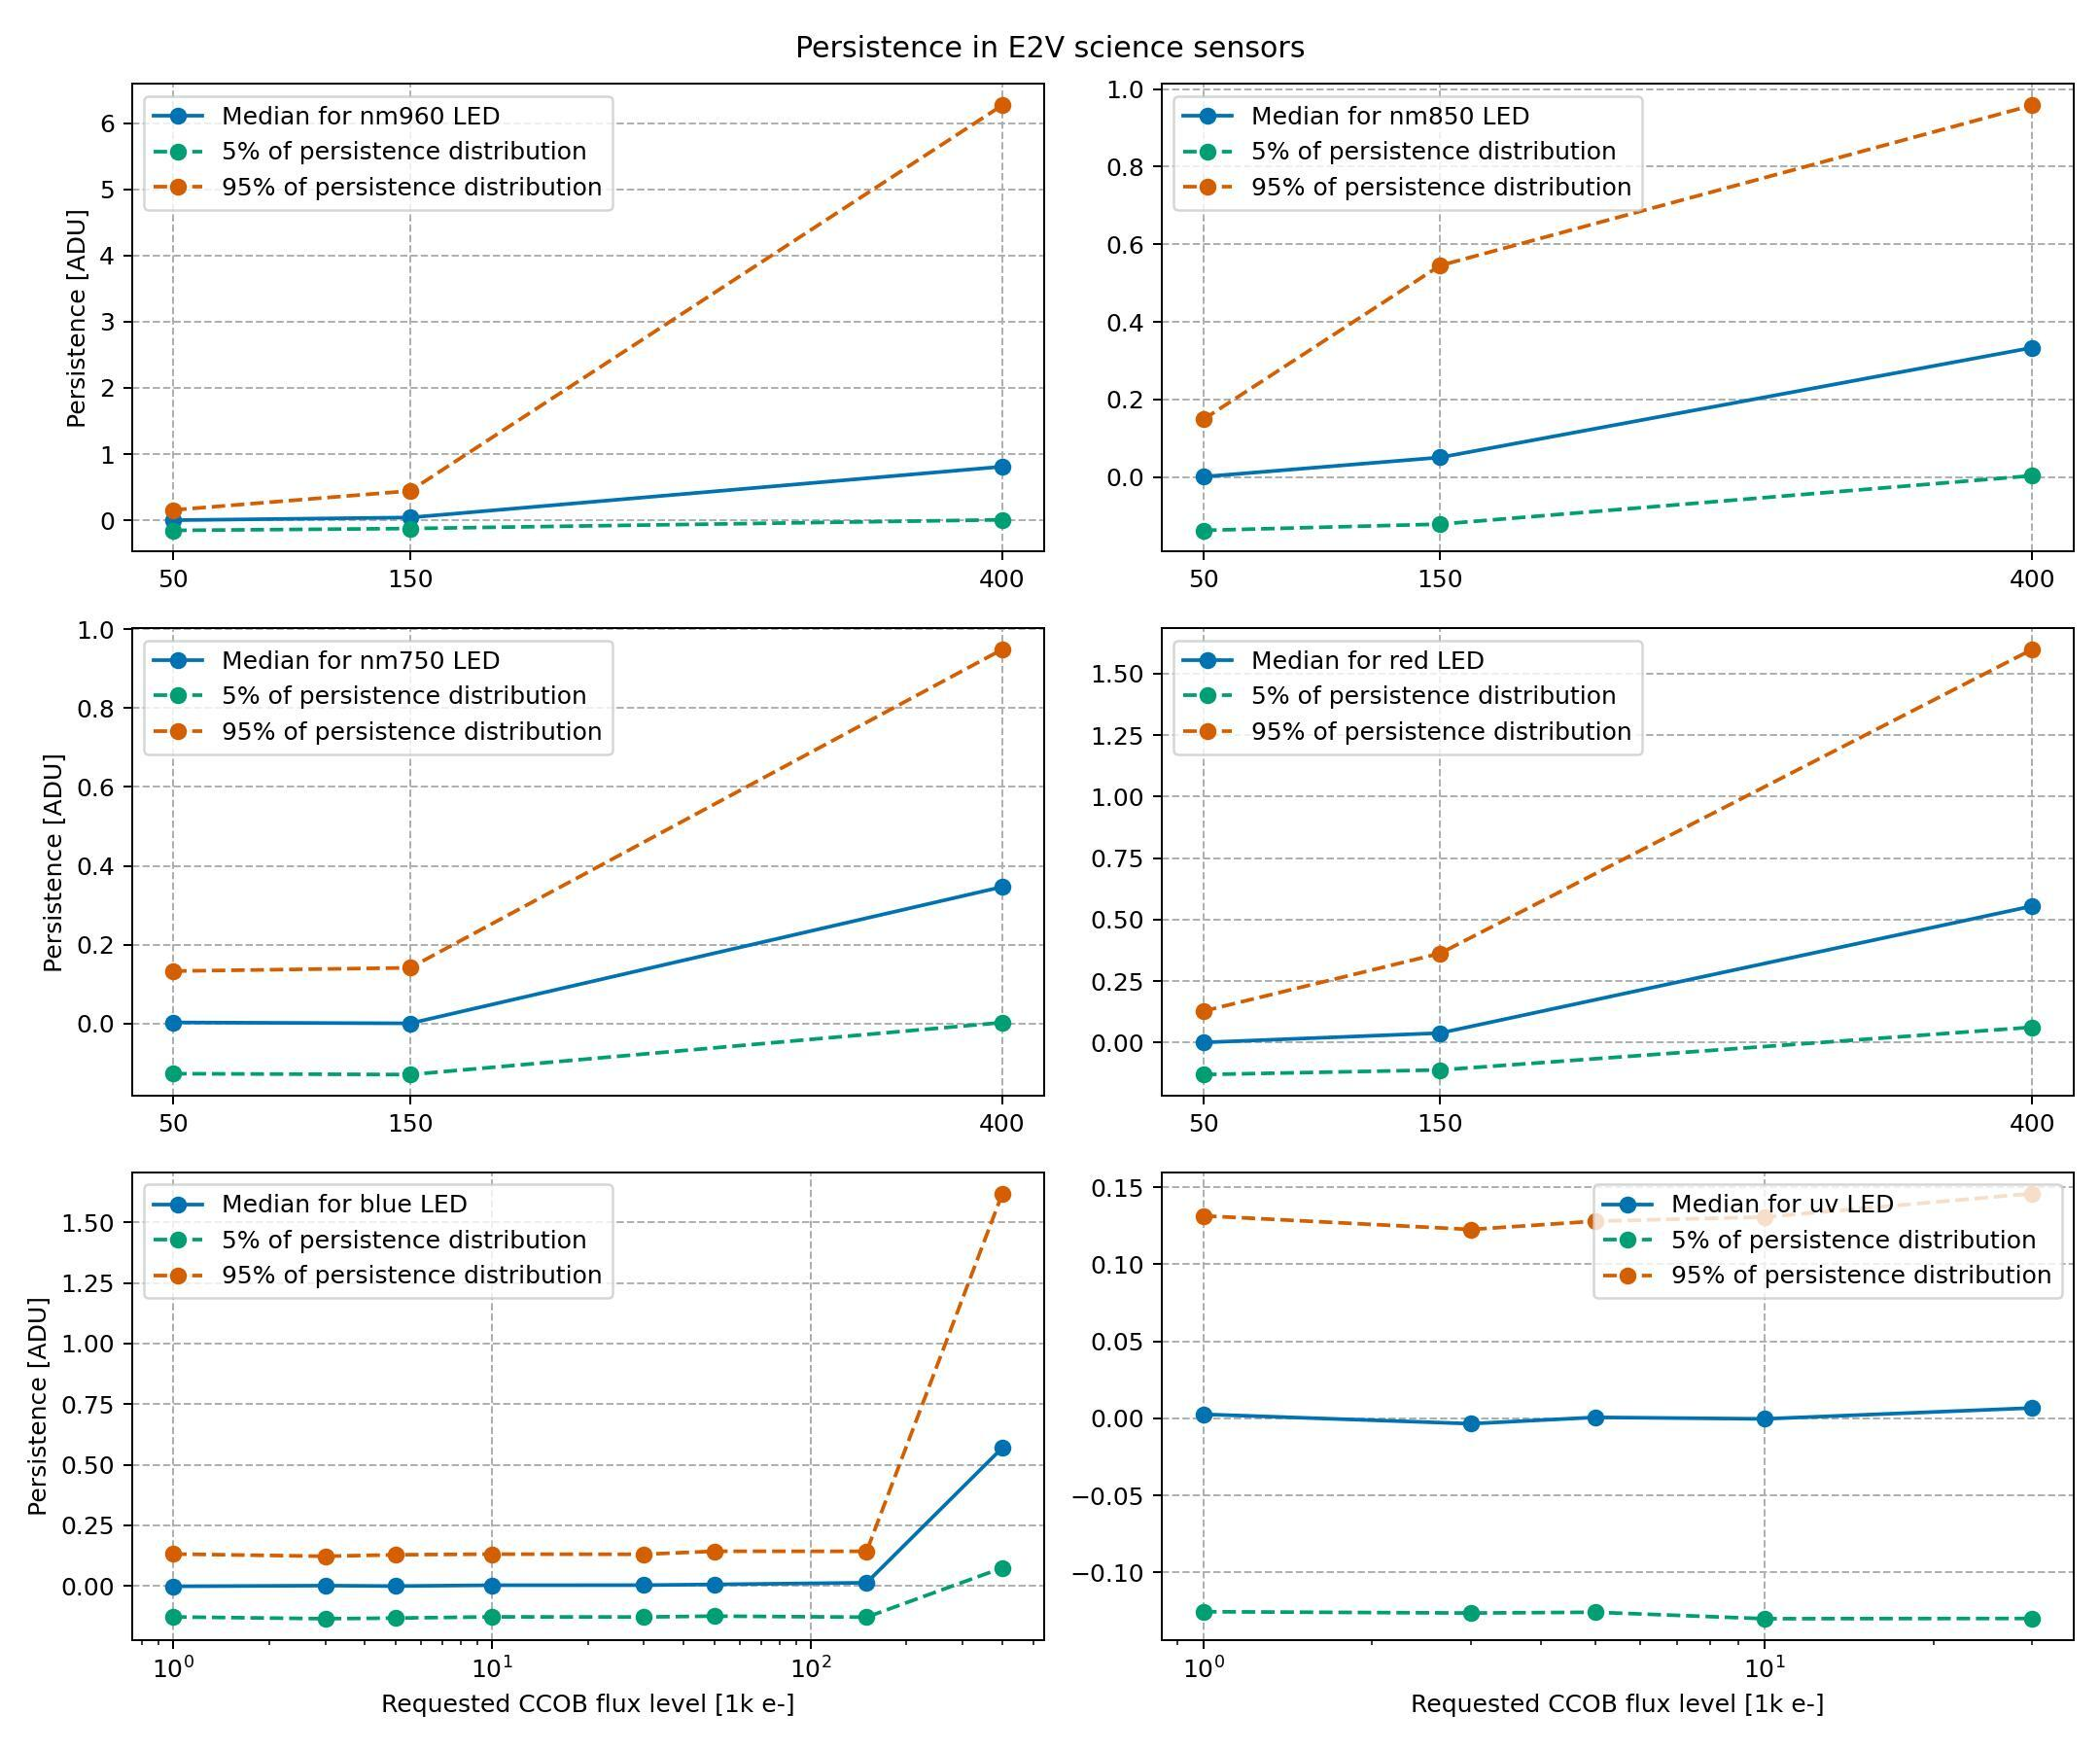
\includegraphics[width=0.7\linewidth]{figures/PersistenceE2V.jpg}
    \caption{Demonstration of persistence mitigation in e2v sensors in the final operating condition. Persistence runs are acquired at different flat illuminations and LEDs. For e2v sensors, $\geq95\%$ of segments show $\leq1$ ADU persistence for all exposures below linearity. The measurements of persistence below 0 ADU are due to offsets in the bias subtraction when making the frame calibration and not a feature of the persistence measurement.}
    \label{fig:finalChar-persistenceAllLEDs}
\end{figure}

B protocol runs acquire persistence datasets using the red LED, which is flashed to provide equivalent of 400k e- per pixel, i.e., saturation only (a description of B protocol persistence acquisitions is provided in Sec.~\ref{background}). Additional persistence datasets were acquired using other LEDs and other exposure levels with the CCOB wide beam projector. This was to verify that persistence was mitigated for the complete LSST photometric range. The runs used for this analysis are listed in Table~\ref{table:runs_persistence}.

We find that $\geq$95\% of e2v sensors exhibit a persistence signal $\leq$ 0.55 ADU at all flux levels below full-well capacity. The CCOB illumination varied by $\sim$ 10\% across the focal plane, and the maximum PTC turnoff for e2v amplifiers under the final operating conditions was 123k\,e- (see Fig.~\ref{fig:finalChar-fullWell}), within the flux levels probed in Figure~\ref{fig:finalChar-persistenceAllLEDs}.

\subsubsection{Differences between Run 7 initial and Run 7 final measurements}\label{final-differences-from-previous-runs}

Comparing the initial and final Run 7 measurements, four metrics are impacted by the optimization efforts described in Section~\ref{sec:camera-optimization}.
\begin{itemize}
  \item \textbf{Persistence:} We minimized persistence in e2v sensors, the main optimization target of Run 7, decreasing it from 5.66 ADU to 0.40 ADU on average with the red LED (LSST-r band), and maintaining sub-ADU levels across the entire LSST bandpass. Due to no change in ITL voltages and lack of an initial persistence feature, ITL sensors do not show a significant change in persistence, and remain at a sub-ADU level (0.48 ADU \rightarrow 0.32 ADU).
  \item \textbf{Full well capacity:} As a direct consequence of lower parallel swing in e2v sensors, the full-well capacity of e2v sensors decreased significantly with the final operating parameters. For linearity turnoff, e2v sensors decrease from 167,796 e- \rightarrow 136,302 e-. PTC turnoff measurements decrease from 132,963 e- \rightarrow 102,713 e-. ITL sensors do not show a significant change, and remain consistent between initial and final runs.
  \item \textbf{Brighter-fatter strength (PTC $a_{00}$):} The strength of the brighter-fatter effect is also significantly impacted by the change in parallel swing for e2v sensors. The $a_{00}$ parameter increases from $3.08\times10^{-6} \rightarrow 3.49\times10^{-6}$ for e2v sensors, a 13\% increase. ITL sensors are not significantly impacted.% Consequence of changed dP
  \item \textbf{Divisadero:} The strength of divisadero tearing is impacted by idle flush. For e2v sensors, we measure a reduction in maximum divisadero signal from 0.62\% \rightarrow 0.25\%, a 60\% reduction in signal. ITL sensors did not exhibit a strong divisadero signal under the initial conditions, and therefore did not measure a reduction in maximum divisadero signal (0.273\% \rightarrow 0.274\%). The initial strength of divisadero tearing in ITL sensors is taken as a reference size, and is therefore not minimized by the change in idle flush.
\end{itemize}

\begin{table}[ht]
\centering
\resizebox{\textwidth}{!}{ % Resize the table to the page width
\begin{tabular}{|l|l|ll|ll|}
\hline
\multirow{2}{*}{Parameter [unit]} & \multirow{2}{*}{Specification} & \multicolumn{2}{l|}{e2v}                   & \multicolumn{2}{l|}{ITL}                    \\ \cline{3-6}
                                  &                                & \multicolumn{1}{l|}{R7 initial} & R7 final & \multicolumn{1}{l|}{R7 initial} & R7 final \\ \hline
Serial CTI {[}\%{]}               &           $5\times10^{-4}$                     & \multicolumn{1}{l|}{1.1$\times10^{-5}$}              &      7.3$\times10^{-6}$       & \multicolumn{1}{l|}{1.7$\times10^{-4}$}              &        1.5$\times10^{-4}$     \\ \hline
Parallel CTI {[}\%{]}             &           $3\times10^{-4}$                     & \multicolumn{1}{l|}{1.1$\times10^{-5}$}              &       1.1$\times10^{-5}$      & \multicolumn{1}{l|}{-4.8$\times10^{-6}$}              &       1.2$\times10^{-6}$      \\ \hline
Dark current {[}e-/pix/s{]}       &             None                   & \multicolumn{1}{l|}{0.025}              &       0.023      & \multicolumn{1}{l|}{0.021}              &       0.021      \\ \hline
Bright defects {[}count{]}        &              None                  & \multicolumn{1}{l|}{0}              &   0          & \multicolumn{1}{l|}{0}              &          0   \\ \hline
Linearity turnoff {[}e-{]}        &            >90,000 e-                          & \multicolumn{1}{l|}{168,000}              &        136,000     & \multicolumn{1}{l|}{178,000}              &      178,000       \\ \hline
PTC turnoff {[}e-{]}              &           >90,000 e-                           & \multicolumn{1}{l|}{133,000}              &      103,000       & \multicolumn{1}{l|}{129,000}              &        129,000     \\ \hline
PTC Gain {[}e- / ADU{]}           &          None                      & \multicolumn{1}{l|}{1.48}              &      1.51       & \multicolumn{1}{l|}{1.68}              &       1.68      \\ \hline
PTC noise {[}e-{]}           &          None                         & \multicolumn{1}{l|}{5.51}              &      5.65       & \multicolumn{1}{l|}{6.52}              &    6.50         \\ \hline
Read Noise {[}{]}           &                      <9 e-        & \multicolumn{1}{l|}{5.32}              &      5.40      & \multicolumn{1}{l|}{6.26}              &      6.21     \\ \hline
PTC $a_{00}$ [$\frac{1}{pix^2}$]  &      None                          & \multicolumn{1}{l|}{3.09$\times10^{-6}$}              &       3.49$\times10^{-6}$      & \multicolumn{1}{l|}{1.70$\times10^{-6}$}              &        1.70$\times10^{-6}$     \\ \hline
BF x-correlation                  &      None                          & \multicolumn{1}{l|}{0.517}              &     0.510        & \multicolumn{1}{l|}{0.75212}              &       0.737      \\ \hline
BF y-correlation                  &        None                        & \multicolumn{1}{l|}{0.171}              &       0.167      & \multicolumn{1}{l|}{0.287}              &        0.284     \\ \hline
Row-means variance                &       None                         & \multicolumn{1}{l|}{0.884}              &      0.868       & \multicolumn{1}{l|}{0.947}              &        0.946     \\ \hline
Dark defects {[}count{]}          &       <2\%                          & \multicolumn{1}{l|}{3}              &       3      & \multicolumn{1}{l|}{7}              &       7      \\ \hline
Divisadero tearing maximum {[}\%{]} &     None                     & \multicolumn{1}{l|}{0.626}              &       0.246      & \multicolumn{1}{l|}{0.274}              &       0.274      \\ \hline
Persistence {[}ADU{]}             &       None                         & \multicolumn{1}{l|}{5.67}              &       0.40      & \multicolumn{1}{l|}{0.48}              &       0.33      \\ \hline
\end{tabular}
}
\caption{Comparison of median parameter values on each amplifier between Run 7 initial and final measurements, separated by detector type.}
\label{table:FinalChar-paramTable}
\end{table}



No other metrics were significantly impacted by the final operating conditions. For a complete list of the final operating conditions of LSSTCam as a result of Run 7 testing, see Section~\ref{run-7-final-operating-parameters}.


\clearpage
\subsection{List of problematic amplifiers}\label{deadamplifiers}

We classify amplifier sections as problematic if they produce effectively no signal ({\it dead}) when subject to incident light, or if the read noise level is above $18e^{-}$ ({\it high-noise}).  Dead amplifiers are found with either read noise levels below 4\,$e^{-}$ which indicates that no signal is reaching the ADC, or from anomalous PTC gain values, outside the range 1.2--2.0\,$e^{-}$/ADU (or 0.8--1.8\,$e^{-}$/ADU for BOT data, i.e., Run 5 and earlier, and single-raft testing).

A list of problematic amplifiers on Science Rafts was produced from both single-raft testing as well as a selection of runs from the BOT data-taking period during Runs 3--5 (Table~\ref{tab:BOTbadamp}). As the table indicates, two amplifiers (R01\_S01\_C00 and R10\_S00\_C00) transitioned from dead to working during the course of the BOT testing, and another channel (R03\_S11\_C00) was dead in single-raft testing, then began working during BOT testing but was dead at the end of BOT testing. At the end of the BOT testing, only (R03\_S11\_C00 and R30\_S00\_C10) were classified as dead. Furthermore, of the six channels that were flagged as high-noise during single-raft or BOT testing, only one (R41\_S21\_C02) remained as high-noise at the end of BOT testing.

\begin{table}[!ht]
    \tiny
    \centering
    \begin{tabular}{|l|l|l|l|l|l|l|l|l|l|l|l|l|}
    \hline
        Channel & Problem & \makecell{ Single Raft \\ testing } & \makecell{ Run 12433 \\ 2020/07/07} & \makecell{ Run 12610 \\ 2020/10/8} & \makecell{ Run 12795 \\ 2020/11/13} & \makecell{ Run 12845 \\ 2021/1/27} & \makecell{ Run 13016 \\ 2021/11/7} & \makecell{ Run 13101 \\ 2021/11/25} & \makecell{Run 13137 \\ 2021/12/3} \\ \hline
        R01\_S01\_C00  & Dead Amp & Dead & Dead & OK & OK & OK & OK & OK & OK \\ \hline
        R01\_S02\_C07  & HiNoise & OK & 27e & 22e & 20e & 21e & 15e & 14e & 14e \\ \hline
        R01\_S11\_C00  & HiNoise & OK & 24e & OK & OK & 12e & OK & OK & OK \\ \hline
        R03\_S11\_C00  & Dead Amp & OK & NA & OK & OK & Dead & Dead & Dead & Dead \\ \hline
        R10\_S00\_C00  & Dead Amp & Dead & NA & OK & OK & OK & OK & OK & OK \\ \hline
        R30\_S00\_C10  & Dead Amp & Dead & Dead & Dead & Dead & Dead & Dead & Dead & Dead \\ \hline
        R41\_S11\_C14  & HiNoise & OK & NA & 36e & OK & OK & OK & OK & OK \\ \hline
        R41\_S21\_C02  & HiNoise & OK & NA & OK & 108e & 96e & 85e & 110e & 115e \\ \hline
        R43\_S02\_C03  & HiNoise & 18e & NA & 18e & 18e & 18e & 17e & 18e & 17e \\ \hline
        R43\_S20\_C14  & HiNoise & OK & NA & OK & OK & 69e & 145e & OK & OK \\ \hline

    \end{tabular}
    \caption{Table of dead and high-noise Science Raft amplifiers during BOT and single raft testing. The column ``Problem'' is the status {\it at some point during this time}.  The columns to the right indicate the status of these segments during single raft testing prior to integration in the BOT and then throughout BOT-era data taking from Run 3 (July 2020) to the end of Run 5 (December 2021). For high-noise amplifiers the measured read noise is listed for levels above 12\,$e^{-}$. \label{tab:BOTbadamp}}
\end{table}

Next, we list problematic amplifiers detected in full Camera EO testing during Runs 6a, 6b and 7. We filter for potentially problematic amplifiers with the same cuts as above a) read noise less than $4e^{-}$, b) read noise greater than $18e^{-}$, or c) PTC gain outside the range 1.2--2.0\,$e^{-}/ADU$ in a number of B sequence runs (13391, 13557, E1110, E1363, E1880, E2233, E3380) and PTC runs (13412, 13591, E1113, E1364, E1881, E2237, E3577).  Note that one amplifier flagged in the BOT EO period (R10\_S00\_C00) is not flagged here, while there is one new amplifier (R03\_S01\_C05) which had never previously been flagged as problematic.  For further study, the PTC and linearity plots for these eight amplifiers are shown in PTC runs in Figures~\ref{fig:ptc-badamps} and \ref{fig:lin-badamps}. The eight amplifiers flagged by this selection are listed in Table~\ref{tab:gds_amps}, with comments.  Note that the amplifiers listed as {\it dead} come in two flavors: no signal whatsoever (e.g., R30\_S00\_C10) or a tiny signal roughly linear with input but reduced by $\sim10^3$ (R01\_S01\_C00, R03\_S11\_C00). The two with tiny signals had low current measurements of around 0.5\,mA when they were found to be problematic, compared to 1.0\,mA when they were functional.

\begin{figure}[ht]
    \centering
    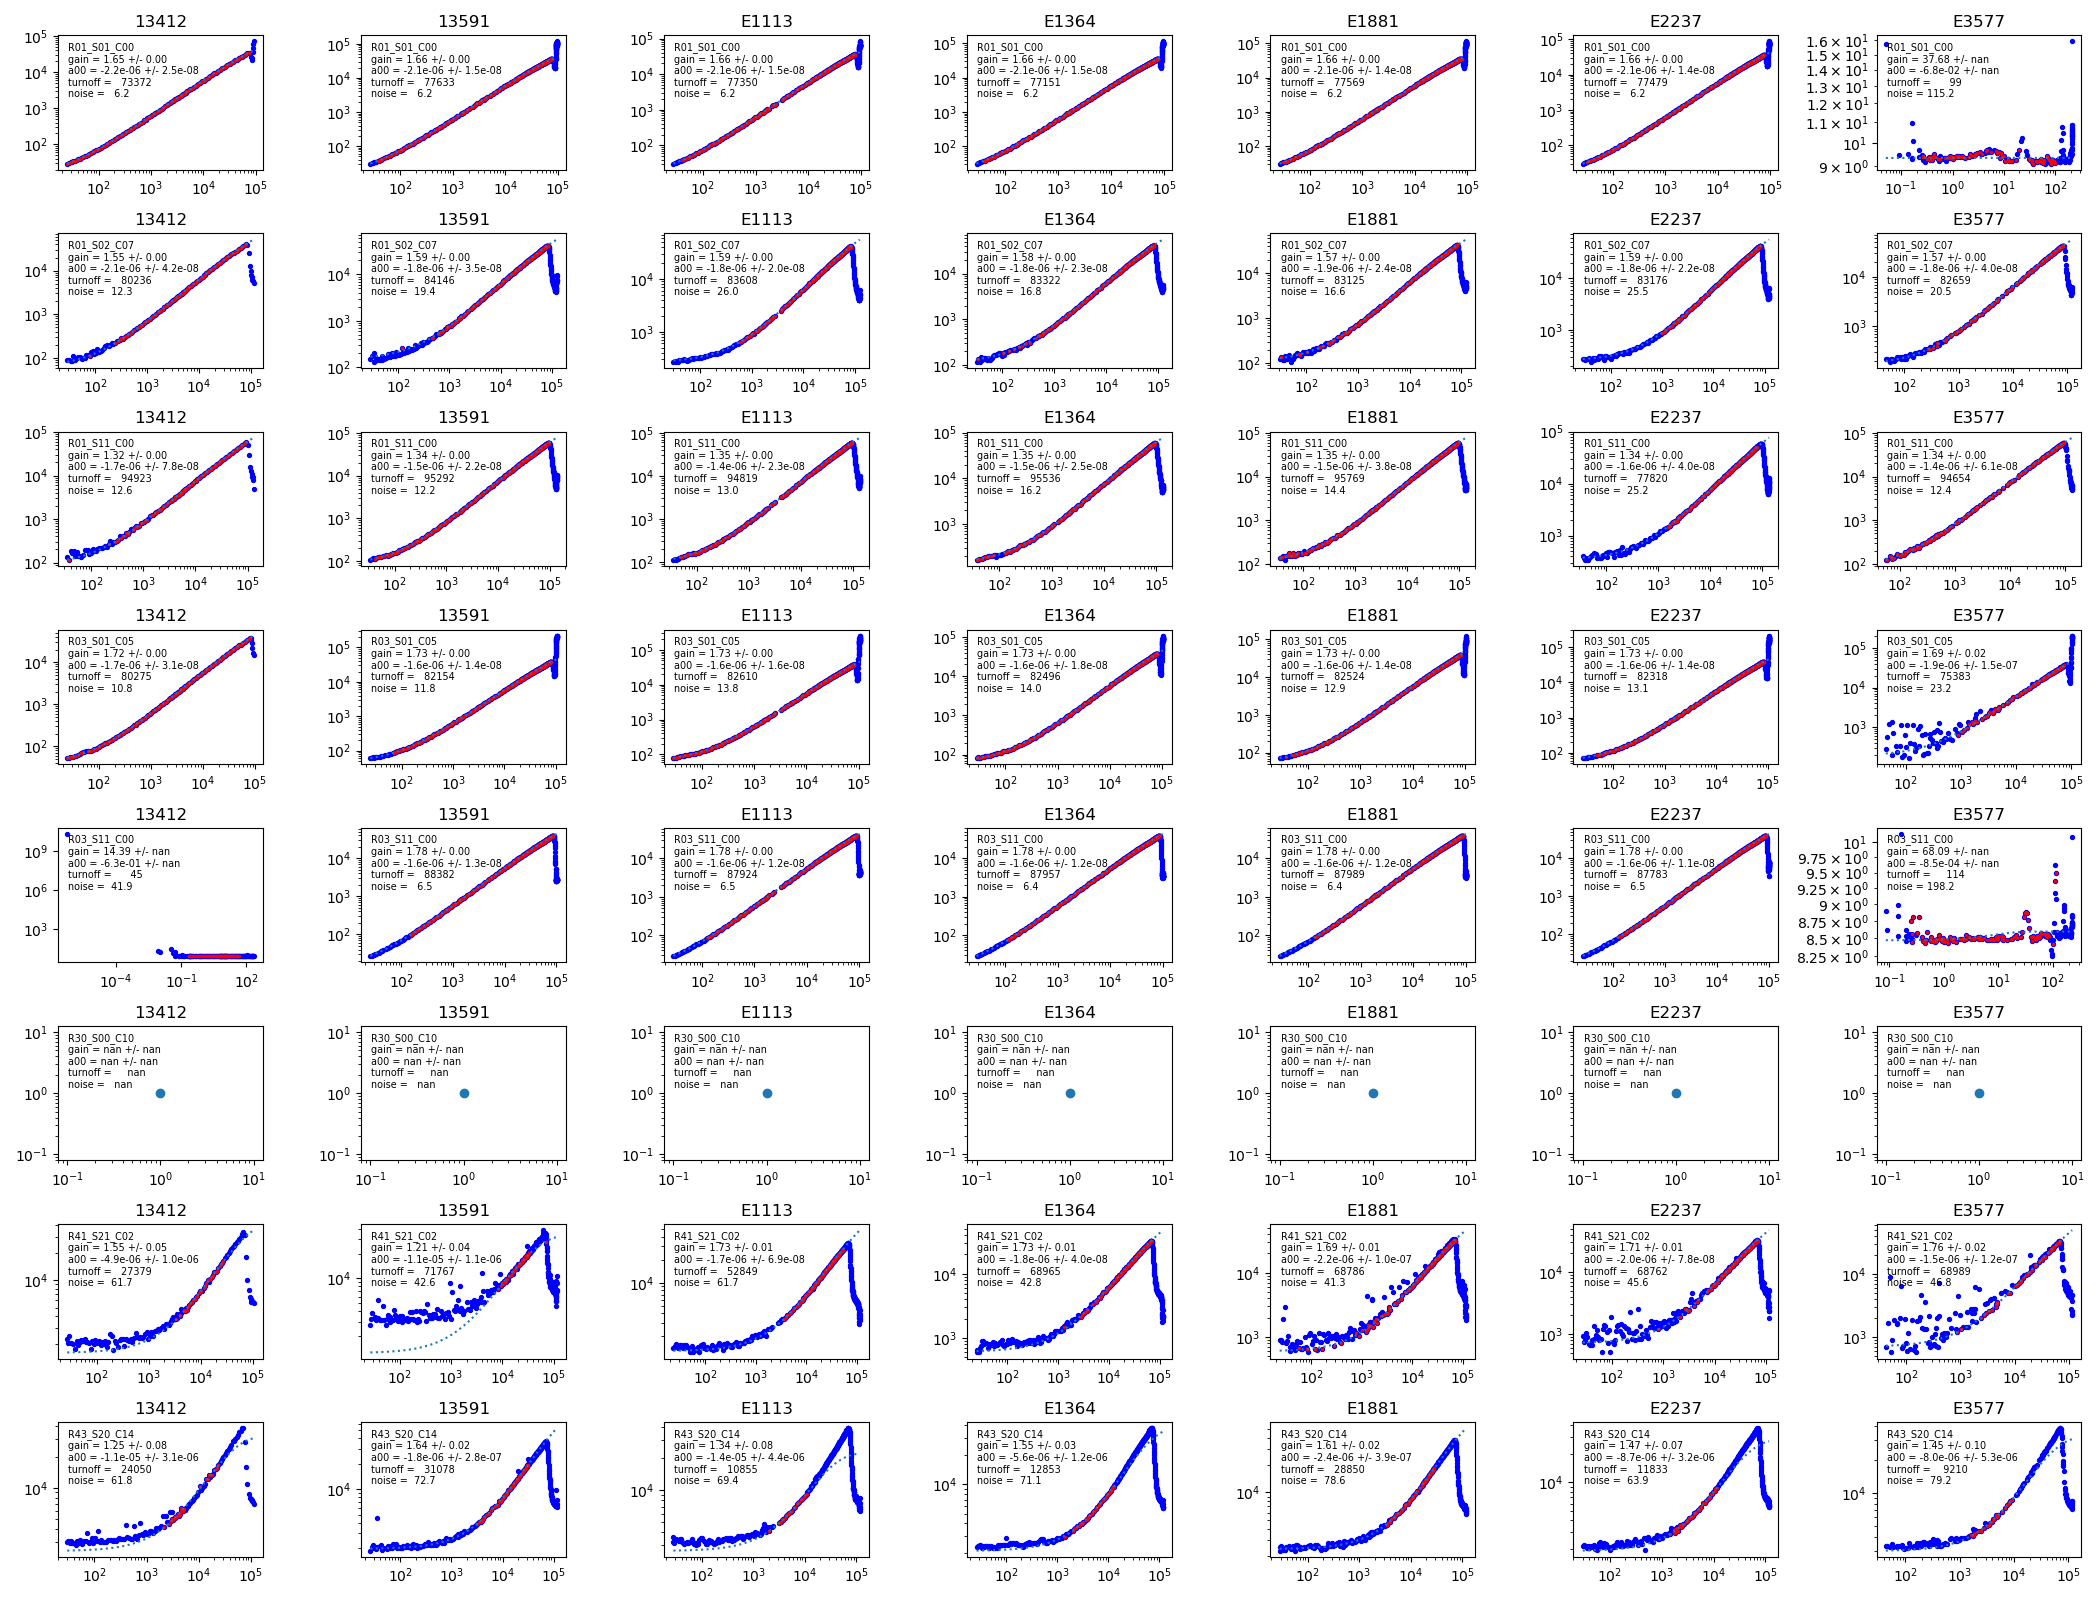
\includegraphics[width=0.95\linewidth]{figures/ptc_badamps.png}
    \caption{PTC plots for amplifiers flagged as potentially problematic, from dense PTC runs}
    \label{fig:ptc-badamps}
\end{figure}

\begin{figure}[ht]
    \centering
    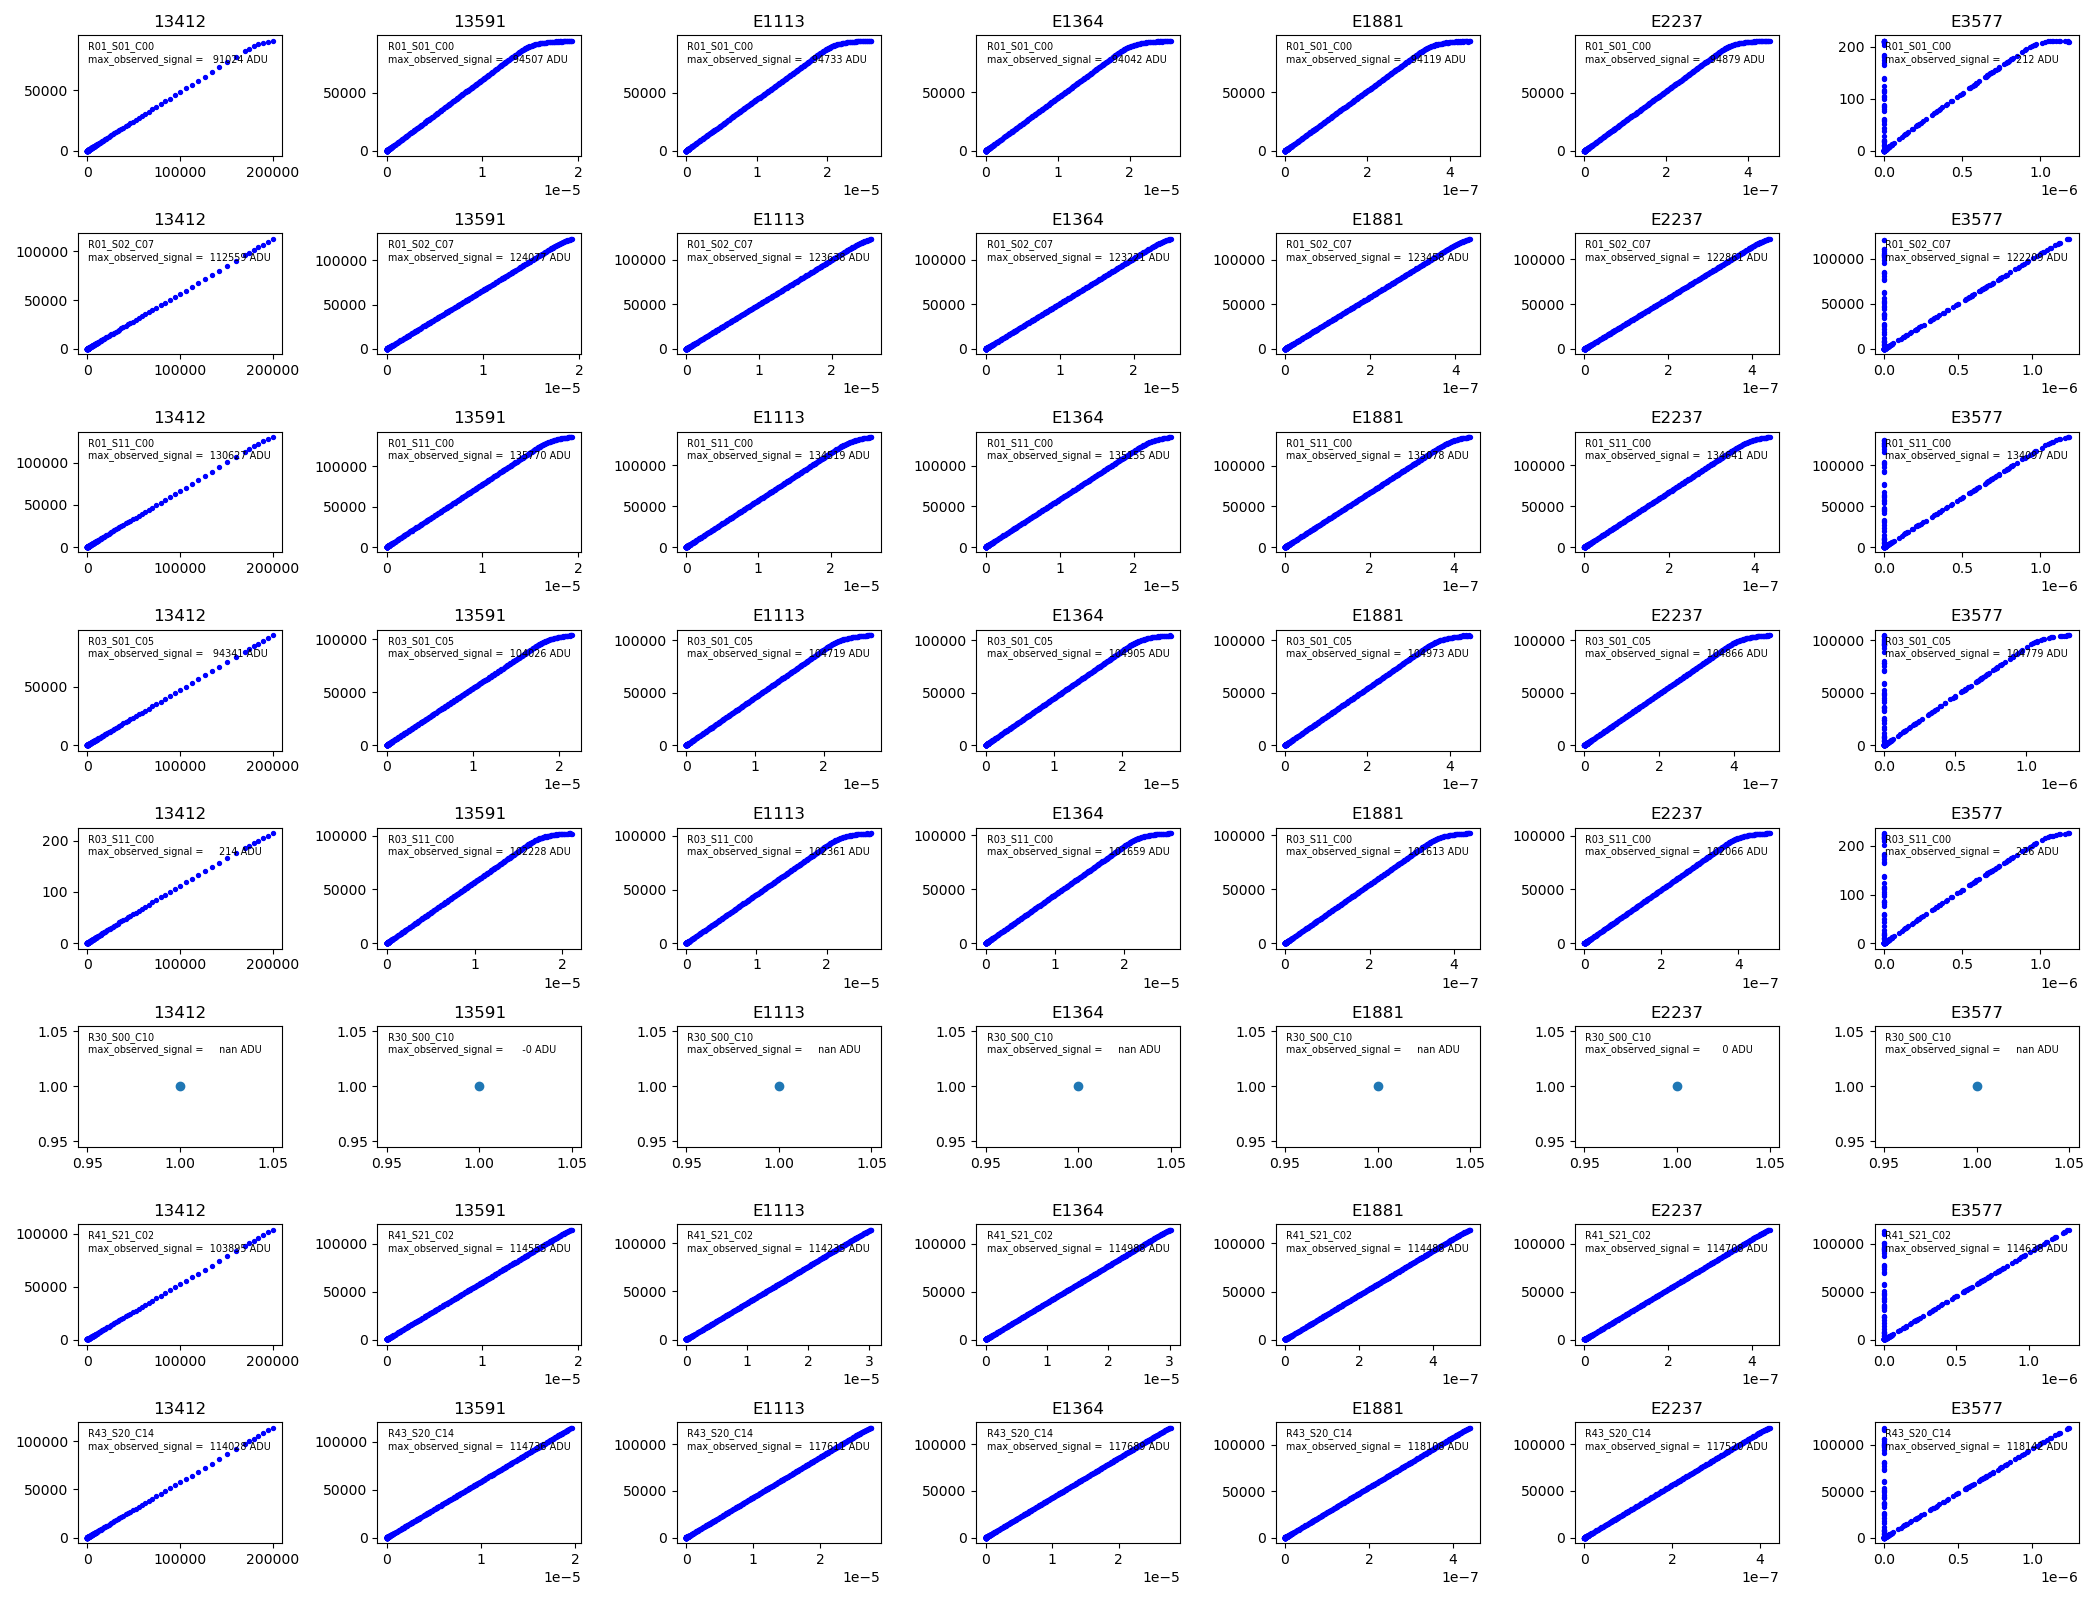
\includegraphics[width=0.95\linewidth]{figures/lin_badamps.png}
    \caption{Linearity plots for amplifiers flagged as potentially problematic, from dense PTC runs}
    \label{fig:lin-badamps}
\end{figure}

\begin{table}[!ht]
    \tiny
    \centering
    \begin{tabular}{|l|l|l|l|l|l|l|l|l|l|l|l|l|}
    \hline
        Channel & Summary & Comments  \\ \hline

R01\_S01\_C00  & Sometimes Dead & Usually OK, turns dead in E3577, previously seen as dead \\ \hline
R01\_S02\_C07  & OK & Noise fluctuates sometimes over $18e^-$ consistent with previous behavior \\ \hline
R01\_S11\_C00  & OK & Noise fluctuates sometimes over $18e^-$ consistent with previous behavior \\ \hline
R03\_S01\_C05  & Sometimes HiNoise & Previously OK,  high noise in E3577 for first time, NEW bad amp \\ \hline
R03\_S11\_C00  & Sometimes Dead & Usually OK, turns dead in E3577, previously seen as dead \\ \hline
R30\_S00\_C10  & Dead & Always dead \\ \hline
R41\_S21\_C02  & HiNoise & Always high noise \\ \hline
R43\_S20\_C14  & HiNoise & Always high noise \\ \hline

    \end{tabular}
    \caption{Table of potentially problematic Science Raft amplifiers, from Runs 6a, 6b, and 7. The Summary column gives the status at the end of Run~7.  Categories are OK, Sometimes HiNoise, Sometimes Dead, HiNoise, Dead. \label{tab:gds_amps}}
\end{table}

Finally, we list problematic Corner raft amplifiers, selected with the same filter.  Three such amplifiers, all in Guide sensors, have been problematic since single CCD testing.  These CCDs were selected for the Guiders due to their single problematic amplifiers, rather than use a fully working Science-grade device. PTC and linearity curves for these channels, for three dense PTC runs, are shown in Figure~\ref{fig:ptclin-badamps-corner}, to classify these channels as either Dead or HiNoise. These three channels are listed in Table~\ref{tab:badamps-corner}

\begin{figure}[ht]
    \centering
    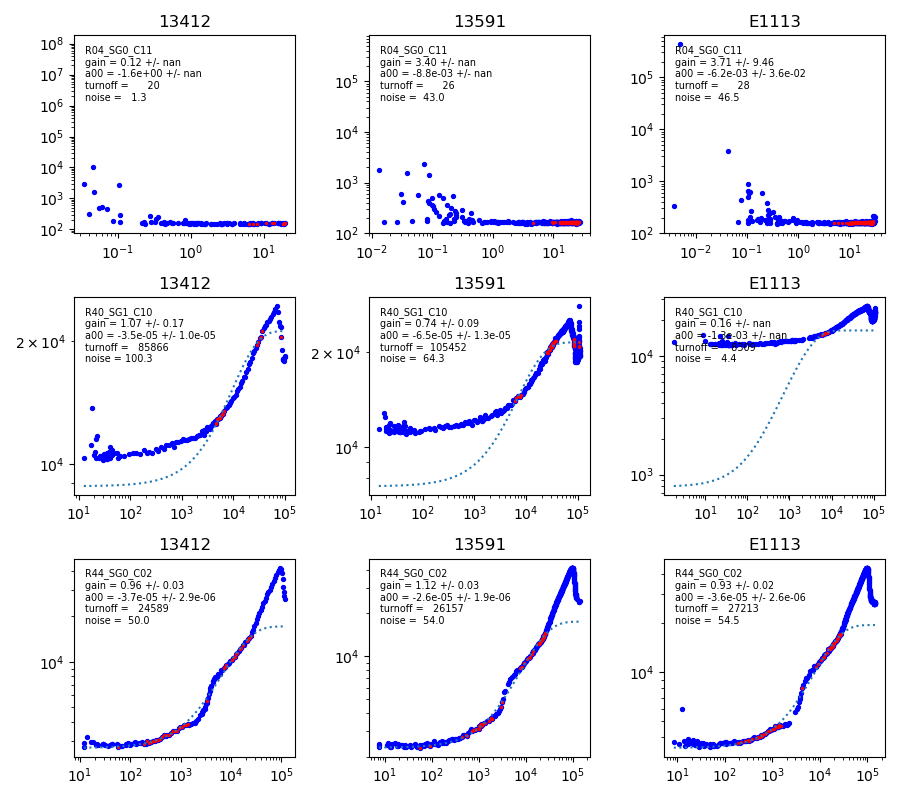
\includegraphics[width=0.45\linewidth]{figures/ptc_badamps_corner.png}
    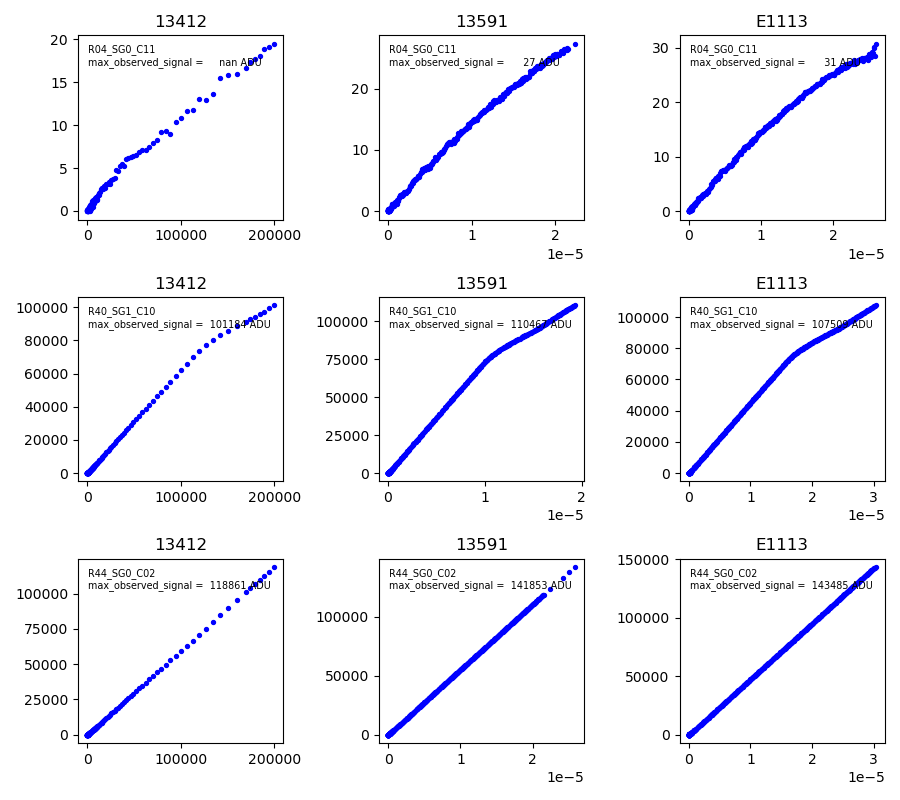
\includegraphics[width=0.45\linewidth]{figures/lin_badamps_corner.png}
    \caption{PTC and Linearity plots for Corner Raft amplifiers flagged as potentially problematic, from Dense PTC runs}
    \label{fig:ptclin-badamps-corner}
\end{figure}

\begin{table}[!ht]
    \tiny
    \centering
    \begin{tabular}{|l|l|l|l|l|l|l|l|l|l|l|l|l|}
    \hline
        Channel & Summary & Comments  \\ \hline

R04\_SG0\_C11  & Dead & Always dead \\ \hline
R40\_SG1\_C10  & HiNoise & Always high noise \\ \hline
R44\_SG0\_C02  & HiNoise & Always high noise\\ \hline

    \end{tabular}
    \caption{Table of problematic Corner Raft amplifiers, from Runs 6a, 6b, and 7. The Summary column gives the status at the end of Run~7. Categories are as in Table~\ref{tab:gds_amps}. \label{tab:badamps-corner}}
\end{table}

\subsection{Defect stability}\label{defect-stability}

EO defect masks are generated for LSSTCam images using two different protocols: one for dark defects, and one for bright defects. Dark defects masks are generated using flat calibrations, by identifying pixels with deviations greater than some threshold from the median flat value. The default dark defect deviation threshold is $\geq 20\%$ deviation from the overall median. Bright defects are identified from elevated dark current. The default bright defect condition is $\geq$5\,e-/pix/s.

As shown in Table~\ref{table:FinalChar-paramTable}, the median number of defects in an amplifier is $\leq 10$, or $\sim0.001\%$ of an amplifier for both e2v and ITL sensors. This contribution is extremely small relative to the useful pixels in a given amplifier. Studying any temporal dependence of defect masks on the amplifiers would be worthwhile.  %, and how static the bright and dark defects are across sensors of interest.

\begin{figure}[ht]
    \centering
    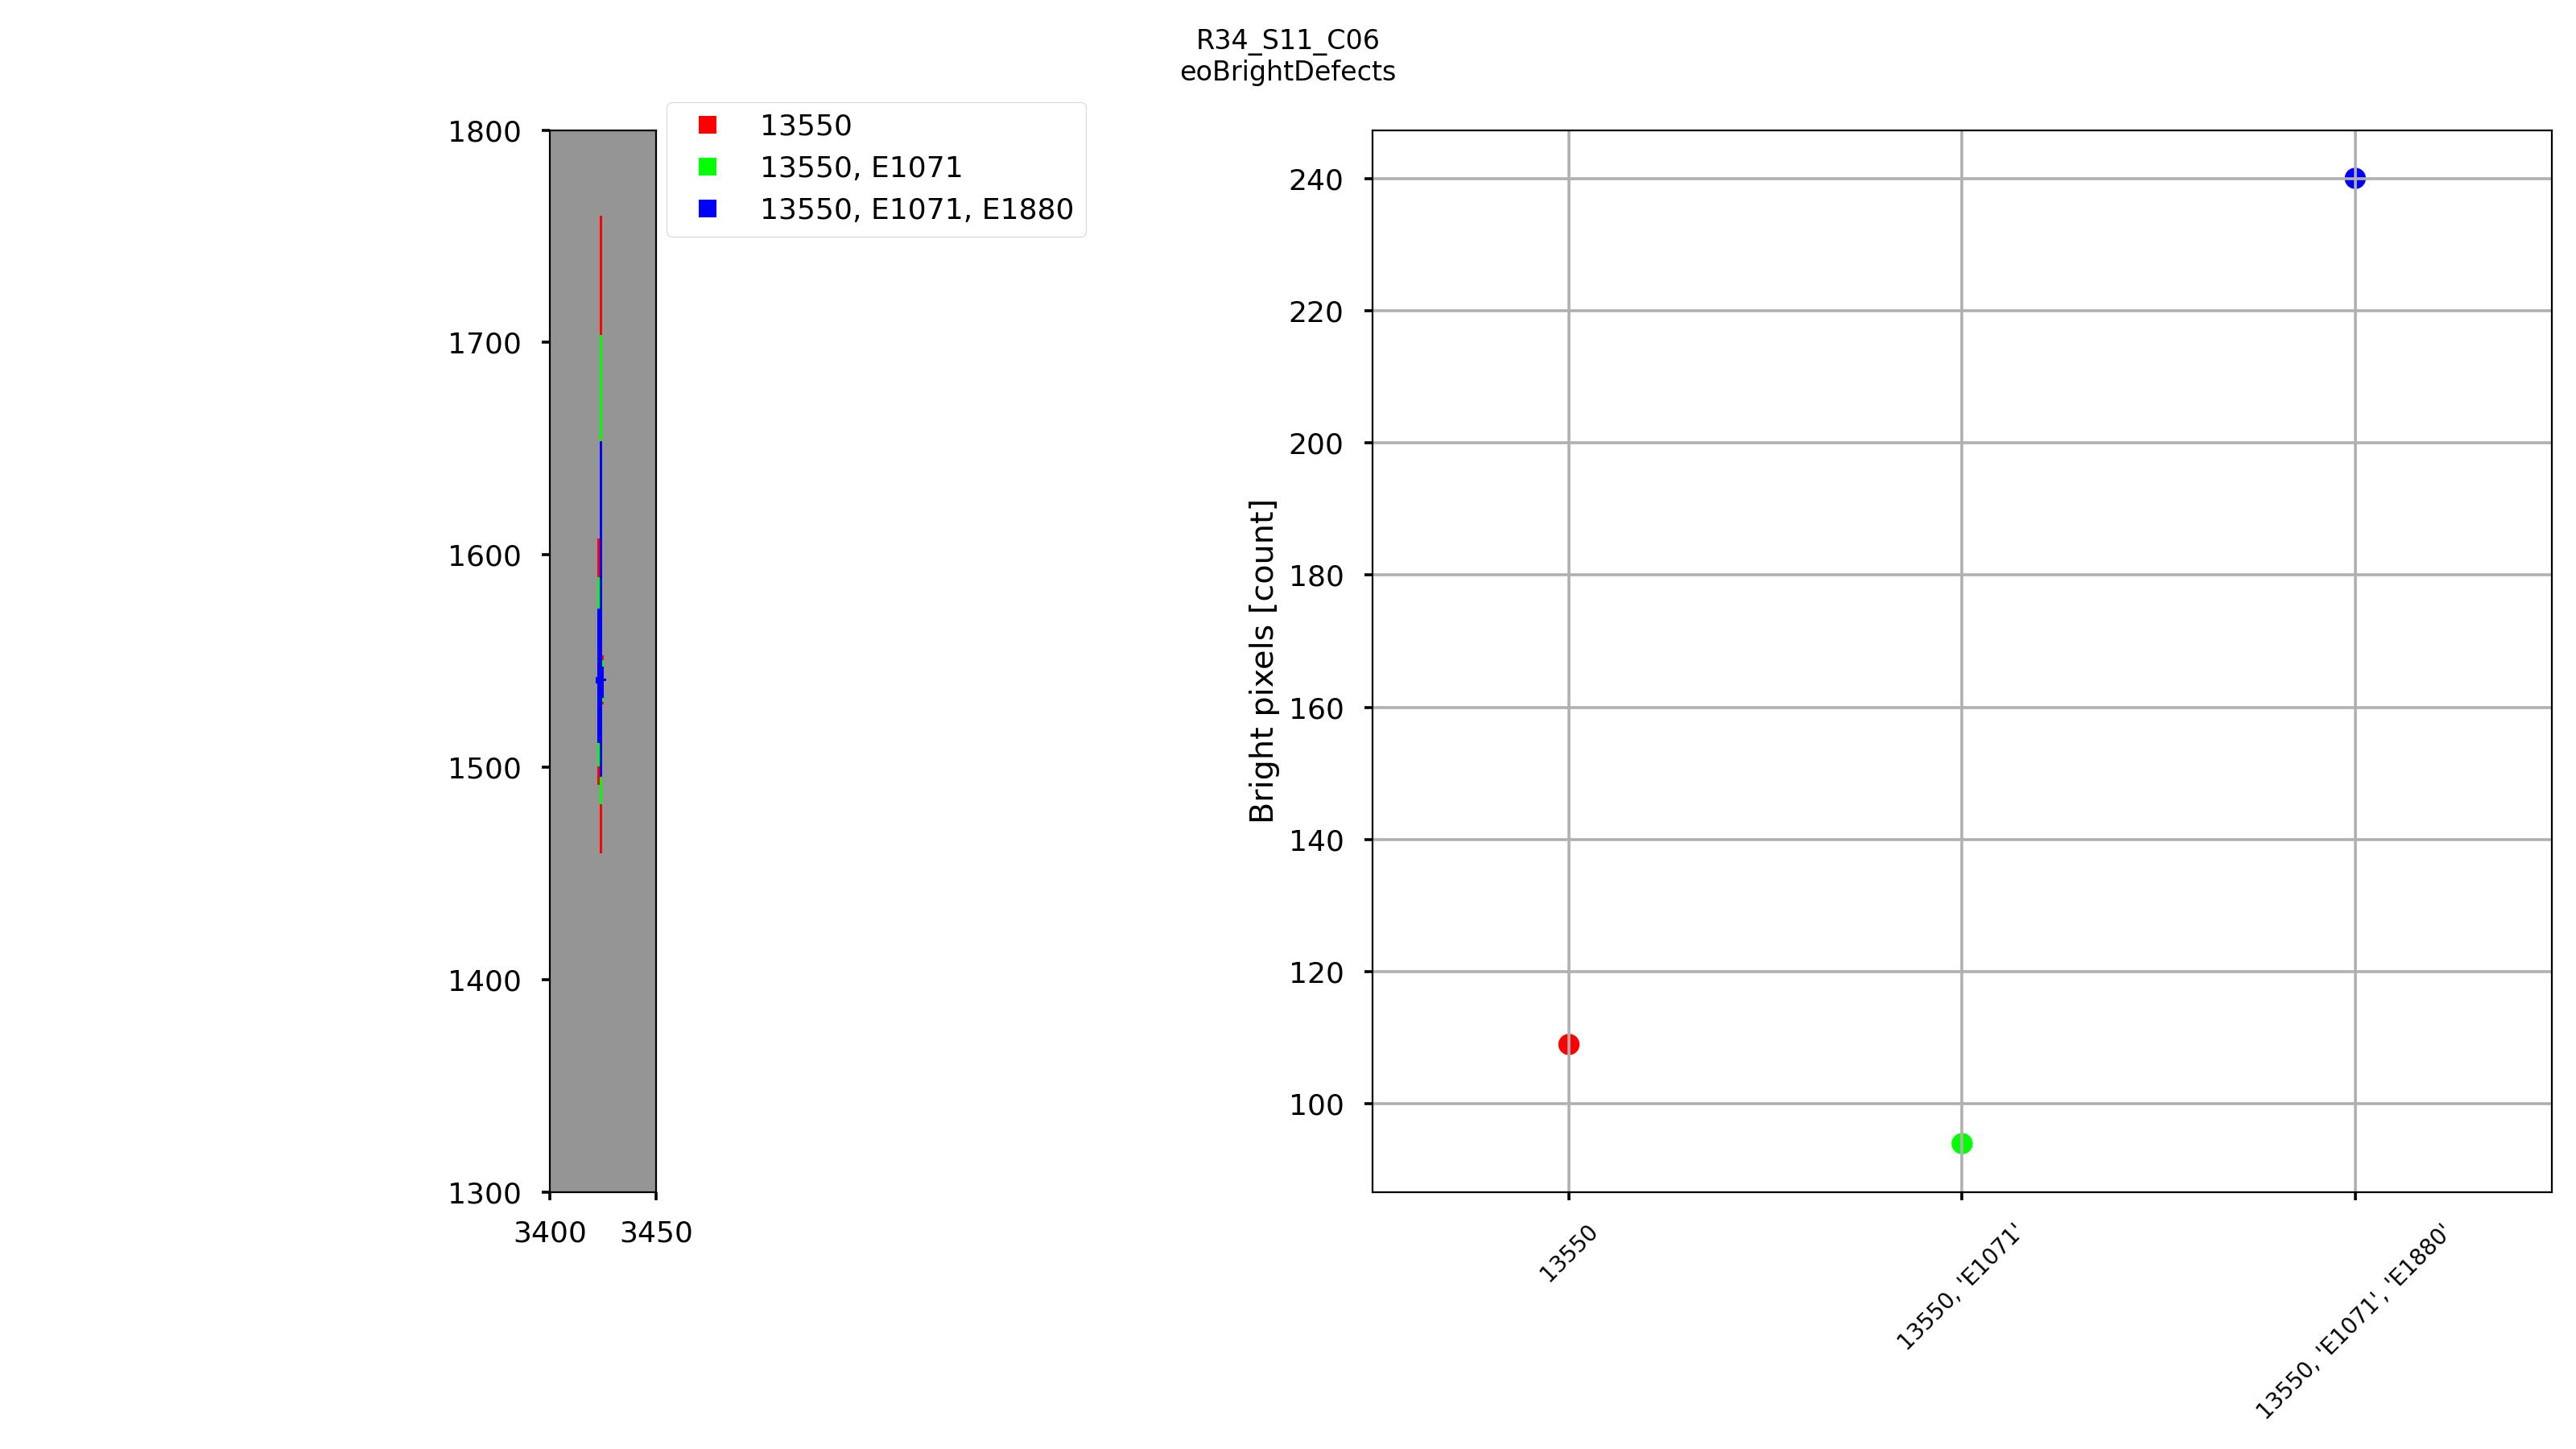
\includegraphics[width=\linewidth]{figures/R34_S11_C06(1).jpg}
    \caption{Bright defect stability over a small region of R34\_S11\_C06. Notably, this bright defect decreased in size as testing progressed from Run 6 $\rightarrow$ initial Run 7 $\rightarrow$ final Run 7. Left: A small region of R34\_S11\_C06, where the coordinates shown are in detector space for R34\_S11. the colored regions denote different bright defect masks. Mask bits common to Run 6, early Run 7, and final Run 7 runs are shown in blue. Mask bits common to Run 6 and early Run 7 runs are shown in green. Mask bits common to Run 6 only are shown in red. Right: The defect count for the different mask planes over R34\_S11\_C06. The counts shown here are for the entire segment, not the subset of the segment shown on the left.}
    \label{fig:BrightDefectStability}
\end{figure}

To measure differences between defect masks from different runs, we can compare the resulting defect masks using binary composition. For a defect mask on an amplifier, we consider individual bright/dark defect masks from individual runs, assigning a value of $1$ to each pixel that is masked. Unmasked pixels are assigned a value of $0$.

%% Maybe add a figure/cartoon here that shows the process of combining the different masks

Each individual defect mask can be scaled by $2^{n}$, where $\{n:0,1,2,3,... \}$ denotes an index associated with a defect mask (from Run 6, early Run 7, or late Run 7). These individual defect masks are added together to created a composite defect mask, ranging in value from $[0,2^{n}-1]$, with each bit value becoming associated with a different composition of mask planes. By comparing the defect mask bit values of different masks, it is then possible to recover on the segment level the uniqueness and stability of a defect mask by comparing the composition bit values to the mask indices. For a completely unmasked segment, the defect mask will be composed of 0's only. For a static defect mask, the composite defect mask will be composed of bit values 0 and $2^n$ only. This analysis is performed on dark and bright defects for Run 6, initial Run 7 and final Run 7 data (see Table \ref{table:defectStability:measurements}).

\begin{table}[ht]
\centering
\begin{tabular}{|ccc|}
\hline
\multicolumn{3}{|c|}{Both bright and dark defects}                      \\ \hline
\multicolumn{1}{|c|}{}    & \multicolumn{1}{c|}{Unmasked} & Static mask \\ \hline
\multicolumn{1}{|c|}{E2V} & \multicolumn{1}{c|}{17.7885}  & 57.7991     \\ \hline
\multicolumn{1}{|c|}{ITL} & \multicolumn{1}{c|}{6.0764}   & 33.1597     \\ \hline
\multicolumn{3}{|c|}{Bright defects only}                               \\ \hline
\multicolumn{1}{|c|}{}    & \multicolumn{1}{c|}{Unmasked} & Static mask \\ \hline
\multicolumn{1}{|c|}{E2V} & \multicolumn{1}{c|}{72.5427}  & 93.6432     \\ \hline
\multicolumn{1}{|c|}{ITL} & \multicolumn{1}{c|}{50.0000}  & 82.3785     \\ \hline
\multicolumn{3}{|c|}{Dark defects only}                                 \\ \hline
\multicolumn{1}{|c|}{}    & \multicolumn{1}{c|}{Unmasked} & Static mask \\ \hline
\multicolumn{1}{|c|}{E2V} & \multicolumn{1}{c|}{23.9316}  & 60.5769     \\ \hline
\multicolumn{1}{|c|}{ITL} & \multicolumn{1}{c|}{11.6319}  & 39.5833     \\ \hline
\end{tabular}
\caption{Measurements of the percentages of science sensor amplifiers that meet different masking criteria, when compared across 13550 (Run 6), E1071 (Run 7 initial), and E1880 (Run 7 final). For a completely unmasked segment, the defect mask will be composed of 0's only. For a static defect mask, the composite defect mask will be composed of bit values 0 and $2^3-1=7$ only. For this tabulation we removed a 9-pixel border from each dark mask to remove the edge response from the dark defect data set. Other masking configurations were set to the LSSTCam defaults.}
\label{table:defectStability:measurements}
\end{table}

\subsubsection{Bright defects}

Bright defects are found to be stable and rare in the LSSTCam focal plane. Across detector types, 93\% of e2v detectors show a static bright defect mask. For e2v sensors that had changes in bright defects, R30 dominated the subgroup with 17 amplifiers (or 11.8\% of amplifiers on the raft) with a dynamic bright defect mask. Bright pixel masks of ITL sensors are more dynamic than for e2v sensors, with 18\% having changes in their bright defect masks. The most dynamic bright defect masks were for R10\_S02 and R10\_S10, which each have nine amplifiers with a dynamic bright defect mask.


\begin{figure}[ht]
    \centering
    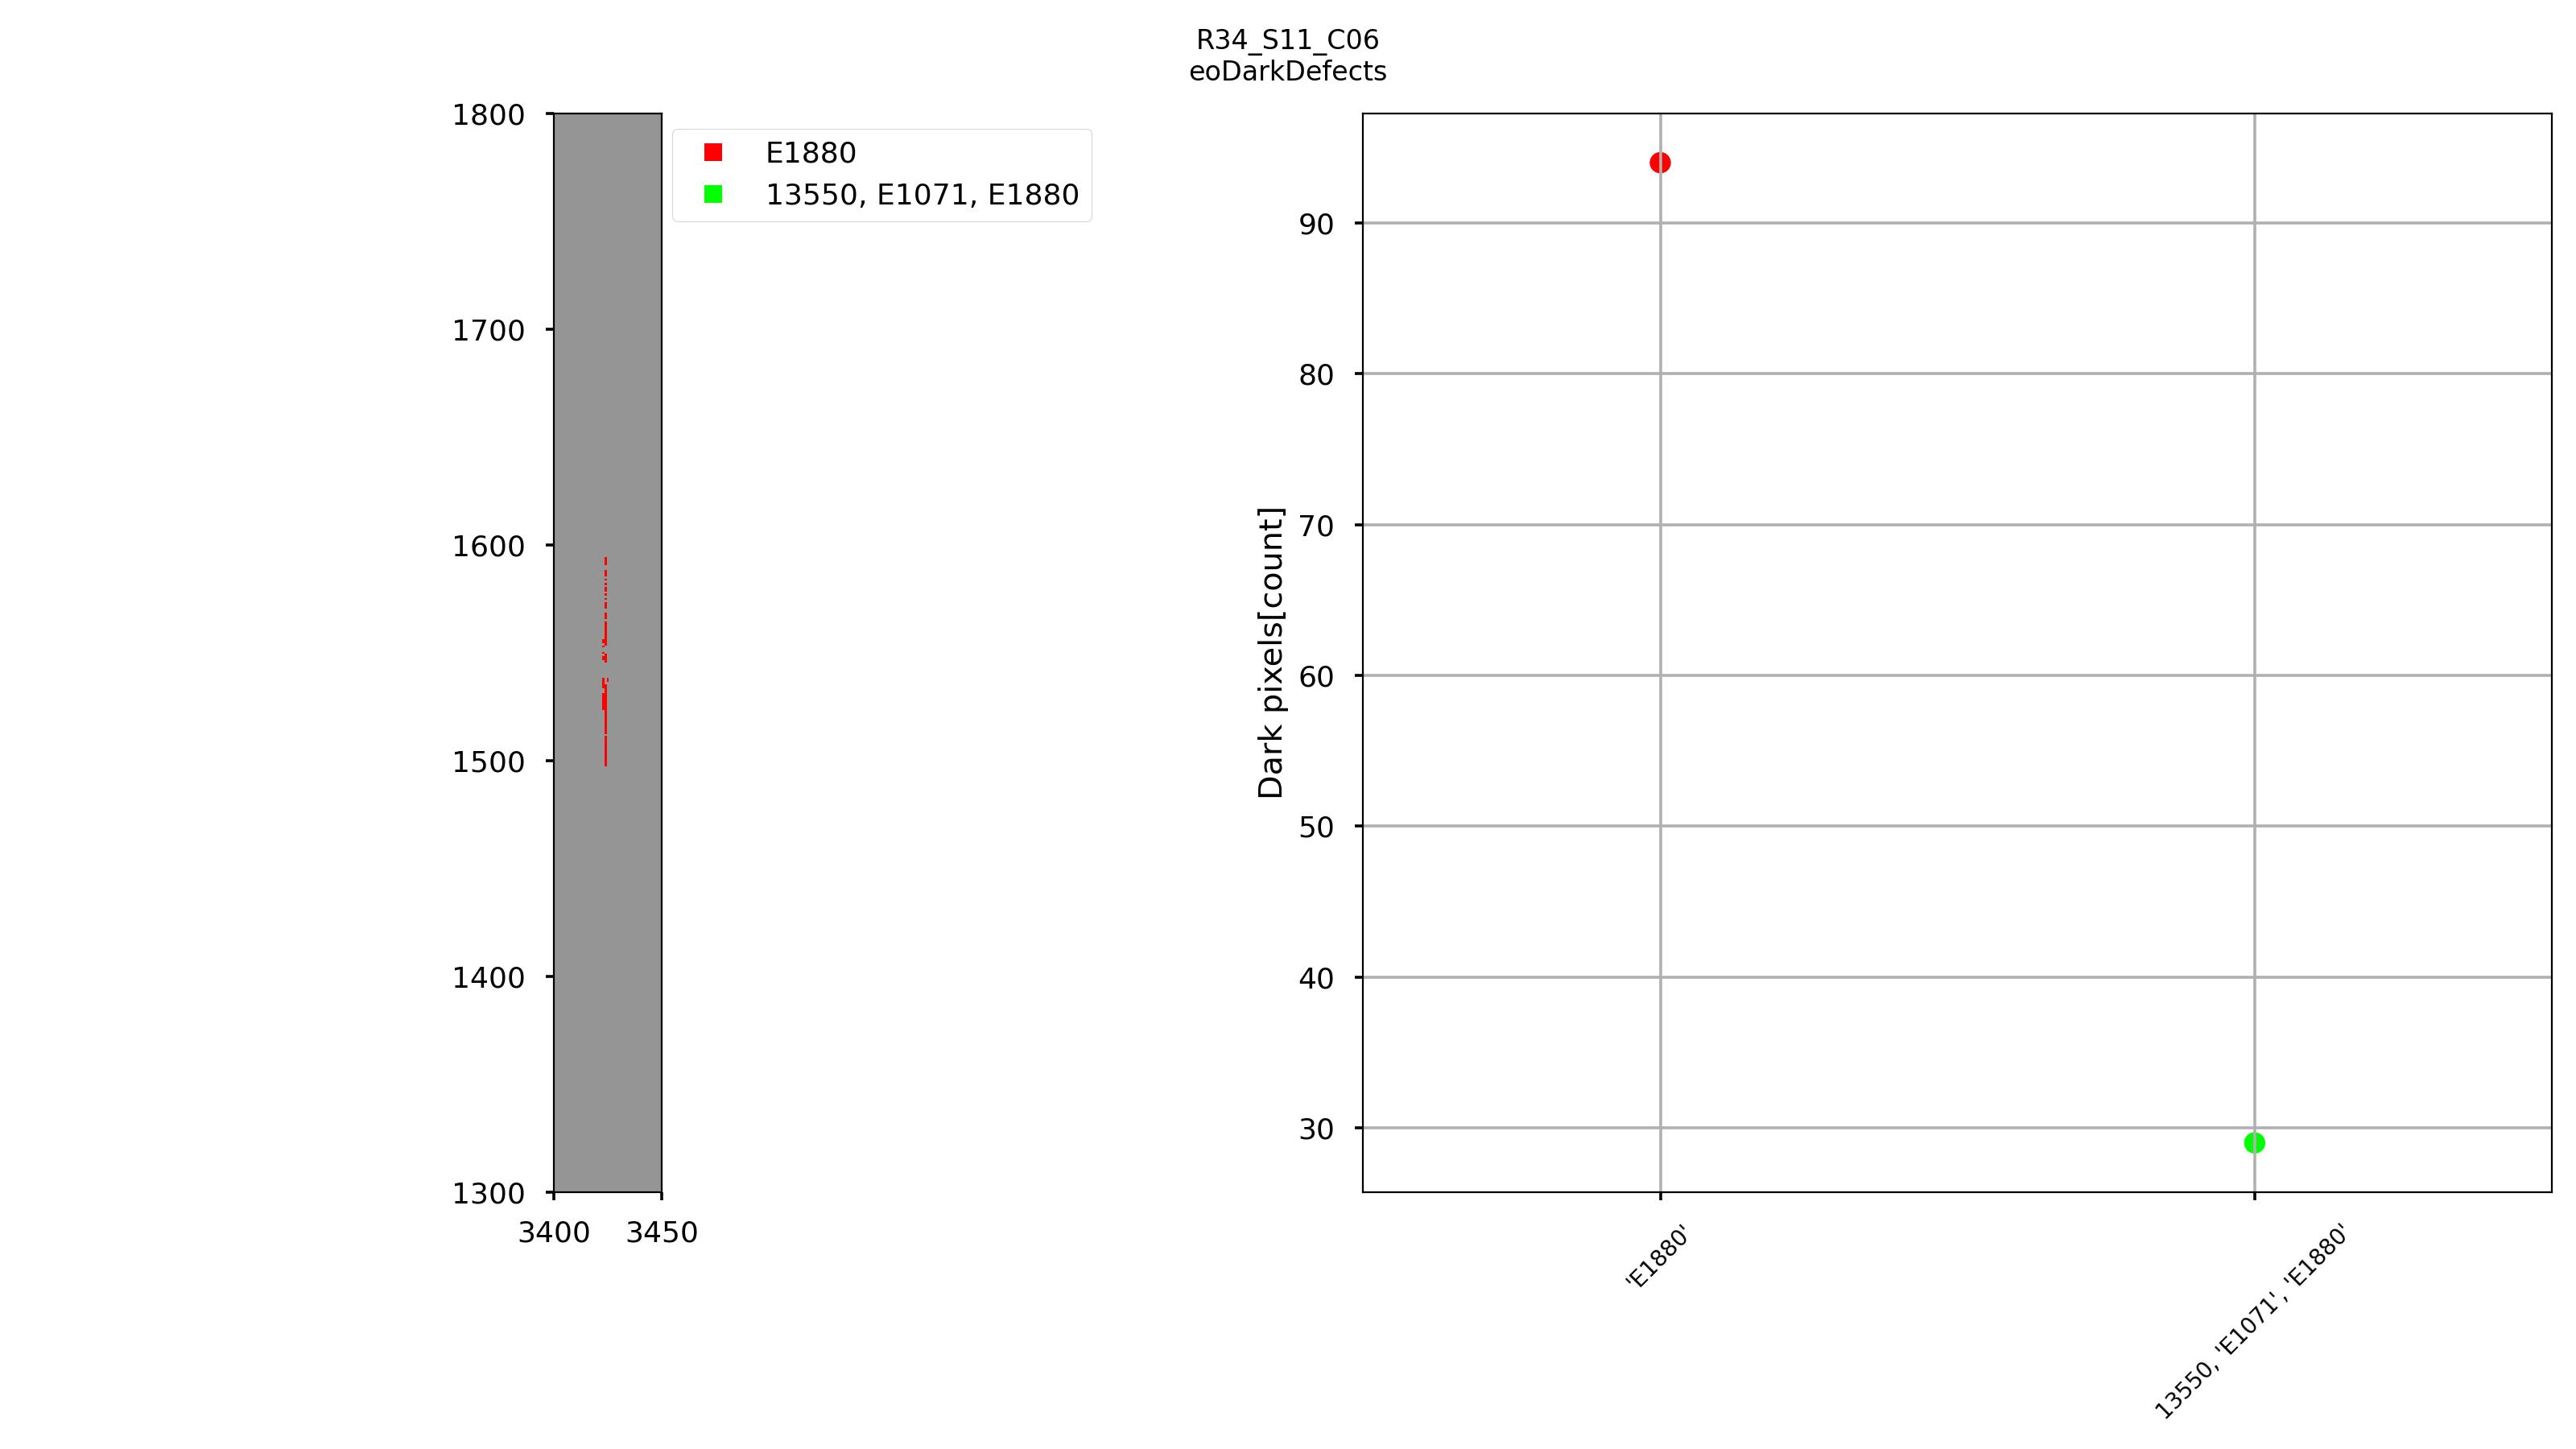
\includegraphics[width=\linewidth]{figures/R34_S11_C06(2).jpg}
    \caption{Dark defect stability over a small region of R34\_S11\_C06. Notably, this dark defect developed in the final record run of Run 7. Left: A small region of R34\_S11\_C06, where the coordinates shown are in detector space for R34\_S11. The colored regions denote different dark defect masks. Mask bits unique to final Run 7 is shown in red. Right: The defect count for the different mask planes over R34\_S11\_C06. The counts shown here are for the entire segment, not the subset of the segment shown on the left.}
    \label{fig:DarkDefectStability}
\end{figure}

\subsubsection{Dark defects}

Dark defects are less stable and more abundant across the focal plane than bright defects. Across detector types, 60\% of e2v detectors require a static bright defect mask. Dynamic e2v dark defect masks are distributed across the entire focal plane, with every e2v sensor registering a dynamic (i.e., time dependent) e2v dark defect mask across 13550, E1071, and E1880. Among dynamic e2v sensors, R34 dominated the subgroup, with R34\_S02, R34\_S12, and R34\_S22 registering 15 amplifiers with dynamic dark defect masks. ITL sensors are once again more dynamic than e2v sensors, with 39\% showing a static dark defect mask. The ITL non-static dark defect mask is present in every sensor across the focal plane, with sensors R01\_S12, R01\_S22, R41\_S02, R41\_S12, and R41\_S20 measuring a dynamic dark defect mask on every amplifier.


% Plot here of a particularly interesting bright defect mask that changes substantially

\subsection{Bias stability}\label{sec:bias-stability-2}

We have found bias instabilities, typically above the 1 ADU level, for a number of CCDs in the focal plane, both ITL and e2v. Two main kinds of instability are observed:

\begin{enumerate}
\tightlist
\item
  ITL bias jumps: large variations of the column-wise structure from
  exposure to exposure.
\item
  e2v yellow corners: a residual 2D shape of the bias even after
  2D-overscan correction. These residuals depend on the acquisition
  sequence and the exposure time, and the enhancement is greatest near the readout nodes (hence `yellow corner').
\end{enumerate}

Both issues were observed and deeply studied in Run 6 EO data. The ITL
issue is believed to be random phase shifts in clocks due to the fact that REBs convert their natural clock units of 6.4ns to an artificial one of 10ns. In this conversion, there could be ambiguity in timing with respect to the natural clock. We tried to mitigate the e2v issue by
optimizing the acquisition configuration in Run 7.

For the baseline acquisition configuration (see Section~\ref{conclusions}), three
relevant stability runs were recorded:

\begin{enumerate}
\tightlist
\item
  Run E2136: 15\,s darks with some very long delays throughout the run
\item
  Run E2236: 50 15\,s darks, 50 biases recorded with 30\,s delays between
  exposures
\item
  Run E2330: 15\,s and 30\,s darks with variable delays between exposures
\end{enumerate}

To analyze these runs for bias instability, the {\tt eo\_pipe} bias
stability task is used.  For the ISR part, a serial
%(\textquotesingle mean\phantomsection\label{per_row}{per\_row}\textquotesingle)
(`mean\_per\_row')
overscan correction is applied. The final data product of the task is the
mean of the per-amplifier science image over the full set of exposures
of the run. Two typical examples from Run E2136 are shown in Figure~\ref{fig:bias-instability}. In the stable case, the variations are typically at the 0.1 ADU
level; in the unstable case, the variations range up to 4 ADUs.

\begin{figure}[ht]
\centering
\begin{minipage}[b]{0.5\textwidth}
\centering
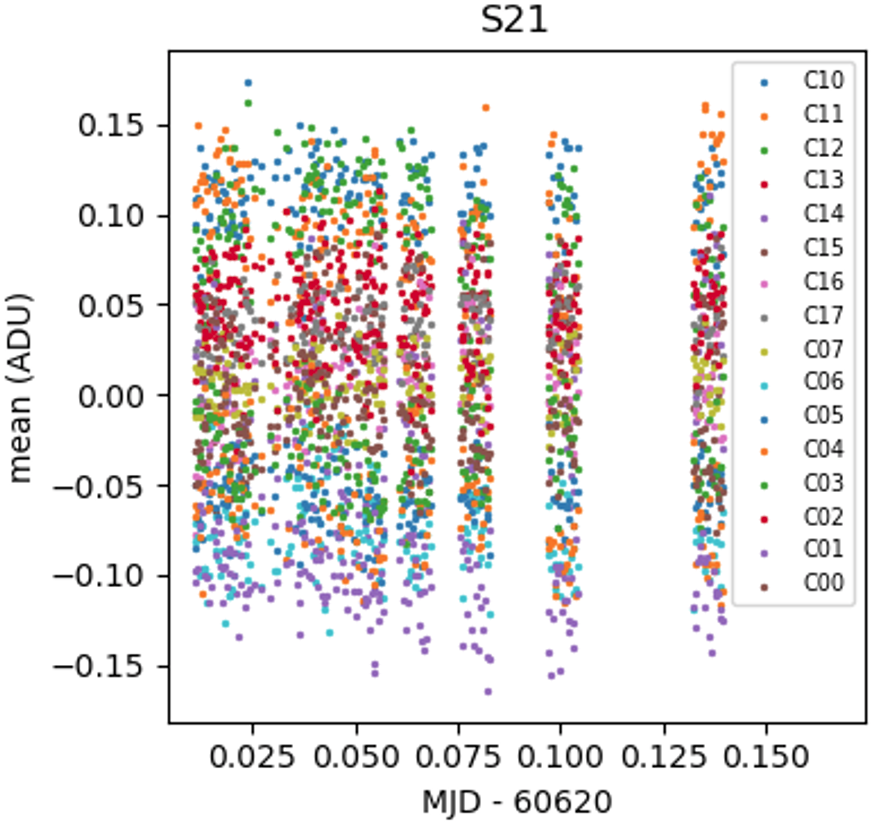
\includegraphics[width=\textwidth]{figures/E2136_R21_S21.png}
\end{minipage}
%\hfill
\begin{minipage}[b]{0.45\textwidth}
\centering
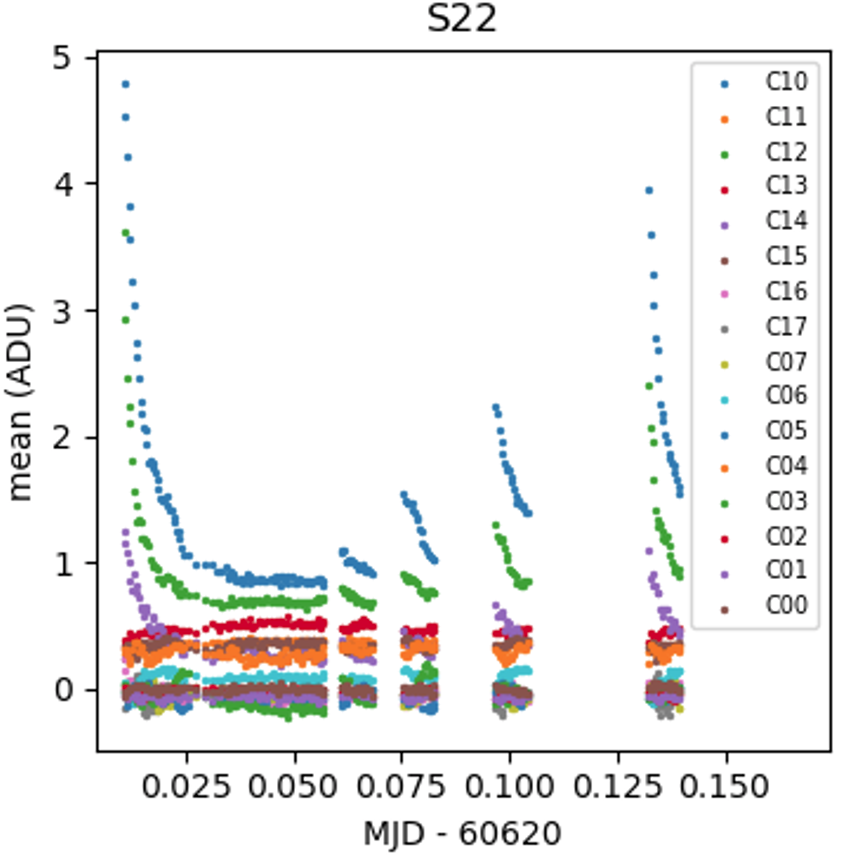
\includegraphics[width=\textwidth]{figures/E2136_R23_S22.png}
\end{minipage}
\caption{(left) Stable case for bias (R21\_S21); (right) Unstable case (R23\_S22)}
\label{fig:bias-instability}
\end{figure}


A comparison of the results for an unstable e2v CCD (R33\_S02) is shown in Figure~\ref{fig:r33_s02_bias} for the
three runs. It must be noted that this instability can be greatly reduced at the software level with the use of a two-dimensional overscan correction (serial and parallel), as illustrated in
the last panel of Figure~\ref{fig:r33_s02_bias}, but this approach brings disadvantages whose impact needs to be estimated.

\begin{figure}[htbp]
\centering
\begin{minipage}[b]{0.45\textwidth}
    \centering
    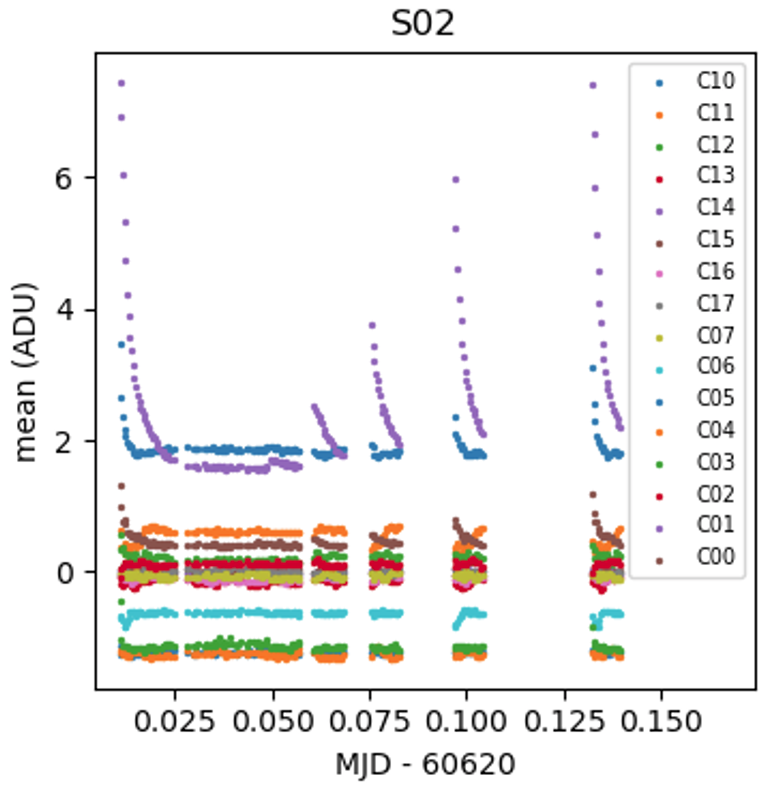
\includegraphics[width=\textwidth]{figures/E2136_R33_S02.png}
    %\caption{Run E2136, R33\_S02}
\end{minipage}
\hspace{0.05\textwidth}
\begin{minipage}[b]{0.45\textwidth}
    \centering
    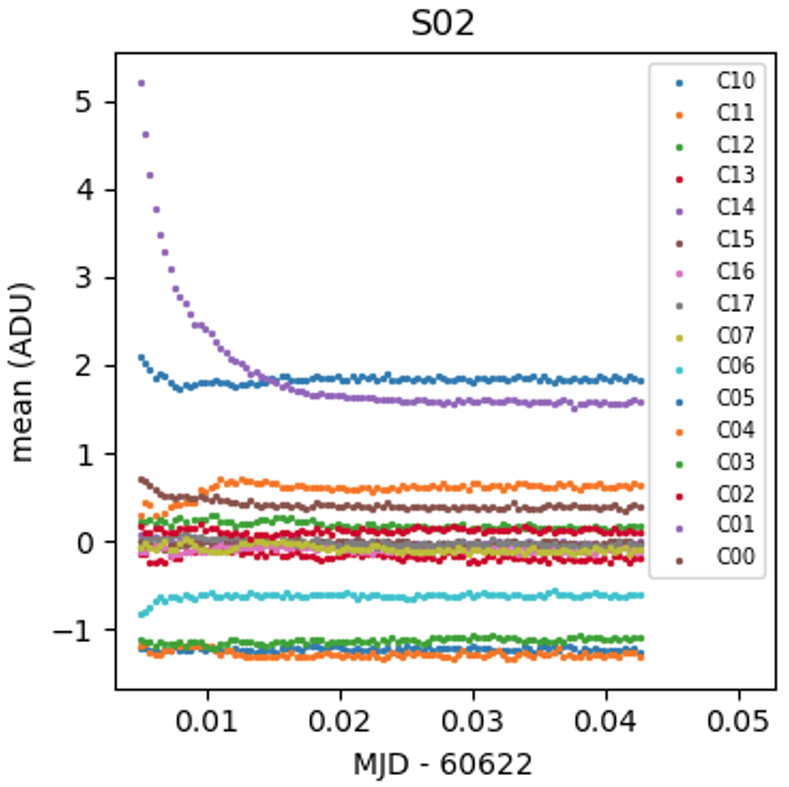
\includegraphics[width=\textwidth]{figures/E2236_R33_S02.png}
    %\caption{Run E2236, R33\_S02}
\end{minipage}

\vspace{0.05\textwidth}

\begin{minipage}[b]{0.45\textwidth}
    \centering
    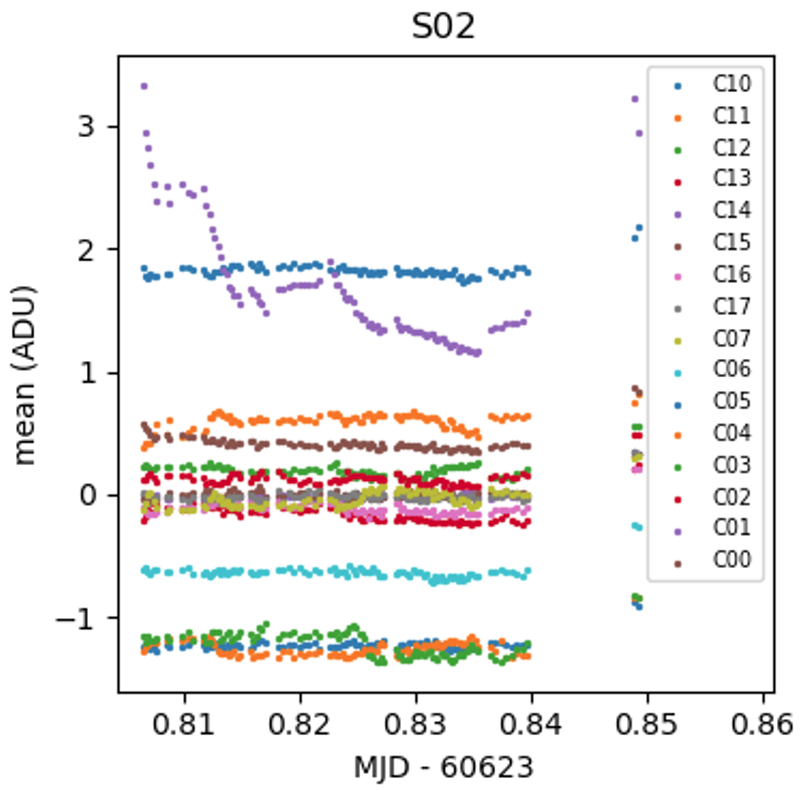
\includegraphics[width=\textwidth]{figures/E2330_R33_S02.png}
    %\caption{Run E2330, R33\_S02}
\end{minipage}
\hspace{0.05\textwidth}
\hfill
\begin{minipage}[b]{0.45\textwidth}
    \centering
    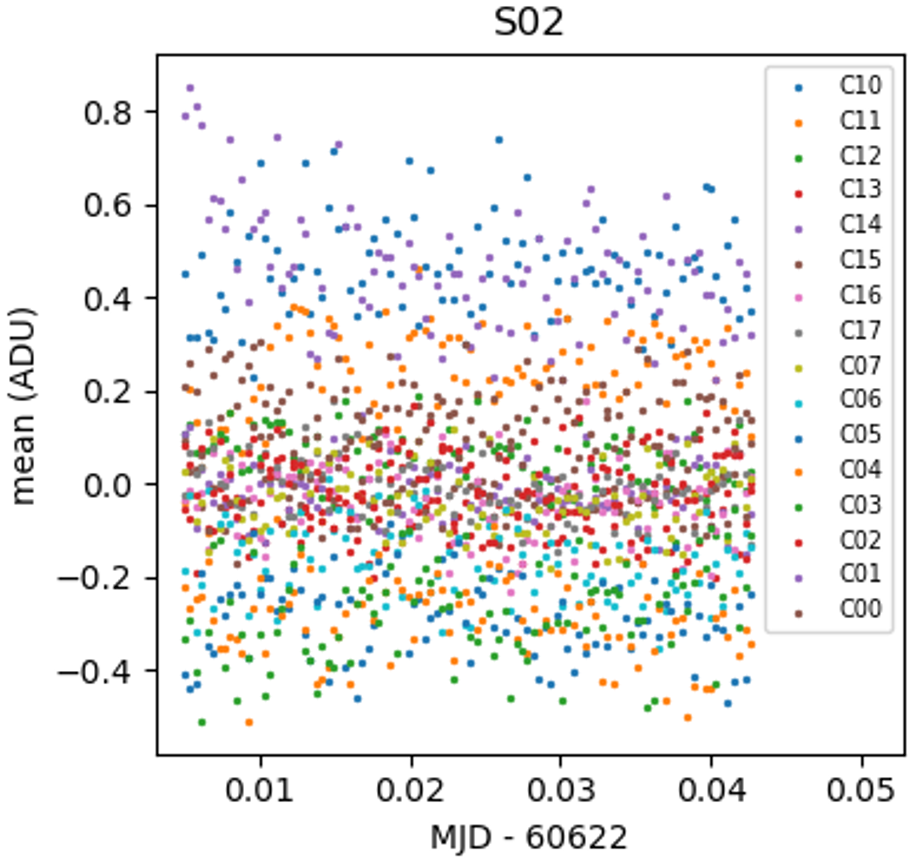
\includegraphics[width=\textwidth]{figures/E2236_2D_R33_S02.png}
    % kept as a blank cell
\end{minipage}
\caption{Bias level variations for R33\_S02, an unstable e2v CCD, for three runs:  (upper left) E2136, (upper right) E2236, (lower left) E2330.  The segments C01 and C10 are most strongly variable in each run.  Note that the range of the time axis is different in each plot. The lower right panel shows the variations for the run E2236 with the parallel overscan correction applied.}
\label{fig:r33_s02_bias}
\end{figure}

To highlight the 2D shape differences in e2v bias instability, a 2D-overscan correction
is applied. A few exposures illustrating the variations of the 2D shape
for the same unstable CCD R33\_S02 are shown in Figures~\ref{fig:r33_s02_1880}--\ref{fig:r33_s02_2136_delay}. The 2D shape of the image in
amplifier C01 is different in the 3 cases.

\begin{figure}[htbp]
\centering
\begin{minipage}{0.45\textwidth}
    \centering
    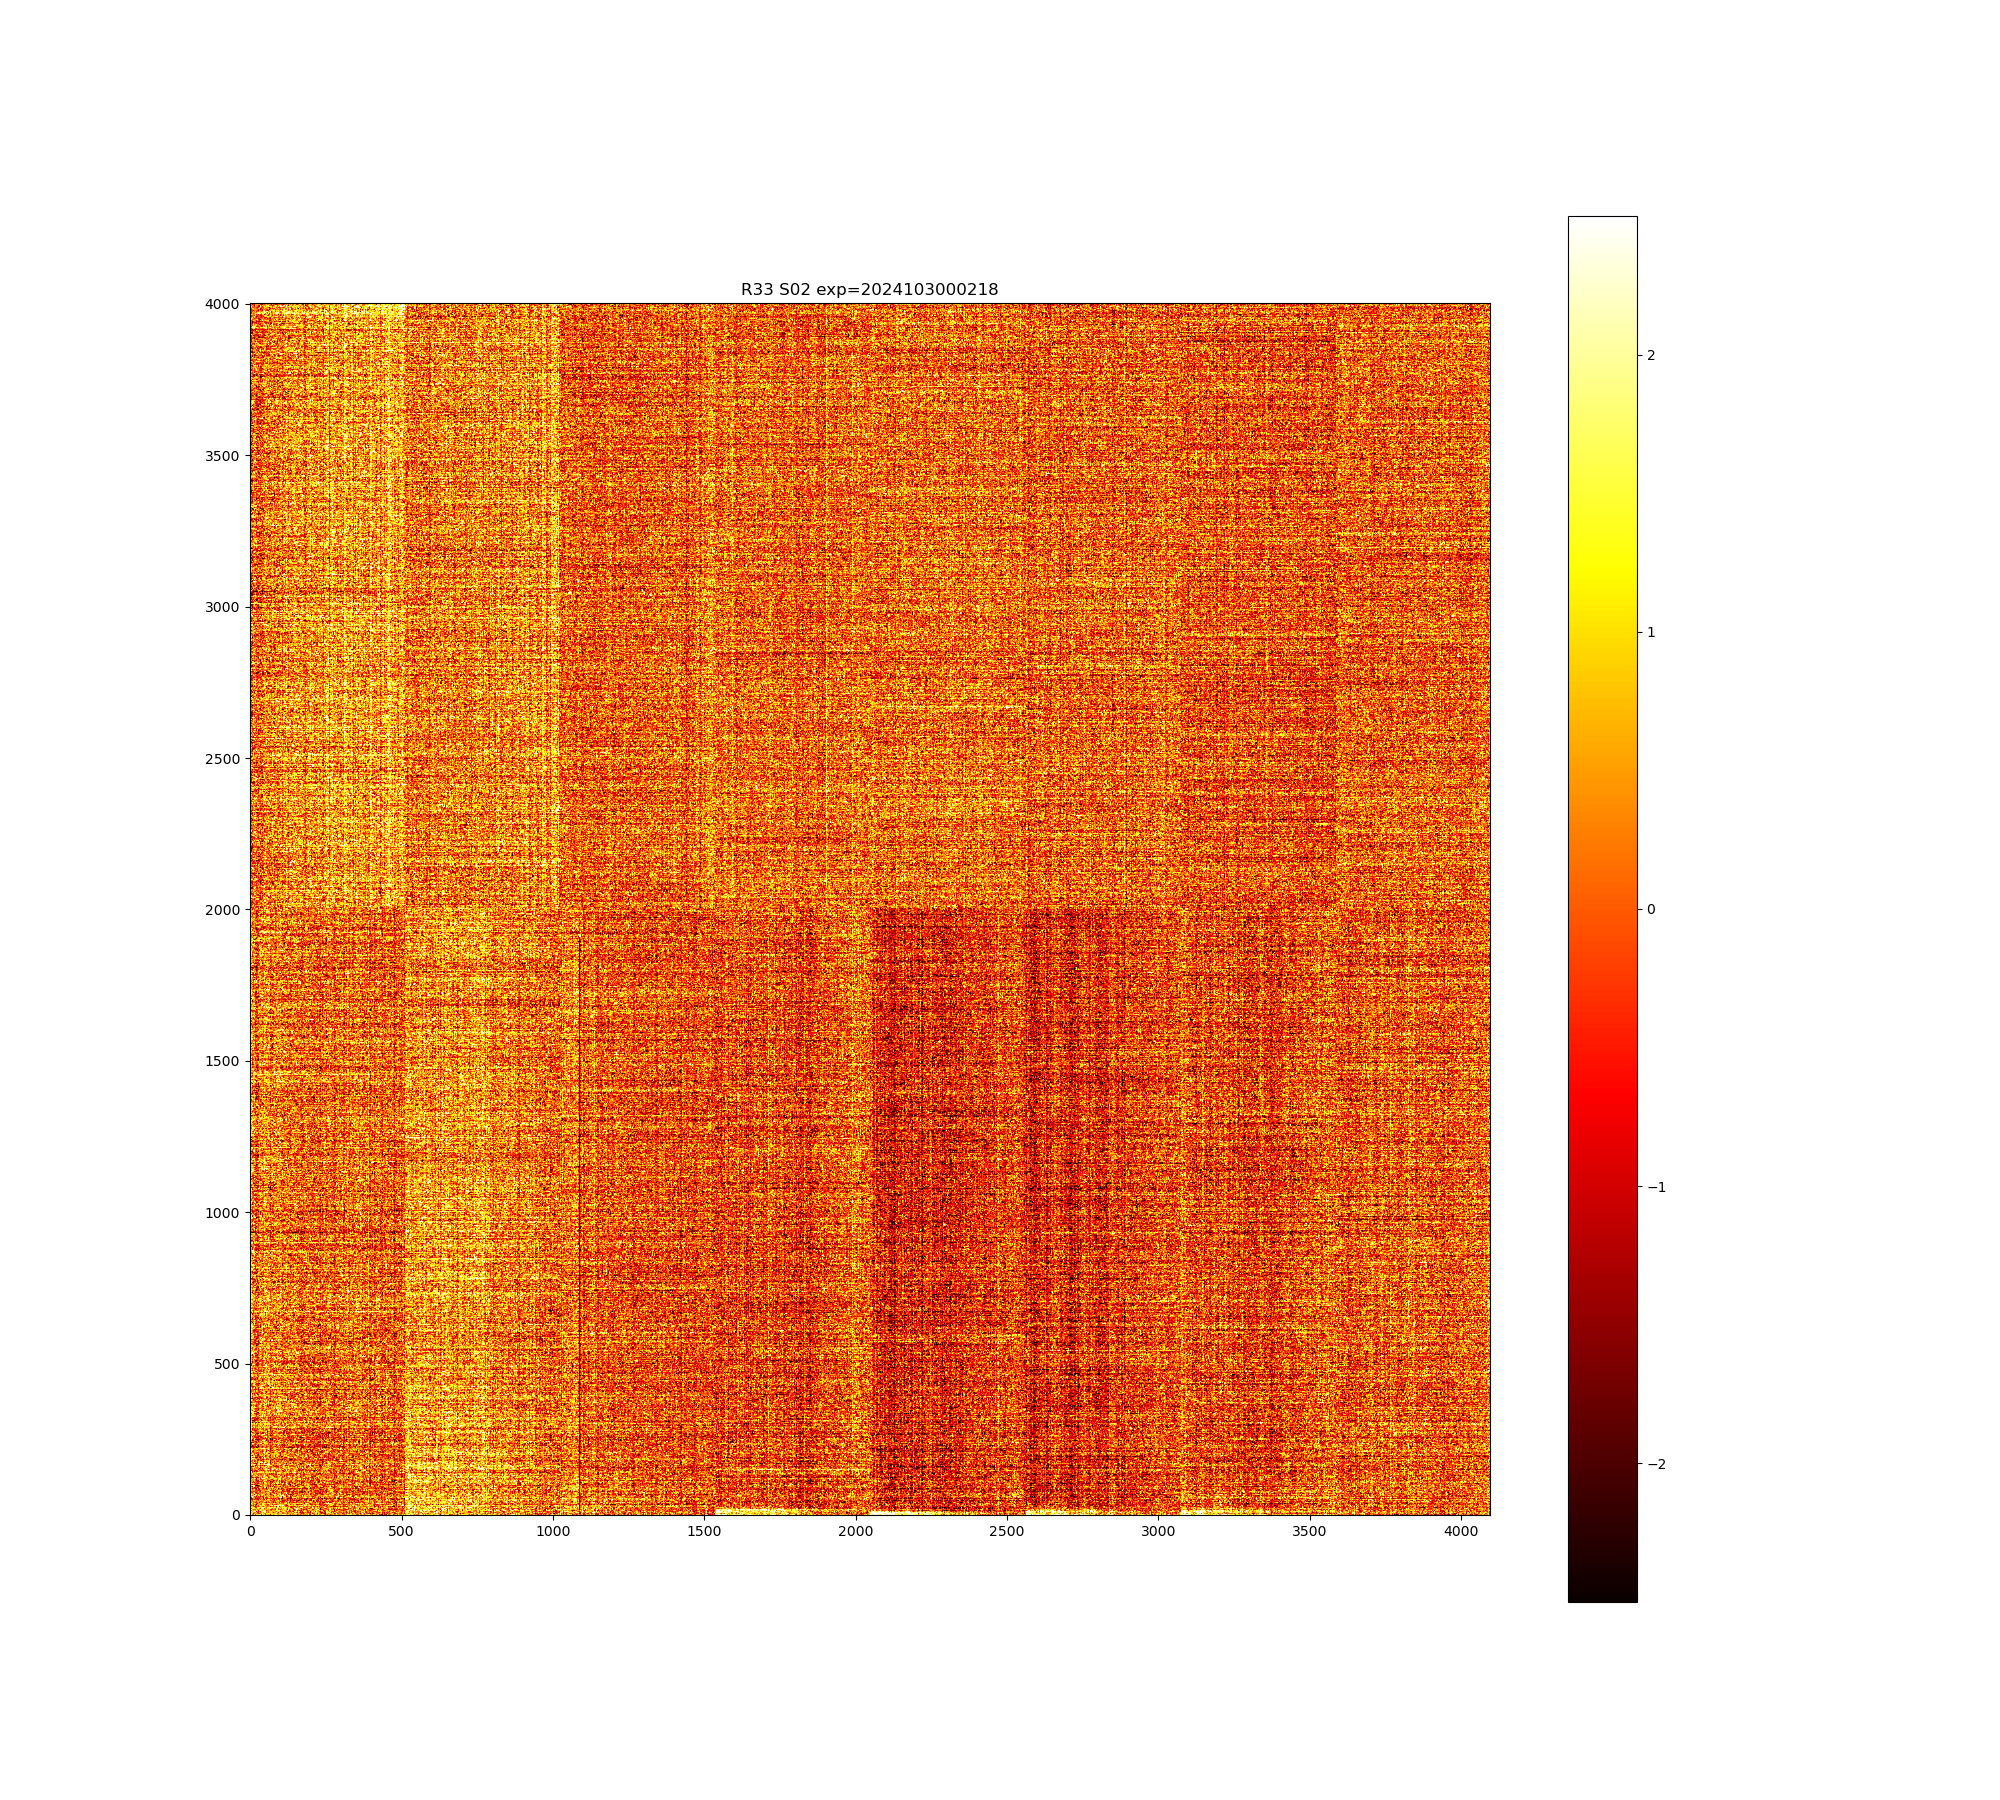
\includegraphics[width=\textwidth]{figures/E1880_bias_R33_S02.png}
    \caption{Bias exposure, run E1880, R33\_S02}
    \label{fig:r33_s02_1880}
\end{minipage}
\hfill
\begin{minipage}{0.45\textwidth}
    \centering
    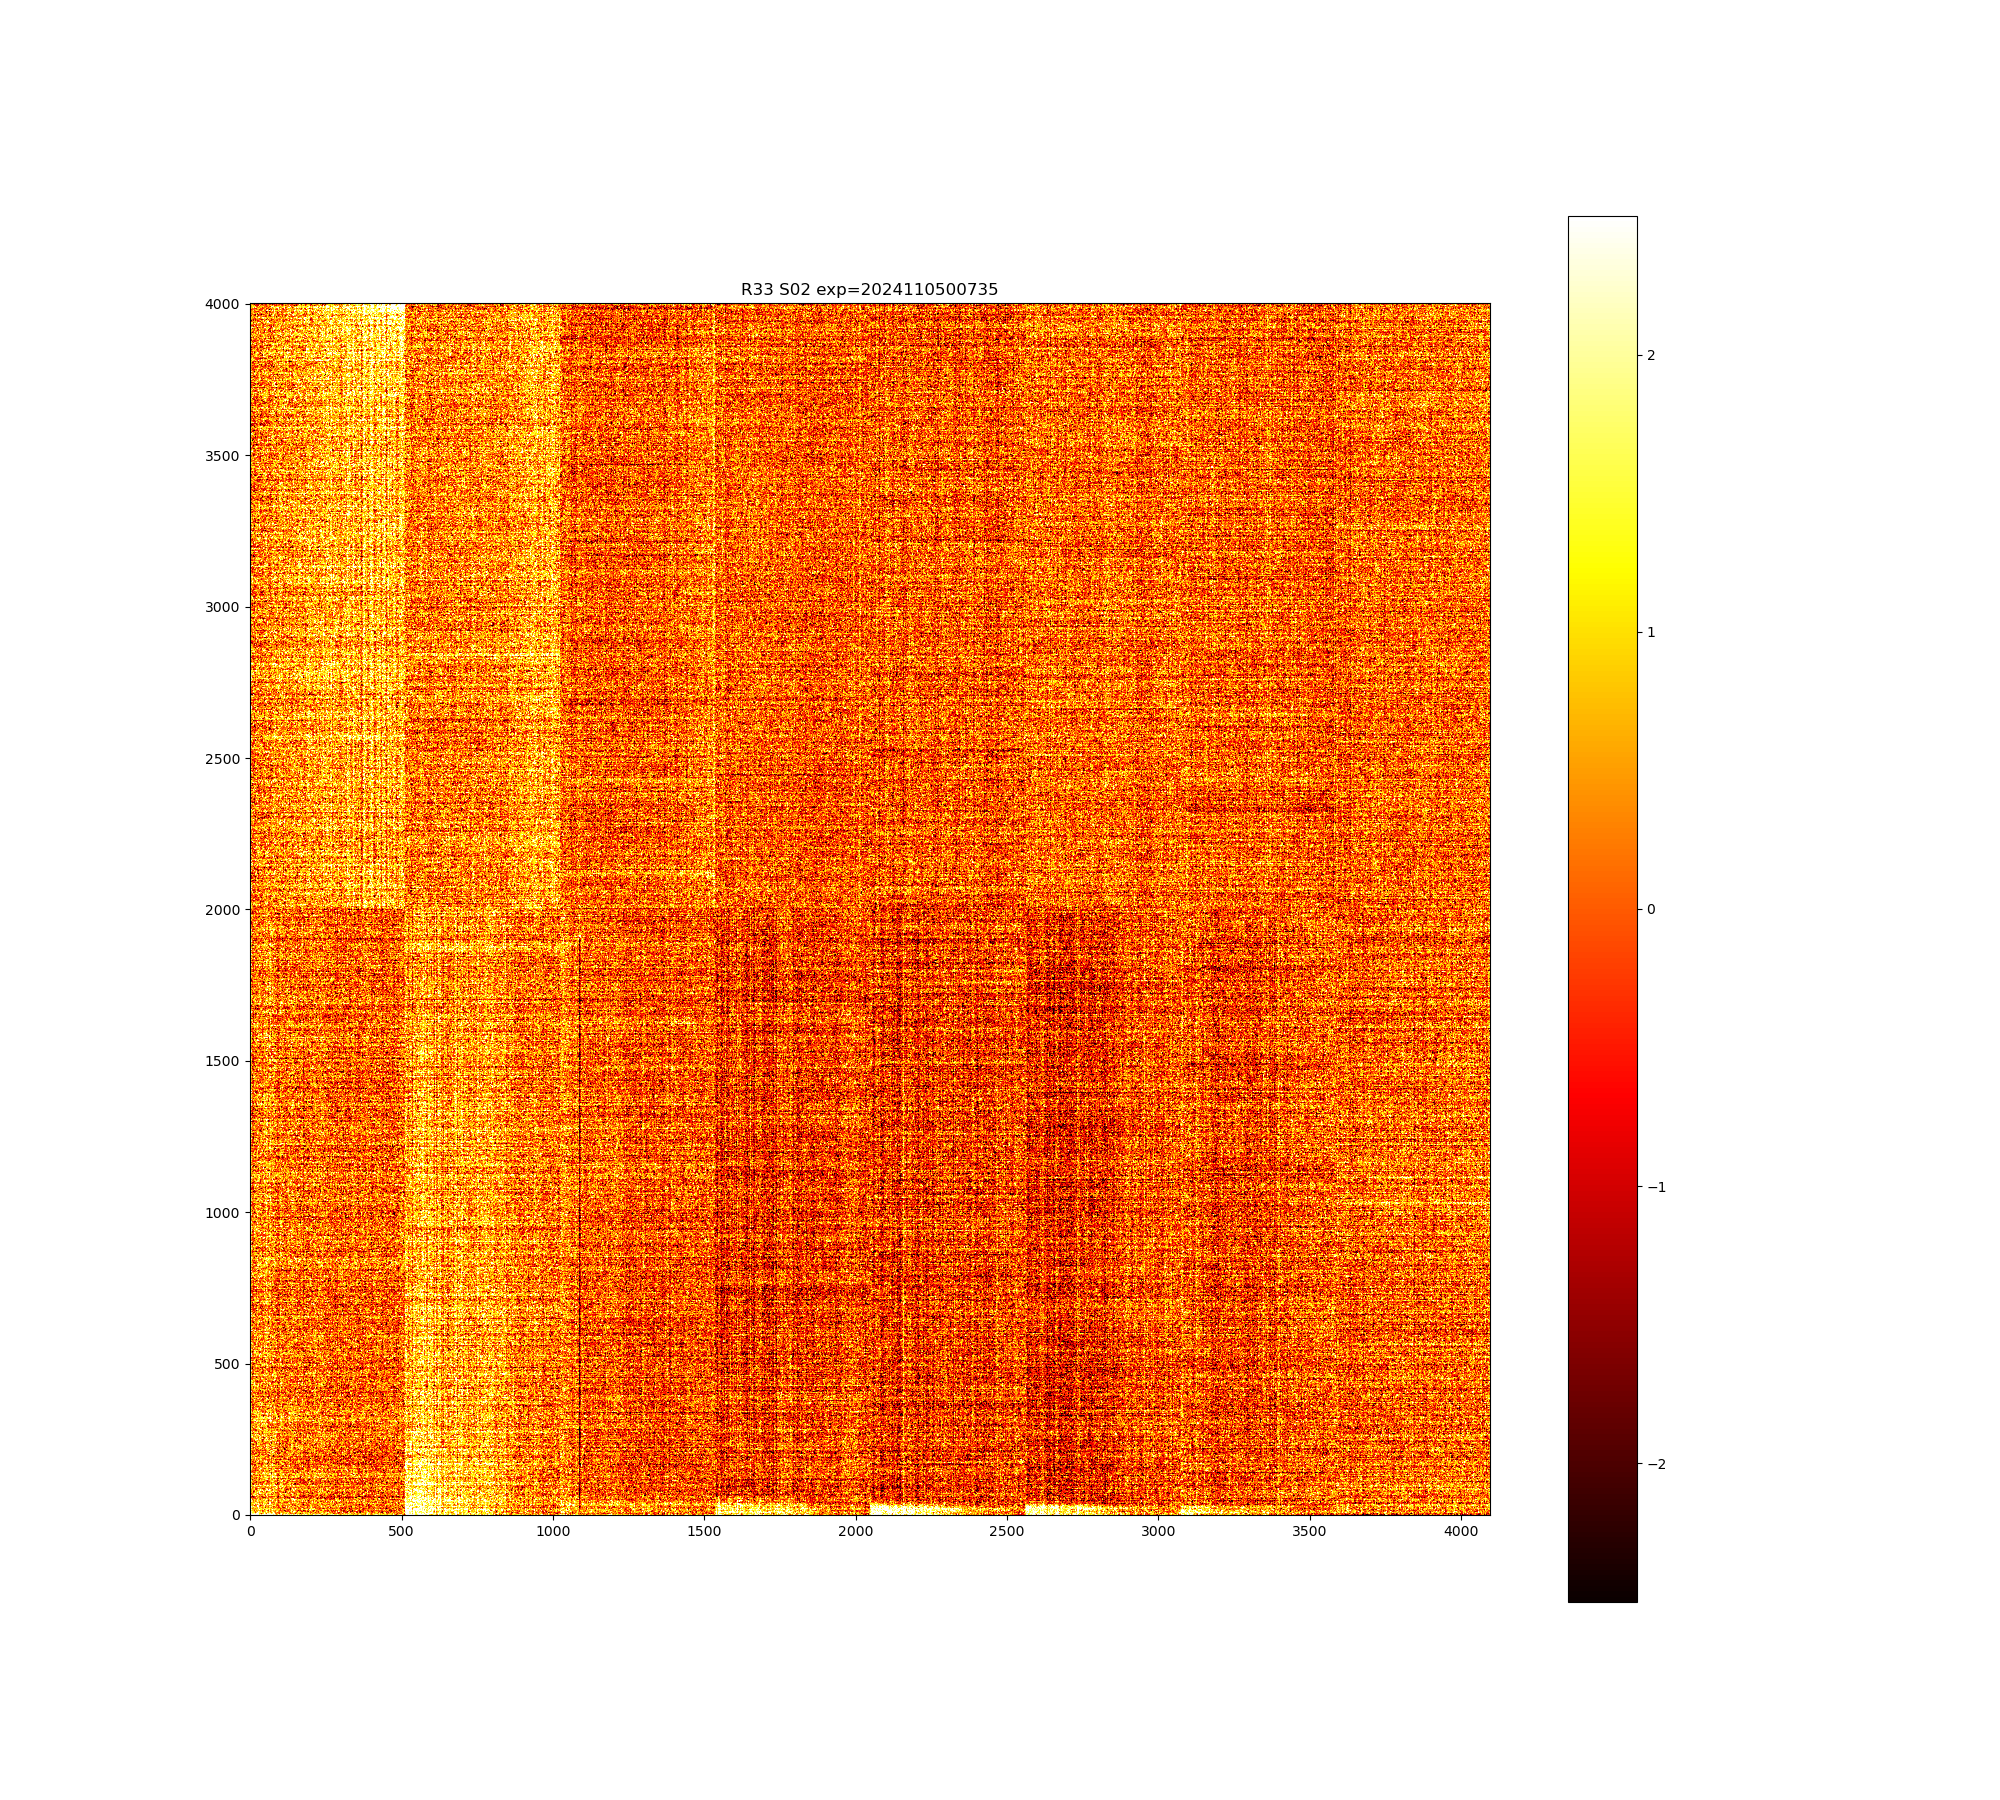
\includegraphics[width=\textwidth]{figures/E2136_dark15_R33_S02.png}
    \caption{15\,s dark exposure, run E2136 in 'stable' conditions, R33\_S02}
    \label{fig:r33_s02_2136}
\end{minipage}

\vspace{0.5cm}

\begin{minipage}{0.45\textwidth}
    \centering
    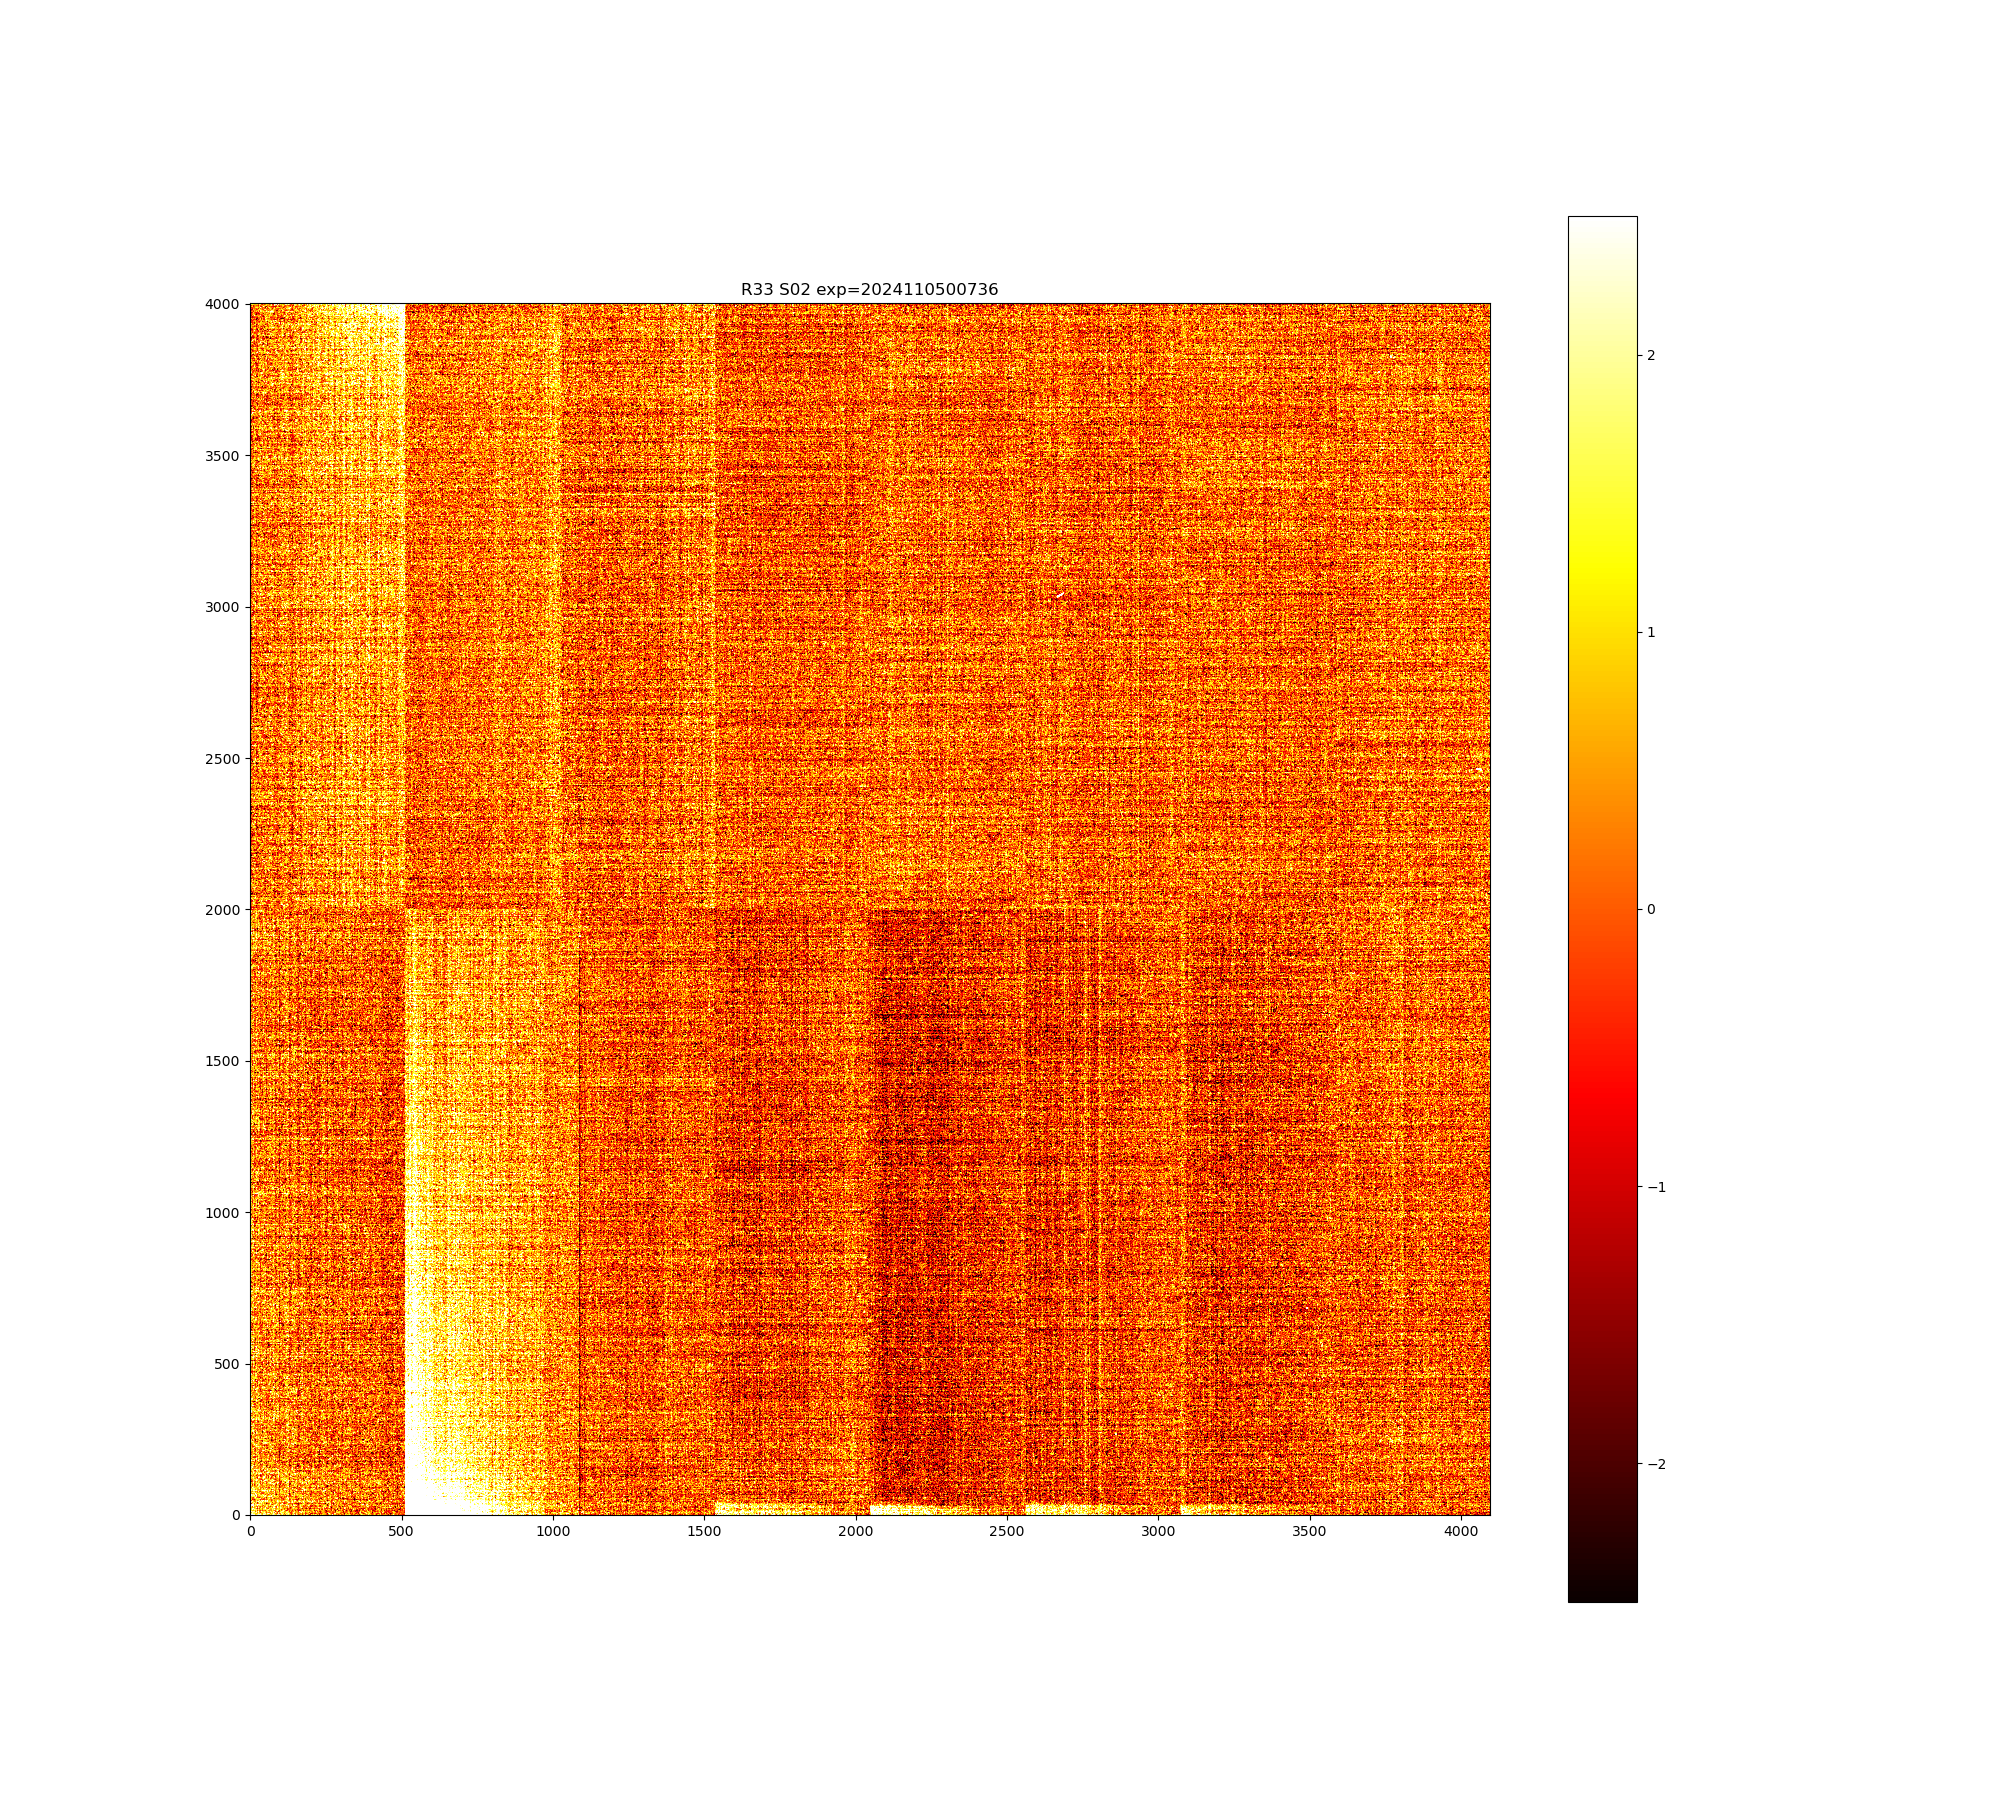
\includegraphics[width=\textwidth]{figures/E2136_dark15_delay_R33_S02.png}
    \caption{15\,s dark exposure, run E2136 after a 3\,min delay, R33\_S02}
    \label{fig:r33_s02_2136_delay}
\end{minipage}
\hfill
\begin{minipage}{0.45\textwidth}
    \centering
\end{minipage}
\end{figure}

In order to quantify the number of unstable e2v amplifiers, a stability
metric \emph{d} is defined from the {\tt eo\_pipe}
stability task data products. More precisely, \emph{d} is defined, for a
given amplifier in a given run, as the difference between the 5th and
95th percentiles of the image mean over all the bias image acquisitions. The
distribution of \emph{d} for run E2136 is shown in Figure~\ref{fig:stability_dist}. Applying a
threshold at 0.3\,ADU (which corresponds to approximately 3 times the value for very stable amplifiers), 51 amplifiers are identified as unstable (see the
corresponding mosaic in Figure~\ref{fig:stability_mosaic}). This corresponds to \sim3\% of the e2v
amplifiers.

\begin{figure}[htbp]
\centering
\begin{minipage}{0.45\textwidth}
    \centering
    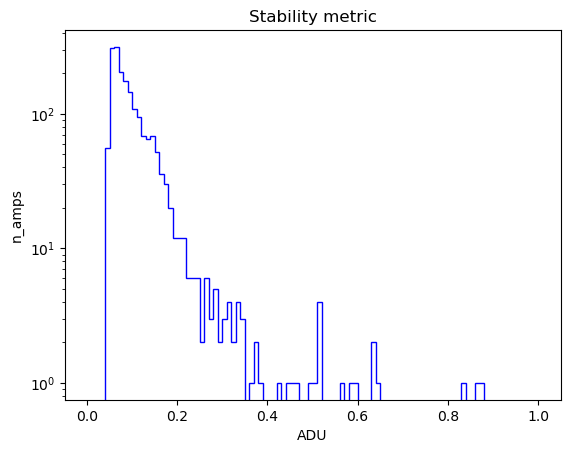
\includegraphics[width=\textwidth]{figures/E2136_distribution_d.png}
    \caption{Distribution of the stability metric for the e2v amplifiers in run E2136}
    \label{fig:stability_dist}
\end{minipage}
\hfill
\begin{minipage}{0.45\textwidth}
    \centering
    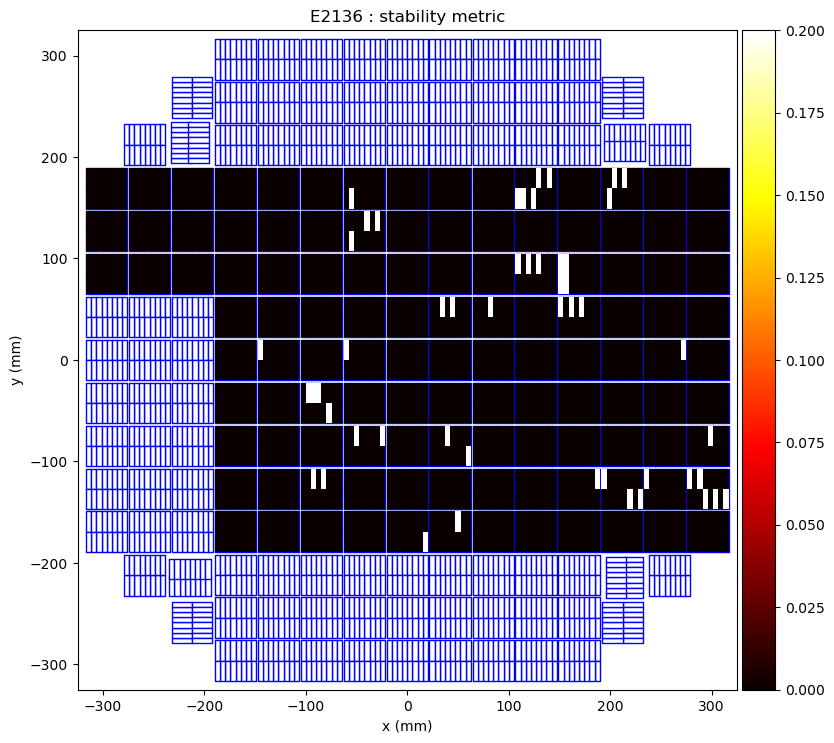
\includegraphics[width=\textwidth]{figures/E2136_mosaic_d.png}
    \caption{Mosaic of e2v amplifiers identified as unstable (white color) in run E2136}
    \label{fig:stability_mosaic}
\end{minipage}
\end{figure}

\clearpage
\subsection{Glow search}
A long dark image can be used to identify glowing regions. Figure \ref{fig:glowsearch} shows an example of a 900\,s dark after ISR application, with a very narrow stretch from -6 to -6 ADUs.
Obvious glow can be found in 3 guider sensors of S04\_SG0, S40\_SG1 and S44\_SG0 (see Fig.~\ref{fig:focal-plane-layout} to locate each sensor). The glows in the guider sensors have been identified and present since their first testing after the Raft construction.
Glowing regions can be observed in R12\_S22, R14\_S22, R23\_S11, as well, along with some other minor glowing regions elsewhere. These are the so-called yellow corner, which we discussed in Section \ref{sec:bias-stability-2}.
In R43\_S21 between Segments 13 and 14, we found a very weak glow at a rate of 40--50\,ADU/900\,s (Fig. \ref{fig:glowsearch:closeup}). This was also present in Run 6 data (e.g., in MC\_C\_20231102\_000085).
Otherwise, we did not find any other glowing regions in the focal plane.

\begin{figure}
    \centering
    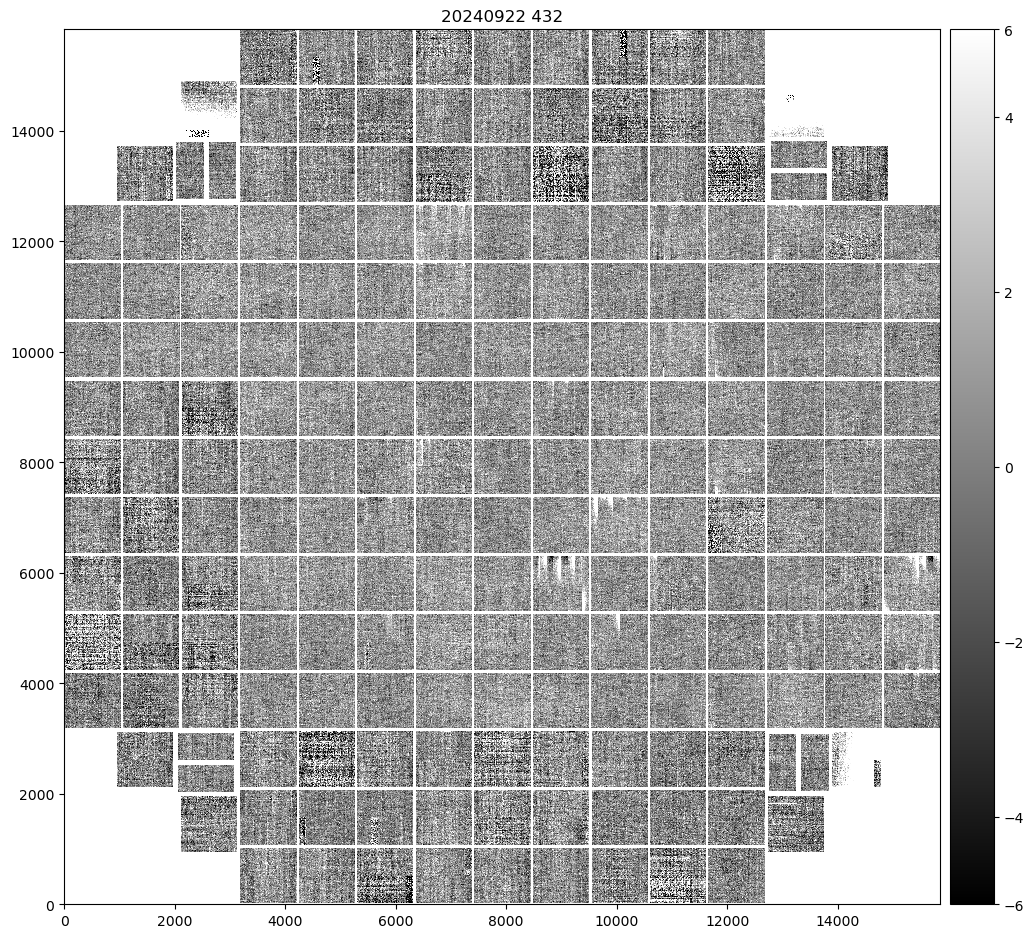
\includegraphics[width=0.5\linewidth]{figures/glowsearch/900sdark.png}
    \caption{A 900\, s dark image MC\_C\_20240922\_000432, after the ISR application.}
    \label{fig:glowsearch}
\end{figure}
\begin{figure}
    \centering
    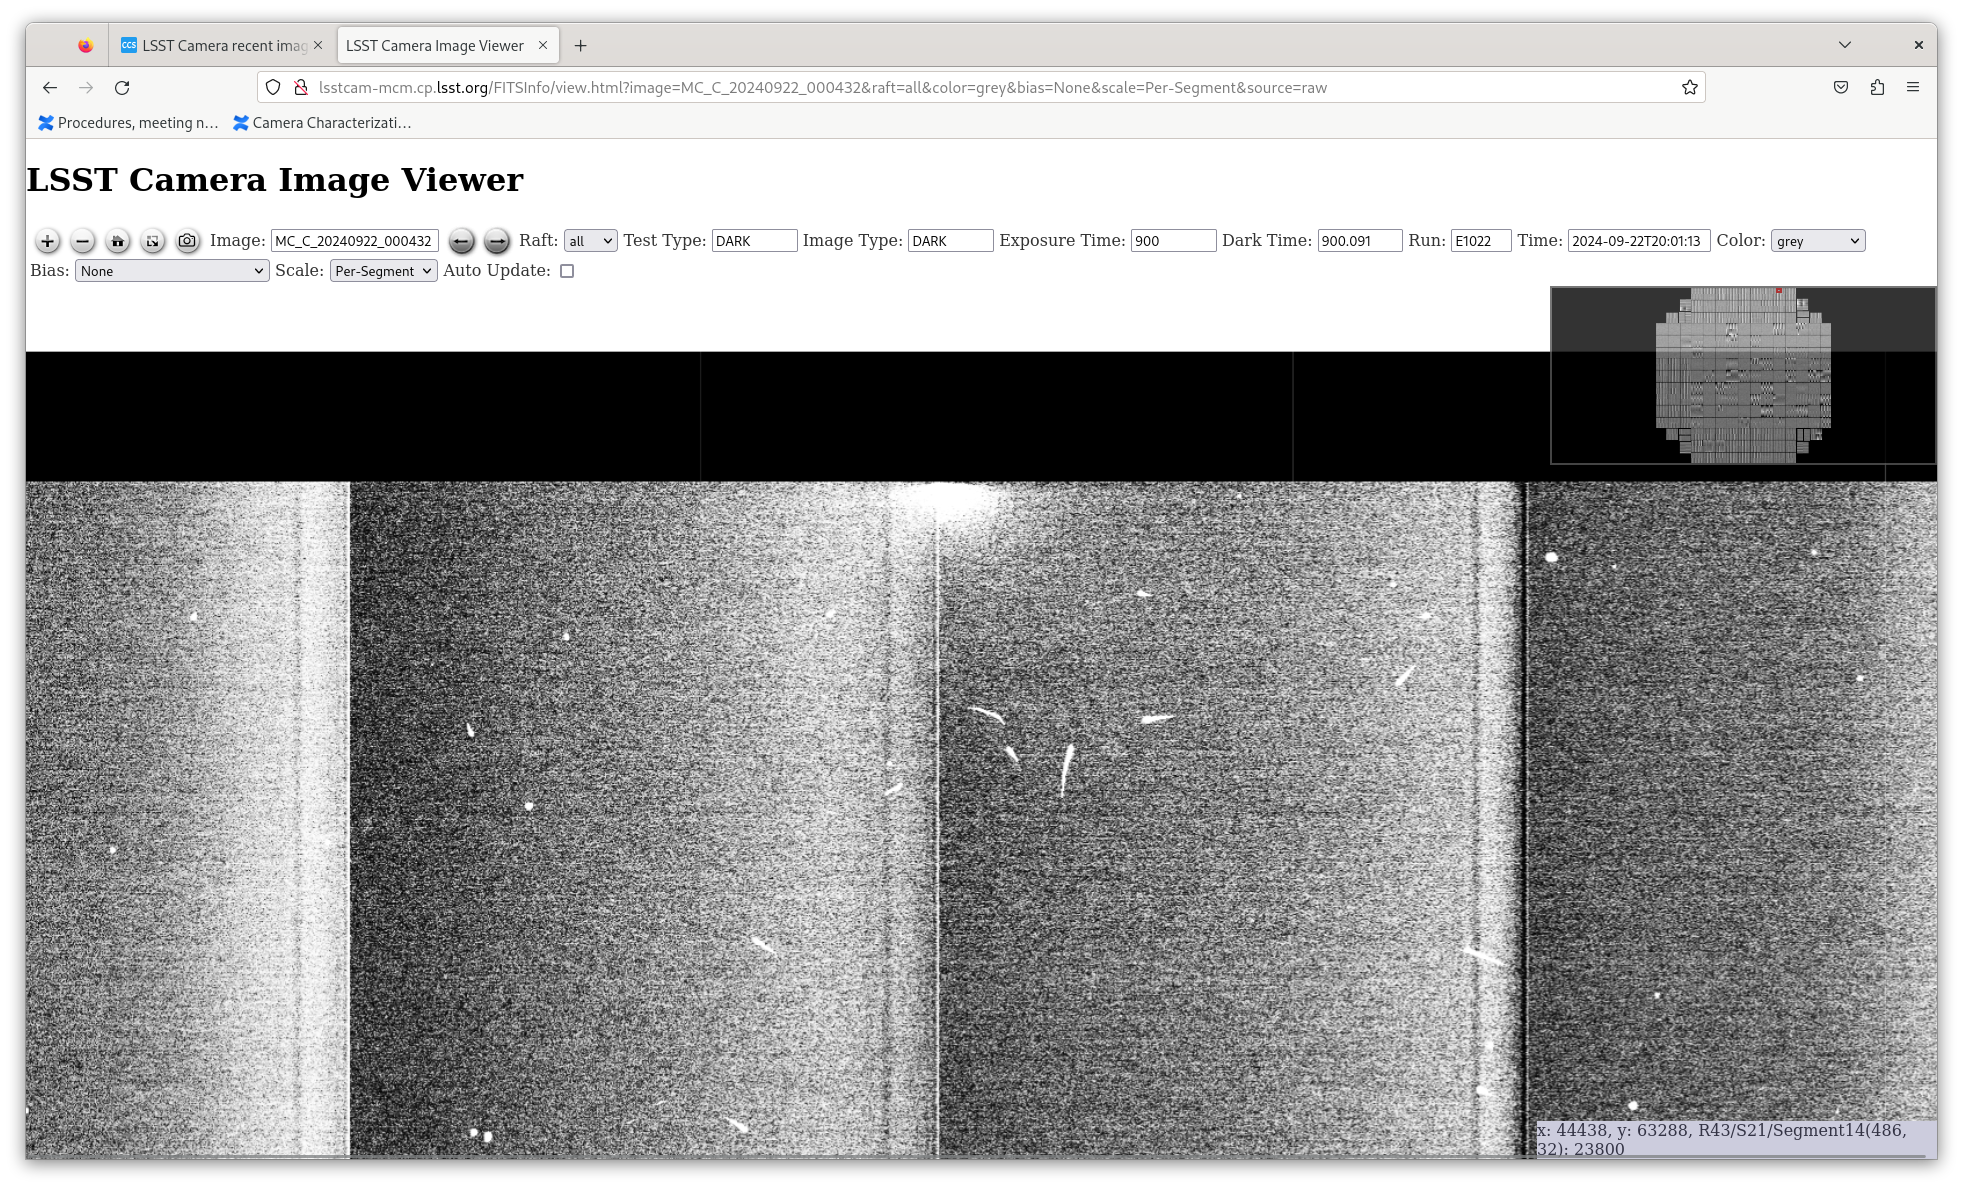
\includegraphics[width=1.0\linewidth]{figures/glowsearch/R43S21.png}
    \caption{A close up of R43\_S21 of a 900\,s dark image MC\_C\_20240922\_000432}
    \label{fig:glowsearch:closeup}
\end{figure}

\clearpage
\subsection{Illumination-corrected flat}

To assess the quality of gain matching over each CCD as well as to study relative QE, we fit the CCOB-wide illumination to a smooth model and plotted mosaics of the full focal plane corrected by the illumination model. The illumination pattern is optimally fit using the 750\,nm LED, since the QE is identical between the e2v and ITL CCDs at this wavelength. To capture the spatial variation of the illumination we fit the response of the focal plane using a {\it lambda} flat image with {\it physical\_filter = 'nm750'} from B protocol run E2233, using cp\_pipe processing with the latest ISRTask\footnote{See \url{https://s3df.slac.stanford.edu/data/rubin/lsstcam/E2233/w_2025_02/}}. PTC gains and linearity corrections, as determined from this B protocol run, are applied to the image and the resulting {\it postISRCCD} is then down-sampled into 32$\times$32 super-pixels for ease of analysis. We take care to remove super-pixels with values in the bottom 5\% or top 0.03\%, values chosen by eye to remove questionable regions of the mosaic.  We modeled the illumination with a two-dimensional product of Chebyshev polynomials: $ I(x,y) = \sum_{i=0}^{5} \sum_{j=0}^{5} c_{ij} T_i(x) T_j(y)$, and fit the coefficients with the {\it least\_squares} method in {\it scipy.optimize}.  The 750\,nm flat and the model fit are shown in Figure~\ref{fig:mosaic-modelfit}.

\begin{figure}[ht]
    \centering
    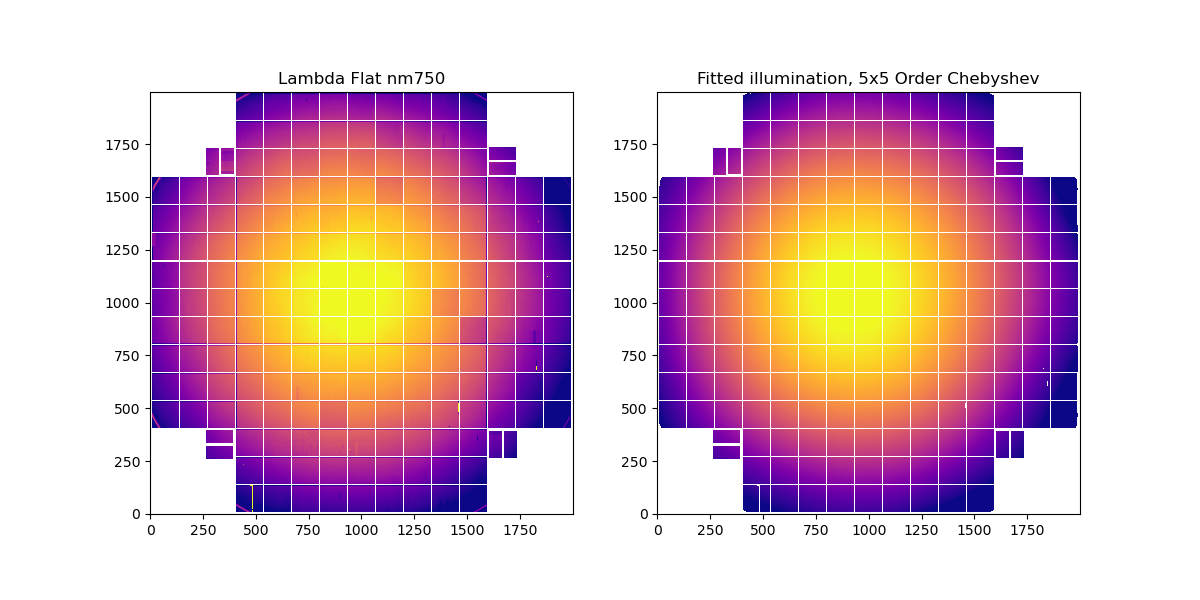
\includegraphics[width=0.95\linewidth]{figures/lambda_nm750_withfit.png}
    \caption{Focal Plane mosaic from a 750\,nm lambda flat (left). Two-dimensional Chebyshev model illumination fit (right)}
    \label{fig:mosaic-modelfit}
\end{figure}

Next, we divide the mosaic images in each CCOB-wide LED by the illumination model fit to produce a relative QE mosaic, as shown in Figure~\ref{fig:mosaic-relativeqe}.  Visually the per-CCD gain matching looks good and we expect to refine this further by using PTC gains and non-linearity from a dense PTC run and by application of  additional ISR pipeline tasks such as CTI, Cross-Talk and bad pixel and column masking to correct these images. We will also compare these mosaics against expectations from the single-raft measured quantum efficiency.

\begin{figure}[ht]
    \centering
    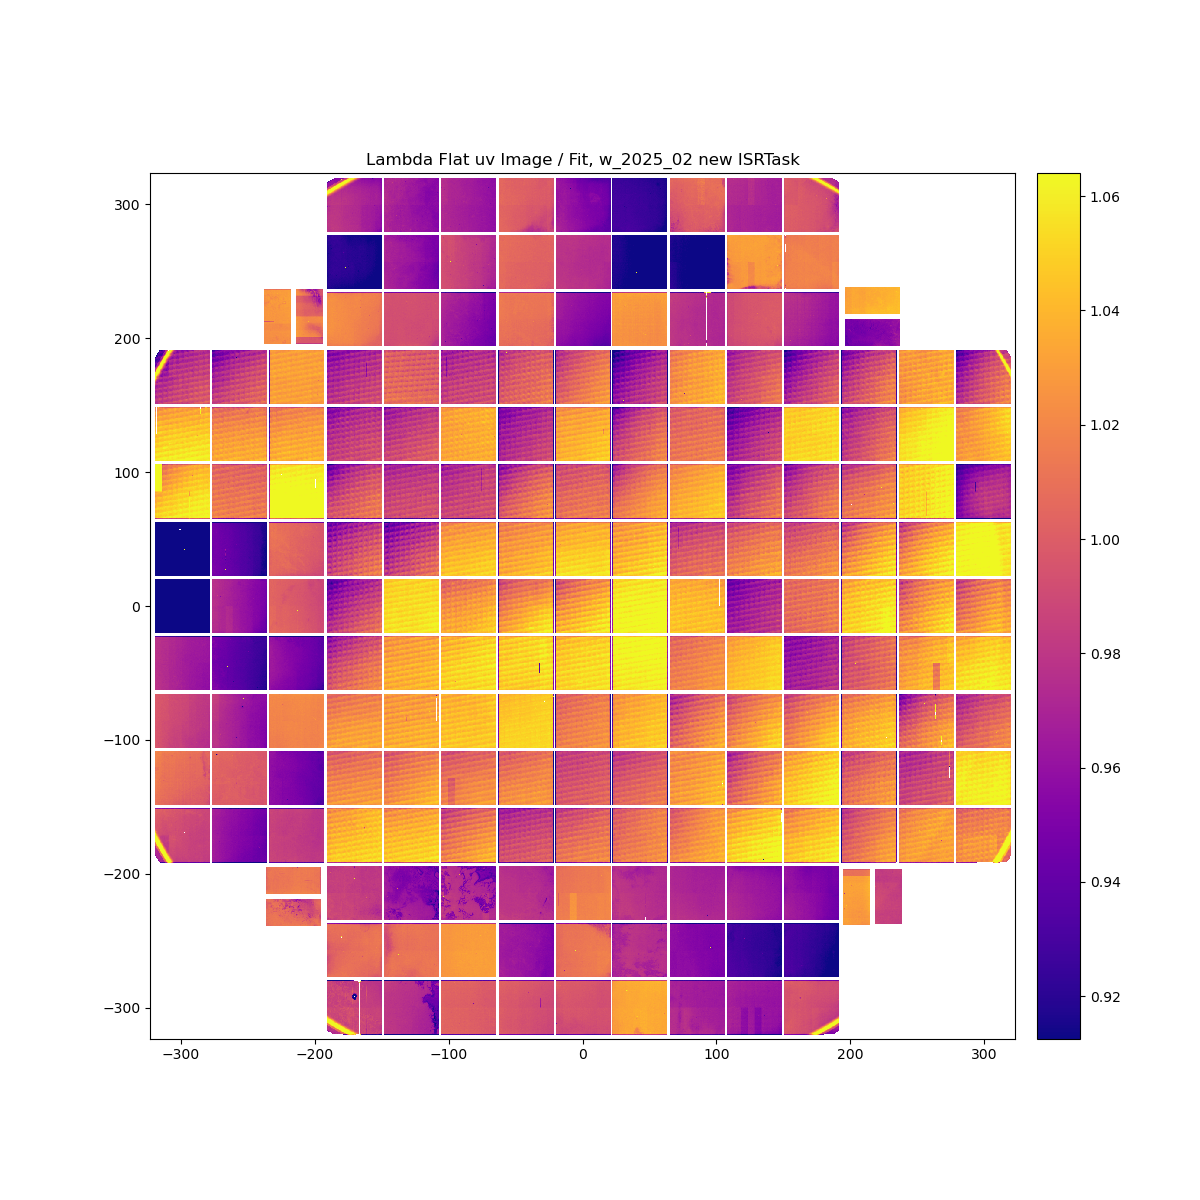
\includegraphics[width=0.4\linewidth]{figures/lambda_uv_E2233.png}
    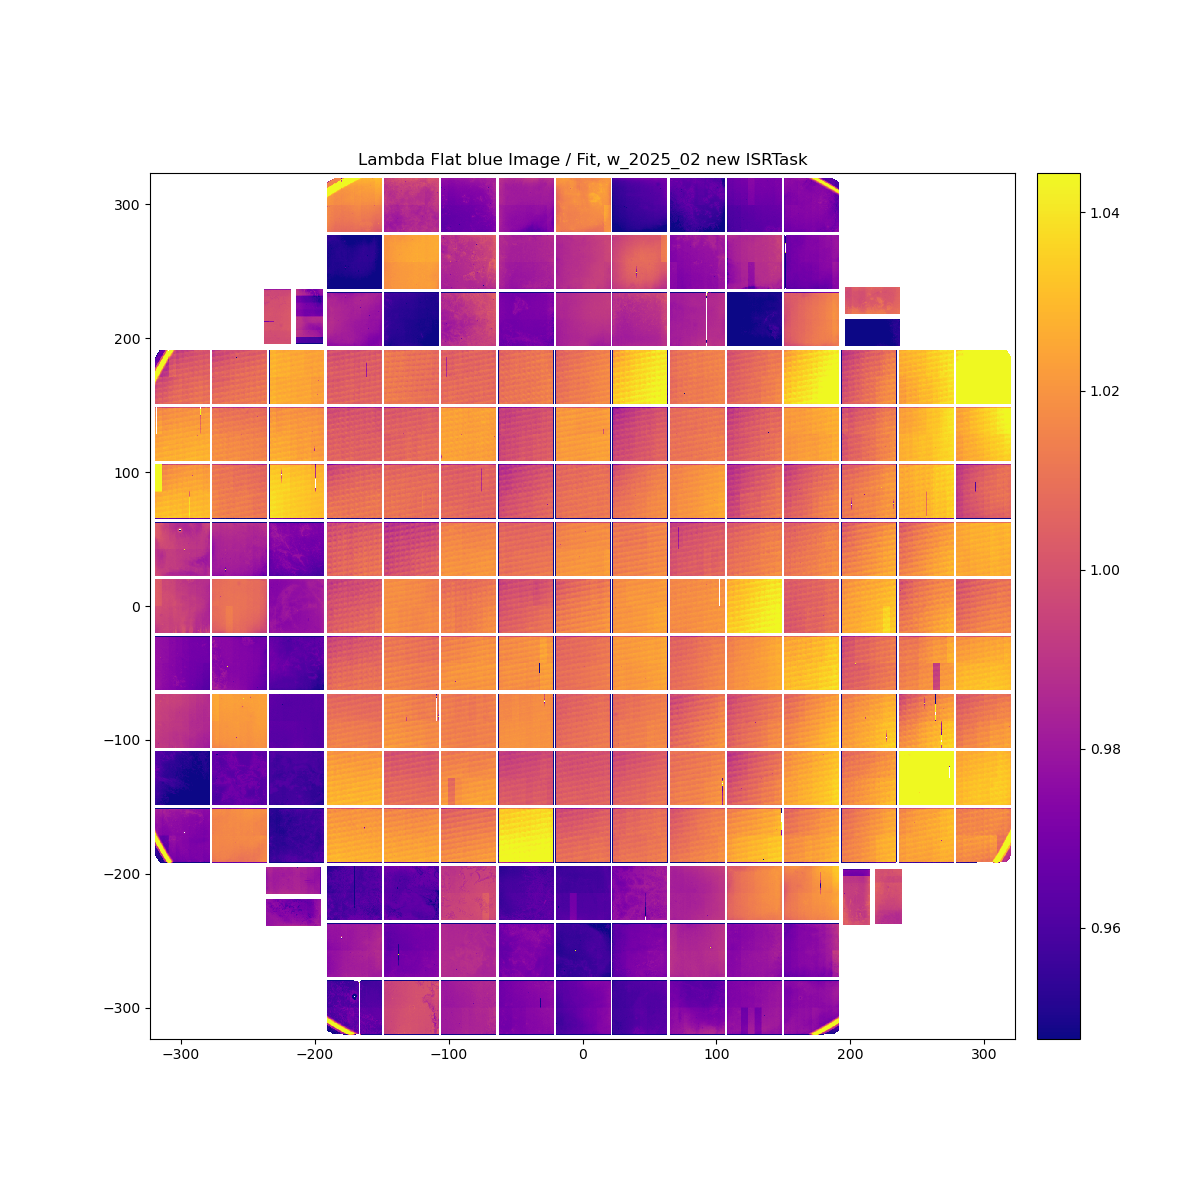
\includegraphics[width=0.4\linewidth]{figures/lambda_blue_E2233.png} \\
    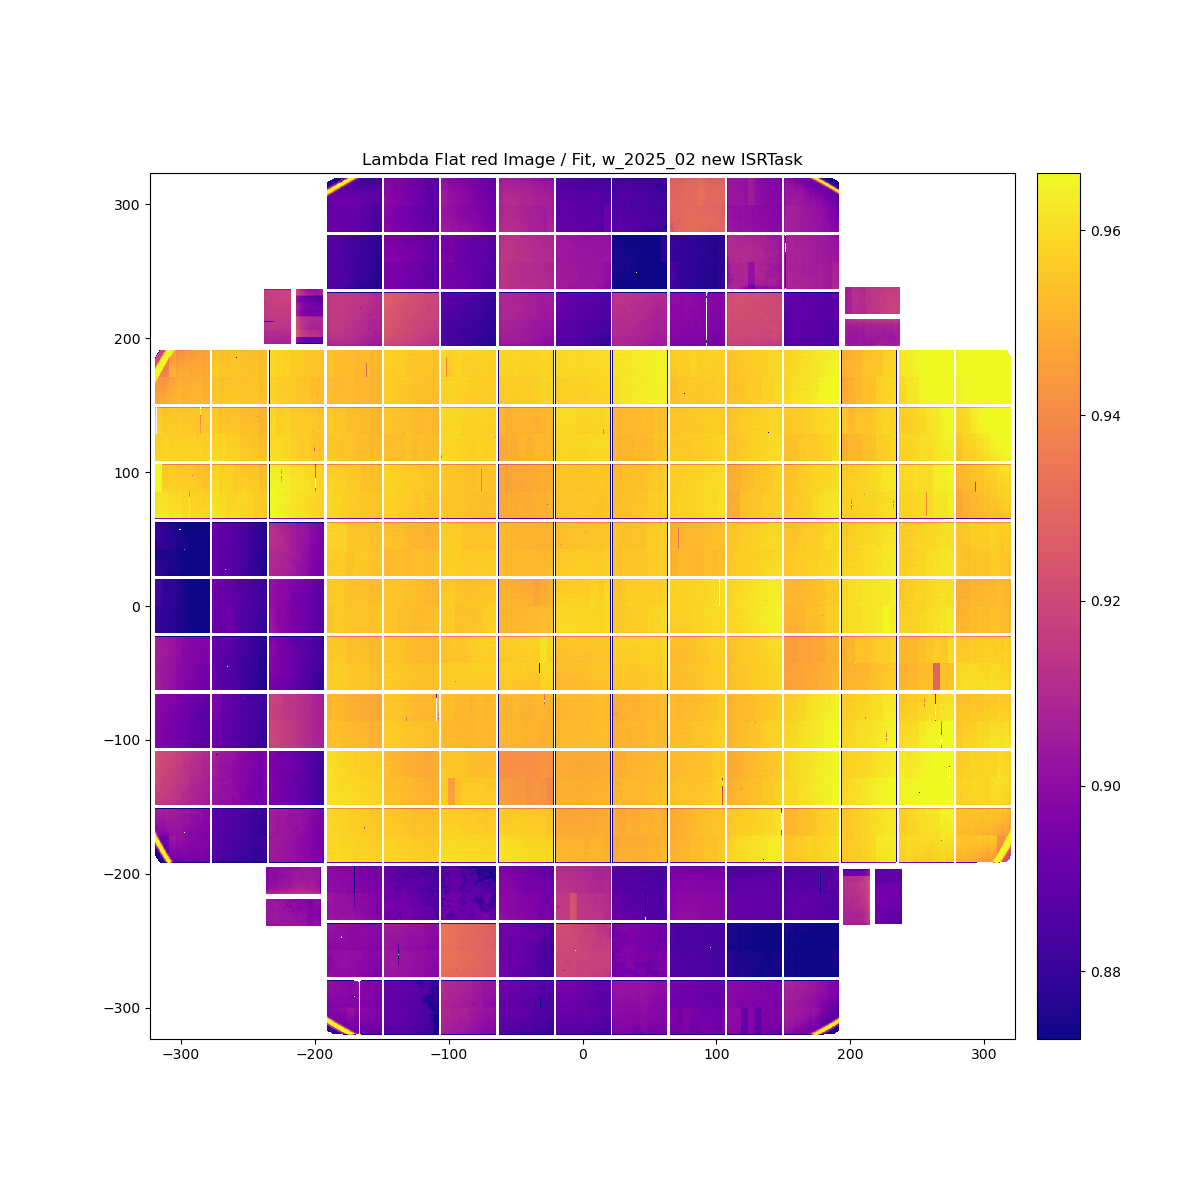
\includegraphics[width=0.4\linewidth]{figures/lambda_red_E2233.png}
    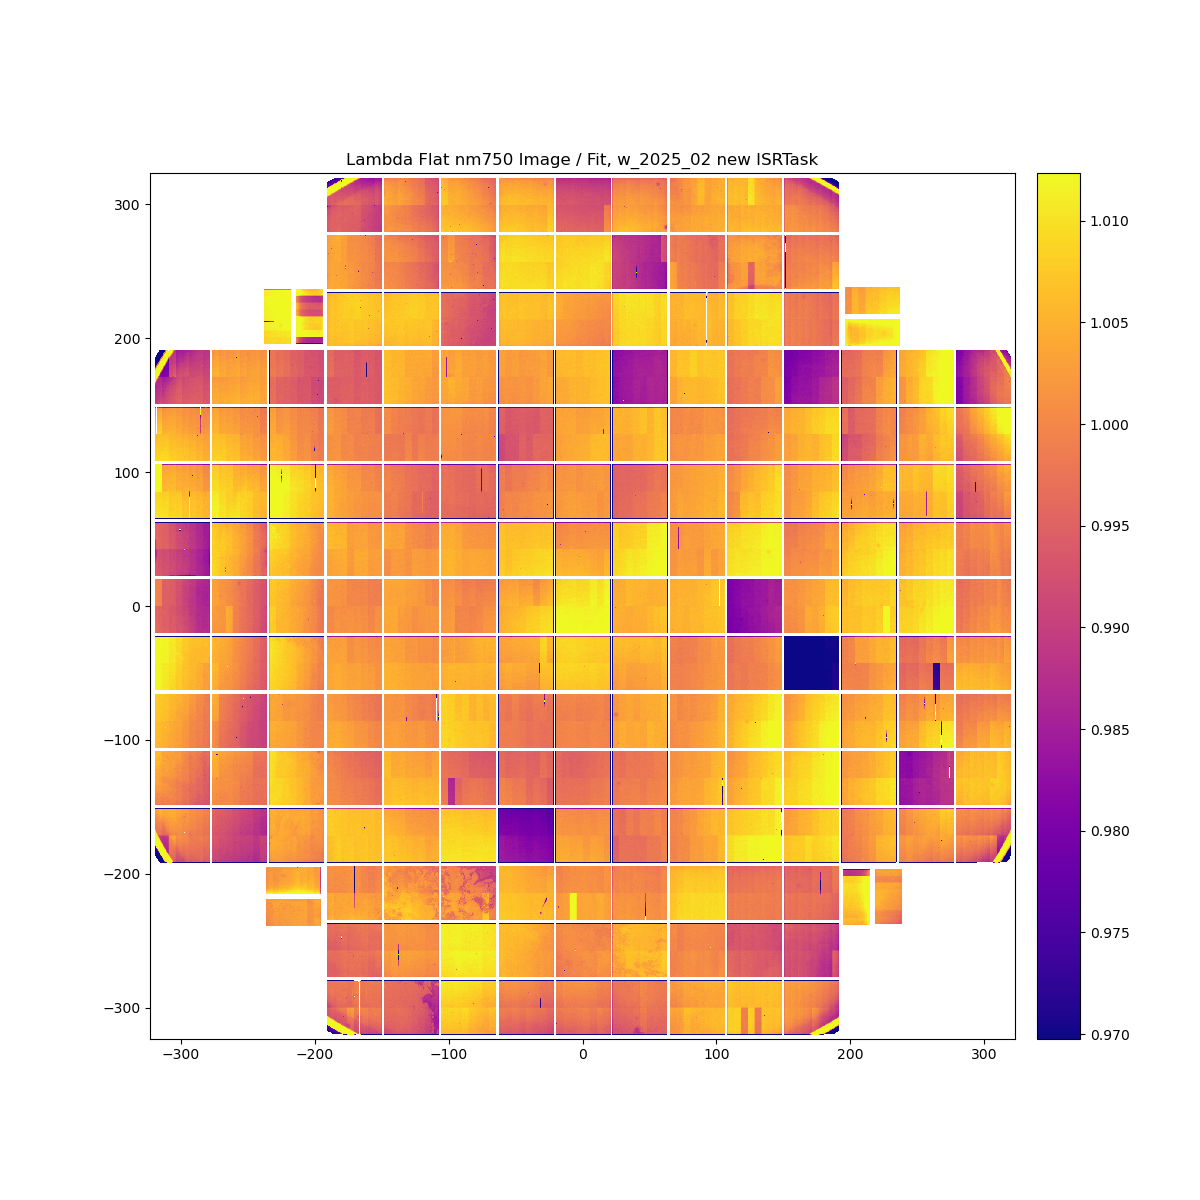
\includegraphics[width=0.4\linewidth]{figures/lambda_nm750_E2233.png} \\
    \includegraphics[width=0.4\linewidth]{figures/lambda_nm850_E2233.png}
    \includegraphics[width=0.4\linewidth]{figures/lambda_nm960_E2233.png} \\
    \caption{Focal plane mosaic for each of the CCOB-wide lambda flats, divided by the corresponding illumination model.}
    \label{fig:mosaic-relativeqe}
\end{figure}

\clearpage

\clearpage
\subsection{Full well measurements}\label{sec:bfullwellmeasurement}

One of the goals of Run 7 was to provide two initial metrics that could be used to determine what pixel value to set the SAT and SUSPECT pixel masks for on-sky data. These pixel masks flag saturated pixels (SAT) and those with levels great enough to be subject to non-linear effects (e.g., brighter-fatter effect) and need further inspection before being used (SUSPECT). For each amplifier, three values were considered: the maximum value recorded for a saturated detection, the PTC turnoff level, and the linearity turnoff (see Sec. \ref{linearity-and-ptc-turnoff} for the definitions used for the linearity and PTC turnoffs). Currently, the SUSPECT pixel mask is set by the PTC turnoff and the SAT pixel mask is set by the linearity turnoff. However, these were determined by flat illuminated images and during Run 6, we found that these values do not match what is found in saturated pinhole images (saturated pinhole values being higher (lower) than the recorded maximum values for e2v (ITL) detectors).

As such, we decided to determine the full well levels using spot images and to compare them to those found with the flat illumination setup. The spots were made using the spot projector and are the circular spots as described in Section~\ref{projector-spots}. For these analyses, we took pairs of images ranging from exposure times of 1--100\,s in 1\,s intervals. To measure a spot, we applied a very loose threshold ($1\sigma$ above the background) to return the footprint and when evaluating the centroid of the spot.

Once we found a spot and its centroid, we evaluated three different turnoff levels: spot photometry, spot PTC, and spot shape.
For spot photometry, we used the spot centroid to place a 5\,pixel\footnote{We plotted the effect of changing the pixel aperture and found that the final turnoff value increases with aperture size. This is because this method is a proxy for measuring when the spot begins to bleed and when the bleeding exceeded the aperture size. As such, we decided to keep it small at 5 pixels.} aperture around the spot. We then plotted the aperture flux divided by the exposure time as a function of the measured peak of the spot as shown in Figure~\ref{fig:Spot_Metrics}. This resulted in an almost constant value until a sudden drop in the flux rate. As such, our metric for the turnoff is when the ratio first starts dropping, whenever the constant value drops below $3\sigma$ of its scatter. This turnoff is shown in Figure\,\ref{fig:Spot_Metrics} as the black line.

For the spot PTC, we utilized the pair of images taken at each exposure level and again using the spot centroid, we selected a 10$\times$10 pixel box around the core of the spot to use for our PTC. We then compared these 10$\times$10 pixel cutouts between the two pairs, finding the average and the standard deviation of the sum of the two boxes. To find the turnoff level, we evaluated the derivative of the variance vs. spot mean and found the point that has the first large negative value (-2000 ADU/s/ADU). This curve and the turnoff are shown in Figure~\ref{fig:Spot_Metrics}.

Lastly, we used the final full well measurement to evaluate the spot shape and its second moments. Instead of using just the centroid from the spot footprint, we utilized the corresponding bounding box to cut out the entire spot. We then ran \texttt{galsim.hsm.FindAdaptiveMom} on the image to measure the value $e_1$\footnote{$e_2$ is also measured but we found that $e1$ had more sensitive measurements, mostly likely due to it only measuring the differences in the spot shape in the X and Y directions while $e2$ measures the difference in the 45 degree direction.}. We then plotted this against the spot peak. Similarly to the spot photometry method, we were left with a constant value that drops off suddenly. We used an approach similar to that for the spot photometry measurements by finding the value that falls below $3\sigma$ of the constant value. The results from applying this method as well as the turnoff values are shown in Figure~\ref{fig:Spot_Metrics}.

\begin{figure}[ht]
    \centering
    \includegraphics[width=0.30\linewidth]{figures/Spot_Photometry.png}
    \includegraphics[width=0.30\linewidth]{figures/Spot_PTC.png}
    \includegraphics[width=0.30\linewidth]{figures/Spot_2ndMoment.png}
    \caption{Example of the different spot metrics and their corresponding calculated turnoffs as the black vertical line for detector R21\_S21 (88). (Left) Spot photometry, (middle) Spot PTC, and (right) Spot second moments.}
    \label{fig:Spot_Metrics}
\end{figure}

We compare these results from Run 7 to the earlier results for flat images. Figure~\ref{fig:Spot_vs_EO_Metrics} shows an example comparison between the three metrics and the PTC and linearity turnoffs from the flat-illuminated data for one detector, R21\_S21. This shows that all three of these metrics correspond to levels a bit greater than the linearity turnoff, providing support that the linearity turnoff is a good metric for defining the SAT pixel mask plane.

\begin{figure}[ht]
    \centering
    \includegraphics[width=0.95\linewidth]{figures/Spot_EO_Comparison.png}
    \caption{Comparison between the calculated Spot full well metrics and the EO metrics. All the Spot metrics are around the level of the linearity turnoff.}
    \label{fig:Spot_vs_EO_Metrics}
\end{figure}

\subsubsection{Spot photometry model}

While R21\_S21 gives good results for all three of these methods, the other detectors are not so clean, especially the ITLs. This is most likely because this detector is in the center of the focal plane while the ITL sensors are arrayed in the outer parts.
The data for the ITLs is messier and the same assumptions and metrics for determining the cutoffs do not work as well. To overcome this, we started using models for the data. To date, this has only been tested on the spot photometry, whose model takes the shape of
\begin{equation*}
    Flux \ rate=a-\frac{1}{bx+c}
\end{equation*}
where $a$, $b$, and $c$ are constants to be solved with the model via \texttt{scipy.optimize.curvefit} and $x$ is the peak value of the spot in ADU. We then classify the turnoff in two ways: as when the model drops by 0.1\% and also when the second derivative of the model drops below a certain amount (50 ADU/s/ADU$^{2}$). Figure~\ref{fig:Spot_Model} shows an example of the data, corresponding model, and the two turnoffs.

\begin{figure}[ht]
    \centering
    \includegraphics[width=0.95\linewidth]{figures/Spot_Photometry_Model.png}
    \caption{Example of applying a model to the data for turnoff determination with an ITL detector (R42\_S20). The data is shown in blue, the model in orange and the two turnoff determinations in red and black.}
    \label{fig:Spot_Model}
\end{figure}

This also needs some tuning but should be less susceptible to changes across the focal plane (i.e., noisier data and different spot light levels). The work to apply this method to the whole focal plane is still on-going.
% Figure XXX then compares this with the linearity turnoff for the whole focal plane.

\clearpage
\subsection{Non-linearity studies}\label{nonlinearity}


PTC runs are meant primarily to measure variance and co-variance curves. We collect pairs of flat images, obtained using the CCOB wide-beam described in Section~\ref{sec:electro-optical-setup}. To cover the entire dynamic range of the CCDs, we vary the length of the LED flash, the number of flashes, and the current of the LED. These data sets can be used to measure nonlinearity by comparing the CCD response to the integrated signal measured from a photodiode installed on a port of the integrating sphere that feeds a picoammeter. To avoid any shortcomings from picoammeter nonlinearity, we only compare photodiode signals of the same amplitude (illumination intensity) but different durations. We do not assume that integrated charges measured at different LED currents (and hence different photodiode currents) are on the same scale, although this turns out to be essentially true, as discussed later.

For the nonlinearity study, we use the average signal measured on each CCD channel separately, using 2D overscan subtraction and masking outlier pixels. The photodiode signal is simply bias-subtracted and time-integrated.

Technically, we model the nonlinearity using a spline function that we fit to the CCD/photodiode data pairs by minimizing:
\begin{equation}
Q = \sum_{ij} w_{ij}^2 \left( \frac{ S(\mu_{ij}) +\mu_{ij}  }{D_{ij} f_i} -1 \right)^2
\label{eq:nonlin0}
\end{equation}
where $Q_{ij}$ is the CCD signal measured in exposure $j$ at LED current $i$,
$D_{ij}$ is the corresponding photodiode signal, $f_i$ is the ``photodiode factor" for current $i$, $S$ is the spline nonlinearity correction, and $w_{ij}$ is some weight. We add two constraints: the average of the spline over the fitting range is zero $<S(\mu)=0>$, and $S(0) = 0$. If we choose equal fitting weights $w_{ij}=1$, the residuals exhibit a scatter that varies strongly with signal level, and hence forbid meaningful outlier detection. We model the fitting weights $w_{ij}$ using an expression determined empirically, $w_{ij} = 1/\sqrt{c^2+v^2/\mu_{ij}}$, and the two extra parameters, $c$ and $v$ are also fitted by turning the least-squares expression \ref{eq:nonlin0} into a maximum likelihood one:
\begin{equation}
Q = \sum_{ij} w_{ij}^2 \left( \frac{ S(\mu_{ij}) +\mu_{ij}  }{D_{ij} f_i} -1 \right)^2 - 2 \sum_{ij} \log w_{ij}
\label{eq:nonlin1}
\end{equation}
We fit the spline coefficients, the $f_i$ factors (there are typically 3 of them), and the weight parameters $c$ and $v$, for every image segment separately. We perform an iterative 5$\sigma$ outlier rejection which rejects on average $\sim $0.5\% of the data points (this small rate validates the modeling of weights). Figure~\ref{fig:nonlin_model} displays some results of the fits. The quality of the measured non-linearity is sufficient for our needs.

\begin{figure}[ht]
\begin{centering}
\includegraphics[width=0.9\textwidth]{figures/nonlin_plots.png}
\end{centering}
\caption{top: fitted nonlinearity spline (divided by the signal level) for the 16 channels of R22\_S11. The main feature is due to the distortion introduced by the preamplifier. Left bottom: The fit residuals for channel 0 of the same CCD. Different colors refer to different LED current settings. Bottom right: r.m.s. of high-flux fit residuals (the $c$ parameter of the fitted dispersion model) for all camera channels. Those are about $10^{-4}$ on average, and some are correlated within REBs, for an unknown reason. The quality of the obtained correction is well within goals.\label{fig:nonlin_model}}

\end{figure}

%\subsection{ADC differential nonlinearity}
%ADC differential nonlinearity (DNL) was studied in earlier runs and will be analyzed separately for Run 7.
% Renee this section later using her method based on runs taken during Run 7.


\subsection{Gain stability}\label{sec:gain-stability-2}
We have used ``relative gain'' in this section to study gain stability over time.
The relative gain is defined as the ratio of the signal observed in a CCD image segment divided by the integration of the photodiode current with respect to an arbitrary normalization.
With a fixed flat illumination, the variation of the relative gain over successive exposures can be utilized to investigate the gain stability.
In the past Run 6 \citep{2024SPIE13103E..0WU}, we used a run during which the Cold plate target temperature was kept constant, which reflects the real observing condition. We repeated this test during Run 7 and we acquired flat images at two representative flux levels with two distinct temperature conditions: either intentionally altered or maintained constant.
\begin{itemize}
    \item E1496 (dp80, 12\,hr, constant temperature, v29\_Nop, nm750, 10k e-)
    \item E1367 (dp80, 6\,hr, temperature swing of 2 degrees, v29, nm750, 50k e-)
    \item E756 (dp80, 6\,hr, gain stability @ 50k e-), unprocessed because there was a data transfer issue
    \item E1362 (dp80, 6\,hr, 10k e-), unprocessed because there was data transfer issue
\end{itemize}

Here we focus on E1496 (steady temperature) and E1367 (variable temperature).

\begin{figure}[htbp]
\centering
\begin{minipage}{0.45\textwidth}
    \centering
    \includegraphics[width=\textwidth]{figures/gaintemp/E1496RelgainParametersTrending.png}
    \caption{relative gain changes with other parameters for one amplifier R01\_S00/C11 in run E1496.}
    \label{fig:relgainparamE1496}
\end{minipage}
\hfill
\begin{minipage}{0.45\textwidth}
    \centering
    \includegraphics[width=\textwidth]{figures/gaintemp/E1496RelgainDetail.png}
    \caption{Relative gain as a function of REB temperature (average of TEMP6 and TEMP10), with color based on temperature swing run E1496. The fitted line and the line with the slope taken from Run 6 are also displayed. The intercept of the Run 6 line is arbitrary, since the operating temperature was different.}
    \label{fig:gaintempE1496}
\end{minipage}
\end{figure}
Figure \ref{fig:relgainparamE1496} shows the derived
 relative gain change for one amplifier (R11\_S00\_C11) over time along with other representative parameters such as the average of two REB temperatures measured closest to the ASPICs, (TEMP6+TEMP10)/2, CCD temp, and LED1TEMP (the temperature measured at the LED board on the CCOB projector). In Run 6, the REB temperature average was found to be a good proxy for the relative gain change.
 For the steady temperature acquisitions, the REB temperatures were maintained steady within 0.2\, C, with a slight decreasing trend during the run probably due to the change in the thermal load and the stabilization process of the entire thermal system.
During the run the gain slowly increased over time, while the CCD temperature remained steady and the LED temperature was not controlled but stayed within an 0.1\,C range.

 Figure \ref{fig:gaintempE1496} shows the relationship between the relative gain and the REB temperature, with color coding by the rate of temperature change, along with its fit. A reference line from the past result is overlaid with an arbitrary vertical offset. Clearly, the gain-temperature relationship is steeper than the previous result. The distribution of the data points has a more complicated structure than the linear relationship, while there is no obvious change in either CCD or LED temperatures.



\begin{figure}[htbp]
\centering
\begin{minipage}{0.45\textwidth}
    \centering
    \includegraphics[width=\textwidth]{figures/gaintemp/E1367RelgainParametersTrending.png}
    \caption{Same as Figure \ref{fig:relgainparamE1496} but for run E1367.}
    \label{fig:relgainparamE1367}
\end{minipage}
\hfill
\begin{minipage}{0.45\textwidth}
    \centering
    \includegraphics[width=\textwidth]{figures/gaintemp/E1367RelgainDetail.png}
    \caption{Same as Figure \ref{fig:gaintempE1496} but for Run E1367.}
    \label{fig:gaintempE1367}
\end{minipage}
\end{figure}

Figures \ref{fig:relgainparamE1367} and \ref{fig:gaintempE1367} show the same set of plots but for the run that has a cold plate temperature change of 2\,C.
The temperature was kept steady in the beginning, but the set point was changed later, and then it was brought back to the original temperature.
Clearly, Figure~\ref{fig:gaintempE1367} shows not only temperature dependency but also hysteresis in the gain-temperature relationship, which does not match the slope originally derived from past runs, although there are no obvious changes in the system other than the REB temperature.
During this run the LED board temperature also decreased by more than 1\,C over the testing period.


The reason why the relationship between gain and temperature became much more complicated is not clear. It is understandable that hysteresis was not observed in Run 6 because there was no intentional temperature change in the cold plate, which means the cold plate/REB temperature swing was minimal. However, looking at the result from E1496 where we took images at the same temperature, the relationship is much more complicated than what it looked like before. A number of possibilities can be considered to explain this: 1) there is a hidden variable that changes the gain other than the REB temperature, 2) illumination from the LED is somehow changing over time, which is not correlated with the LED temperature, 3) air turbulence in the lens volume contributes to this, or 4) condensation on the lens might come into play. As hysteresis is observed, possibility 1) is definitely relevant but the particular hidden variable is not clear because it cannot explain the gain changes when the temperature is constant. Possibility 2) is unlikely given the fact that the complicated relationship was observed as well in Run 6. Possibility 3) could play some role since \citet{2024arXiv241113386B} discovered illumination changes due to turbulence of the air in the lens volume. However, it is not clear if any kind of long-term trend over 6 hours can be explained by this. For possibility 4), we made a visual check for condensation (not during the run) and we did not find anything obvious.

Gain changes can be categorized in two ways: global or local to an amplifier.  A global coherent change can be, in principle, correctable as it is degenerate with atmospheric transparency variations, which will be corrected by the calibration process. A local amplifier-by-amplifier change would be a more serious issue because the number of stars in an amplifier segment might not be sufficient for making precise photometric calibration. In order to study the local amp-by-amp gain change, Figures \ref{fig:relative-gain-E1496} for the constant temperature condition and \ref{fig:relative-gain-E1367} for the temperature swing condition show the differential gain changes with respect to the medianed relative gain for the entire focal plane. %: $\delta g_i-\delta g_0;~{\rm where}~\delta g_i(t_j)=\delta G_i (t_j)/\delta G_i(0)~{\rm and}~\delta G_i(t_j)=({\rm CCD~count}(t_j))/({\rm PD~measurement}(t_j))_i$~{\rm and}~{i~is~the~index~of~amplifier}.

\begin{figure}[ht]
    \centering
    \includegraphics[width=1\linewidth]{figures/gaintemp/E1496gainoverall_global.png}
    \caption{Time dependence of relative gain change relative to the overall median gain, for E1496}
    \label{fig:relative-gain-E1496}
\end{figure}
The differential gain change with respect to the global change for the constant temperature case appears mostly stable within the level of $10^{-4}$. Some of the measurements deviated from zero because of the normalization of the first measurement. R11\_S12, R12\_S10, R12\_S22, R24\_S11, R34\_S20 have one amplifier that has a higher relative gain up to $5\times 10^{-4}$ but others behave stably. This could be contaminated by the yellow corner in e2v sensors (Sec.~\ref{sec:bias-stability-2}) but this could be mitigated by discarding the first few exposures, which is probably required for other reasons such as bias instability. Further investigation is needed. Another interesting behavior is seen in R11\_S2x. The three sensors had a spike of gain simultaneously. We have not figured out what happened at that time.

\begin{figure}[ht]
    \centering
    \includegraphics[width=1\linewidth]{figures/gaintemp/E1367gainoverall_global.png}
    \caption{Same as Figure \ref{fig:relative-gain-E1496} but for E1367}
    \label{fig:relative-gain-E1367}
\end{figure}
Interpreting the results from E1367 with the temperature swing is complicated. Some of the amplifiers behave as well as the ones for the constant temperature case, but others show correlation with the temperature change in the Cold plate temperature. This indicates that a relative gain change among amplifiers with respect to REB/Cold plate temperature exists.
Note that the flat images for E1367 have a 5 times great flux than E1496, which reduces shot noise in the measurement. However, the conclusion still holds.

To further study gain stability, we stepped back to the raw measurements. Figure \ref{fig:separateE1496} shows the constant temperature case E1496. The change in the relative gain is at a level of $2\times 10^{-4}$, which appears to be driven by the photodiode integration.
Figure \ref{fig:separateE1367} shows the temperature swing case E1367 with a change of $5\times10^{-4}$, which appears to be dominated by a change in image counts. The changes in the PD integration are about the same in both plots. So from these facts, both a gain change in the Camera due to the temperature change and some illumination difference of the CCOB projector play roles here.
\begin{figure}[htbp]
\centering
\begin{minipage}{0.45\textwidth}
    \centering
    \includegraphics[width=\textwidth]{figures/gaintemp/E1496separate.png}
    \caption{Raw measurements of image count and photodiode integration, as well as the ratio of those -- the relative gain for E1496}
    \label{fig:separateE1496}
\end{minipage}
\hfill
\begin{minipage}{0.45\textwidth}
    \centering
    \includegraphics[width=\textwidth]{figures/gaintemp/E1367separate.png}
    \caption{Same as Figure \ref{fig:separateE1496} but for E1367}
    \label{fig:separateE1367}
\end{minipage}
\end{figure}

In summary, we find
\begin{itemize}
    \item The gain-REB temperature relationship is not as simple as it was in Run 6.
    \item Global gain change could be due to  artifacts or the setup, or potentially the Camera could have a complicated behavior with respect to the REB temperature. No conclusive statement can be drawn.
    \item Local amp-by-amp gain change is minimal $10^{-4}$ over 6 hours if the REB and the focal plane temperatures is maintained steady.
    \item Further analysis is needed for understanding the gain change in the beginning of Run~7 and the apparently random spikes of gain.
\end{itemize}

\clearpage

\subsubsection{Non uniformity in focal plane response change}\label{sec:gain-stability-3}
In the long stability runs most of the observed variations are common to all amplifiers over the focal plane. We identified  3 sources of common mode effects:
\begin{itemize}
\item vatiation of the intensity of the light source itself
\item a drift of the photo-diode measurement
\item a coherent temperature change of the REB electronics
\end{itemize}

In practice the CCOB LEDs, only sensitive to their monitored temperature, appear to be extremely stable during Run 7.  In the long stability run  it seems that the CCOB light source was is more stable than the measured integrated photo-diode current that we used to correct it; e.g., in run E1496 a response drift of 0.3\% over the run appears only when the photo-diode correction is applied to the data.

From Run 6 studies we know that the usage of IDLE\_FLUSH, that warms the electronic when not acquiring data, induces  a coherent cool down of the REB electronics at the start of each data-taking run. So  the usage of IDLE\_FLUSH can generate a coherent increase of the electronic gain at the start of the run (\textasciitilde6.5$\times 10^{-4}$/deg C).  Due to this effect, we had up to +0.1\% (\textasciitilde-2 deg change) gain increases in the worst case during  Run 6.

In practice a coherent mode in signal response over the focal plane does not really matter for science; it will be absorbed in the common gray term measured with stars for each exposure. In the rest of this section we will focus on the changes in response that are not uniform over the focal plane.

\subsubsection{Non uniform temperature variation.}

\begin{figure}[ht]
\begin{centering}
\includegraphics[width=0.9\textwidth]{figures/FocalPlanTempRun_E1496.png}
\end{centering}
\caption{REBs temperature change during run E1496 (IDLE\_FLUSH On). In the plot the temperature of each REB is relative to the mean temperature during the last hour of the run. For each REB the value of this mean temperature ($\langle T \rangle_{h-1}$), the peak-to-peak temperature change ($\delta$) and the temperature dispersion over the run ($\sigma$) is given. We clearly see that not all temperature variations are the same; for example the REBs of R24 have larger variation than the ones of R14}
\label{fig:tempE1496}
\end{figure}
\begin{figure}[ht]
\begin{centering}
\includegraphics[width=0.9\textwidth]{figures/FocalPlanTempRun_E2008.png}
\end{centering}
\caption{REBs temperature change during run E2008 (IDLE\_FLUSH Off). In the plot the temperature of each REB is relative to the mean temperature of the last hour of the run. For each Reb the value of this mean temperature ($\langle T \rangle_{h-1}$), the peak-to-peak temperature change ($\delta$) and the temperature dispersion over the run ($\sigma$) is given. We see learly that not all temperature variations are the same, for example the REBs of R24 have larger variation than those of R14}
\label{fig:tempE2008}
\end{figure}
\begin{figure}[ht] % this is causing a trouble. Let me (Yousuke) comment this out for a while to figure it out.
\begin{centering}
\includegraphics[width=0.9\textwidth]{figures/raft24div14.png}
\end{centering}
\caption{Ratio of the measured signal to the mean of all channels of R24 relative to that for R14:  (left) without temperature correction; (right) with temperature correction. This confirms that there is a  dispersion in temperature that induces a dispersion in gain response. The crude gain correction (6.5 $\times 10^{-4}$ per deg C) based on the measured REB temperature, essentially fixes the initial dispersion observed.   }
\label{fig:R24divR14}
\end{figure}


In Figures \ref{fig:tempE1496} and \ref{fig:tempE2008} we present the temperature variations measured per REB during two long runs:

\begin{itemize}
\item Figure \ref{fig:tempE1496}, run E1496, IDLE\_FLUSH active: we saw the common drop of the temperature at the start of the run, it’s in general extremely small (-0.1 deg), except for some REB (ex R24/Reb2 has a drop of 0.6 deg at the star of the run)
\item Figure \ref{fig:tempE2008}, run E2008, no IDLE\_FLUSH, there is for most of the REB a temperature dispersion $<$ 0.02 deg C, except for some REBs (e.g., R24/Reb2) which have dispersions more than 3 times greater (a kind of oscillation with peak-to-peak variation of \textasciitilde 0.3 deg)
\end{itemize}

All those temperature changes and non-uniformity are small: at maximum we observe a temperature change of 0.6 deg in Run E1496, which will induce a gain change of \textasciitilde $4\times 10^{-4}$. Also running the focal plane with more stable temperature over time, e.g., by not using IDLE\_FLUSH (in run E2008, temperature changes induces a gain change of at most \textasciitilde$2\times 10^{-4}$), will further improve the gain stability. Note that on this front we have a plan to further uniformize over time the REB usage (mimicking exposure readout, even when not taking an exposure). Still it is interesting to notice that the temperature change over the focal plane has a dispersion for the REB electronics, with larger temperature variation always in the same REBs (e.g., R24/Reb2). At this stage the origin of this  non-uniformity is unknown.
In Figure~\ref{fig:R24divR14}, we underline this non-uniformity by comparing the average signal measurement in R24 (large temperature variation observed) and R14 (minimal temperature variation) during run E1496 (stable temperature). A crude temperature correction (we did apply a gain correction of $6.5\times10^{-4}$ per deg C to all amplifiers based on their REB temperature)  brings the agreement of response  between the two rafts to better than $1\times10^{-4}$.


\clearpage
\subsubsection{ITL gain glitches}
Following studies done in Run 6, we know that subtle clock phase changes between REB, associated with the current DAQ clock scheme, induce from exposure to exposure changes in bias levels and gain, in ITL sensors only.  We observed from exposure to exposure, bias shifts of a few ADU and gain change in the worst case of 0.08\% (peak to peak). For ITL sensors the system response aggregates in what we call ``families'': a given amplifier having its gain changing among a limited set of possible values. We do observe the same effect in Run 7 (see Fig.~\ref{fig:ITLGglitch}). Notice that the channels with the largest gain changes observed in Run 7 (in run E1496 for this study), are  not the same as in the runs we studied in Run 6. As the timing de-synchronization between the REBs, will change each time the DAQ is re-started, we do expect such differences.

Based on the studies done for Run 6, this effect will be extremely difficult to correct in the data. Even if it is small ($<10^{-3}$), we do explore a solution at the level of the DAQ to avoid it. The main interest of such a hardware fix could be in the resulting  stability of the 2D BIAS shape, more than in avoiding the gain glitches, which are small.

\begin{figure}[ht]
\begin{centering}
\includegraphics[width=0.9\textwidth]{figures/Gain_variation_R01_S12_amp15_E1496.png}
\end{centering}
\caption{The measured signal for R01\_S12\_C01 is shown for the various exposures of Run E1496. The signal is normalized to its average value for the run, after applying a temperature correction and removing common-mode signal variations using the mean signal from the e2v sensors. This ITL channel exhibits the largest gain glitch in this run, with a peak-to-peak variation of 0.08\%. We observe three distinct gain levels (``families'') for this channel, which we attribute to different DAQ synchronization states between the REBs of this raft.}
\label{fig:ITLGglitch}
\end{figure}

\subsection{Guider operation}\label{guider-operation}
Beginning with Run 7, it became common to run the corner rafts in their nominal (guiding) configuration while acquiring the EO data for the rest of the focal plane. This section describes guider-specific acquisitions designed to verify guider requirements and measure performance. For a complete description of guider requirement verification, please refer to \citep{LCA-20583}.

\subsubsection{Guide mode}
Because different regions of pixels on each GREB sensor can be read out, the guider requires a version of GREB firmware that implements a separate sequencer for each sensor. When in science or full frame mode, there is only one sequencer in the GREB. However, because the GREB can be configured to read out a different portion of each sensor, special firmware must be loaded that contains a sequencer for each sensor. Additionally, the DAQ embedded processor connected to the GREB must also run special guide software and the DAQ synchronous timing system must be configured to allow the separation of readout commands between the guider and the rest of the focal plane. Thus, switching between guide and science modes is a non-trivial operation.

Switching from science to guide mode has several steps:
\begin{enumerate}
    \item Power off HV bias and sensor power
    \item Reboot the GREB into the guider (multi-sequencer) firmware
    \item Reconfigure the DAQ and CCS
    \item Power on the sensors and HV bias
\end{enumerate}

Currently, the GREBs will boot into the science firmware on power up, but we are expecting to change this default to guider firmware prior to operations. Similarly, though powering the HV bias off will always be necessary when rebooting the GREB, as it is controlled by the GREB firmware, but powering off the sensor was done out of an abundance of caution. If it becomes common to switch back and forth, which is not expected, it may be worth investigating whether this is actually necessary.

\subsubsection{Guider timing}
The guider is designed to operate in a continuous loop, alternating between integration and readout. A set of integration and readout makes an image, a stamp. To first order, the time between stamps is the sum of the integration time and the sequencer execution time. The sequencer execution time varies with the ROI size in a way that is fixed for a version of the sequencer program, since the ROI size determines the number of parallel/serial transfers. However, due to the details of the DAQ implementation, there is also a contribution from transporting the data within the embedded DAQ processors. Figure~\ref{fig:guider_timing} shows the inter-stamp timing for all guide-specific runs in the nominal ROI configuration. The beginning of the readout of each sensor is synchronized to +/- one system clock cycle (10\,ns) using the same mechanism as for science readout.

\begin{figure}[ht]
    \centering
    \includegraphics[width=0.95\linewidth]{figures/guider_timing.png}
    \caption{Inter-stamp time for nominal ROI}
    \label{fig:guider_timing}
\end{figure}

\paragraph*{Noise Study Configurations}
For any guider configuration, the ROI size is the same for all guide sensors, but its location on each sensor varies. This means that the total readout time is the same, but at any given time within that total, any given sensor can be fast-flushing rows, flushing columns, or reading out pixels. To examine the sensitivity of the GREB to noise induced by the phasing of readout and clearing, a series of configurations was defined. Beginning with a single sensor as the baseline, two sensors on the same GREB were configured to read out with their ROI locations the same (\textit{aligned}) and not overlapping (\textit{unaligned}.) This was to measure whether noise can be induced on sensors within the same GREB. This was followed by four aligned ROIs, one sensor on each GREB and four sensors all unaligned, to check for noise between GREBs. Finally, with an ROI defined on each of the eight sensors all aligned and all unaligned between GREBs.

\paragraph*{ROI Study Configurations}
We also collected a set of data with ROIs of different sizes and with different integration times to measure the guiding rate and noise. These were single sensor configurations to be compared with the nominal size baseline from the noise study configurations. ROIs can also be specified to span sensor segment boundaries, and so a configuration was defined for that.

\subsubsection{Noise investigation}
We measure the noise level of ROIs acquired under various configurations, shown in Table~\ref{tab:gds_configs}. We took 20 images in each configuration, where each image is acquired over a 15\,s exposure time. Due to different ROI sizes (and thus different read-out frequencies), the number of frames within each image varies.  The noise is calculated as the standard deviation of the entire ROI from R00\_SG0, and averaged over all frames from all of the 20 images. For the split ROI (last row in Table~\ref{tab:gds_configs}), the noise is measured on the left and right half of the ROI respectively. The images were taken on 30 Nov. 2024 and 01 Dec. 2024. We note that all images taken on 30 Nov. 2024 suffer from an abnormally high-gain sensor state, where the counts level in each image is about one-tenth of the expected values (Section \ref{sec:guider:highgain}). This affects most of the rows in Table~\ref{tab:gds_configs} except the last two rows. The cause of such an abnormal state is under active investigation. Regardless of the issue, an increase in noise is seen when ROIs are unaligned on a single GREB, but not among GREBs.

%% jgt - here's the table with the configuratons and results (noise results omitted)
\begin{longtable}[th]{|c|c|c|c|c|c|c|}
\caption{Summary of results for the different Guider configurations.}\\
\hline
\makecell{\textbf{ROI} \\ \textbf{Size}} &
\makecell{\textbf{Integration} \\ \textbf{Time (ms)}} &
\makecell{\textbf{Number} \\ \textbf{of} \\ \textbf{Sensors}} &
\makecell{\textbf{Number} \\ \textbf{of} \\ \textbf{Rafts}} &
\makecell{\textbf{ROI} \\ \textbf{Alignment}} &
\makecell{\textbf{Rate} \\ \textbf{(Hz)}} &
\makecell{\textbf{Noise} \\ \textbf{(ADU)}} \\
\hline
\hline
\endhead
\multicolumn{7}{|c|}{\textbf{Noise Study Configurations}} \\
\hline
50$\times$50   & 50  & 1 & 1 & n/a       &  9.28 & 5.60 \\ % gds_noise_01.cfg
50$\times$50   & 50  & 2 & 1 & aligned   &  9.27 & 5.64 \\ % gds_noise_02.cfg
50$\times$50   & 50  & 2 & 1 & unaligned &  9.26 & 8.63 \\ % gds_noise_03.cfg
50$\times$50   & 50  & 4 & 4 & aligned   &  9.26 & 5.61 \\ % gds_noise_04.cfg
50$\times$50   & 50  & 4 & 4 & unaligned &  9.26 & 5.64 \\ % gds_noise_05.cfg
50$\times$50   & 50  & 8 & 4 & aligned   &  9.23 & 5.65 \\ % gds_noise_06.cfg
50$\times$50   & 50  & 8 & 4 & unaligned &  9.23 & 5.68 \\ % gds_noise_07.cfg
\hline
\multicolumn{7}{|c|}{\textbf{Nominal Configurations}} \\
\hline
50$\times$50   & 50  & 8 & 4 & aligned   &  9.22 & 5.65 \\ % gds_nom_aligned.cfg
50$\times$50   & 50  & 8 & 4 & unaligned &  9.23 & 8.67 \\ % gds_nom_unaligned.cfg
\hline
\multicolumn{7}{|c|}{\textbf{ROI Study Configurations}} \\
\hline
400$\times$400 & 200 & 1 & 1 & n/a       &  1.67 & 4.03 \\ % gds_roi_01.cfg
400$\times$400 &  50 & 1 & 1 & n/a       &  2.23 & 3.95 \\ % gds_roi_02.cfg
400$\times$400 &   5 & 1 & 1 & n/a       &  2.48 & 3.91 \\ % gds_roi_03.cfg
10$\times$10   &  50 & 1 & 1 & n/a       & 11.80 & 13.56 \\ % gds_roi_04.cfg
400$\times$400 &  50 & 1 & 1 & SplitROI  &  2.23 & 7.24, 7.09 \\ % gds_roi_05.cfg
\hline
\label{tab:gds_configs}
\end{longtable}

\subsubsection{Impact on science sensors}\label{sec:guiderimpactonscience}
We compare two runs, E1110 (guide sensors in imaging mode) and E1290 (guide sensors in guider mode), to study the impact on science sensors from running guide sensors in guider mode. Figure~\ref{fig:guider_noise} demonstrates that the read noise is mostly consistent between the two runs. The only exception is R01\_S02 on which a few channels have slightly lower read noise in E1290, and R01\_S11 C00 which has a higher noise in E1290. Figure~\ref{fig:guider_noise_outliers} shows the read noise comparison of R01 as well as the temperature measurement on S02. E1290 has a slightly lower temperature, which might explain the lower read noise. Notice that this deviation is also seen in the read noise comparison with the initial run (Section~\ref{sec:initialRever:ReadNoise}) as well as the PTC noise (Section~\ref{sec:initialRever:PTCNoise}), which indicates that it is not caused by the guiding mode.
\begin{figure}[ht]
    \centering
    \includegraphics[width=0.95\linewidth]{figures/E1110_E1290_READ_NOISE.png}
    \caption{Impact on science sensors read noise from guide sensors running in guider mode. E1110 has the guide sensors in imaging mode, and E1290 has the guide sensors in guiding mode. The two runs have consistent read noise except for R01\_S02, where E1290 has slightly lower noises. This might be caused by a temperature fluctuation (see Fig~\ref{fig:guider_noise_outliers}).}
    \label{fig:guider_noise}
\end{figure}

\begin{figure}[ht]
    \centering
    \includegraphics[width=0.4\linewidth]{figures/E1110_E1290_READ_NOISE_outliers.png}
    \includegraphics[width=0.47\linewidth]{figures/temperature_E1110_E1290.png}
    \caption{Left: Read noise of R01 compared between run E1110 (guiders in imaging mode) and E1290 (guiders in guiding mode). Sensor S02 has lower read noises in E1290, and S11\_C00 has a higher noise in E1290. Right: Temperature measurements from R01\_S02 in E1110 and E1290. Run E1290 has a slightly lower temperature.}
    \label{fig:guider_noise_outliers}
\end{figure}

\clearpage
\subsection{Summary}

In summary, our comprehensive characterization of the  performance and stability of LSSTCam reveals several key findings. The comparison of initial and final Run 7 camera metrics on Cerro Pachón, using standard B protocol and dense red PTC data sets, highlights the consistency and stability of serial and parallel CTI measurements. Dark current measurements remain stable across the focal plane, with notable improvements in certain rafts due to effective light leak mitigation. Bright defects show close agreement between runs, with no significant new defects.

Evaluations of linearity and PTC turnoff from PTC runs indicate a decrease in full-well capacity for e2v sensors, while PTC gain shows a minor increase. Read noise remains consistent with Run~6 for both e2v and ITL sensors, and PTC noise does not exhibit significant deviations. The brighter-fatter coefficient increases for e2v sensors due to lower parallel swing, and the brighter-fatter correlation remains consistent. Row-means variance shows close agreement, with a slight decrease for e2v sensors. Divisadero tearing experiences a significant decrease for e2v sensors in the final condition. Dark defects remain consistent between runs, affecting a very small fraction of pixels.

A significant achievement is the substantial decrease in persistence signal for e2v sensors, attributed to the lower parallel swing. This optimization marks a notable improvement in the camera's performance.

Differences between initial and final measurements emphasize minimized persistence in e2v sensors, decreased full-well capacity, increased brighter-fatter strength, and reduced divisadero tearing.

Problematic amplifiers are listed, classified as high noise or dead/limited signal, with insights into changes in amplifier status during testing periods.

Defect stability is another critical aspect, with bright defects found to be stable and rare, while dark defects are more dynamic and abundant, showing significant temporal dependence.

Bias stability is explored, revealing large variations in ITL bias jumps and residual 2D shapes in e2v yellow corners after correction. These instabilities depend on acquisition sequences and exposure times. Further studies are required to converge on the best mitigation strategy for the start of the LSST survey.

The glow search identifies glowing regions in long dark images, noting some persistent issues. The illumination corrected flat section assesses gain matching and relative QE using a smooth model fit to illumination patterns.

Full-well measurements are evaluated to set SAT and SUSPECT pixel masks, comparing spot images to flat illumination data. Nonlinearity studies model the nonlinearity using spline functions, with results deemed sufficient for the camera's needs.

Gain stability is scrutinized, with temperature dependencies and potential issues with local amplifier changes noted. Maintaining stable conditions is crucial to ensure consistent gain.

We describe guider sensor operation, focusing on guider-specific acquisitions and performance verification. Noise investigations reveal the impact of various configurations on noise levels, and we provide a comparison to science sensors when guide sensors are operated in imaging mode.


\clearpage
\section{Sensor Features}\label{sensor-features}

\subsection{Tree rings}\label{tree-rings}
Tree rings are concentric variations in silicon doping concentration the effects of which can be observed in flat images. The tree rings are characterized in \citet{2017Jinst..12C05015,2020JATIS...6a1005P} and the impact of the tree rings is assessed in \citet{2023PASP..135k5003E}. In this section we describe measurements of the tree rings for each LSSTCam sensor from the test data taken in Run 6 and Run 7.
\subsubsection{Centers of the tree rings}
From the characterization study cited above, the center of the tree ring pattern is known to have four possible positions with respect to the center of a sensor. This is because four CCDs are cut from one wafer.
To date we have been using the four different average positions for each center of the tree ring pattern, according to the pattern direction, because measuring the tree ring pattern for each sensor is difficult due to their low amplitude, and low contrast with respect to other features such as the ``CMB" pattern. However, in Run 7 we obtained new data with 0\,V of back bias voltage with the diffuser installed (Sec.~\ref{differences-from-previous-runs} and Fig. \ref{fig:diffuser}), which increases the amplitude of the tree ring pattern in the images, allowing us to revisit the measurement of each individual center (E1050 for red, E1052 for blue, E1055 for nm850, E1056 for nm960 LEDs).

\begin{figure}[ht]
\begin{centering}
\includegraphics[width=0.9\textwidth]{figures/TR_centers.png}
\end{centering}
\caption{The centers of the tree ring patterns measured for all 189 LSSTCam science sensors. Red points indicate the average center for each direction.}
\label{fig:tree_ring_center}
\end{figure}

Figure~\ref{fig:tree_ring_center} shows the positions of the tree ring centers measured for the 189 science sensors. The measurements are concentrated around four averaged positions. However, as now we have better individual measurements, we decided to use the centers as evaluated individually for each sensor instead of the average value based on which quadrant of the wafer a sensor came from.


\subsubsection{Radial study}
We performed a radial study of the tree ring pattern to see if the rings are perfectly circular in shape.

%This is the image of transforming the
Figure~\ref{fig:tree-ring-radial-transform} illustrates the transformation of a flat image into a radial profile plot with the x axis being the distance from the center of the rings.

\begin{figure}[ht]
\centering
\includegraphics[width=0.9\textwidth]{figures/TR_subtraction.png}
\caption{A flipped image on diagonal line from the center of the ring, and subtracting from each other.}
\label{fig:tree-ring-radial-transform}
\end{figure}

\begin{figure}[ht]
\centering
\includegraphics[width=0.9\textwidth]{figures/TR_radial.png}
\caption{Radial study of the Tree Rings. Right: image subtracting left to right, right to left.}
\end{figure}

\subsubsection{Effect of diffuser}
We expected that with the diffuser installed, contributions from effects such as CMB and weather patterns discussed in Section \ref{run-7-optical-modifications} would be diminished. Comparing results for R22\_S12 from Run~6 run 13379 (without diffuser) with Run~7 E937 (with diffuser), we verified the significant improvement from use of the diffuser (cf. Fig.~\ref{fig:tree_ring_nodiffuser} and Fig.~\ref{fig:tree_ring_diffuser}).

\begin{figure}[ht]
\centering
\includegraphics[width=0.8\textwidth]{figures/TR_wo_diffuser.png}
\caption{Tree ring without diffuser}
\label{fig:tree_ring_nodiffuser}
\end{figure}


\begin{figure}[ht]
\centering
\includegraphics[width=0.8\textwidth]{figures/TR_w_diffuser.png}
\caption{Tree ring with diffuser}
\label{fig:tree_ring_diffuser}
\end{figure}

\subsubsection{Voltage dependency}
\begin{figure}[ht]
\centering
\begin{minipage}[b]{0.45\textwidth}
\centering
\includegraphics[width=\textwidth]{figures/R01_S20_wBBV.png}
\end{minipage}
%\hfill
\begin{minipage}[b]{0.45\textwidth}
\centering
\includegraphics[width=\textwidth]{figures/R01_S20_woBBV.png}
\end{minipage}
\caption{Comparison of the tree ring patterns on the sensor R01\_S20 with (left) and without (right) back bias voltage (50\,V) applied.  The applied back bias voltage clearly reduces the impact of the tree ring effect.}
\end{figure}

\subsubsection{Wavelength dependence}
The tree ring effect does not depend much on wavelength, as studied in \citep{2017Jinst..12C05015,2020JATIS...6a1005P}. However, when the flat images for different wavelengths are compared, we can see the other sensor effects dominate in shorter wavelength (laser annealing) and longer wavelength (fringing) over the tree ring patterns. Figure~\ref{fig:tree_ring_wavelength_dep} shows the tree rings in red and blue flat images, and Figure~\ref{fig:tree_ring_subtract_red_blue} shows the difference image between red and blue to highlight the differences. We can see that the laser annealing effect is left since the amplitudes of the tree ring effect in blue and red images are similar.

\begin{figure}[ht]
\centering
\begin{minipage}[b]{0.45\textwidth}
\centering
\includegraphics[width=\textwidth]{figures/R22_S11_red.png}
\end{minipage}
%\hfill
\begin{minipage}[b]{0.45\textwidth}
\centering
\includegraphics[width=\textwidth]{figures/R22_S11_blue.png}
\end{minipage}
\caption{Comparison of the tree ring patterns on the sensor R01\_S20 for red (run E1050, left image) and blue (run E1052, right image) wavelengths, without back bias voltage applied.}
\label{fig:tree_ring_wavelength_dep}
\end{figure}

\begin{figure}[ht]
\centering
\includegraphics[width=0.7\textwidth]{figures/subtract_red_blue.png}
\caption{Difference between the blue image and the red image, highlighting the laser annealing pattern that is evident in the blue image but not in the red.}
\label{fig:tree_ring_subtract_red_blue}
\end{figure}

\clearpage
\subsection{ITL dips}\label{itl-dips}

One of the phenomena that was studied in the later part of Run 7 was so-called
`ITL dips'. These were discovered in LSST ComCam on-sky data as
bleed trails from bright stars that traversed the entire detector,
crossing the amplifier boundaries. These bleed trails are unique
though in that the core of the bleed trail is actually `dark'
compared to the wings of the trail, with a flux $\sim$2\% less relative to the rest of the
bleed trail, as seen in the profile in Figure \ref{fig:ITLDip_profile}.

A possible explanation for these 'dark dips' involves the depletion of
holes from within the channel stop implants between columns, similarly to the
divisadero effect at the segment edges of e2v sensors. The lower hole density
between those columns creates a local lateral distortion of the drift field that shifts a fraction of the signal away from the center columns and towards the outer columns.
When a highly saturated star is bleeding, electrons are flowing across potential barriers in both the column and row directions. It is possible that, with a sufficient influx, some electrons recombine with the holes in the channel stops.
In ITL sensors, the channel stop implants are continuous across the whole sensor, so it is possible for this lower hole density to propagate away from the saturated star, both above and below the source of electrons.

\begin{figure}[ht]
\begin{centering}
\includegraphics[width=0.9\textwidth]{figures/profilefits-R22_S22-2024120800403-cluster7.png}
\end{centering}
\caption{Profiles of an 'ITL dip' in an on-sky frame of sensor S22 of ComCam. The profiles are extracted by computing the medians over the columns for the parts of the frame both above and below the saturated star. The blue vertical lines mark the extent of the saturated footprint across columns.}
\label{fig:ITLDip_profile}
\end{figure}


We investigated whether ITL dips could also be observed in the CCDs of
LSSTCam. For this study, we used spots and rectangles projected onto the focal plane by the 4K
projector. The spots were approximately 30 pixels across
and were projected onto every amplifier segment of each detector. The rectangles were only
in the top right amplifier (C10). One consideration with this spot
projection was that the projector also provided background illumination. This led to the spots having a peak signal only 6 times greater
than the background and the rectangles having a peak signal 30 times greater
than the background.

We were unable to find any evidence of ITL
dips in the either circular or rectangle spot images. For the rectangular spots there were two tests done, they both looked for any dips in the neighboring amplifier with different binning strategies. Example results of the two rectangular studies are shown in Figure \ref{fig:ITLDip_Rectangle} using just a base average of the rows and Figure \ref{fig:ITLDip_Yassine} shows the results of binning using background corrected and normalized binning schema. For the circular spots, the slices were done much closer to the spot, only 200 pixels away from the saturated spot. Figure \ref{fig:ITLDip_Spots} shows example cutouts from the circular spot images. In all three cases, these cutouts show the background
pattern of the projector, but no 2\% dip.

\begin{figure}[ht]
\centering
\includegraphics[width=0.8\textwidth]{figures/RectangleCutout.png}
\caption{(Left) Cutout showing two of the amplifiers of the one of the images with a saturated rectangle 'spot' from the 4k projector. The red box shows the area that was used to highlight the saturated area while the  blue box shows the area below that was used to look for the ITL dip. (Right) The row averaged pixel counts in ADU for the saturated region and the region below. If there was an ITL dip, we would expect to see a 2-5\% dip around the saturated region in the amplifier below it.}
\label{fig:ITLDip_Rectangle}
\end{figure}

\begin{figure}[ht]
\centering
\includegraphics[width=0.7\textwidth]{figures/Slope-CorrectedNormalizedMeanperColumn_ampC00CCDR42_S12.png}
\caption{An example of a slope-corrected, normalized mean of the columns in C00, the amplifier below the rectangular spot, of both a heavily saturated spot image and an unsaturated spot. The black lines signify where we would expect the ITL Dip to occur if present.}
\label{fig:ITLDip_Yassine}
\end{figure}

\begin{figure}[ht]
\centering
\includegraphics[width=0.33\textwidth]{figures/ITLDip_Spot_Cutout.png}
\includegraphics[width=0.33\textwidth]{figures/ITLDip_Spot_Cutout2.png} \\
\includegraphics[width=0.33\textwidth]{figures/ITLDip_Spot_Cutout3.png}
\includegraphics[width=0.33\textwidth]{figures/ITLDip_Spot_Cutout4.png}
\caption{Different cutouts using circular spot data. The titles show the detector number, detector name, and amplifier name. The top plots are horizontal cutouts across amplifiers centered and around the spot. The bottom plots are horizontal cutouts about 200 pixels away from the center of the spot. None of the bottom plots show a 2\% dip around the area of the spot.}
\label{fig:ITLDip_Spots}
\end{figure}

While we were not able to find evidence of the ITL dip in Run 7 data, it
is still not clear whether the effect will be visible in LSSTCam on-sky data.
Study of the effect on ComCam sensors showed that not all CCDs were affected to the same extent, ranging from one sensor that was particularly sensitive, to two that were almost not affected.
It is possible that the contrast and brightness that we could achieve in the lab was not representative of the on-sky measurements. But the ComCam sensors were run with a different sequencer file, and potentially the different sequencer files could explain the effect. Also, the CCD operating temperature of ComCam, which was $\sim$ -90C or higher, was higher than -100\,C for  LSSTCam. It is not clear if this is related or not.
% The electron rate of the in-lab data was roughly XXX per second for the 15\,s exposures. The stars that were seen in ComCam with the ITL dip
% have a magnitude of XXX corresponding to a electron rate of XXX. This is
% combined with a sky background of XXX as compared with the lab sensor
% background of XXX.

\clearpage

\subsection{Vampire pixels}\label{vampire-pixels}

A category of sensor feature found on some ITL sensors, that has recently benefited from fresh attention, now has a new name. They are called {\it vampire pixels} because of their curious flat field response: a group of pixels with photo-response exceeding the flat-field mean, surrounded by a concentric distribution of pixels with photo-response below the same flat-field mean. The {\it vampire pixel} name sticks because the over-responsive pixels have apparently ``sucked'' signal from the rightful receivers, a sort of {\it reverse brighter-fatter} effect excited simply with flat-field illumination.

The sizes of these {\it vampire pixel} complexes can typically extend to tens of pixels in radius, which place strong constraints on their origin. Also, it turns out that all prominent {\it vampire pixel} complexes are also seen in their (ITL) phosphorescence response which is indicative of the backside surface layer (cf. Sec.~\ref{phosphorescence}). This means that {\it vampire pixels} are likely to appear also in dark images, but only if trigger illumination is delivered a few tens of seconds prior to the dark acquisition (cf. vampire transients, Tab.~\ref{qualitative_assessment:itl_sensors}).

All known cases appear to round or with circular symmetry. There are plenty of cases with similar pixel complexes that lack the central group of pixels with {\it high-amplitude} photo-response excess, but that the photo-response deviation is simply divided into a larger number of pixels or in locations further from the center of the complex. We suggest that the underlying origin of these is common with the easier-to-detect {\it bright pixels} (cf. Sec.~\ref{first-observations}) but appear with different response properties simply because of mundane geometric details. Different detection algorithms may therefore be required finding those {\it vampire pixel} complexes that do {\it not} show central bright pixels as opposed those that {\it do}. Moving forward, we choose not to invent a new name for the former type, but refer to them all as {\it vampire pixel} complexes.

\subsubsection{First observations}\label{first-observations}

Initial identification of these on ComCam may have been in a study that called them {\it bright pixels} by A. Roodman \href{https://confluence.slac.stanford.edu/download/attachments/209355949/Bad%20Pixels%20and%20Bright%20Spots.pdf?version=1&modificationDate=1724769154615&api=v2}{(20240827)} and quantified in more depth by A. Fert\'e in a ComCam defects study \href{https://rubin-obs.slack.com/files/U07MZAE6V3P/F080JU4CH8A/isr_science_unit_meeting__11_12_2024_-_vampire_pixels.pdf}{(20241112)}. First electrostatic simulations performed to help understand them were made by C.~Lage \href{https://confluence.slac.stanford.edu/download/attachments/209355949/Vampire_Pixel_Simulations_18Nov24.pdf?version=1&modificationDate=1731964502136&api=v2}{(20241119)} who inferred that a circumferential surface charge variation\footnote{We suggest that any such variations would necessarily require that the backside electrode has ceased to act as an electrostatic equipotential locally, as it does elsewhere on the sensor (with total surface charge density governed only by the normal component of the electric field strength within the silicon, responding to the HV Bias potential, and so on).}
on the backside electrode could reproduce the sort of charge redistribution observed (while conserving photo-conversion charge) -- and so these may be effectively described as pixel boundary distortions throughout, mediated simply by lateral (non-axial) contributions to the drift field. Any such lateral fields would mean a localized loss in pixel fidelity, not limited to the sensor's thickness scale (10 pix) as are apparently relevant in other known pixel distortion mechanisms (brighter-fatter effect, tree rings, edge rolloff, tearing, pixel boundary distortions due to midline implant, and hot columns).

Since ComCam on-sky data became available, more attention has been paid to these features and how they may impact source detection and photometric determination of nearby field sources. As a direct consequence of tighter device screening and selection, {\it vampire pixels} are less common on average in the 88 ITL sensors of LSSTCam than they are in the nine sensors of ComCam.


\subsubsection{LSST Camera vampire pixel features}\label{lsstcam-vampire-pixel-features}

One prominent example of such a feature is located in the LSSTCam focal plane on R01\_S00\_C13-4. This feature is often overshadowed by the bright, dark current ``scratch'' in close proximity (only when HV Bias is on). In Figure~\ref{fig:vamp:ffresp} and Table~\ref{tab:vamp:samples} we include this example along with two other prominent {\it vampire pixel} complexes (and others) located on ITL sensors in LSSTCam to describe their individual properties. Inspection reveals a broad parameter space describing these pixel complexes that can cause distortion in one way or another as soon as they are used to record cosmic sources: astrometric and shape transfer errors inferred from flat response, and background estimation or source confusion errors from the pixel complexes' phosphorescence properties.

%Because of the variation in how they appear, no doubt a flexible finding algorithm will need to be written.

%Vampire pixels were first observed in ComCam observations {[}need more
%info to properly give context{]} - Andy's study on Oct.
%8 - Agnes masking effort

%The vampire pixels have distinct features, both on the individual defect
%level, and across the focal plane

\begin{figure}[!htbp]
\centering
 \begin{subfigure}{0.3\textwidth}
     \includegraphics[width=\textwidth]{figures/vamp_desc/vamp_desc_ffresp_R01S00.png}
     \caption{R01\_S00\_C13-4.}
     \label{subfig:vamp_desc_R01_S00}
 \end{subfigure}
 \begin{subfigure}{0.3\textwidth}
 \vskip 0pt
     \includegraphics[width=\textwidth]{figures/vamp_desc/vamp_desc_ffresp_R03S10.png}
     \caption{R03\_S10\_C15}
     \label{subfig:vamp_desc_R03_S10}
 \end{subfigure}
 \begin{subfigure}{0.3\textwidth}
 \vskip 0pt
     \includegraphics[width=\textwidth]{figures/vamp_desc/vamp_desc_ffresp_R20S20.png}
     \caption{R20\_S20\_C13}
     \label{subfig:vamp_desc_R20_S20}
 \end{subfigure}
 \newline
\caption{Three prototypical {\it vampire pixel} complexes occurring in LSSTCam. Each of these have counterparts that appear in phosphorescence (transient dark). These are each described in Table~\ref{tab:vamp:samples}. In R01\_S00, Two ``baby'' vampires appear in the 8:00 and 8:30 positions that each possess 300--400\% nominal flat response. The recorded phosphorescent counterparts for R03\_S10 and R20\_S20 are dependent on HV Bias (cf. Figs.~\ref{subfig:hvb_off_R03_S10} through \ref{subfig:hvb_on_R20_S20}) and should provide some constraints as to the pixel astrometric shifts at play near these {\it vampire pixel} complexes.}
\label{fig:vamp:ffresp}
\end{figure}



\begin{table}[ht!]
\caption{Sample vampire pixel complex parameters. The last column "P" indicates whether a concentric phosphorescence center is present.}
\label{tab:vamp:samples}
\centering
\begin{tabular}{llllll}
\toprule
{\it vampire pixel}& radius at 99\% & minimum& maximum& peak at & P?\\
complex & flat response & under-response & over-response & center?\\
\midrule
R01\_S00\_C13-4 & 200 pix & 1.4\%&1660\% & distributed & yes\\
                &         &      &       &~(10 pix offset)&\\
~baby1 (8:00)   & 6 pix   & 83\% & 375\% & yes & yes \\
~baby2 (8:30)   & 4 pix   & 84\% & 290\% & yes & yes \\
R03\_S10\_C15   & 36 pix  & 21\% & 1570\%& yes & yes \\
~baby3 (8:30)   & 4 pix?  & 97\% & 152\% & yes & no \\
~baby4 (10:30)  & 4 pix?  & 98\% & 120\% & yes & no \\
~baby5 (4:00)   & 4 pix?  & 89\% & NA    & no peak & yes \\
R20\_S20\_C13   & 52 pix  & 40\% & 829\% & no (ring-like) & yes \\
~baby6 (10:00)  & NA      & NA   & 108\% & yes & no \\
~baby7 (3:00)   & NA      & NA   & 119\% & yes & no \\
~baby8 (7:00)   & NA      & NA   & 207\% & yes & no \\
\bottomrule
\end{tabular}
\end{table}


The pixel complexes evaluated in Table~\ref{tab:vamp:samples} were chosen based on their proximity to the prominent {\it vampire pixel} appearing at the center of the corresponding image given in Figure~\ref{fig:vamp:ffresp}, and include (on average) 3 other, nearby complexes that may be more representative of these artifacts found on ITL sensors in the Main Camera focal-plane. In the Table they are indicated by their name (``babyX'') followed by the clocking angle where they can be identified relative to the prominent pixel complex located at the center. From this list, it appears that the {\it vampire pixel} complexes may be reliably identified by applying a OR combination of thresholds: under-response less than 90\%, {\bf or} an over-response exceeding 120\% and some consideration of the presence of phosphorescence. The phosphorescence, more than anything, may help to distinguish the dark pixel complexes {\it without} central bright pixels from dust spots (which presumably would not preserve flux).

A handful of dust spots are seen in these images that were not included in Table~\ref{tab:vamp:samples}. They would presumably be detected as {\it dark pixels}, provided the lower thresholds are raised to levels appropriate for their detection.


%\paragraph{Individual vampire
%features}\label{individual-vampire-features}
%
%\begin{itemize}
%\tightlist
%\item
%  General size
%\item
%  Radial kernel
%\item
%  uniformity
%\end{itemize}
%

A listing of ITL sensors in the Main Camera focal-plane showing such {\it vampire pixel} complexes is given in a table in Section~\ref{phosphorescence}, Table~\ref{qualitative_assessment:itl_sensors}). Some fraction of the spot-like transient features counted on each sensor are associated with coincident reductions or enhancements in the flat-field response, consistent with the above descriptions of {\it vampire pixels}. The list shows that 83 of the 88 Main Camera ITL sensors contain finite numbers of potential {\it vampire pixel} complexes, typically fewer than 30, revealed by spot-like phosphorescence. Significant coincidence is expected with pixel complexes that show flat-field response variations (some of which would be simply due to sensor surface hosted dust spots ({\it dark pixels} due to absorption and/or shadows, but sometimes appear as {\it bright pixels} when redirection due to reflection occurs). We therefore focus on coincidences between features showing flat field response variations and transient, phosphorescence features and identify them as having a non-dust origin. Certainly, e2v sensor surfaces also show dust-related features, but only ITL sensors appear to exhibit {\it phosphorescence} as we describe here.

Based on this listing, a total of 17 ITL sensors in the Main Camera host more than 30 {\it vampire pixel} complexes each. These identifications may be used to study in depth more fully the science impact of their transverse electric fields as well as their phosphorescent properties (when recording is preceded directly by illumination by a star in the previous image).

As a \href{https://rubin-obs.slack.com/archives/C07QJMQAP6E/p1731348605966989?thread_ts=1730921120.364949&cid=C07QJMQAP6E}{proof of concept}, a task was added to {\tt eo\_pipe} to search for bright defect pixels in combined flats. Figure~\ref{fig:eopipe_brightdefects_task_result} displays the resulting distribution, which efficiently identifies the ITL set of sensors. Without looking more closely at the specific regions flagged, distinguishing the {\it vampire pixel} complexes from {\it reflecting particulates} would be impossible. Conversely, repeating this task to identify dark pixels with a threshold of 0.90 (90\% of flat level), we expect to see a combination of (flux conserving) {\it vampire pixel} complexes and garden variety (flux attenuating) dust to appear. (Currently, we do not know whether dust particulates preferentially stick to e2v or to ITL sensors.)

\begin{figure}[ht]
    \centering
    \includegraphics[width=0.75\linewidth]{figures/vamp_desc/vampire_defects_fp_plot_LSSTCam_u_jchiang_eo_vampire_defects_E1880_w_2024_35_20241111T173034Z.png}
    \caption{Results of the {\tt eo\_pipe} task written to search for bright defects in combined flats. Using a threshold of 1.2 (120\% of flat level), the findings highlight the 8 RTMs that operate ITL sensors (as well as those CRTMs with sensors operating in science mode).}
    \label{fig:eopipe_brightdefects_task_result}
\end{figure}



\clearpage

\subsection{Phosphorescence}\label{phosphorescence}

The Run 7 {\it persistence} optimization process (cf. Sec.~\ref{persistence-optimization-1}) used a short EO image acquisition sequence and analysis script, which rapidly provided persistence performance metrics as feedback for each configuration tested. Thus, as soon as the e2v sensors were shown to be nearly free of {\it their} undesirable effects by reducing their clock swing voltages from 9.3\,V down to 8.0\,V (Sec. \ref{sec:persistence-optimization}), a similar persistence (or memory effect) was immediately noticed, affecting a subset of the ITL sensors. This late discovery gained immediate interest for at least two reasons: (1) that it had not been detected in prior EO campaigns, and (2) that the new memory effect on certain ITL sensors was morphologically distinct from what had just been {\it cured} on the e2v sensors.

The ITL sensors with the largest memory effect were evaluated, and the following observations were made:
\begin{itemize}
    \item[1.] The morphology of the expressed memory effect in the first dark image acquired after the trigger (the saturation flat) was reminiscent of the {\it ``coffee stains''} seen on the same sensors in flat field response, but with the opposite polarity. The ``coffee stains'' are commonly assumed to be associated with minor, localized variations in the sensors' antireflective coatings or perhaps a very thin, dead layer associated with the backside surface: they tend to be larger in amplitude when shorter wavelengths are used to expose the sensors with flat field illumination.
    \item[2.] The attenuation timescale of the memory effect is curiously comparable to the timescales that were seen in the persistence suffered by the e2v sensors (which are believed due to exposure of surface states by the collected conversions, on the semiconductor-insulator interface on the front side): exponential time constants of between 20 and 40\,s, which curiously are in turn very close to the nominal exposure cadence for the LSST survey.
    \item[3.] The similarity in memory effect time constants (de-trapping charges from surface states near the channel on the front side -- the e2v case -- vs. either de-trapping of charges located near the backside window surface or relaxation by photon emission by some excited states there -- the ITL case) can be thought to favor the electron de-trapping mechanism, if only from the other surface. Otherwise, the nearly matched time constants would have to be seen as an improbable coincidence.
    \item[4.] A list of 12 ITL sensor serial numbers corresponding to those showing the memory effect was communicated to Mike Lesser at ITL. The list of parts shared certain properties according to his notes, and led him to develop a placeholder theory that would partially explain the mechanism. If true, it could explain what might be responsible for both the coffee stains and the memory effect with similar spatial distribution. He wrote that he tried, but was unsuccessful in diagnosing, using optical characterization tools (e.g., ellipsometer), any changes in optical constants on the affected regions of the ``stained'' sensors. The origin of the ``stains'', according to this theory, is as a consequence of there being ``raised spots'' on the sensors' backside surfaces that survive the final silicon acid etch. The raised silicon areas could potentially be trapping the resist used during the cleaning process that directly follows the etching step. Lesser wrote that the resist is wax-based and {\it does} fluoresce. If the theory is correct, he suggests that the medium would definitely be located {\it under} the AR coating and related neither to the coating nor the oxidation processes.
    \item[5.] Discussions among the Rubin team (e.g., \href{https://rubin-obs.slack.com/archives/C07QS3Z25PU/p1730661864474399}{E.~Rykoff on 20241103}) led to the following distinction of terminology that served to name the ITL memory effect in question. The main difference between ``fluorescence'' and ``phosphorescence'' is in that the former is considered prompt re-emission and the later could be re-emission following a finite characteristic time constant. Characteristic time constants are in the nanosecond scale for fluorescence, while for phosphorescence it would be in the milliseconds to seconds range. For the purpose of this discussion, we adopt the word ``phosphorescence'' to refer to the memory effect present in some ITL sensors.
    \item[6.] Lesser mentioned that the wax-based resist {\bf fluoresces} (that would be the prompt mechanism with very short relaxation time). If there is any such residual material between the coating and the passivated silicon, it would be natural to expect a halo that would accompany any sharp (PSF-scale features) illumination that passes through these ``stains'' on the sensor surface: a scatter term with low integrated amplitude, whose scale should depend upon the re-emission wavelength. This has not yet been seen in lab data but may appear once the Camera goes on-sky.

% I highly doubt that they are the resist itself but more likely etch patterns in the silicon itself which could have an effect on scattering and perhaps surface charge. But they could be initially caused by resist issues in during etching process.
% It’s rather obvious of course, but I checked the notes and device 231 was noted as “stained” during processing (after etching).
% In the past we did SEM work as well and could never get an answer on composition, thickness, etc.
\end{itemize}

\subsubsection{Measurement techniques for detecting and quantifying phosphorescence}\label{phos-measurement}
We mentioned above that certain phosphorescent morphologies strongly resemble the ``coffee stains'' seen on the same (ITL) sensors. It would be logical to ask whether all ``coffee stains'' are accompanied by phosphorescence patterns. If this is the case, characterization and calibration of the deferred, phosphorescent signal could be extracted as a byproduct of the ``coffee stain'' characterization\footnote{It is a great deal simpler to measure ``coffee stains'' with signal-to-noise limited only by illumination statistics, than it is to calibrate electron-level background structure emanating from exposure driven hysteresis.}. The general answer to this question is that there is no simple relationship between the two, and the discussion that follows describes how this conclusion was established.

In this section, we describe the methods used to identify the transient term we consider phosphorescence in the ITL sensors, and we list the regions where it was detected. Following that, we describe in some detail the kinematics of its expression (cherry picking specific easy-to-measure cases), together with their wavelength and excitation flux-level dependencies.

We parasitically used a series of B-protocol persistence acquisitions executed for the purpose of tuning the operation of e2v sensors. The reason for this was that the ITL operating parameters were left unchanged from run to run, and thereby provided a large number of instances of identical EO measurement conditions (although the acquisitions were captured over a span of a few weeks). These EO runs acquired a series of dark images (with the nominal 15\,s integration time, or `EXPTIME') that followed a deliberate overexposure and readout of a FLAT (CCOB LED `red', target signal 400 ke$^-$/pix). The dark images acquired in succession following the FLAT image recorded the re-emitted or deferred signal collected within each 15\,s period, and there were 20 such dark images acquired within each EO run. In all, we identified and analyzed a total of 22 runs that acquired this data, where the excitation flat properties were fixed. The first and the twentieth dark images were stacked and medianed following a nominal\footnote{Two approaches for ISR were performed and the results were evaluated: {\it serial overscan only}, and {\it serial and parallel overscan joint correction}. With the downstream arithmetic step (twentieth median subtracted from the first median), the result is independent of any {\it master dark} subtraction utilized. The differences were very small, but consistent with the extra noise imparted by a superfluous, parallel overscan correction, which was further attenuated by the {\it median} operation on the image stack. We finalized these data products by using the {\it serial overscan only} ISR algorithm.} instrumental signal removal (ISR) step. The twentieth median dark images were then subtracted from the first median darks. This further suppressed any remaining ISR residuals from the resulting pixel data, which nominally now contain the {\it transient term} of the ITL phosphorescence: the component contained in the early (first) dark image (expressed in 15\,s that has attenuated away by the final (twentieth) dark image, which was acquired 300\,s (5\,min) later.

%, because as far as we could tell, the 15\,s expression of the deferred signal %300\,s after overexposure had almost completely attenuated.
\clearpage

\subsubsection{Results of phosphorescence detection in ITL sensors}\label{phos-results}

Table~\ref{tab:phosphorescence:datasets} provides the EO run IDs analyzed according to the process outlined above. Figure~\ref{fig:phos:stains} (top) displays the transient term in an 8$\times$8 blocked image of the R00\_SW1 sensor. (More examples can be found in Figs.~\ref{fig:phos:R00} through \ref{fig:phos:R44} in Appendix \ref{appendix:phosphorescence}). These serve primarily to help identify which ITL sensors exhibit regions where we suspect presence of the phosphorescence effect. These full-resolution pixel images represent our most reliable data products for identifying individual pixels with significant transient signal.

\begin{figure}[!htbp]
\centering
\begin{subfigure}{0.30\textwidth}
    \includegraphics[width=\textwidth]{figures/phosphorescence-survey/comp_phos_R02_S12_C00-2.png}
     \caption{phos  R02\_S12\_C00-02 ROI}
     \label{subfig:comp:phos:R02_S12_C00}
\end{subfigure}
\hfil
\begin{subfigure}{0.30\textwidth}
    \includegraphics[width=\textwidth]{figures/phosphorescence-survey/comp_blue_R02_S12_C00-2.png}
     \caption{blue  R02\_S12\_C00-02 ROI}
     \label{subfig:comp:blue:R02_S12_C00}
\end{subfigure}
\newline
\begin{subfigure}{0.30\textwidth}
    \includegraphics[width=\textwidth]{figures/phosphorescence-survey/comp_phos_R02_S12_C03-5.png}
     \caption{phos  R02\_S12\_C03-05 ROI}
     \label{subfig:comp:phos:R02_S12_C03}
\end{subfigure}
\hfil
\begin{subfigure}{0.30\textwidth}
    \includegraphics[width=\textwidth]{figures/phosphorescence-survey/comp_blue_R02_S12_C03-5.png}
     \caption{blue  R02\_S12\_C03-05 ROI}
     \label{subfig:comp:blue:R02_S12_C03}
\end{subfigure}
\newline
\begin{subfigure}{0.30\textwidth}
    \includegraphics[width=\textwidth]{figures/phosphorescence-survey/comp_phos_R02_S12_C10-2.png}
     \caption{phos  R02\_S12\_C10-12 ROI}
     \label{subfig:comp:phos:R02_S12_C10}
\end{subfigure}
\hfil
\begin{subfigure}{0.30\textwidth}
    \includegraphics[width=\textwidth]{figures/phosphorescence-survey/comp_blue_R02_S12_C10-2.png}
     \caption{blue  R02\_S12\_C10-12 ROI}
     \label{subfig:comp:blue:R02_S12_C10}
\end{subfigure}
\newline
\begin{subfigure}{0.30\textwidth}
    \includegraphics[width=\textwidth]{figures/phosphorescence-survey/comp_phos_R02_S12_C14-7.png}
     \caption{phos  R02\_S12\_C15-17 ROI}
     \label{subfig:comp:phos:R02_S12_C15}
\end{subfigure}
\hfil
\begin{subfigure}{0.30\textwidth}
    \includegraphics[width=\textwidth]{figures/phosphorescence-survey/comp_blue_R02_S12_C14-7.png}
     \caption{blue  R02\_S12\_C15-17 ROI}
     \label{subfig:comp:blue:R02_S12_C15}
\end{subfigure}
\newline
\caption{Side-by-side comparisons of phosphorescence expression (left) vs. flat-field response to {\it blue} LED illumination (right) for 1500 pixel wide ROIs as indicated. Red markers indicate correspondence of isolated regions across images, while green markers indicate dust-related shadows and reflections seen only in flat response.}
\label{fig:blue-phos:R02_S12:rois}
\end{figure}


A subset of the 88 ITL sensors, specifically those that show either high-signal diffuse, or morphologically unique structure in the transient term of the phosphorescence detected, are singled out to compare side-by-side with {\it blue} CCOB LED flat illumination. These are given in Appendix~\ref{appendix:phos:coffeestains}, Figures~\ref{fig:phos:stains:R01S00} through \ref{fig:phos:stains:R43S20}. To illustrate their diagnostic power, Figure~\ref{fig:blue-phos:R02_S12:rois} provides an enlargement of four specific regions of sensor R02\_S12 for better detail. It is apparent from these comparisons that generally, expression of phosphorescence has a complex relationship with the {\it much easier-to-detect} coffee stains (or other diffuse variations in quantum efficiency) seen on the same sensors: Presence of a coffee stain seen in flat field response may be suggestive of phosphorescence on the sensor, but accurate predictions are elusive.  In some cases (as in Fig.~\ref{fig:phos:stains} noted above), the phosphorescence appears to be correlated with the darker absorbed features of the coffee stain. In others (e.g., Figs.~\ref{subfig:comp:phos:R02_S12_C03} \& \ref{subfig:comp:blue:R02_S12_C03}), the opposite correlation is seen. In still other cases (e.g., Figs.~\ref{subfig:comp:phos:R02_S12_C10} \& \ref{subfig:comp:blue:R02_S12_C10}, Figs.~\ref{subfig:comp:phos:R02_S12_C15} \& \ref{subfig:comp:blue:R02_S12_C15}), there are regions of strong detail in the phosphorescence without very much coffee stain action at all. Our conclusions are that the presence of coffee stains does not provide a useful proxy for the phosphorescent properties of the sensor.

\begin{center}
\begin{longtable}{lll}
\caption{Zephyr Scale E-numbers and corresponding SeqIDs analyzed to estimate phosphorescence in the 88 ITL sensors.} \label{phosphorescence:datasets} \\
%\hline 
\toprule\noalign{}
%\multicolumn{1}{c}{\textbf{Run Type}} & 
\multicolumn{3}{c}{\textbf{Run numbers and SeqIDs of first dark following trigger}} \\
%\multicolumn{1}{c}{\textbf{Third column}} \\ 
%\hline 
\midrule\noalign{}
\endfirsthead

\multicolumn{3}{c}%
{{\tablename\ \thetable{} -- continued from previous page}} \\
%\hline 
\toprule\noalign{}
%\multicolumn{1}{c}{\textbf{Run Type}} & 
\multicolumn{3}{c}{\textbf{Run numbers and SeqIDs of first dark following trigger}} \\
%\hline 
\midrule\noalign{}
\endhead

%\hline 
\midrule\noalign{}
\multicolumn{3}{r}{{Continued on next page}} \\ 
%\hline
\bottomrule\noalign{}
\endfoot

\hline \hline
\endlastfoot
\midrule\noalign{}
\multicolumn{3}{c}{B-protocol runs, HVBias {\it off}, HVBias {\it on} for Corners}\\
\midrule\noalign{}
E1003:20240920\_000056&E1009:20240921\_000222&E1003:20240920\_000056\\
\midrule\noalign{}
\multicolumn{3}{c}{B-protocol runs, HVBias {\it on}}\\
\midrule\noalign{}
E1071:20240924\_000300&E1110:20240926\_000242&E1144:20240927\_000369\\
E1146:20240928\_001525&E1195:20241002\_000235&E1245:20241003\_000245\\
E1290:20241008\_000286&E1329:20241011\_001555&E1363:20241012\_000546\\
E1392:20241014\_000444&E1396:20241014\_000701&E1411:20241015\_000322\\
E1419:20241016\_000397&E1429:20241016\_000742&E1449:20241017\_000548\\
E1497:20241020\_000225&E1812:20241028\_000481&E1880:20241030\_000432\\
E2233:20241108\_001468&E3380:20241130\_000355\\
\end{longtable}
\end{center}

\begin{figure}
\centering
\begin{minipage}{1.0\textwidth}    
  \centering
  \includegraphics[width=.95\linewidth]{sections/figures/phosphorescence-survey/stains_phos.png}    
\end{minipage}
\begin{minipage}{1.0\textwidth}
  \centering
  \includegraphics[width=.95\linewidth]{sections/figures/phosphorescence-survey/stains_abs.png}
\end{minipage}
\caption{R00\_SW1 image showing phosphorescence (top) with morphology similar to the ``coffee stains'' (bottom) observed with {\it blue} CCOB LED illumination. The phosphorescence acquired in dark exposures within the first 15\,s following trigger (top) uses a logarithmic stretch with limits 5--25 e$^-$/pixel. The {\it blue} flat field (bottom) is displayed normalized, with 4\% stretch limits (0.97 to 1.01), for a target signal level of $10^4$ e$^-$/pixel. Note that the phosphorescence pattern resembles the dark wisps in the flat (with opposite polarity) but that there are apparently no significant phosphorescence features corresponding to the bright wisps.}
\label{fig:phos:stains}
\end{figure}


While characterizing the phosphorescence expressed by ITL sensors using the data products described above, we have also identified correlations that concern the localized, phosphorescence centers that tend to appear as circular disks. While we typically see a dozen or so (on average) per sensor, those with larger amplitude are strongly associated with {\it vampire pixels} (which are easily identified by their localized flat field response). The correlation is not perfect, meaning that not all localized (circular) phosphorescence centers can be associated with {\it vampire pixels} but that nearly all {\it vampire pixels} express localized phosphorescence with some amplitude.

When data products of the 88 ITL sensors are inspected for transient phosphorescent response (cf. Table~\ref{qualitative_assessment:itl_sensors}), very few, perhaps only a single sensor (R44\_SW1), show insignificant phosphorescence. Although $\sim$24\% of the ITL sensors show diffuse phosphorescence, a majority of sensors ($\sim$83\%) show spot-like phosphorescence centers without diffuse phosphorescence. Presence of diffuse phosphorescence probably can frustrate spot-like phosphorescence detection by eye, and the estimated frequency of the latter may serve as a lower limit to the true frequency. The case of R02\_S12 (cf. Fig.~\ref{fig:blue-phos:R02_S12:rois}) provides a good example of this.

\begin{center}
\begin{longtable}{lll}
\caption[Qualitative grouping of ITL sensors]{
    Qualitative grouping of the 88 ITL sensors based on inspection of full resolution representations 
    of Figures~\ref{fig:phos:R00} through \ref{fig:phos:R44}. In cases of spot-like phosphorescence, 
    the number of features counted are given within parenthesis. Transient features appearing similar to 
    \textit{hot columns} or as other connected pixel groups are additionally signified with a double-plus (++).
} \label{qualitative_assessment:itl_sensors} \\
\toprule
\multicolumn{3}{c}{\textbf{Sensor Grouping}} \\
\midrule
\endfirsthead

\multicolumn{3}{c}{{\tablename\ \thetable{} -- continued from previous page}} \\
\toprule
\multicolumn{3}{c}{\textbf{Sensor Grouping}} \\
\midrule
\endhead

\midrule
\multicolumn{3}{r}{{Continued on next page}} \\
\bottomrule
\endfoot

\bottomrule
\endlastfoot

\multicolumn{3}{c}{Sensors exhibiting insignificant phosphorescence} \\
\midrule
R44\_SW1 \\
\midrule
\multicolumn{3}{c}{Spot-like phosphorescence (vampire transients)} \\
\midrule
R00\_SG0($>$36) & R00\_SG1($>$36) & R00\_SW0($>$10) \\
R01\_S00($>$33) & R01\_S01($>$4) & R01\_S02($>$6) \\
R01\_S10($>$25) & R01\_S11(18) & R01\_S12(14) \\
R01\_S20($>$23) & R01\_S21($>$30) & R01\_S22($>$30) \\
R02\_S00($>$32++) & R02\_S01($>$36) & R02\_S02($>$28) \\
R02\_S10(6) & R02\_S11($>$30) & R02\_S12($>$25) \\
R02\_S20($>$14) & R02\_S21($>$9) & R02\_S22($>$6++) \\
R03\_S00(13) & R03\_S01(12) & R03\_S02($>$19) \\
R03\_S10(9) & R03\_S11(3) & R03\_S12(10) \\
R03\_S20(9) & R03\_S21(18++) & R03\_S22(16) \\
R04\_SG0($>$12) & R04\_SG1($>$30++) & R04\_SW0(25) \\
R04\_SW1($>$30) & R10\_S00($>$30) & R10\_S01(9) \\
R10\_S02(32) & R10\_S11(16) & R10\_S12($>$26) \\
R10\_S20(21) & R10\_S21($>$11++) & R10\_S22($>$10++) \\
R20\_S00(2) & R20\_S01(8) & R20\_S02(7) \\
R20\_S10($>$35) & R20\_S11(7) & R20\_S12(5) \\
R20\_S20(10) & R20\_S21(5) & R20\_S22(5) \\
R40\_SG0($>$50++) & R40\_SG1(6++) & R40\_SW0(6) \\
R40\_SW1(8) & R41\_S00(9++) & R41\_S01(16) \\
R41\_S02(10) & R41\_S10(12) & R41\_S11(3) \\
R41\_S12(10++) & R41\_S20(5++) & R41\_S21($\sim$30) \\
R41\_S22(3) & R42\_S00(24) & R42\_S01(6) \\
R42\_S02($>$10) & R42\_S10(4) & R42\_S11(11) \\
R42\_S12(33) & R42\_S20(7) & R42\_S21(5) \\
R42\_S22(4) & R43\_S00(22++) & R43\_S01(30) \\
R43\_S02(19) & R43\_S10(26) & R43\_S12(8++) \\
R43\_S21(14) & R43\_S22(4) & R44\_SG0($>$12) \\
R44\_SG1($>$10) & R44\_SW0(18) & \\
\midrule
\multicolumn{3}{c}{Segments exhibiting diffuse transient phosphorescence} \\
\midrule
R00\_SG1\_C10-12,C03-05 (++) & R00\_SW0\_C17 & R00\_SW1\_C** (++) \\
R01\_S00\_C13-14 (++) & R01\_S01\_C07,C16-17 & R01\_S10\_C00-01,C14-16 \\
R01\_S20\_C04-07 & R01\_S21\_C06-07,C17 & R01\_S22\_C00-01,C15-17 \\
R02\_S02\_C03-04 & R02\_S11\_C13-17,C07 (++) & R02\_S12\_C04-07,C10-12 \\
R02\_S20\_C06-07 & R04\_SG1\_C01,C11 (++) & R10\_S10\_C10,C16-17,C07 \\
R40\_SG0 (++) & R41\_S21\_C00,C10 & R42\_S00\_C01,C07,C17 \\
R43\_S11 (++) & R43\_S20\_C00-01 (++) & R44\_SG1\_C07 \\
\end{longtable}
\end{center}



The correspondence between {\it vampire pixels} and spot-like phosphorescence is laid out in Figure~\ref{fig:vamp-phos:R03_S10-R20_S20}, for two prominent cases.  These two {\it vampire pixels} may appear intrinsically different in that their flat-field responses {\bf do} (or do {\bf not}) exhibit a central bright pixel, which could aid in their identification. Details of the underlying distribution of trapped surface charges near the back-side electrode -- or variations in the conductive properties of the same -- apparently drive these details of the flat field response. However, it remains intriguing that these surface electrostatic properties are accompanied by an unmistakable transient phosphorescence signature.



\begin{figure}[!htbp]
\centering
\begin{subfigure}{0.45\textwidth}
    \includegraphics[width=\textwidth]{figures/phosphorescence-survey/vamp_comp_R03_S10_flatresp.png}
     \caption{flat field (blue) response, R03\_S10 ROI}
     \label{subfig:flatresp_R03_S10}
\end{subfigure}
\begin{subfigure}{0.45\textwidth}
    \includegraphics[width=\textwidth]{figures/phosphorescence-survey/vamp_comp_R03_S10_phosresp.png}
     \caption{transient phosphorescence, R03\_S10 ROI}
     \label{subfig:phosresp_R03_S10}
\end{subfigure}
\newline
\begin{subfigure}{0.45\textwidth}
    \includegraphics[width=\textwidth]{figures/phosphorescence-survey/vamp_comp_R20_S20_flatresp.png}
     \caption{flat field (blue) response, R20\_S20 ROI}
     \label{subfig:flatresp_R20_S20}
\end{subfigure}
\begin{subfigure}{0.45\textwidth}
    \includegraphics[width=\textwidth]{figures/phosphorescence-survey/vamp_comp_R20_S20_phosresp.png}
     \caption{transient phosphorescence, R20\_S20 ROI}
     \label{subfig:phosresp_R20_S20}
\end{subfigure}
\newline
\caption{Vampire pixel comparisons between their flat field response and their transient phosphorescence. Signal levels are given (relative for flat field response, absolute electrons per 15\,s following overexposure for transient phosphorescence). The relative flat field response amplitudes swing between 0.2 \& 16 (reaching full well) for R03\_S10, and between 0.4 \& 8 for R20\_S20. The transient phosphorescence response also reaches nominal full well (135\,ke$^-$/pix/15s for the central pixel) for R03\_S10, and a lower amplitude (3--4\,ke$^-$/pix/15s for several hundred pixels) is reached for R20\_S20.}
\label{fig:vamp-phos:R03_S10-R20_S20}
\end{figure}

A curious aspect of the phosphorescence seen in ITL sensors lies in its voltage (HV Bias) dependence. The HV Bias, when turned on, reduces lateral diffusion of the photo-conversions and thereby maintains PSF image quality. In Figure~\ref{fig:phos:hvbias_comp} we compare side-by-side several phosphorescent regions with both HVBias states (off and on). There appears to be no trend that lends to predictability in these cases. In the cases of vampire pixels (R03\_S10 \& R20\_S20), the geometry of the phosphorescence is indeed very sensitive to the HV Bias states (cf. Figs \ref{subfig:hvb_off_R03_S10} vs. \ref{subfig:hvb_on_R03_S10}; \ref{subfig:hvb_off_R20_S20} vs. \ref{subfig:hvb_on_R20_S20}). These might be understood qualitatively. However, for the diffuse phosphorescence examples, the expression appears to vanish entirely (R43\_S11, Fig.~\ref{subfig:hvb_off_R43_S11}) or become significantly stronger, together with morphological changes (R43\_S20, Fig.~\ref{subfig:hvb_off_R43_S20}) when the HV Bias is switched off.

\begin{figure}[!htbp]
\centering
 \begin{subfigure}{0.35\textwidth}
     \includegraphics[width=\textwidth]{figures/phosphorescence-survey/hvbias_comp_R03_S10_off.png}
     \caption{HVBias off, R03\_S10 ROI}
     \label{subfig:hvb_off_R03_S10}
 \end{subfigure}
 \begin{subfigure}{0.35\textwidth}
     \includegraphics[width=\textwidth]{figures/phosphorescence-survey/hvbias_comp_R03_S10_on.png}
     \caption{HVBias on, R03\_S10 ROI}
     \label{subfig:hvb_on_R03_S10}
 \end{subfigure}
 \newline
 \begin{subfigure}{0.35\textwidth}
     \includegraphics[width=\textwidth]{figures/phosphorescence-survey/hvbias_comp_R20_S20_off.png}
     \caption{HVBias off, R20\_S20 ROI}
     \label{subfig:hvb_off_R20_S20}
 \end{subfigure}
 \begin{subfigure}{0.35\textwidth}
     \includegraphics[width=\textwidth]{figures/phosphorescence-survey/hvbias_comp_R20_S20_on.png}
     \caption{HVBias on, R20\_S20 ROI}
     \label{subfig:hvb_on_R20_S20}
 \end{subfigure}
 \newline
 \begin{subfigure}{0.35\textwidth}
     \includegraphics[width=\textwidth]{figures/phosphorescence-survey/hvbias_comp_R43_S11_off.png}
     \caption{HVBias off, R43\_S11 ROI}
     \label{subfig:hvb_off_R43_S11}
 \end{subfigure}
 \begin{subfigure}{0.35\textwidth}
     \includegraphics[width=\textwidth]{figures/phosphorescence-survey/hvbias_comp_R43_S11_on.png}
     \caption{HVBias on, R43\_S11 ROI}
     \label{subfig:hvb_on_R43_S11}
 \end{subfigure}
 \newline
 \begin{subfigure}{0.35\textwidth}
     \includegraphics[width=\textwidth]{figures/phosphorescence-survey/hvbias_comp_R43_S20_off.png}
     \caption{HVBias off, R43\_S20 ROI}
     \label{subfig:hvb_off_R43_S20}
 \end{subfigure}
 \begin{subfigure}{0.35\textwidth}
     \includegraphics[width=\textwidth]{figures/phosphorescence-survey/hvbias_comp_R43_S20_on.png}
     \caption{HVBias on, R43\_S20 ROI}
     \label{subfig:hvb_on_R43_S20}
 \end{subfigure}
 \newline
\caption{Comparisons of transient phosphorescence between conditions where HV Bias is off (left) vs. on (right). Four different ROIs are shown, but with image scales set to match across HV Bias conditions.}
\label{fig:phos:hvbias_comp}
\end{figure}


\subsubsection{Summary of phosphorescence in ITL sensors}
From the investigations above, we find that a number of small but perhaps significant systematic effects appear to be joined by the presence of deferred signal which we loosely call {\it phosphorescence}. It is a hysteretic phenomenon and may be corrected pixel-by-pixel with adequate characterization. There appear to be multiple time constants in its decay (ranging from a short timescale of 11\,s through longer timescales of 320\,s) with roughly 75\% of the integrated phosphorescence belonging to the longest timescales and only about 5\% associated to the shortest timescales. This statement is based on a sample kinetics study performed on a specific ROI explored in Appendix~\ref{appendix:phos:kinetics}. We also find that the phosphorescent response to illumination is dependent on wavelength and illumination level (cf. Appendix~\ref{appendix:phos:response}), which in certain cases appear to present a proportional response to trigger illumination.

In principle, each group of pixels (or each individual pixel) may be characterized by specific populations of characteristic phosphorescence kinetics as well as trigger exposure wavelength- and illumination-response. A dedicated set of measurements that acquire sequential dark images following a trigger exposure may be performed repeatedly until adequate statistics are achieved.

We consistently find phosphorescent counterparts to both {\it vampire pixels} and often (but not always) to {\it coffee stains} that appear in short wavelength flat field response. These facts provide strong clues that the phosphorescent signal is tied to surface detail of the backside window or equipotential. The fact that the time constants measured are comparable to those found for {\it persistence} in the other set of sensors (e2v) cast some doubt on the presumed mechanism and the name choice of the phenomenon. We do not know for certain that what we call {\it phosphorescence} isn't indeed a deferred signal caused by an temporarily trapped, then liberated charge, rather than a deferred photon emission as the adopted name would imply. We believe this suggestion is bolstered by the observation that the phosphorescent signal is strongly modified by the electrical state of the {\it HV Bias} switch to these sensors (cf. Fig.~\ref{fig:phos:hvbias_comp}).

Whatever the underlying cause of the {\it phosphorescence} signal, it is a contribution to the instrumental signature in science data that attenuates over time, and is generally a hysteresis that responds to wavelength, illumination history, and has strong position dependence to its expression with time constants that may also be position dependent. Whether it is corrected to first order as part of the Instrument Signature Removal (ISR) effort or not, sources extracted from regions suffering significant {\it phosphorescence} may be labeled as {\it suspect} and two-sided (or asymmetric errors) may apply to the variance plane when such sources are characterized or fitted.

\clearpage

\subsection{Summary}
Tree rings are concentric variations in silicon doping concentration observed in flat images. The centers of these tree rings have four possible positions relative to the sensor center due to the way CCDs are cut from wafers. Recent data with 0V back bias voltage and a diffuser installed has allowed for better measurement of individual tree ring centers. The radial study confirms that tree rings are not perfectly circular. The use of a diffuser reduces the impact of other patterns, such as CMB and weather patterns, improving the visibility of tree rings. Voltage dependency tests show that back bias voltage reduces the tree ring effect. The tree ring effect is consistent across different wavelengths, although other sensor effects dominate at lower and higher wavelengths.

ITL dips were observed in LSST ComCam on-sky data as bleed trails from bright stars with a dark core compared to the wings of the trail. Tests using spots and rectangles projected onto the focal plane did not find evidence of ITL dips in the LSSTCam CCDs. The contrast and brightness achieved in the lab may not be representative of on-sky measurements, and differences in sequencer files and operating temperatures could explain the effect.

Vampire pixels are a feature found on some ITL sensors, characterized by a group of pixels with higher photo-response surrounded by pixels with lower photo-response. These complexes can extend to tens of pixels in radius and are also seen in phosphorescence response. Vampire pixels are less common in the LSSTCam than in ComCam. Prominent examples in the LSSTCam include features on sensors R01\_S00\_C13-4, R03\_S10\_C15, and R20\_S20\_C13. These complexes can cause astrometric and shape transfer errors and background estimation or source confusion errors.

Phosphorescence was discovered during the persistence optimization process in Run 7. It affects a subset of ITL sensors and is morphologically distinct from the persistence seen in e2v sensors. The memory effect is reminiscent of "coffee stains" seen in flat field response but with opposite polarity. The attenuation timescale is similar to that of e2v sensors, suggesting a similar de-trapping mechanism. The origin of the stains may be related to raised spots on the sensors' backside surfaces. Phosphorescence is detected using a series of dark images following overexposure to a flat field.

The results show that phosphorescence is present in a subset of ITL sensors, with some sensors showing high-signal diffuse or morphologically unique structures. The presence of coffee stains in flat field response may suggest phosphorescence, but the correlation is not consistent. Localized phosphorescence centers are often associated with vampire pixels. The voltage dependency of phosphorescence shows that HV Bias affects the geometry and intensity of the phosphorescence.

\clearpage

\section{Overall Operation and Issues}\label{sec:issues}
In this section, we briefly report LSSTCam operational issues that were encountered in the Run~7 period.

\subsection{Timeline of events and issues}\label{ganttchart}

The Gantt Chart below shows the timeline of event, not only limits to the actual EO testing period, but also includes the preparation period prior to the run. For details on individual runs, see Section~\ref{relevant-runs} or visit \href{https://rubinobs.atlassian.net/projects/BLOCK?selectedItem=com.atlassian.plugins.atlassian-connect-plugin:com.kanoah.test-manager__main-project-page#!/reports/testresults/list/view?tql=testResult.projectId%20IN%20(10064)%20AND%20testPlan.key%20IN%20(%22BLOCK-P15%22)%20AND%20testPlan.onlyLastTestResult%20IS%20true&epicJQL=&title=Test%20execution%20results%20(list)&projectId=10064&traceabilityReportOption=COVERAGE_TEST_CASES&traceabilityTreeOption=COVERAGE_TEST_CASES&traceabilityCustomTreeDisplayOption=CONDENSED&traceabilityMatrixOption=COVERAGE_TEST_CASES&scorecardOption=EXECUTION_RESULTS&displayUnit=COUNT&period=MONTH}{Zephyr scale} (rubinobs.atlassian.net access required).
The blue bars show the actions that were taken while the red bars show the issues encountered. The issues corresponding to each red bar (and one of the milestones) are discussed in the indicated subsections.

\resizebox{\textwidth}{!}{
\begin{ganttchart}[
    hgrid,                        % Horizontal grid
    vgrid,                        % Vertical grid
    x unit=0.4cm,                 % Adjust width of each time slot
    time slot format=isodate,     % Use ISO date format
    title/.append style={fill=blue!10}, % Style for titles
    title label font=\scriptsize\bfseries, % Font for title labels
    bar/.append style={fill=blue!50},    % Style for bars
    milestone/.append style={fill=red!70}, % Style for milestones
    bar height=0.6,               % Height of task bars
    group/.append style={fill=gray!30}  % Style for groups
]{2024-08-01}{2024-12-05}

% Title Row
\gantttitlecalendar{year, month=name} \\

% Events
\ganttbar[bar/.append style={fill=red!50}]{CCS Issues Sec.~\ref{sec:ccsmeltdown}}{2024-08-01}{2024-11-14} \\
\ganttbar{Rough Pumping}{2024-08-08}{2024-09-10} \\
\ganttmilestone{PCS Chiller Below Room Temp}{2024-08-13}{2024-08-13} \\
\ganttbar{Cryo Turbo Pump Braking Studies}{2024-08-14}{2024-08-27} \\
\ganttbar{Cryo Lines Flush/Drydown}{2024-08-23}{2024-08-23} \\
\ganttbar{Cryo Pressure Hold Test}{2024-08-28}{2024-08-28} \\
\ganttmilestone{PCS Chiller Set to -25C}{2024-08-28}{2024-08-29} \\
\ganttmilestone{REB Turn On}{2024-08-29}{2024-08-29} \\
\ganttbar[bar/.append style={fill=red!50}]{RebPS Tripped (Sec.~\ref{sec:rebpstripped})}{2024-08-29}{2024-09-20} \\
%\ganttmilestone{RebPS 00 and 04 Tripped}{2024-08-29}{2024-08-29} \\
\ganttbar{Cryo Evacuation}{2024-08-30}{2024-08-30} \\
\ganttmilestone{Cryo Charging}{2024-09-03}{2024-09-03} \\
\ganttmilestone{Cryo System Turned On}{2024-09-05}{2024-09-05} \\
\ganttmilestone{Ion Pumps Turned On}{2024-09-05}{2024-09-05} \\
\ganttbar{CCDs Turned On}{2024-09-11}{2024-09-24} \\
\ganttbar{CCD HV Turn On}{2024-09-17}{2024-09-24} \\
\ganttbar{PS0[01] hit the high temperature limit}{2024-09-20}{2024-09-20} \\
\ganttmilestone{HV for All CCDs}{2024-09-24}{2024-09-24} \\
\ganttbar{Run 7}{2024-09-24}{2024-12-01} \\
\ganttbar[bar/.append style={fill=red!50}]{FCS AC Problem Sec.~\ref{sec:feslatchissue}}{2024-10-01}{2024-11-28} \\
\ganttmilestone[bar/.append style={fill=red!50}]{PCS Chiller Degradation starts}{2024-10-15}{2024-10-15} \\
\ganttmilestone[bar/.append style={fill=red!50}]{Overexposure tripped off R01/Reb[12]}{2024-10-18}{2024-10-18} \\
\ganttmilestone[bar/.append style={fill=red!50}]{Overexposure tripped off R01/Reb[12]}{2024-10-23}{2024-10-23} \\
\ganttmilestone[bar/.append style={fill=red!50}]{Glycol Chiller 03 Refrigerant issue}{2024-10-27}{2024-10-27} \\
\ganttmilestone{First Glycol Valve Closing}{2024-10-30}{2024-10-30} \\
\ganttbar[bar/.append style={fill=red!50}]{PCS Chiller Degraded significantly Sec.~\ref{sec:pcsdegradation}}{2024-11-02}{2024-11-08} \\
\ganttmilestone[bar/.append style={fill=red!50}]{Summit Power Outage (Morning)}{2024-11-10}{2024-11-10} \\
\ganttmilestone[bar/.append style={fill=red!50}]{REB PS trip and UT Leak Detector Fault Sec.~\ref{sec:lowtempissue}}{2024-11-10}{2024-11-10} \\
\ganttmilestone[bar/.append style={fill=red!50}]{Summit Power Outage (Midnight)}{2024-11-11}{2024-11-11} \\
\ganttmilestone{EO testing pause. PCS, CCDs, REBs Off}{2024-11-11}{2024-11-11} \\
\ganttbar{FCS Work}{2024-11-11}{2024-11-21} \\
\ganttmilestone{REB Turn On (Start)}{2024-11-21}{2024-11-21} \\
\ganttmilestone{PCS Chiller Turn On}{2024-11-21}{2024-11-21} \\
\ganttbar{PCS Chiller Adjustment}{2024-11-21}{2024-11-27} \\
\ganttmilestone{PCS Chiller Turn On and Restore}{2024-11-28}{2024-11-28} \\
\ganttmilestone{REB Turn On}{2024-11-28}{2024-11-28} \\
\ganttmilestone{CCD Powered On}{2024-11-28}{2024-11-28} \\
\ganttbar[bar/.append style={fill=red!50}]{DAQ Issues Sec.~\ref{sec:datacorruption}}{2024-11-28}{2024-11-29} \\
\ganttmilestone{HV Restore}{2024-11-30}{2024-11-30} \\
\ganttbar{EO and filter testing resumed}{2024-11-30}{2024-12-02} \\
\ganttbar{Camera Warm Up}{2024-12-02}{2024-12-03} \\

\end{ganttchart}
}

Figure \ref{fig:tempsoverthewholeperiod} shows the temperature trending of the Cryo plate, one of CCDs, R01\_S10, and the REBs over the whole run period. These show smooth behavior except intervals where we had troubles of one kind or another.
\begin{figure}
    \centering
    \includegraphics[width=1.0\linewidth]{figures/Issues/LSSTCam_Temps_Run7.png}
    \caption{Temperatures of Cryo plate, one of CCDs, R01\_S10, and the REBs over the whole run period.}
    \label{fig:tempsoverthewholeperiod}
\end{figure}

\clearpage
\subsection{Camera control network performance}\label{sec:ccsmeltdown}

The Camera Control System (CCS) is a distributed system composed of processes running on servers in the summit computer room, desktop machines in the control room and the cleanroom, as well as embedded computers (Hardware Control Units) in the camera utility trunk, and attached to the camera refrigeration system. The communication mechanism relies on a peer-to-peer communication system implemented using \href{http://jgroups.org/}{JGroups}. This system functioned reliably with the LSSTCam at SLAC during the Run~6 testing, as well as with AuxTel and ComCam in Chile, but with the LSSTCam at Cerro Pachón we encountered previously unseen problems, the symptoms of which were apparently spontaneous loss of communication between camera subsystems (``CCS meltdowns") which typically required manually shutting down a large fraction of the system to restore communication, rendering the setup unsustainable for long-term operations.

At SLAC the entire network was configured using a single network switch in the IR2 cleanroom, but the setup in Chile was significantly more complex with different network switches on different levels of the observatory. We worked closely with the Rubin Chilean IT team to understand the network configuration, and to track down the cause of the problem. Key observations indicated that while normal CCS traffic was light (3.5\,Mb/s), meltdowns generated traffic exceeding 2],Gb/s. Tests revealed that moderate multicast traffic (100\,MB/s), deliberately created using iperf, could consistently induce the failures.

Ultimately a number of changes were made:

\begin{itemize}
\item The network switch controlling the White Room was replaced, and the network configuration in general was simplified to reduce the number of different switches used by LSSTCam.
\item The total volume of network traffic generated by the camera was reduced and made more uniform over time by adjusting when large-volume telemetry, in particular from the focal plane and REB power systems, was published.
\item Extensive diagnostics were added to CCS to help us identify the cause of the meltdowns. This was ultimately understood to be `retransmission storms" triggered by the mechanism built-in to jGroups to recover from packet loss, but which was in fact causing far more message retransmissions than the network could handle. This was perhaps exacerbated by the fact that we were using a mixture of 10\,Gb and 1\,Gb connections, so the control room servers (with 10\,Gb connections) were able to generate far more traffic than the MOXA switch in LSSTCam (1\,Gb) could handle.
\item After discussing with the jGroups maintainers we upgraded the entire CCS from jGroups4 to jGroups5, and added some custom code to reduce the maximum volume of retransmission messages.
\item We discovered that the Beckhoff PTP module used in the LSSTCam shutter (lsstcam-shutter01-ptp) was only capable of handling 100\,Mb/s traffic, and this seemed to contribute to some of the problems. This was fixed by enabling IGMP in the MOXA network switch in the utility trunk to partition the network so that the CCS multicast traffic would not be sent to the PTP module.
\end{itemize}

Once these changes were made the network worked much more reliably, although there was one reoccurrence of the problem towards the end of the test period, caused by operating the camera in Guider mode with 400$\times$400 ROIs, which at the current time has not been understood. While we do not think a single fix solved the problems, we are now in a much better position to diagnose and fix any future problems that arise.

\clearpage
\subsection{REB PS power trip}\label{sec:rebpstripped}
In the evening of August 29, 2024, at 20:00 local time (00:00 UTC), two power units, R43 and R33, on RebPS P00, lost power. At that time, no one was at the summit.

After 20:38 local time, two people on shift went up to the White Room from the hotel and conducted an inspection, but they found nothing unusual.

When they arrived at the summit is unclear. Another incident occurred. R21/Reb[12] and R42 on P04 also lost power.

We suspect that this was caused by static electricity events. The Utility Trunk door appeared to be floating electrically, and the people who had worked on the LSSTCam in the White Room up to that date did not wear ESD straps. To address this issue, we grounded the Utility Trunk door and implemented an administrative control to ensure that everyone working around LSSTCam wore ESD straps. Since then, no REB power supplies have tripped off.
\href{https://rubinobs.atlassian.net/wiki/spaces/CAM/pages/69763079/REB+trip+off+issue+08+29+24}{A full report is available}.

\clearpage
\subsection{FES latch sensor failure during motion}\label{sec:feslatchissue}
At its arrival at the summit, the Filter Exchange System (FES) in LSSTCam was equipped with the new spare Autochanger (AC2, delivered to SLAC from France in fall 2023). AC2 was  tested in LSSTCam in February 2024, just before the camera was shipped to Chile. For the first light, the plan is to use the well-known AC1, which, after four years of operation, underwent major maintenance in February 2024.  AC2 and AC1 were swapped in LSSTCam in June 2024 at the summit, and Run~7 provided an opportunity to re-qualify AC1 following its maintenance.


Unfortunately, two weeks into Run 7, one PLC signal for AC1 ( the X-open latch signal, related to the filter handling by the AC) was lost. Although the signal briefly returned, for safety reasons, the FES was not used until a dedicated intervention in November 2024.

During the maintenance of AC1 in February 2024, the cable associated with this PLC signal had  been identified as a potential issue:  the protective sheath around two cables associated with the AC latches (which secure the filter in the AC trucks) was identified as fragile and a potential dust source in LSSTCam. These cables, which change shape during filter movement, could generate dust over time. However, due to time constraints, the cables were not replaced during the February 2024 maintenance. Instead, an additional protective sheath was added to contain any dust. Unfortunately, the increased rigidity of the cables caused excessive strain on the connectors, leading to problems with both latches.

In November 2024, AC1 was removed from the camera, allowing the replacement of one of the two problematic cables: the latch X- probes cable, which was responsible for the faulty PLC signal causing the issue in September 2024. This repair resolved the problem. Due to tight scheduling, the second cable could not be replaced before AC1 was reinstalled in the camera. This second cable also showed an issue, preventing the full opening of the X+ latch. However all potential  issues with this cable were resolved with AC1 installed in the camera by reducing the strain caused by the stiff cable sheath.

With these fixes, the ``stiff cable issue” is now resolved. AC1 has been re-qualified through successful operation at the end of Run 7.

\href{https://rubinobs.atlassian.net/browse/FRACAS-241}{The full report is available}.

\clearpage
\subsection{PCS degradation}\label{sec:pcsdegradation}
After a week of operation of the Pumped Coolant System (PCS), it was observed that its performance declined over time (Fig.~\ref{fig:pcsdegradation}). The PCS automatically shut down at 14:03 local time on October 15, 2024, resulting in LSSTCam running without cold cooling for 10\,min. The REB temperatures reached nearly the maximum limit that triggers self-shutdown of the REBs, but the Camera was able to continue operating as it regained cooling capacity when the PCS was powered on again after 10 min.

\begin{figure}[ht]
    \centering
    \includegraphics[width=1\linewidth]{figures//Issues/PCSTXVBulbAug11toOct17.png}
    \caption{The trend of TXV Bulb temperature at PCS Stage 1. The increasing trend indicated the degradation over time.}
    \label{fig:pcsdegradation}
\end{figure}

PCS performance degradation was observed following the event. Several mitigation strategies were used as this issue continued, including:
\begin{enumerate}


\item Closing the Glycol valve for the PCS for 70\,s (subsequently increased to 120\,s).
\item Stopping the refrigeration compressor while allowing refrigerant flow to continue.
\item Adding 250\,g refrigerant, or more.

\end{enumerate}

However, on November 10, the chiller no longer provided sufficient cooling capacity, resulting in the Camera being placed in a degraded operational mode with inadequate cold cooling while cryo cooling remained sufficient.

A concern was raised that the PSC behavior resulted from the loss of refrigerant. An action was taken to recover the PCS refrigerant for weighing purposes. The measured weight was 6.404\,kg, which deviated from the expected value of 6.804\,kg. The engineer deemed this discrepancy insufficient for the degradation of the system's performance. The original mass of refrigerant (6.804\,kg) was returned to the system. Subsequently, the superheat valve of the TXV was adjusted to fully open the valve. These actions resulted in a week of stable operation at the end of Run~7.

The definitive resolution has not yet been made. Further analysis is required.


\clearpage
\subsection{R24/Reb0 and UT leak fault issue}\label{sec:lowtempissue}
We were recovering operations from the PCS issue on November 10, 2024, at 10:17 UTC when the PCS could not continue to operate. After the PCS tripped off, we let it sit for several hours. We warmed up the cold plate to -10\,C.

After a few more hours, we attempted to reestablish the cold condition. The PCS set point was lowered gradually, and we were adding heat load by powering on REBs. However, during this process, R24/Reb0 tripped off due to an error message: ``Execution of command `powerRebOn' failed unexpectedly due to: REB 0 power on sequencing failed: 0x00080020 (OD voltage or current out of range)." We power cycled the RebPS P02, which powers R24/Reb0, and R24/Reb0 tripped off again with the same error.

A few minutes later, UTLeakFault became asserted, and the Camera was fully shut down. A crew went to the White Room but did not find any water leaks, nor did the leak detector. We have not identified the cause. (We note that a few days later, we found a few drops of Dynalene in the UT, although it was found that it was not enough to trigger the UT leak detector. The source of the very small leak was sealed with TorrSeal.)

On November 15, 2024, we set the Dynalene temperature to 4\,C, then changed it to 8\,C and 11\,C. The temperature at the Camera side reached 12.5\,C. RebPS/BoardTemp6 reached 13\,C. Under these conditions, R24/Reb0 came on without any issues. Therefore, we determined that the low RebPS/PS02/BoardTemp6 of around 9\,C was the cause of the problem. We note that this temperature is not a strict limit. Some of the power supplies could run at this temperature. Also once it powers up the board temperature (or Dynalene temperature) needs to be as low as 9\,C (4\,C) so not to trip off the power supply by hitting the high temperature limit (48\,C) when the HV unit is on.

Regarding the UT Leak Fault issue, we later realized that it is crucial to distinguish between ``UT Leak" and ``UT Leak Fault." ``UT Leak" refers to an actual leak detected, while ``UT Leak Fault" indicates an issue with the leak detector itself. Subsequent investigations suggested that the DC-DC converter supplying power to the UT leak detector may not have been adequately loaded, leading to its shutdown and triggering the ``UT Leak Fault." We added a load resistor to the DC-DC converter to prevent future trouble.

\href{https://rubinobs.atlassian.net/wiki/spaces/CAM/pages/228065378/R24+Reb0+and+UT+leak+detector+fault}{A detailed note is available.}



\clearpage
\subsection{Data corruption}\label{sec:datacorruption}
After the temporary fix of the PCS degradation, when we tried to turn off the CCDs, we observed horizontal stripes in the raw images (Fig. \ref{fig:horizontal-stripes}), which made the overscan subtracted-image looks not normal (Figure \ref{fig:thefirstobservationofdatacorruption}).
\begin{figure}
    \centering
    \begin{minipage}{0.49\linewidth}
        \centering
        \includegraphics[width=\linewidth]{figures/Issues/FirstObservationofCorruption.png}
        \caption{The first observation of the data corruption in the full focal plane image.}
        \label{fig:thefirstobservationofdatacorruption}
    \end{minipage}
    \hfill
    \begin{minipage}{0.49\linewidth}
        \centering
        \includegraphics[width=\linewidth]{figures/Issues/horizontalstripes.png}
        \caption{A close-up view of the section of the image showing the horizontal stripes (without the overscan subtraction).}
        \label{fig:horizontal-stripes}
    \end{minipage}
\end{figure}


We rebooted the DAQ, ane power cycled the CCDs, REBs, focal-plane subsystem and image-handling subsystem.  However, none of these actions fixed this issue.

Restarting Data Store Reconfigurable Computing Elements (RCEs finally brought back the system normal.

\href{https://rubinobs.atlassian.net/browse/FRACAS-256}{FRACAS ticket 256} was filed.

\clearpage
\subsection{Guider high gain issue}\label{sec:guider:highgain}
%When the guider sensors run in guider mode, they may enter an abnormal state with gain values $\sim10$ times as large as in a normal state. (Jackie is looking at all guider data to find high-gain state files).

The guider sensors encountered issues while operating in guider mode, failing to produce reasonable images. The bias level was abnormally low, measured at 1.0–-1.5k instead of the expected ~15k ADU. Additionally, the CCOB flashes were not recorded correctly. Although two flashes of 1.2\,s each occurred, the sensor did not provide a meaningful response. At the time, the guider was configured with an integration time of 50\,ms and a readout time of approximately 70\,ms. The sensor should have displayed flat illumination across several frames, but the mean image value remained unchanged, with only minimal variations in the standard deviation and maximum values.

During troubleshooting, discussions were held on Slack, and diagnostic steps were undertaken. These conversations highlighted the behavior of the sensor, with reference to previous image acquisitions. For example, on September 18, 2024 the guider had successfully produced a mean count of 15k during image acquisition with the partial focal plane, meeting expectations. Furthermore, the guider appeared to function normally in science mode, where no abnormalities were observed.

Immediate actions included performing a full power cycle and switching back to science mode. However, the guider tripped off during power-on, requiring another power cycle. The issue was identified as related to REB PS 4, which had tripped with an error code indicating the clock high voltage was too low (0x00280040). This necessitated a reset of the RCE following the power cycling of the CCDs/REBs. Despite these challenges, the process of switching to guider mode was repeated, and this time the system returned to normal. The baseline signal level stabilized at 1.5k, and the sensor responded correctly to flashes.

Although the immediate issue was resolved, no definitive root cause was identified. Further investigation is needed to understand the conditions that led to the tripping of REB PS 4 and to prevent such an occurrence in the future.

\href{https://rubinobs.atlassian.net/browse/FRACAS-246}{FRACAS ticket 246} was filed.

\clearpage
